%-----------------------------------------------------------------------
%
% File Name: thesis.tex
%
% Author: Pekowsky, L. P.
%
% Revision: $Id$
%
%-----------------------------------------------------------------------

% document class and packages
\documentclass[12pt,notitlepage]{report}
\usepackage{bibunits}
\usepackage{syrthesis}
\usepackage{graphicx}
\usepackage{color}
\usepackage{amsmath}
\usepackage{amssymb}
\usepackage{amsfonts}
\usepackage{rotating}
\usepackage{tensor}
\usepackage{lscape}
\usepackage{bm}
\usepackage{units} %  do things like \units[1.234]{sec}i

\makeatletter
\let\protect\relax
{\catcode`\|=\active
  \xdef\InnerProduct{\protect\expandafter\noexpand\csname InnerProduct
\endcsname}
  \expandafter\gdef\csname InnerProduct \endcsname#1{%
    \begingroup
    \ifx\SavedDoubleVert\relax
    \let\SavedDoubleVert\|\let\|\IpDoubleVert
    \fi
    \mathcode`\|32768\let|\IPVert
    \left({#1}\right)
    \endgroup
  }
}
\def\IPVert{\@ifnextchar|{\|\@gobble}% turn || into \|
     {\egroup\,\mid@vertical\,\bgroup}}
\def\IPDoubleVert{\egroup\,\mid@dblvertical\,\bgroup}
\let\SavedDoubleVert\relax
\def\midvert{\egroup\mid\bgroup}
\def\SetVert{\@ifnextchar|{\|\@gobble}% turn || into \|
    {\egroup\;\mid@vertical\;\bgroup}}
\def\SetDoubleVert{\egroup\;\mid@dblvertical\;\bgroup}
\def\mid@vertical{\mskip1mu\vrule\mskip1mu}
\def\mid@dblvertical{\mskip1mu\vrule\mskip2.5mu\vrule\mskip1mu}
\makeatother
\usepackage{braket}
\newcommand{\Overlap}{\Braket}

\usepackage{xspace}
\usepackage{url}
\usepackage{alltt}

\pdfoutput=1
\DeclareGraphicsExtensions{.pdf,.png}

\hbadness=10000

% new command definitions
\newcommand{\half}{\frac{1}{2}}
\newcommand{\ospsd}{\ensuremath{S_n\left(\left|f_{k}\right|\right)}}

\newcommand{\msun}{M_\odot}
\newcommand{\chisq}{\chi^2}
\newcommand{\newsnr}{\rho_{\textrm{new}}}
\newcommand{\erf}{\mathrm{erf}}
\newcommand\fake[1]{\textcolor{red}{#1}}
\newcommand\checkme[1]{\textcolor{blue}{\textbf{#1}}}
\newcommand{\Note}[1]{\textcolor{red}{\textbf{[#1]}}}

\newcommand\weakheader[1]{
\vspace*{5mm}
\noindent {\it #1}
\vspace*{5mm}
}


\usepackage{hyperref} 

\begin{document}

\title{
Characterization of Enhanced Interferometric Gravitational Wave
Detectors and Studies of Numeric Simulations for Compact-Binary
Coalescences
}
\author{\bf Larne Pekowsky}
\majorprof{Duncan Brown}
\submitdate{August 2011}
\degree{Doctor of Philosophy}
\program{Physics}
\copyrightyear{2011}
\majordept{Physics}
\havededicationtrue
\dedication{to\\ my parents}
\haveminorfalse
\copyrighttrue
\doctoratetrue
\figurespagetrue
\tablespagetrue


\Abstract{
Gravitational waves are a consequence of the general theory of
relativity.  Direct detection of such waves will provide a wealth of
information about physics, astronomy, and cosmology.  A worldwide
effort is currently underway to make the first  direct detection of
gravitational waves.  The global network of detectors includes the
Laser Interferometer Gravitational-wave Observatory (LIGO), which
recently completed its sixth science run.

A particularly promising source of gravitational waves is a binary
system consisting of two neutron stars and/or black holes.  As the
objects orbit each other they emit gravitational radiation, lose
energy, and spiral inwards.  This produces a characteristic ``chirp''
signal for which we can search in the LIGO data.  Currently this is
done using matched-filter techniques, which correlates the detector
data against analytic models of the emitted gravitational waves.
Several choices must be made in constructing a search for signals from
such binary coalescences. 

Any discrepancy between the signals and the models used will reduce
the effectiveness of the matched filter.  However, the analytic models
are based on approximations which are not valid through the entire
evolution of the binary.  In recent years numerical relativity has had
impressive success in simulating the final phases of the coalescence
of binary black holes.  While numerical relativity is too
computationally expensive to use directly in the search, this progress
has made it possible to perform realistic tests of the LIGO searches.
The results of such tests can be used to improve the efficiency of
searches.

Conversely, noise in the LIGO and Virgo detectors can reduce the
efficiency.  This must be addressed by characterizing the quality of
the data from the detectors, and removing from the analysis times that
will be detrimental to the search.

In this thesis we utilize recent results from numerical relativity to
study both the degree to which analytic models match realistic
waveforms and the ability of LIGO searches to make detections.  We
also apply the matched-filter search to the problem of removing times
of excess of noise from the search.
}
\beforepreface
\prefacesection{Preface}
The work presented in this thesis stems from my participation in the
LIGO Scientific Collaboration (LSC) and the NINJA Collaboration.  This
work does not reflect the scientific opinion of the LSC and it was not
reviewed by the collaboration.

\vspace*{0.5cm}

\noindent Chapter \ref{ch:comparison} is based on material from

\vspace*{0.25cm}

\noindent M. Boyle, D. A. Brown and L. Pekowsky, ``Comparison of high-accuracy
numerical simulations of black-hole binaries with stationary phase
post-Newtonian template waveforms for Initial and Advanced LIGO,''
{\it Class. Quant. Grav.} {\bf 26}, 114006 (2009)

\vspace*{0.5cm}

\noindent Chapter \ref{ch:ninja1} is based on material from

\vspace*{0.25cm}

\noindent B. Aylott {\it et al} (The NINJA Collaboration), ``Testing
gravitational-wave searches with numerical relativity waveforms:
Results from the first Numerical INJection Analysis (NINJA) project,''
{\it Class. Quant. Grav.} {\bf 26}, 165008 (2009)


\vspace*{0.5cm}

\noindent Chapter \ref{ch:segdb} is based on material from

\vspace*{0.25cm}

\noindent D. Brown {\it et al}, ``S6 Segment Database
Infrastructure Proposal,'' {\it Technical document
{LIGO}-T0900005-00-Z} (2010)


\vspace*{0.5cm}

\noindent Appendix A is taken from

\vspace*{0.25cm}

\noindent P. Ajith {\it et al}, ``Data formats for numerical
relativity waves'', arXiv:0709.0093v3 (gr-qc), 2011.

\prefacesection{Acknowledgments}

I have been fortunate to work with a many wonderful people through my
membership in the LIGO and NINJA collaborations.  Sadly space makes it
impossible to thank them all individually, and I hope the vast
majority I must omit will forgive me.

I would first and foremost like to thank my advisor, Duncan Brown.  I
have benefited immensely from Duncan's vast knowledge of and passion
for gravitational-wave astronomy.  I could not have asked for a better
mentor, nor did I ever expect to find one with whom I could share so
many laughs.

I would also like to thank Andrew Lundgren, with whom I worked on
detchar.  Andy was great fun to work with, and his brilliance is
matched only by his passion for squashing glitches in the detectors.
Much of this work was also done with Josh Smith, to whom I am also
grateful.

I am indebted to the other members of the Syracuse University
gravitational-wave faculty, Peter Saulson and Stefan Ballmer, for their
many excellent questions and suggestions regarding my work, and clear
and detailed explanations of their own.

The NINJA project has introduced me to a great many numerical
relativists from whom I have learned a great deal.  I would like
especially to thank Mike Boyle, with whom I worked on the studies in
chapter~\ref{ch:comparison}, Harald Pfeiffer, and Deirdre Shoemaker.

On the data-analysis side of NINJA, I would like to thank Satya
Mohapatra for his help in testing the data sets and numerous other
contributions as well as many fascinating conversations at
conferences.

It has been a joy to share an office with Collin Capano, Justin
Garofoli, and Matt West, and I would like to thank them for their
innumerable assistance and physics bull sessions.

I would also like to thank Ping Wei, with whom I worked on the segment
database, and Peter Couvares for all his help with Condor and friendly
chat about computer science and other things.

None of this would have been possible without the love and support of
my parents, to whom I am eternally grateful.  Finally, my thanks to my
long-time friends, known collectively as "the canetoads" for their
words of encouragement and all the good times.


\prefacesection{Conventions}

We adopt the Einstein summation convention where repeated indices are
summed over.  Parenthesis are shorthand for the fully symmetric sum
%
\begin{equation*}
A_{(\alpha\beta)}
= \frac{1}{2} \left(A_{\alpha\beta} 
+ A_{\beta\alpha} \right)
\end{equation*}
%
and square brackets are fully antisymmetric
%
\begin{equation*}
A_{[\alpha\beta]}
= \frac{1}{2} \left(A_{\alpha\beta} 
- A_{\beta\alpha} \right)
\end{equation*}
%
We take the signature of spacetime to be $(-1,+1,+1,+1)$.

\noindent Except where otherwise noted we work in geometric units where
$G=c=1$.  We will often measure masses in multiples of the mass of the
sun $1 \msun \approx 1.99 \times 10^{30}$ kg 

\vspace{0.5cm}

\noindent We define the Fourier transform of a function of time $g(t)$ to be
$\tilde{g}(f)$, where
%
\begin{equation*}
\tilde{g}(f)=\int_{-\infty}^\infty g(t)\, e^{- 2 \pi i f t}\, dt
\end{equation*}
%
and the inverse Fourier transform is
%
\begin{equation*}
g(t)=\int_{-\infty}^\infty \tilde{g}(f)\, e^{2 \pi i f t}\, dt
\end{equation*}
%
This convention differs from that used in some gravitational-wave
literature, but is the adopted convention in the LIGO Scientific
Collaboration.

\vspace{0.5cm}

\noindent The time-stamps of interferometer data are measured in
Global Positioning System (GPS) seconds: seconds since 00:00.00 UTC
January 6, 1980 as measured by an atomic clock.


\afterpreface

\Chapter{Introduction}
\label{ch:introduction}
% $Id$

In chapter \ref{c:findchirp} we describe in detail the algorithms used to
inspiral signals from binary neutron starts and binary black hole MACHOs in
the LIGO data.  findchirp. We first carefully define the conventions that we
use for analysis quantities in section \ref{s:conventions}; in particular the
definition of the Fourier transform and the power spectral density. Section
\ref{s:waveforms} gives a brief description of the the waveforms used and
section \ref{s:matchedfilter} describes the implementation of the matched
filter.  Spurious noise may cause the output of the matched filter to be large
and so in section \ref{s:chisq} we describe our implementation of the $\chi^2$
time--frequency discriminator proposed in~\cite{allen}. Section
\ref{s:practical} contains additional details of the search particular to our
implementation: the computation of the inverse power spectrum and the trigger
selection algorithm. This is followed by a brief conclusion which summarized
the methods used and outlines some future directions for improvement.

\section{Fourier Transform Conventions}
\label{s:ftconv}

There are two possible sign conventions for the Fourier transform of a time
domain quantity $v(t)$. In this thesis, we define the Fourier transform
$\tilde{v}(f)$ of a $v(t)$ to be
\begin{equation}
\label{eq:ft}
\tilde{v}(f)=\int_{-\infty}^\infty dt\,v(t)\, e^{- 2 \pi i f t}
\end{equation}
and the inverse Fourier transform to be 
\begin{equation}
\label{eq:ift}
v(t)=\int_{-\infty}^\infty df\,\tilde{v}(f)\, e^{2 \pi i f t}.
\end{equation}
This convention differs from that used in some gravitational wave literature,
but is the adopted convention in the LIGO Scientific Collaboration.


\Chapter{Gravitational wave Theory and Source Modeling}
\label{ch:theory}
\def\qI{\ensuremath{\mathcal{I}}}
\def\TT{\ensuremath{\mathrm{TT}}}
\def\fGW{\ensuremath{f_{\mathrm{GW}}}}

In this chapter we briefly review the theory of gravitational waves: how they arise in \ac{GR} and how they can be detected by an interferometer. We then review the physics behind the \ac{LIGO} and Virgo interferometers, including their main sources of noise. Finally, we examine potential sources of \ac{GW} waves that can be detected by the \ac{LIGO} and Virgo interferometers.

\section{Gravitational Waves in General Relativity}

We begin our discussion with Einstein's field equations, given by\footnote{We will work in ``natural units" in which $G = c = 1$, where $G$ is Newton's gravitational constant and $c$ is the speed of light.}:

\begin{equation}
\label{eqn:einstein_field_eqns}
R_{\alpha \beta} - \frac{1}{2}R g_{\alpha\beta} = 8\pi T^{\alpha \beta}
\end{equation}
Here, $R_{\alpha \beta}$ is the Rici tensor, $R$ is the Rici scalar, $g_{\alpha \beta}$ is the metric tensor, and $T^{\alpha \beta}$ is the stress-energy tensor.


\subsection{Gravitational Waves from a Compact Binary Inspiral}

We now consider the gravitational radiation emitted from a system consisting of two compact objects orbiting around each other. Let the mass of the objects be denoted by $m_1$ and $m_2$, such that the total mass, $M$, is $M = m_1 + m_2$, and consider their motion when they are at a distance $a \gg 2M$. We will assume their motion is determined entirely by their mutual gravitational attraction and that $m_1 ~ m_2 ~ \Msun$. Although we will find that the orbit of the objects shrinks due to the energy loss from emitted \acp{GW}, with these assumptions, $\dot{a} \ll v_{\mathrm{tan}}$. Thus we can use Kepler's laws to evaluate the dynamics of the binary; the orbital angular velocity is therefore:
\begin{equation}
\label{eqn:orbit_ang_v}
\omega = \sqrt{\frac{M}{a^3}}
\end{equation}

% need to show where this equation comes from
From equation \ref{eqn:?} the dominant contribution to the gravitational wave field is given by the mass-quadrupole term:
\begin{equation}
\label{eqn:h_mass_quad}
h^{\TT}_{jk} = \frac{2}{r} \ddot{\qI}^\TT(t - r)
\end{equation}
where $t$ is the time coordinate, $r$ is the radial coordinate, and the quadrupole moment, $\qI$, is given by:
\begin{equation}
\label{eqn:quad_moment}
\qI = \int \rho(\mathbf{x})\left( x_j x_k - \frac{1}{3} \delta_{jk} \delta_{mn} x^{m} x^{n} \right) \d^3 x
\end{equation}

To evaluate the amplitude of the \ac{GW} field we must first evaluate $\qI$. Since we only have two masses, we can use the discreet form of the quadrupole moment to directly write:
\begin{equation}
\label{eqn:discreet_qm}
\qI_{ij} = m_1(x_{1i}x_{1j} - \delta_{ij}\frac{1}{3} r_1^2) + m_2(x_{2i}x_{2j} - \delta_{ij}\frac{1}{3}r_2^2)
\end{equation}
where $r_n^2 = x_n^2 + y_n^2$ is the radial position of the $n\th$ mass. Working in the center-of-mass frame of the binary (see figure \ref{fig:binary_com_diagram}), we have:
\begin{align*}
x_1 &= r_1 \cos \omega t \\
y_1 &= r_1 \sin \omega t \\
x_2 &= - r_2 \cos \omega t \\
y_2 &= - r_2 \sin \omega t \\
\end{align*}
where
\begin{align}
r_1 &= a\frac{m_2}{m_1 + m_2} \\
r_2 &= a \frac{m_1}{m_1 + m_2}
\end{align}
Plugging these values into equation \ref{eqn:discreet_qm} we have:
\begin{align}
\qI_{xx} &= m_1 x_1^2 + m_2 x_2^2 - \frac{1}{3}(m_1r_1^2 + m_2r_2^2) \nonumber \\
         &= (m_1r_1^2 + m_2r_2^2)\left(\cos^2 \omega t - \frac{1}{3}\right) \nonumber \\
         &= a^2\left(\frac{m_1m_2^2 + m_2m_1^2}{m_1+m_2}\right)\left(\cos^2 \omega t - \frac{1}{3}\right) \nonumber \\
         &= \mu a^2 \left(\cos^2 \omega t - \frac{1}{3} \right)
\end{align}
where:
\begin{equation}
\label{eqn:reduced_mass}
\mu = \frac{m_1 m_2}{M}
\end{equation}
is the reduced mass. By a similar calculation, we get:
\begin{align}
\qI_{yy} &= \mu a^2 \left(\sin^2 \omega t - \frac{1}{3}\right) \\
         &= -\qI_{xx} \\
\qI_{zz} &= -\frac{1}{3} \mu a^2 \\
\qI_{xy} &= \mu a^2 \cos \omega t \sin \omega t \\
         &= \qI_{yx}
\end{align}
The second time derivative of the quadrupole moment is thus:
\begin{subequations}
\begin{align}
\ddot{\qI}_{xx} &=  -2\mu a^2\omega^2 \cos(2\omega t) \\
\ddot{\qI}_{yy} &=  2\mu a^2\omega^2 \cos(2\omega t)  \\
\ddot{\qI}_{xy} &=  -2 \mu a^2 \omega^2 \sin(2 \omega t) \\
                &=  \ddot{\qI}_{yx} \\
\ddot{\qI}_{zz} &=  0
\end{align}
\label{eqn:second_deriv_qm}
\end{subequations}

In order to plug equations \ref{eqn:second_deriv_qm} into equation \ref{eqn:h_mass_quad} we need the transverse part of the moments. We know that the gravitational waves will propagate outward from the binary. Therefore, if we project equations \ref{eqn:second_deriv_qm} into the spherical coordinates $\{r,\iota,\phi\}$ shown in figure \ref{fig:?}, then $\qI_{\iota\iota},~\qI_{\phi\phi},$ and $\qI_{\iota\phi}~ (= \qI_{\phi\iota})$ will form parts of the tensor transverse transverse to the propagation. Since the $z$ components of the time derivative of the quadrupole are all zero, the transformation law is simplified to:
\begin{align*}
\ddot{\qI}_{i'j'}  &= \Lambda\indices{_{i'}^i} \Lambda\indices{_{j'}^j} \ddot{\qI}_{ij} \\
            &= \Lambda\indices{_{i'}^x} \Lambda\indices{_{j'}^x} \ddot{\qI}_{xx} + \Lambda\indices{_{i'}^x} \Lambda\indices{_{j'}^y} \ddot{\qI}_{xy} + \Lambda\indices{_{i'}^y} \Lambda\indices{_{j'}^x} \ddot{\qI}_{yx} + \Lambda\indices{_{i'}^y} \Lambda\indices{_{j'}^y} \ddot{\qI}_{yy}
\end{align*}
We can further simplify the problem by setting the initial orbital phase, $\phi$, to 0. Since we have assumed quasi-stationary circular orbits, we can later account for arbitrary initial phase by letting $\omega t \rightarrow \omega t + \phi$. Doing so simplifies the transformation matrix to:
\begin{equation*}
\Lambda = \begin{pmatrix}
    \sin \iota &    0    &  \cos \iota \\
    \cos \iota &    0    &  -\sin \iota \\
         0     &    1    &    0
    \end{pmatrix}
\end{equation*}
Resulting in:
\begin{align*}
\ddot{\qI}_{\iota\iota} &= \ddot{\qI}_{xx} \cos^2\iota \\
\ddot{\qI}_{\phi\phi}   &= \ddot{\qI}_{yy} \\
\ddot{\qI}_{\iota\phi}  &= \ddot{\qI}_{xy} \cos \iota \\
                        &= \ddot{\qI}_{\phi\iota}
\end{align*}
To make the tensor traceless in this coordinate basis, we set $\ddot{\qI}^{\TT}_{\iota\iota} = -\ddot{\qI}^{\TT}_{\phi\phi} = 1/2(\ddot{\qI}_{\iota\iota} - \ddot{\qI}_{\phi\phi})$. Letting $\omega t \rightarrow \omega t - \phi$, we have:
\begin{align}
\ddot{\qI}^{\TT}_{\iota\iota} &= \mu a^2 \omega^2 \cos(2[\omega t - \phi])(1 + \cos^2\iota) \\
\ddot{\qI}^{\TT}_{\iota\phi}  &= -2 \mu a^2 \omega^2 \sin(2[\omega t - \phi])\cos\iota
\end{align}
Plugging this into equation \ref{eqn:h_mass_quad}, and using Kepler's law to put $a$ in terms of $M$ and $\omega$ ($a = \left(M/\omega^2\right)^{1/3}$), we have:
\begin{subequations}
\label{eqn:h_pls-h_crs}
\begin{align}
h^{\TT}_{\iota\iota} &= \frac{2}{r}\mu (M \omega)^{2/3} \cos(2[\omega (t-r) - \phi])(1 + \cos^2\iota) &= h_{\pls} \\
h^{\TT}_{\iota\phi}  &= -\frac{4}{r} \mu (M\omega)^{2/3} \sin(2[\omega (t-r) - \phi])\cos\iota &= h_{\crs}
\end{align}
\end{subequations}
Here we have identified the $\iota\iota$ and $\iota\phi$ parts of the \ac{GW} field as the ``plus" and ``cross" polarizations by using the basis vectors \cite{ref:BlanfordThorne}:
\begin{equation}
\mathbf{e}^{\pls} = (\vec{e}_{\iota} \otimes \vec{e}_{\iota} - \vec{e}_{\phi} \otimes \vec{e}_{\phi}), ~ \mathbf{e}^{\crs} = (\vec{e}_{\iota} \otimes \vec{e}_{\phi} + \vec{e}_{\phi} \otimes \vec{e}_{\iota})
\end{equation}
In equations \ref{eqn:h_pls-h_crs} we can see that the \emph{gravitational-wave frequency} is \emph{twice} the orbital frequency:
\begin{equation}
\label{eqn:f_GW}
\fGW = 2 f_{\mathrm{orbit}} = \frac{\omega}{\pi}
\end{equation}

The inclination angle, $\iota$, and the distance to the center of mass, $r$, are \emph{extrinsic} parameters of the binary: they depends only on the orientation of the binary with respect to an outside observer. To separate the part of the waveform that depends on the \emph{intrinsic} parameters of the binary --- i.e., the physical parameters of the binary that are independent of the location of the observer\footnote{When we say ``independent of the location of the observer" we mean independent of the location of any observers that are in the same \ac{LLF}.} --- we define the \emph{sine chirp}, $h_s$, and the \emph{cosine chirp}, $h_c$ \cite{ref:Brown}:
\begin{subequations}
\label{eqn:cos_sin_chirp}
\begin{align}
h_c &\equiv 2 \mu (M \omega^{2/3}) \cos(2[\omega t - \phi_0] ) \\
h_s &\equiv 2 \mu (M \omega^{2/3}) \sin(2[\omega t - \phi_0] )
\end{align}
\end{subequations}
such that:
\begin{align}
h_\pls &= \frac{h_c}{r} (1 + \cos^2\iota) \\
h_\crs &= \frac{h_s}{r} \cos\iota
\end{align}
(The reason for the name ``chirp" will become clear below.) Here, $\phi_0$ is the phase of the binary at some initial point in time.

\subsection{Evolution of the Gravitational Waveform in Newtonian Physics}

In Chapter \ref{ch:pipeline_principles} we will find that we use the sine and cosine waveforms to \emph{match-filter} data from \ac{GW} detectors. Match filtering offers the best way to find a \ac{CBC} \ac{GW} signal that is buried in noise. However, to perform the match filter, we need to generate a time or frequency series for the waveform. From equations \ref{eqn:cos_sin_chirp} we see that this requires knowledge of how the orbital phase, $\omega t$, (or, via equation \ref{eqn:f_GW}, the gravitational-wave phase) evolves with time (or frequency). We can find this by considering the energy lost by the binary due to gravitational radiation.

The energy loss from \ac{GW} emmision is given by \cite{ref:BlanfordThorne}:
\begin{equation}
\label{eqn:energy_loss-t}
\frac{\d E}{\d t} = -\frac{1}{5}\left< \dddot{\qI}_{jk} \dddot{\qI}^{jk} \right>
\end{equation}
where the brackets $<\cdot>$ denote an average over time. Using equations \ref{eqn:second_deriv_qm}, we find:
\begin{align*}
\dddot{\qI}_{xx} &= 4 \mu a \omega^3\sin(2\omega t) &= -\dddot{\qI}_{yy} \\
\dddot{\qI}_{xy} &= -4 \mu a^2 \omega^3\cos(2\omega t) &= \dddot{\qI}_{yx}
\end{align*}
This gives:
\begin{align*}
\frac{\d E}{\d t} &= -\frac{2}{5}\left< \ddot{\qI}_{xx}^2 + \ddot{\qI}_{xy}^2 \right> \\
    &= -\frac{32}{5} \mu^2 a^4 \omega^6 \left< \sin^2(2\omega t) + \cos^2(2\omega t) \right> \\
    &= -\frac{32}{5} \frac{\mu^2 M^3}{a^5}
\end{align*}
In the last step we have again used Kepler's law to put $\omega$ in terms of $M$ and $a$. We can use this equation to find how the separation distance shrinks with time. Using the chain rule we have:
\begin{equation}
\label{eqn:energy_loss-a}
\frac{\d E}{\d t} = \frac{\partial E}{\partial a}\frac{\d a}{\d t}
\end{equation}
From Newton's law of gravity and conservation of energy, the binary's energy is related to the separation distance by:
\begin{equation*}
\frac{\partial E}{\partial a} = \frac{\mu M}{2a^2}
\end{equation*}
Plugging this into equation \ref{eqn:energy_loss-a} yields:
\begin{equation*}
\frac{1}{2} a^3 \d a = -\frac{32}{5} \mu M^2 \d t
\end{equation*}
Integrating this from some initial separation, $a_0$, at time $t_0$, to the separation, $a$, at some arbitrary time $t$ gives:
\begin{equation}
\label{eqn:a_evolution}
a = a_0 \left(1 - \frac{t-t_0}{\tau_0} \right)^{1/4}
\end{equation}
where:
\begin{equation}
\label{eqn:tau_0-a}
\tau_0 = \frac{5}{256} \frac{a_0^4}{\mu M^2}
\end{equation}
is the \emph{time to coalescence}. That is, $\tau_0$ is the amount of time it takes for the binary to go from the initial separation $a_0$ to $a=0$. In equation \ref{eqn:a_evolution} we can see that the orbital separation decreases with time due to the loss in energy. In other words, the two masses ``inspiral" into each other.

We can use equations \ref{eqn:a_evolution} and \ref{eqn:tau_0-a}, and Kepler's third law to find how the orbital angular velocity changes with time. Re-arranging equation \ref{eqn:keplers_thirdlaw} to $a = (M/\omega^2)^{1/3}$ and manipulating equation \ref{eqn:tau_0-a} to get $a_0$ in terms of $\tau_0$, we have, from equation \ref{eqn:a_evolution}:
\begin{equation*}
M^{4/3}\omega^{-8/3} = \frac{256}{5} \mu M^2(\tau_0 - t)
\end{equation*}
Here, we have set the initial time $t_0 = 0$. Rearranging, we have:
\begin{equation}
\label{eqn:omega_evolution}
\omega = \left[ \frac{5}{256} \frac{1}{\eta M^{5/3}(\tau_0 - t)} \right]^{3/8}
\end{equation}
where:
\begin{equation}
\label{eqn:symmetric_mass}
\eta \equiv \frac{\mu}{M}
\end{equation}
is the \emph{symmetric mass-ratio}. Using equation \ref{eqn:f_GW} to relate the gravitational-wave frequency to $\omega$, we find:
\begin{equation}
\label{eqn:f_evolution}
\fGW(t) \propto (\tau_0 - t)^{-3/8}
\end{equation}
Figure \ref{fig:GW_evolution-freq} shows what the gravitational wave-frequency looks like as a function of time. We see that the wave sweeps upward in frequency in a ``chirp" pattern, asymptoting to infinity as $a \rightarrow 0$.

We can also use equation \ref{eqn:omega_evolution} to find how the amplitude of the waveform changes over time. In equations \ref{eqn:cos_sin_chirp} we see that the amplitude of the waveform is proportional to $M\omega^{2/3}$. Thus:
\begin{equation}
\label{eqn:amp_evolution}
|h_c| = |h_s| = 2 \left( \frac{5}{256} \frac{\mchirp}{\tau_0 - t} \right)^{1/4}
\end{equation}
where we have defined the \emph{chirp mass}, $\mchirp$, as:
\begin{equation}
\mchirp \equiv \eta^{3/5}M
\end{equation}
Thus the amplitude also increases with time, asymptoting to infinity as $a \rightarrow 0$. Figure \ref{fig:GW_evolution-waveform} shows what the waveform evolution looks like for $M=1\,\Msun$ and $\eta = 1/4$ (i.e., for an equal-mass binary).

%Note that from the definition in equation \ref{eqn:quad_moment}, the quadrupole and its time derivatives are traceless. 

\subsection{Orbital Dynamics in a Schwarzschild Spacetime}

In the above analysis we assumed the relative velocities of the binary's component masses were small compared to the speed of light, and that the spacetime curvature was relatively flat. This allowed us to use Newtonian and Keplerian dynamics to analyze the binary. While this worked well when the masses were far apart from each other, it breaks down as the separation distance gets small. This was evident in the fact that the orbital angular velocity asymptoted to infinity as $a \rightarrow 0$. This means that the component masses' relative tangential velocity:
\begin{equation}
v = (M\omega)^{1/3}
\end{equation}
would also approach infinity. Clearly there is a separation distance for which our assumptions fail, and we must take into account relativistic effects.

To illustrate relativistic effects, we consider a test-particle with mass $m$ orbiting a massive black hole with mass $M$, such that $m \ll M$. For simplicity we will assume that both the test mass and the black hole have negligible spin. Thus, we can describe the spacetime using the Schwarzchild metric \cite{ref:MTW}:
\begin{equation}
\d s^2 = - (1 - 2M/r)\d t^2 + \frac{\d r^2}{1 - 2M/r} + r^2\d\Omega^2
\end{equation}
where $\d \Omega$ is the solid angle. The coordinates are chosen such that $r=0$ is at the ``center" of the black hole. Without loss in generality we will assume the inclination angle is equal to $\pi/2$, so that the solid angle element reduces to $\d\Omega = r^2\d\phi$.\footnote{For a treatment of this problem with $\iota \neq \pi/2$ see Box 25.4 of \cite{ref:MTW}.} In this case the metric only has three elements:
\begin{subequations}
\begin{align}
g_{tt} &= - (1 - 2M/r) \\
g_{rr} &= (1-2M/r)^{-1} \\
g_{\phi\phi} &= r^2
\end{align}
\end{subequations}

In the last section the equation of motion for the masses was given by Kepler's third law, which related the orbital angular velocity to the mass and separation distance. To analyze the test particle's orbital evolution we again need an equation of motion. However, since we are working in a curved spacetime it is not clear that Kepler's third law still holds. To find the relativistic equation of motion, we consider the particle's geodesic path as it orbits the black hole. Since no external forces act on the particle, the geodesic equation is \cite{ref:MTW, ref:Schutz, ref:Carroll}:
\begin{equation}
\frac{\d^2 x^{\alpha}}{\d \tau^2} + \Gamma\indices{^\alpha_{\mu \nu}} \frac{\d x^{\mu}}{\d\tau} \frac{\d x^{\nu}}{\d\tau} = 0
\end{equation}
where the Christoffel symbol is:
\begin{align}
\label{eqn:christoffel_symbols}
\Gamma\indices{^\alpha_{\mu\nu}} &= g^{\alpha\sigma}\Gamma\indices{_{\sigma\mu\nu}} \nonumber \\
    &= \frac{1}{2}g^{\alpha\sigma}( g_{\sigma\mu,\nu} + g_{\sigma\nu,\mu} - g_{\mu\nu,\sigma}) \nonumber \\
    &= \frac{1}{2}g^{\alpha\alpha}(g_{\alpha\mu,\nu} + g_{\alpha\nu,\mu} - g_{\mu\nu,\alpha})
\end{align}
The ``," indicates the partial derivative of the tensor with respect to the trailing indices. In the last step we have used the fact that there are no mixing terms in the metric (i.e., $g^{\alpha\sigma} = \delta\indices{^{\alpha}_\sigma}g^{\alpha\sigma}$). 

Before analyzing these equations, we note a few properties of the metric which greatly simplify the problem. The metric has no $t$, $\phi$, or (since we set the particle's inclination angle to $\pi/2$) $\iota$ dependence. Thus the $t$, $\phi$, and $\iota$ components of the particle's conjugate four-momentum, $p_\alpha$ are conserved \cite{ref:MTW, ref:Schutz, ref:Carroll}. The particle's four-momentum is given by:
\begin{equation}
p^{\alpha} = m u^{\alpha} = m \frac{\d x^\alpha}{\d\tau}
\end{equation}
where $u^{\alpha}$ is the particle's four-velocity. The four-momentum is related to the conjugate momentum by: $p^{\alpha} = g^{\alpha\beta}p_{\alpha}$. Since $p_{\alpha}$ has no $\tau$ dependence, and since $g^{\alpha\beta}$ only depends on $r$, $\dot{p}^{\alpha} \sim \dot{r}$. (Dots over the coordinates indicate differentation with respect to the proper time.) We shall assume, as we did in the previous section, that $\dot{r} \ll \dot{\phi}$, i.e., that the particle follows quasi-stationary orbits. In this case, $\dot{r} \approx 0$, as well as $\ddot{r}$. Thus: 
\begin{equation}
\dot{p}^t = \ddot{t}/m = \dot{p}^\phi = \ddot{\phi}/m = \dot{p}^\iota = \ddot{\iota}/m = 0
\end{equation}
Since we have fixed the inclination angle to $\pi/2$, $\ddot{\iota}$ is also zero. From equation \ref{eqn:christoffel_symbols}, this means that $\Gamma^{\iota}_\mu\nu$ is zero, and so the $\iota$ equation of motion gives the trival result $0 = 0$. Thus we only have three equations to consider:
\begin{equation}
\label{eqn:equations_of_motion}
\Gamma\indices{^\alpha_{tt}} \dot{t}^2 + 2\Gamma\indices{^\alpha_{t\phi}}\dot{t}\dot{\phi} + \Gamma\indices{^\alpha_{\phi\phi}} \dot{\phi}^2 = 0 
\end{equation}
where $\alpha = r,t,\phi$. We further simplify these equations by noting:
\begin{align*}
\Gamma\indices{^\alpha_{tt}} &= \frac{1}{2} g^{\alpha\alpha}(2g_{\alpha t,t} - g_{tt,\alpha}) &= -\frac{1}{2} g^{\alpha\alpha}g_{tt,\alpha} \\
\Gamma\indices{^\alpha_{\phi\phi}} &= \frac{1}{2} g^{\alpha\alpha}(2g_{\alpha \phi,\phi} - g_{\phi\phi,\alpha}) &= -\frac{1}{2} g^{\alpha\alpha}g_{\phi\phi,\alpha} \\
\Gamma\indices{^\alpha_{t\phi}} &= \frac{1}{2} g^{\alpha\alpha}(g_{\alpha t,\phi} + g_{\alpha \phi,t} - g_{t\phi,\alpha}) &= 0 \\
\end{align*}
Since $g_{tt,\alpha}$ and $g_{\phi\phi,\alpha}$ are only non-zero if $\alpha = r$, the only non-zero Christoffel symbols are $\Gamma\indices{^r_{tt}}$ and $\Gamma\indices{^r_{\phi\phi}}$. This means the only non-trival equation of motion is the one for which $\alpha = r$. The non-zero Christoffel symbols are:
\begin{subequations}
\begin{align}
\Gamma\indices{^r_{tt}} &= -\frac{1}{2} g^{rr}g_{tt,r} &= \frac{M}{r^2}(1 - 2M/r) \\
\Gamma\indices{^r_{\phi\phi}} &= -\frac{1}{2} g^{rr}g_{\phi\phi,r} &= -r(1-2M/r)
\end{align}
\end{subequations}
Plugging these into the equation of motion yields:
\begin{align*}
\frac{M}{r^2}(1 - 2M/r)\dot{t}^2 - r(1-2M/r)\dot{\phi}^2 = 0 \\
\Rightarrow \frac{\dot{\phi}^2}{\dot{t}^2} = \frac{M}{r^3}
\end{align*}
Note that:
\begin{equation}
\frac{\dot{\phi}}{\dot{t}} = \frac{\d\phi/\d\tau}{\d t/\d\tau} = \frac{\d\phi}{\d t} = \omega
\end{equation}
where $\omega$ is the angular velocity of the test particle as measured by an observer in the particle's \ac{LLF}. Thus we have:
\begin{equation}
\omega = \sqrt{\frac{M}{r^3}}
\end{equation}
Evidently Kepler's third law is valid for all $r$; i.e., it is a relativistic equation. 

As noted above, $\dot{\phi} = p^\phi/m$ and $\dot{t} = p^t/m$. We can therefore write:
\begin{equation}
\label{eqn:eom1}
\frac{p^\phi}{p^t} = \sqrt{\frac{M}{r^3}}
\end{equation}
Now, since $p_t$ and $p_\phi$ are conserved, we can set them equal to the constants $-E$ and $L$, respectively. We can identify these constants as the particle's energy and momentum as seen by an observer at $r = \infty$ \cite{ref:Schutz}. Raising the indices, we have:
\begin{align}
p^t &= g^{tt}p_t &= \frac{E}{1-2M/r} \\
p^\phi &= g^{\phi\phi}p_\phi &= \frac{L}{r^2}
\end{align}
The equation of motion \ref{eqn:eom} is therefore:
\begin{equation}
\label{eqn:eom2}
\frac{(1-2M/r)L}{r^2E} = \sqrt{\frac{M}{r^3}}
\end{equation}
We can put $L$ in terms of $E$ by noting:
\begin{equation*}
p^{\alpha}p^{\beta}g_{\alpha\beta} = p^{\alpha}p_{\alpha} = m^2 u^{\alpha}u_{\alpha} = -m^2
\end{equation*}
Since $p^r$ and $p^\iota$ are both zero,
\begin{equation*}
p^{\alpha}p_{\alpha} = p^t p_t + p^\phi p_\phi = -\frac{E^2}{1-2M/r} + \frac{L^2}{r^2} = -m^2
\end{equation*}
Rearranging this gives:
\begin{equation}
L = r\sqrt{\frac{E^2}{1-2M/r} - m^2}
\end{equation}
Plugging this into equation \ref{eqn:eom2} yields:
\begin{equation}
\label{eqn:Eschwarz}
E = m\frac{1-2M/r}{\sqrt{1-3M/r}}
\end{equation}
We have arrived at a solution for the particle's energy as a function of its oribital distance. (Note that as $r\rightarrow \infty$, $E \rightarrow m$, meaning $E$ becomes the rest-mass energy of the particle, as expected.) 

Figure \ref{fig:Eofr} shows a plot of $E/m$ as a function of $r/M$. From this (or by taking the derivative of equation \ref{eqn:Eschwarz} and setting it equal to zero) we can see that $E/m$ decreases monontonically from inifinity, until it reaches a minimum at $r=6M$. Keep in mind that we obtained this graph by considering quasi-stationary circular orbits. Thus the plot shows how much energy is needed at each $r$ for the particle to maintain a circular orbit. This means that at radii $\geq 6M$ the particle can sustain stable circular orbits without needing any additional energy. Below $r=6M$, however, energy must be added to the particle in order for it to sustain its orbit.\footnote{And below $r=2M$ an infinite amount of energy would be needed for the particle to sustain a stable orbit. Thus $r=2M$ is the event horizon of the black hole, also known as the Schwarschild radius.} Assuming the system evolves adiabatically (that is, no external energy is added), after the particle passes $r=6M$ it will cease to inspiral and will plunge into the black hole. This part of the evolution is known as ``merger."

The point $r=6M$ is known as \ac{ISCO}. At this point our analysis, both in this section and the last, breaks down since we can no longer assume $\dot{r} \ll \dot{\phi}$. The phase and amplitude evolution of the gravitational wave emitted after this point must therefore be evaluated using more sophisticated techniques. Although we found this radius by considering a Schwarschild metric, an \ac{ISCO} will exist for equal-mass systems as well (it may not occur at $r=6M$, however).

The systems we will consider in this thesis have masses low enough that the frequencies of their emitted \acp{GW} are of order a few kHz when they pass \ac{ISCO}. Since our gravitational-wave detectors have low sensitivity at these frequencies (see section \ref{sec:interferometers}) we can simply terminate the matched filter at $f_{\mathrm{isco}}$, which is the frequency of the gravitational wave when the source's component masses pass \ac{ISCO}. This permits us to use the techniques outlined in the last section and the next to generate a \ac{GW} waveform.

\begin{figure}[tbp]
\center
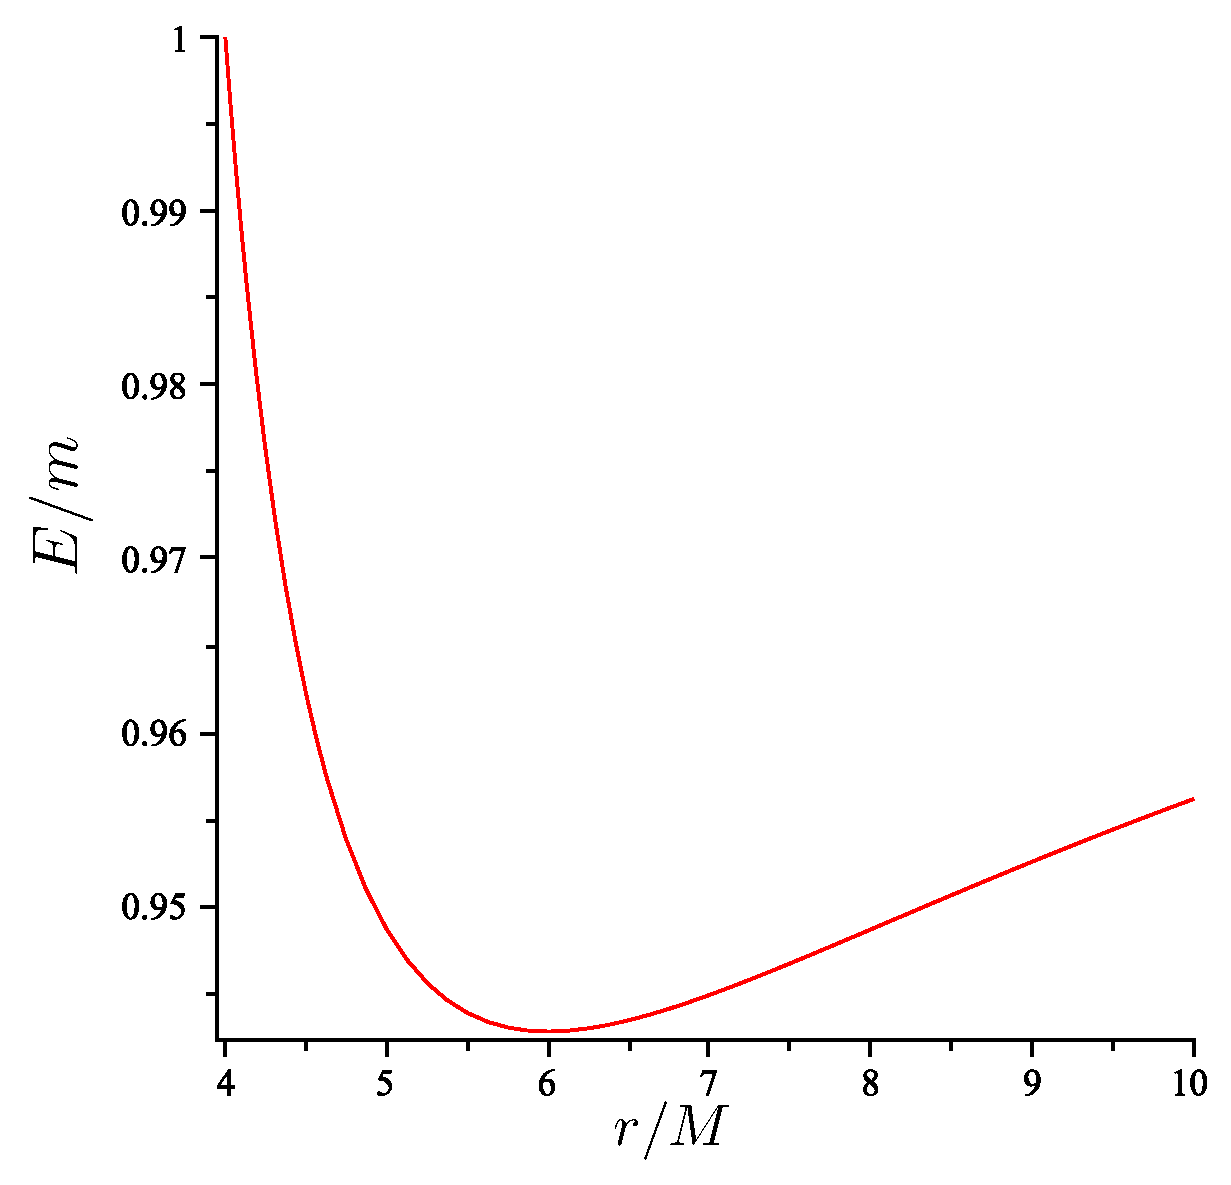
\includegraphics[width=4in]{figures/Eofrplot.pdf}
\caption{A plot of the energy-per-unit mass of a test particle orbiting a Schwarschild black hole as a function of its radial coordinate per the black hole's mass. The plot was created in Maple using equation \ref{eqn:Eschwarz}.}
\end{figure}

\subsection{The Post-Newtonian Expansion}




\Chapter{The LIGO Gravitational Wave Detectors}
\label{ch:ligo_detectors}
The fact that matter responds to gravitational waves as described in
Sec.~\ref{sec:effects_of_waves} offers the possibility of making a
direct detection of such waves.  Although several methods of detection
have been proposed, we focus here on that used by LIGO and, with some
minor differences, Virgo and GEO.  Again, this presentation will be of
necessity brief.  We refer readers to the textbook by
Saulson~\cite{Saulson:1994} for a much more comprehensive treatment.

Throughout this and the following chapters we will refer to 
the entire apparatus as an \emph{Interferometric Observatory}
(IFO), \emph{detector} and \emph{instrument} interchangeably.

\section{A Toy Model}

We motivate our discussion of the LIGO interferometers with a toy
model.  We wish to detect gravitational waves, and one method is
suggested by the analysis of the preceding chapter; we look for the
strain, $\Delta L/L$, by measuring change in length of some system.
Simply measuring a length with a ruler will not work, as any ruler
will itself be stretched and compressed by the wave.  However, we can
also measure distance by sending a projectile, say a marble, with
known velocity through the length and measuring the travel time.  To
avoid complex issues of synchronizing clocks at different points in
general relativity we add a (hypothetical perfectly elastic) rubber
wall at the far end, and measure how long it takes to return.  If the
velocity of the marble is much larger than the velocity of the wall
induced by the wave (that is, $v \gg h \omega L$ where $h$ is the
strain and $\omega$ the gravitational-wave frequency) then there is a
simple relationship between the round-trip travel time and the
amplitude of the wave.  However, this requires unrealistic precision
in measurement, the uncertainty in the marbles' launch time will swamp
the small changes in length since, as we will see in the next chapter,
$h$ is typically very small.

Therefore, we instead construct a \emph{null experiment} where we try
to determine if a given quantity is exactly zero.  We arrange two
perpendicular paths, fire marbles down each at the same time and
measure the difference in return times.  As gravitational waves are
rare, we ``lock'' the system by shifting one or both of the walls such
that the marbles always collide exactly (say by measuring their recoil
angle).  Once locked, deviations in the length of either or both arms
will cause the difference in arrive times to become non-zero, which
can be determined by a change in the marbles' recoil angles or lack of
collision entirely.

To obtain robust results we want $\delta L$ to be as large as
possible.  Since gravitational waves are week, this means increasing
$L$.  Practical concerns may limit the ability to do this.  For
example, clearly the entire path from source to walls must be in
vacuum in order for the marbles not to lose energy, and building large
vacuum systems is difficult and expensive.  We therefore use a trick
and add a second set of walls between the source and reflectors, and
arrange the paths so that the marbles bounce back and forth several
times before returning to the source.  This effectively extends $L$ by
the distance between the two surfaces multiplied by the number of
bounces.

Our final extension to this toy model is rather unrealistic, but
imagine that marbles vanish after a collision.  Our ability to detect a
gravitational wave with statistical confidence then reduces to our
ability to count marbles.  We can model this as a Poisson process, where
probability of observing $N$ marbles is 
%
\begin{equation*}
p(N) = \frac{\bar{N}^N \exp(-\bar{N})} {N!}
\end{equation*}
%
where $\bar{N}$ is the average expected number of marbles per
observation period.  The error in estimating $N$ from counting goes as
$1/\sqrt{N}$, and it is therefore advantageous to send out as many 
marbles as possible.

\section{Interferometric Gravitational Wave Detectors}

The toy model presented above captures the essential principles behind
LIGO, with the significant difference that light is used instead of
marbles.  A cartoon of the LIGO instruments is shown in
Fig.~\ref{f:ligo}.  The laser, beam splitter and two inner mirrors
(labeled \texttt{ITMX} and \texttt{ITMY} for ``inner test masses'')
form a \emph{Michelson interferometer}, and parallel the original toy
model with two marbles and two reflecting surfaces.

\begin{figure}
  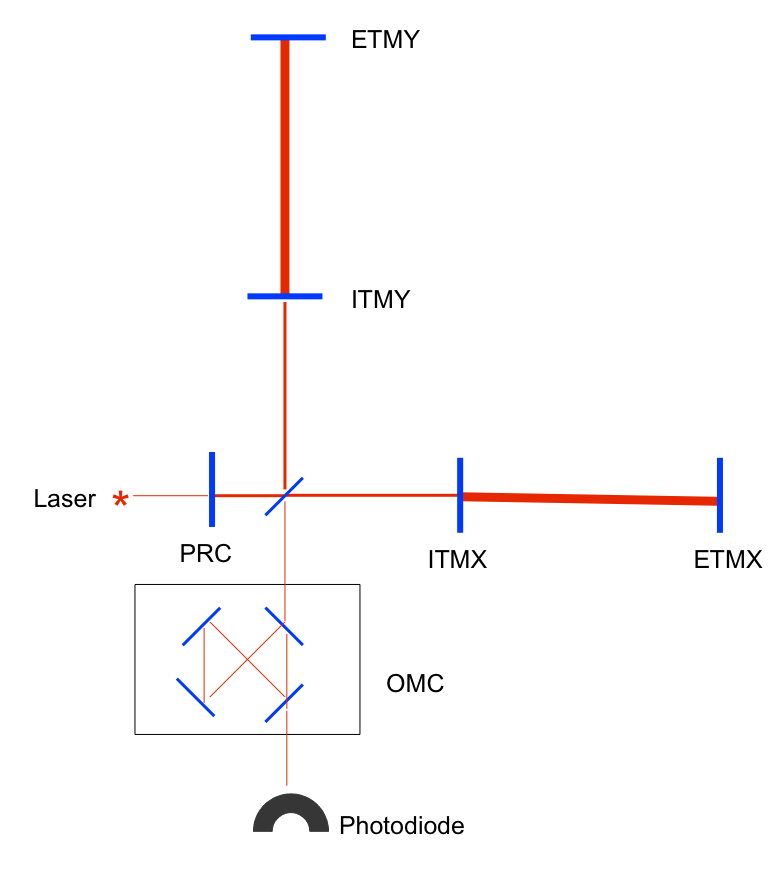
\includegraphics[width=\linewidth]{figures/detectors/LIGO}
  \caption[Block diagram of LIGO]{
  \label{f:ligo}
Block diagram of LIGO, see the text for description.
}
\end{figure}%
The use of light actually simplifies the analysis because light
travels on null geodesics, so
%
\begin{equation*}
ds^2 = 0 = g_{\mu\nu} dx^\mu dx^\nu
\end{equation*}

We now consider a +-polarized gravitational wave travelling in the $z$
direction, and place the arms on the $x$ and $y$ axes.  We again
assume the frequency of the wave is large compared to the travel time
between the arms, which implies that, over the round trip, $h_+$ may be
taken to be constant and the metric becomes
%
\begin{equation*}
g_{\mu\nu} = -dt^2 + (1+h_+) dx^2 + (1-h_+) dy^2 + dz^2
\end{equation*}
%
Then for the $x$ axis, restoring physical units,
%
\begin{equation*}
c^2 dt^2 = (1+h_+) dx^2
\end{equation*}
%
and the round-trip travel time is
%
\begin{equation*}
t_x = \frac{2L}{c} \sqrt{1+h_+} \approx \frac{2L}{c} \left(1+\frac{h_+}{2} \right)
\end{equation*}
%
where we approximate the square root by its Taylor series and ignore
higher-order terms in $h_+$.  Similarly the round-trip light travel
time along the $y$ arm is
%
\begin{equation*}
t_y = \frac{2L}{c} \left(1-\frac{h_+}{2} \right)
\end{equation*}

Considering a single wavefront leaving the beam splitter, the
difference in return time is
%
\begin{equation*}
\Delta t = t_x - t_y = \frac{2L}{c} h_+
\end{equation*}

In interferometry we measure the difference in phase between returning
wavefronts.  This difference will cause an interference pattern that
will serve as the readout.  If we use laser light of frequency $f$ and
wavelength $\lambda = c/f$ then a time difference of $\Delta t$
corresponds to a phase difference of 
%
\begin{equation*}
\Delta \Phi = \frac{2\pi f}{\Delta t} = \frac{4\pi f L}{c} h_+
= \frac{4\pi L}{\lambda} h_+
\end{equation*}

As in the marble example, we can increase the sensitivity of the
instrument by increasing $L$, but practical considerations prevent us
from doing so.  One of these considerations is in fact the same for
marbles and light; the travel path must be in vacuum.  We
therefore employ the same trick and add two additional mirrors,
indicated as \texttt{ETMX} and \texttt{ETMY} (for ``end test
masses'').  The addition of these mirrors creates a \emph{Fabry-Perot
cavity} in each arm.  By arranging the mirrors to be an integer
number of wavelengths apart a resonance is built up that can trap the
light for extended periods, approximately 200 bounces.  It can be seen
that if the mirrors are not appropriately spaced there will be
destructive interference between the light moving in different
directions.  As the power in the beam must be conserved, this results
in energy leaking out of the cavity, reducing the efficiency.

The addition of the Fabry-Perot cavities would suggest an increase in
phase difference of two orders of magnitude.  However, it is in fact
better than that.  The light is now in flight sufficiently long that,
for gravitational waves from astrophysical sources, $h_+$ will have
changed during the interval and the above analysis is no longer
valid.  A more careful analysis shows that the improvement is 
three orders of magnitude.

In interferometry it is typically most useful to think of light as a
wave.  However, where in the toy example our ability to detect
gravitational waves was limited by our ability to count marbles, in
real LIGO we are limited by our ability to count photons.  Photon
number is related to laser energy by $E=h\nu$, so we therefore want to
use as powerful a laser as possible.  There are, however, technical
obstacles to doing so.  In the latest LIGO run the laser power was up
to 14 W, although it was not always possible to run at this level.

In lieu of raising the laser power we can at least ensure that no
power is wasted.  LIGO is configured such that the beams interfere
destructively when they recombine, we say the instrument sits on a
\emph{dark fringe}~\footnote{Actually if we sat exactly on a dark
fringe then any change in the arm lengths would cause an increase of
light at the readout, and we would be unable to determine in which
direction the mirrors were moving.  We therefore sit a bit off the
dark fringe.}.  By conservation of energy all the power emitted by the
laser must go back towards the laser (neglecting the portion lost to
scattering, absorbed by the mirrors, etc).  We can recover this power
by adding another mirror, indicated on the diagram as \texttt{PRC}, or
power-recycling cavity.

The final feature on Fig.~\ref{f:ligo} is the \texttt{OMC} (output
mode cleaner), which was an important addition to the latest science
run.  A full description of this element is outside the scope of this
thesis, but we note briefly that the cross-section of a laser beam can
be decomposed into Hermite-Gaussian modes, as in
Fig.~\ref{f:hermite_gauss}.  The higher-order modes, being
non-symmetric, can induce angular instabilities in the mirrors.  It is
therefore advantageous to suppress such modes.

\begin{figure}
  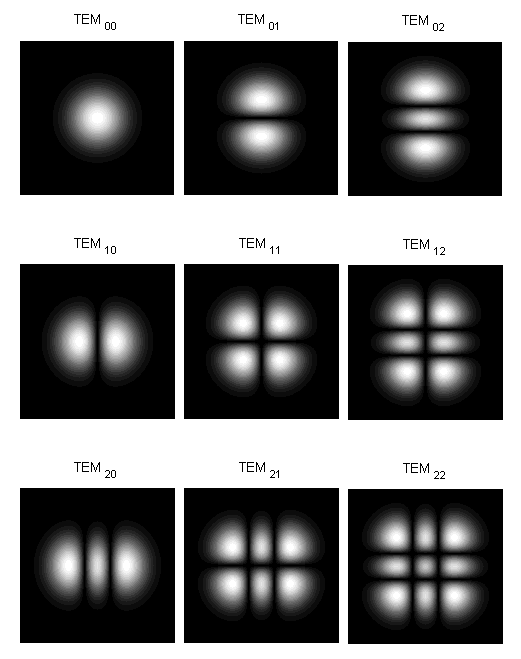
\includegraphics[width=\linewidth]{figures/detectors/TEMmn}
  \caption[Laser modes]{
  \label{f:hermite_gauss}
Basis functions for the cross-sectional distribution of power in a
laser beam.  The lack of symmetry in the higher-order modes can induce
instabilities in the LIGO optics. (\it{Public-domain image taken from
Wikipedia}~\cite{wikipedia:temmn})
}
\end{figure}%

\subsection{Readout}
\label{ssec:readout}

In order to operate correctly the two Fabry-Perot cavities and the
power-recycling mirror must be positioned such that the light is
resonant.  The Michelson must likewise by arranged so that the output
photodetector is on a dark fringe.  When the instrument is in this
state we say it is \emph{locked}, at that point a gravitational wave
will perturb the system within limits and produce light out the
output.  However, the resonances must be very finely tuned and left
untouched the system would quickly fall out of lock due to random
motions of the mirrors.  There is therefore a need for continuous,
active corrections implemented by a system of sensors and servos
throughout the instrument.

Ignoring the OMC there are five degrees of freedom in
Fig.~\ref{f:ligo}: the two initial test masses, the two end masses,
and the PRC.  Each of these is individually measured and controllable.
However, it is more convenient to consider various linear combinations
of these degrees of freedom:

\begin{itemize}
\item \texttt{DARM}: the differential motion of the two end test masses
\item \texttt{CARM}: the common motion of the two end test masses
\item \texttt{MICH}: the differential motion of the ``small Michelson'' comprising
the ITMs and the beam splitter
\end{itemize}

One of the sensors used to keep the system on resonance is the output
photodector.  Along with this, note that \texttt{DARM} is the quantity
of interest in the experiment, the change in length produced by a
gravitational wave.    It turns outs that rather than reporting the
signal at the photodiode directly a better output is the extent to
which this degree of freedom is off the resonance condition, which is
recorded as \texttt{DARM\_ERR}.  Henceforth, and especially in
chapter~\ref{ch:detchar} we consider this ``the output of the
detector''.  It is not, however, the data stream in which we will
search for gravitational waves.  The detector output needs to be
calibrated with respect to the instrument's frequency response.  This
can be measured by injecting a sine wave of known amplitude into the
system by actuating one of the mirrors, and measuring the amplitude
and phase of \darmerr.  The result is a complicated function of
frequency.  This can then be inverted to map \darmerr back to the true
input, the result is stored as \texttt{LSC-STRAIN} (for \emph{Length
Sensing and Control}, and it is that channel on which
gravitational-wave searches are performed.

\subsection{Noise Sources}
\label{sec:noise_sources}

In addition to gravitational-wave sources the instrument is subject to
various other influences collectively known as noise.  One class of
noise can be modeled as a \emph{Gaussian random process}, as we will
discuss in the next chapter.  These are best characterized by their
frequency profiles.  The dominant source are:
%
\begin{itemize} 
\item \emph{Seismic noise} is due to the coupling of the
instrument to the ground.  Much work has been been done, and much
research continues to be done, to isolate the mirrors from the
environment.  However, the isolation is not complete.  This noise
source dominates at low frequency, rising sharply below 40 Hz in
Initial LIGO.  In Advanced LIGO we hope to push this so-called
\emph{seismic wall} down to 10 Hz.  This noise source includes the
natural constant vibrations of the Earth, wind blowing over nearby
structures, and anthropogenic sources such as vehicles near the sites,
logging activity, etc.

\item \emph{Thermal noise}. Any system possesses energy proportional
to the product of Boltzmann's constant and the ambient temperature.
This energy manifests as random motion throughout the detector,
although the motion from the test masses and the wires from which they
are hung are the largest contributors to noise.  The noise produced
dominates from 40 Hz to approximately 200 Hz.

\item \emph{Shot noise} is the uncertainty inherent in counting
photons, as discussed above.  It increases with frequency and
dominates above $\approx 1$ kHz.

\end{itemize}
%
In addition to these broad-band sources of noise there are also
\emph{lines}, particular frequencies at which the noise is much
greater than the three sources above would produce.  Two of the most
significant are:
%
\begin{itemize}
\item \emph{Electrical noise}.  Despite shielding, at 60 Hz there is a
sharp increase in the noise level due to the frequency of the US
electrical grid.
\item \emph{Violin modes}.  Although the wires suspending the mirrors
vibrate over a range of frequencies due to thermal noise, the
suspension system has a resonance at about $340 Hz$, producing much
more noise here.
\end{itemize}
%
There are also lines at higher harmonics of these frequencies.

In addition to these continuous noise sources there are numerous
\emph{glitches}, short transient events.  These glitches have a wide
variety of different morphologies and originate from many different
sources.  Some glitches are reactions to external environmental
conditions and others are internal to the detector.  As one
straightforward example, a heavy object dropped on a nearby road 
can, through seismic coupling, shake the mirrors and produce a sharp
``bang'' in \darmerr.

At the most abstract level gravitational-wave searches entail looking
for features in the data that deviate in some way from the continuous
background.  It is therefore not surprising that glitches can
interfere with searches and hence must be removed to the extent
possible.  Chapter~\ref{ch:segdb} will present the infrastructure used
to store information about the state of the detector and environment,
and chapter~\ref{ch:detchar} will discuss part of the effort to
identify glitches and remove them from the analysis.

\section{Conclusions}

In this chapter we reviewed the basic elements of interferometric
gravitational-wave detectors.  In the next chapter we discuss how we
search the data obtained by these detectors for signals of the kind
described in the previous chapter.



\Chapter{Searching for Gravitational Waves from Compact-Binary
Coalescences}
\label{ch:search}

% from Boyle et al.
\subsection{Matched filtering}
\label{sec:MatchedFiltering}

Current searches for gravitational waves from binary black-hole
coalescence use matched filtering to search for a waveform buried in
noise.  The matched filter is the optimal filter for detecting a
signal in stationary Gaussian noise.  Suppose that $n(t)$ is a
stationary Gaussian noise process with one-sided power spectral
density $S_n(f)$ given by $\langle \tilde{n}(f) \tilde{n}^\ast(f')
\rangle=\frac{1}{2} S_n(|f|)\delta(f-f')$.  For long integration
times, the data stream $s(t)$ output by the detector will always be
dominated by the noise.  Thus, we can simply approximate $n \approx s$
to calculate $S_{n}(f)$.

Using this power spectral density (PSD), we can define the inner
product between two real-valued signals---the data stream $s$ and the
filter template $h$---by
\begin{eqnarray}
  \label{eq:InnerProduct}
  \InnerProduct{s|h} &\equiv 2\, \Re \int_{-\infty}^{\infty}\,
  \frac{\tilde{s}(f)\, \tilde{h}^{\ast}(f)}{S_{n}(\lvert f
    \rvert)}\, d f \\ &= 4\, \Re \int_{0}^{\infty}\,
  \frac{\tilde{s}(f)\, \tilde{h}^{\ast}(f)}{S_{n}(f)}\, d f\ .
\end{eqnarray}
Then, given data $s$ which may contain either noise $n$ or noise and a
gravitational wave signal $h$,
\begin{equation}
  s = \left\{\begin{array}{l}
      n  \\
      n+h
    \end{array} \right.\ ,
\end{equation}
the matched-filter signal-to-noise ratio (SNR) is defined as
\begin{equation}
  \label{eq:InnerProductSNR}
  \rho = \frac{1}{\sqrt{\InnerProduct{h|h}}} \InnerProduct{s|h}\ .
\end{equation}


The SNR can then be used to construct a detection statistic (directly
or in combination with other statistics).  It is therefore important
to ensure that the templates used in searches accurately model the
expected waveforms to avoid reduction in the value of $\rho$. The
\emph{overlap} between two templates $h$ and $h'$ is defined as
\begin{equation}
  \label{eq:OverlapDefinition}
  \Overlap{h|h'} \equiv \frac{\InnerProduct{h|h'}}{
    \sqrt{\InnerProduct{h|h} \InnerProduct{h'|h'}}}\ .
\end{equation}
The overlap encodes the fractional loss in SNR that results from using
the template $h'$ rather than the true waveform $h$.  In a search that
uses $\rho$ as a detection statistic this corresponds to the
fractional loss in distance to which the search is sensitive.

The filter template includes arbitrary time and phase offsets, encoded
by the arrival time and phase, $\ta$ and $\phia$.  Under a change of
these quantities, the Fourier transform behaves as
\begin{equation}
  \label{eq:EffectOfTimeAndPhaseOffset}
  \tilde{h}(f) \to \tilde{h}(f)\, \e^{-2\pi i f \ta - i \phia}\ .
\end{equation}
We maximize over these two variables by calculating the inner product
as

\begin{eqnarray}
  \max_{\ta, \phia}\, \InnerProduct{s|h}
  &= \max_{\ta, \phia}\, 4\, \Re \int_{0}^{\infty}\,
  \frac{\tilde{s}(f)\, \tilde{h}^{\ast}(f)}{S_{n}(f)}\, \e^{2\pi i
    f\ta + i \phia}\, d f
  \\
  & = 4 \max_{\ta}\, \left\lvert \int_{0}^{\infty}\,
    \frac{\tilde{s}(f)\, \tilde{h}^{\ast}(f)}{S_{n}(f)}\, \e^{2\pi i
      f\ta}\, d f \right\rvert\ .
\end{eqnarray}
Note that this integral is just the (inverse) Fourier transform of the
quantity $\tilde{s}(f)\, \tilde{h}^{\ast}(f) / S_{n}(f)$ evaluated at
$\ta$.  Thus finding the maximum over $\ta$ involves taking the
Fourier transform and selecting the largest element of the finite set
that results from discretization.


\Chapter{Comparison of Numerical Simulations of
Black-Hole Binaries with Post-Newtonian Waveforms}
\label{ch:comparison}
\newcommand{\Note}[1]{\textcolor{red}{\textbf{[#1]}}}
\newcommand{\Add}[1]{\textcolor{blue}{#1}}
%\renewcommand{\d}{\mathrm{d}}
%\renewcommand{\e}{\mathrm{e}}
%\renewcommand{\i}{\mathrm{i}}
\newcommand{\hyb}{\mathrm{hyb}}
\newcommand{\NR}{\mathrm{NR}}
\newcommand{\pN}{\mathrm{pN}}
\newcommand{\ADMMass}{M_{\mathrm{ADM}}}
\newcommand{\IrrMass}{M_{\mathrm{AH}}}
\newcommand{\MSun}{\ensuremath{M_{\odot}}}
\newcommand{\deff}{\ensuremath{D_{\mathrm{eff}}}} % effective distance
\newcommand{\ta}{\ensuremath{t_{\mathrm{a}}}}
\newcommand{\phia}{\ensuremath{\phi_{\mathrm{a}}}}
\newcommand{\fsamp}{\ensuremath{f_{\mathrm{s}}}}
\newcommand{\fNy}{\ensuremath{f_{\mathrm{Ny}}}}
\newcommand{\discretize}{\rightsquigarrow}
\newcommand{\software}[1]{\textsc{#1}}
\newcommand{\etal}{\textit{et al.}\xspace}
\newcommand{\G}{G}
\renewcommand{\c}{c}
\newcommand{\e}{e}
%\newcommand{\lvert}{\ensuremath{|}}
%\newcommand{\rvert}{\ensuremath{|}}

%%% Define \InnerProduct with extendible middle line
%%% Adapted from braket.sty
\makeatletter
\let\protect\relax
{\catcode`\|=\active
  \xdef\InnerProduct{\protect\expandafter\noexpand\csname InnerProduct \endcsname}
  \expandafter\gdef\csname InnerProduct \endcsname#1{%
    \begingroup
    \ifx\SavedDoubleVert\relax
    \let\SavedDoubleVert\|\let\|\IpDoubleVert
    \fi
    \mathcode`\|32768\let|\IPVert
    \left({#1}\right)
    \endgroup
  }
}
\def\IPVert{\@ifnextchar|{\|\@gobble}% turn || into \|
     {\egroup\,\mid@vertical\,\bgroup}}
\def\IPDoubleVert{\egroup\,\mid@dblvertical\,\bgroup}
\let\SavedDoubleVert\relax
\def\midvert{\egroup\mid\bgroup}
\def\SetVert{\@ifnextchar|{\|\@gobble}% turn || into \|
    {\egroup\;\mid@vertical\;\bgroup}}
\def\SetDoubleVert{\egroup\;\mid@dblvertical\;\bgroup}
\def\mid@vertical{\mskip1mu\vrule\mskip1mu}
\def\mid@dblvertical{\mskip1mu\vrule\mskip2.5mu\vrule\mskip1mu}
\makeatother


\Note{Numbers in this chapter are subject to change after 
completing the reruns to fix the sign error in the 
3pN term}

\section{Introduction}
\label{sec:Introduction} %

In chapter~\ref{ch:search} we outlined the CBC pipeline used to search
LIGO/Virgo data for gravitational waves resulting from the inspiral of
binary systems composed of neutron stars and/or black holes.  In
particular we noted the use of post-Newtonian templates of the form
discussed in section~\ref{sec:PNWaveforms} to filter the data up to a
total mass of $25 \msun$.  The post-Newtonian approximation is valid
so long as the velocities of the component masses are small compared
to the speed of light, or equivalently so long as the orbital
frequencies are small.  Frequently the waveform is terminated at the
Schwarzschild ISCO frequency, after which the inspiral transitions to
a plunge, although this is only strictly correct in the point-mass
limit.

For systems containing two neutron stars this frequency is above 1000
Hz, even for a hypothetical system composed of two instances of the
heaviest-known neutron star.  This is well outside LIGO's most
sensitive band where most of the SNR will be accumulated, and we may
therefore trust pN waveforms for a BNS search.  However, for systems
including at least one black hole the ISCO frequency will be lower and
the merger may occur in the sensitive band.  It is therefore
important to test the ability of pN templates to detect such systems
and where possible optimize their use.  In order to evaluate the
effectiveness of templates it is necessary to compare the waveforms
against complete waveforms including the inspiral, merger and ringdown
phases.  This necessitates the use of hybrid pN-NR waveforms as
described in section~\ref{sec:HybridWaveforms}.  This chapter uses
high-accuracy waveforms developed at Caltech and Cornell~\footnote{The
code used to produce these waveforms, SpEC, is now being developed and
used by a collaboration including scientists at Caltech, Cornell and
the Canadian Institute for Theoretical Astrophysics (CITA).}. 

The most robust test would consider the ability of the full pipeline
to detect BBH signals; this is the goal of the NINJA project
introduced in the following chapter.  Here we focus on a more
fundamental question, the ability of pN waveforms to capture full
physical signals.  We test this by calculating the overlap (defined in
eqn.~\ref{eq:OverlapDefinition}) between the hybrid waveform and the
pN approximation.  If no instance of a waveform in the chosen pN model
provides a high overlap with the hybrid signal then the pipeline as a
whole will be unable to detect such signals.  A similar study has been
performed by Pan~\etal using numerical data from Pretorius and the
Goddard groups~\cite{Pan2007}.  Our main results are in agreement with
their conclusion that a simple extension of the TaylorF2 waveforms
currently in use by the CBC low-mass search yields high overlaps with
numerical waveforms.

Throughout this chapter we use only the $(l,m)=(2,2)$ component of the
waveform $\Psi_{4}^{2,2}$ (as defined, e.g., in~\cite{Boyle2008a}).
For convenience, we drop the superscript.  Whenever possible, we use
dimensionless quantities, like $r\,M\,\lvert \Psi_{4} \rvert$, where
$r$ is the areal radius of the observation sphere, and $M$ is the
total apparent-horizon mass of the holes in the initial data.
However, for any calculation involving the LIGO noise curve, we have a
physical scale, and thus use standard mks units.  

To weight the inner products in the overlap we use the
following PSDs for Initial and Advanced LIGO: for Initial LIGO we use
an analytic approximation to the LIGO design PSD given by
\begin{eqnarray}
  S_n(f) &= &3.136 \times 10^{-4} \bigg[
  \left(\frac{ 4.49 f}{150.0}\right)^{-56.0} \nonumber \\
  &+ & 0.16 \left(\frac{f}{150}\right)^{-4.52}
  + \left(\frac{f}{150.0}\right)^2 + 0.52
  \bigg]
\end{eqnarray}
All integrals start from 40 Hz.  As shown in
Fig.~\ref{fig:StildesAndInitialPSD}, at this frequency the noise is an
order of magnitude higher than its lowest value, and below this
frequency it rises rapidly as $\sim f^{-56}$.  The region below 40 Hz
therefore contributes very little signal power to the
SNR~\cite{Abbott:2007xi}.  

For Advanced LIGO we use the GWINC program~\cite{AdvancedLIGONoise} to
generate the PSD.  GWINC reports the PSD in increments of 0.0124 Hz.
When calculating discrete integrals against signals sampled at other
frequencies we obtain values for the PSD by linearly interpolating
between the values provided by GWINC.  We start integrals at 10 Hz as
that is the point where the noise has increased by two orders of
magnitude above its minimum, as also shown in
Fig.~\ref{fig:StildesAndInitialPSD}.




%%%%%%%%%%%%%%%%%%%%%%%%%%%%%%%%%%%%%%%%%%%%%%%%%%%%%%%%%%%%%%%%%%%%%%
%%%%%%%%%%%%%%%%%%%%%%%%%%%%%%%%%%%%%%%%%%%%%%%%%%%%%%%%%%%%%%%%%%%%%%
\section{PN--NR hybrid waveform}
\label{sec:PNNRHybridWaveform} %


In order to perform our comparison we need to construct a ``true''
black-hole binary waveform, which we might expect to observe with
detectors.  A numerical simulation provides the data for the crucial
nonlinear merger phase.  We carefully extract the data and extrapolate
it to large radius, and investigate the effects of numerical error on
the final result.  Because this waveform is very computationally
expensive to produce, it covers only about 32 cycles, which is not
sufficient for a thorough investigation of the possibility of
detecting it in searches of data from gravitational-wave detectors.
Thus, we match the numerical waveform to a post-Newtonian waveform,
producing a hybrid which extends for many thousands of cycles,
covering the entire band of interest.

\subsection{Numerical simulation, extraction, and extrapolation}
\label{sec:WaveformExtractionAndExtrapolation}
The numerical simulation is the same as that described in
Refs.~\cite{Boyle2007, Scheel2008}: an equal-mass, non-spinning,
black-hole binary with reduced
eccentricity~\cite{Pfeiffer-Brown-etal:2007}, beginning roughly 16
orbits before merger, continuing through merger and
ringdown~\cite{Scheel2008}.  It is performed with the Caltech--Cornell
pseudospectral code, using boundary conditions designed to prevent
constraint violations and gravitational radiation from entering the
domain~\cite{Holst2004, Lindblom2006}.

Data is extracted from the simulation in the form of the
Newman--Penrose scalar
\begin{equation}
  \Psi_{4} = -C_{\alpha \beta \gamma \delta} l^{\alpha}
  \bar{m}^{\beta} l^{\gamma} \bar{m}^{\delta}\ ,
\end{equation}
where $l^{\alpha}$ and the complex vector $\bar{m}^{\beta}$ are
constructed with reference to the coordinate basis.  Along the
positive $z$ axis, we have
\begin{eqnarray}
  l^{\alpha} &= & \frac{1}{\sqrt{2}}\, \left( t^{\alpha} - z^{\alpha}
  \right)\ , \\
  \bar{m}^{\beta} &= & \frac{1}{\sqrt{2}}\, \left(
    \frac{\partial}{\partial x} - i\, \frac{\partial}{\partial y}
  \right)^{\beta}\ .
\end{eqnarray}

Here, $t^{\alpha}$ is the timelike unit normal to the spatial
hypersurface, and $z^{\alpha}$ is the unit vector in the positive $z$
direction.  The vectors $\partial/\partial x$ and $\partial/\partial
y$ are the standard coordinate vectors, which are not normalized.
$\Psi_{4}$ is extracted as a function of time, at various radii along
the positive $z$ axis.  This is then extrapolated to large radii, as
described in Ref.~\cite{Boyle2007}, and in greater detail in
Ref.~\cite{Boyle2008}.

% The Nyquist frequency of the data is \Note{bla, as compared to the
%   measured ringdown frequency}.  Note that the LIGO Nyquist
% frequency is \unit[2048]{Hz}, which is lower than the ringdown
% frequency for masses above bla.

The measured (instantaneous) frequency at the beginning of the
simulation is
\begin{equation}
  \label{eq:MeasuredStartingFreq}
  % \frac{G\,M}{c^{3}}\,\omega & = 0.0333 \pm 0.0002\ , \\
  % \frac{G\,M}{c^{3}}\,f & = 0.00530 \pm 0.00003\ , \\
  f_{\mathrm{initial}} = \unit[(1.08 \pm 0.01) \times 10^{3}]{Hz}\,
  \frac{\MSun}{M}\ .
\end{equation}
The measured ringdown frequency is
\begin{equation}
  \label{eq:MeasuredRingdownFreq}
  % \frac{G\,M}{c^{3}}\,\omega & = 0.553 \pm 0.007\ , \\
  % \frac{G\,M}{c^{3}}\,f & = 0.088 \pm 0.001\ , \\
  % \omega & = \unit[(112 \pm 1) \times 10^{4}]{\frac{1}{sec}}\,
  % \frac{\MSun}{M}\ , \\
  f_{\mathrm{ringdown}} = \unit[(1.78 \pm 0.02) \times 10^{4}]{Hz}\,
  \frac{\MSun}{M}\ .
\end{equation}
The measured \emph{Christodoulou} mass and spin of the final black
hole are
\begin{eqnarray}
  \label{eq:MeasuredFinalMass}
  M_{\chi\mathrm{, final}} &= &(0.95162 \pm 0.00002)\, M_{\chi\mathrm{,
      initial}}\ , \\
  \label{eq:MeasuredFinalSpin}
  S_{\mathrm{final}} &= &(0.68646 \pm 0.00004)\, M^{2}_{\chi\mathrm{, final}}\ .
\end{eqnarray}
Using this value for the spin, a quasi-analytic formula due to
Echeverria~\cite{Echeverria1989} predicts a value of
$\unit[1.77\times10^{4}]{Hz}\, \frac{\MSun}{M}$, for the ringdown
frequency, in close agreement with the measured frequency.

\subsection{Accuracy of the numerical simulation}
\label{sec:Accuracy}

The numerical waveform will be the standard against which we will
judge the \textit{TaylorF2} waveforms used in LIGO data analysis.  To
understand how precisely we should trust our final results, we need to
understand the accuracy of the waveform itself.  The most obvious
measure of the error in this fiducial waveform is its convergence with
increasing numerical resolution.  Fig.~\ref{f:accuracy} shows the
overlap (Eq.~\eqref{eq:OverlapDefinition}) between waveforms computed
at different resolutions.  The data used here are the extrapolated
$\Psi_4$ waveforms, integrated in time twice.
%%%%%%%%%%%%%%%%%%%%%%%%%%%%%%%%%%%%%%%%%%%%%%%%%%%%%%%%%%%%%%%%%%%%%%
\begin{figure}
  \begin{center}
    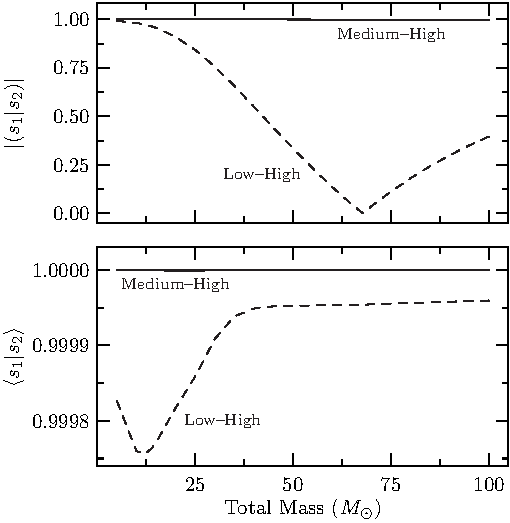
\includegraphics[width=0.55\linewidth]{figures/comparison/Accuracy}
  \end{center}
  \caption[Convergence testing for numerical waveforms ]{
  \label{f:accuracy}
    Convergence testing for numerical waveforms from a
    data-analysis perspective, using the match between waveforms
    computed at different numerical resolutions.  The waveforms are
    scaled to various masses, and the Initial-LIGO noise curve is used
    in the calculation of the match.  The upper panel shows the
    overlap without maximization over arrival time and phase; the
    lower panel shows the overlap after maximization.  In each panel,
    the lower (dashed) line compares the lowest- and
    highest-resolution simulations, while the upper (solid) line
    compares the medium- and highest-resolution simulations.  Note
    that this plot uses only numerical data, with no post-Newtonian
    contribution.}
\end{figure}%
%%%%%%%%%%%%%%%%%%%%%%%%%%%%%%%%%%%%%%%%%%%%%%%%%%%%%%%%%%%%%%%%%%%%%%

Because of the short extent of the numerical waveforms, we need to be
careful when using their Fourier transforms.  The signal can be
corrupted easily by the non-periodicity of the waveforms, and the
discontinuous jumps that result.  For Fig.~\ref{f:accuracy} we
mitigate this problem by increasing the sampling frequency of the
input data, and restricting the Fourier transform to frequencies
corresponding to instantaneous frequencies contained in the data.  The
input data can easily be upsampled in the time domain by interpolating
the phase and amplitude of the complex data to a finer time grid.  We
then perform the transform, and explicitly set the data to zero at
frequencies below $f_{\mathrm{initial}}$ and above
$f_{\mathrm{ringdown}}$, as given in
Eqs.~\ref{eq:MeasuredStartingFreq} and~\ref{eq:MeasuredRingdownFreq}.
While the results do depend on whether or not we impose these cutoffs,
they do not depend sensitively on the actual cutoff frequencies.

The overlap between the lowest- and highest-resolution simulations
(dashed lines) actually passes through zero, as shown in the upper
panel.  Presumably, this is because of loss of phase accuracy over the
course of the simulation.  All three simulations begin with the same
initial data, so the waveforms are most similar at the beginning.
Masses for which this is the most important segment (the lowest
masses) will naturally have the highest overlap between resolutions.
As the simulation progresses, numerical error accumulates---notably in
the phase---so the overlap decreases with masses for which later
segments dominate the overlap (higher masses).  When the overlap is
optimized over arrival time and phase (sec.~/ref{sec:overlap}) we can
see that the overlap becomes much better, as shown in the lower panel,
indicating sufficient accuracy within any frequency band for which
phase coherence is required.  In either case, the medium and highest
resolutions are much more nearly the same.  Without optimization,
their overlap is within a few tenths of a percent of 1; after
optimization, the overlap is within $10^{-6}$ of 1.

In the rest of our analysis we use the highest-resolution waveform.
Because we always optimize over arrival time and phase, the lower
panel of Fig.~\ref{f:accuracy} is the most relevant, and shows that
the waveform has converged to very high accuracy.  The overlaps we
quote below will only be given to three decimal places at most,
because this is roughly the accuracy of the single-precision numerical
methods used in the rest of the chapter.  This accuracy is also
sufficient for searches of gravitational-wave data.  Thus, the
truncation error of the simulated waveform is irrelevant for those
purposes.

Other sources of error include residual eccentricity and spin, the
influence of the outer boundary of the simulation, extrapolation
errors, and coordinate effects, as discussed in Ref.~\cite{Boyle2007}.
The eccentricity had a disproportionately large effect on the error
quoted in that paper because of the matching technique, which is not
used here.  Restricting attention to the other effects of
eccentricity, the uncertainty falls below that due to numerical error.
Similarly, using the techniques of Ref.~\cite{Lovelace2008}, the
initial spins of the black holes have been measured more reliably, and
found to be more than an order of magnitude smaller than previously
determined, allowing us to reduce the estimate for that error to less
than the numerical truncation error.  The various coordinate effects
were all estimated to be of roughly the same magnitude as the
numerical error.

With the numerical error being many times more accurate than needed
for this analysis, and the other sources of uncertainty being of
roughly the same size, these considerations indicate that the overall
error in our fiducial waveform is substantially less than the
precision needed for this analysis.


%%%%%%%%%%%%%%%%%%%%%%%%%%%%%%%%%%%%%%%%%%%%%%%%%%%%%%%%%%%%%%%%%%%%%%
%%%%%%%%%%%%%%%%%%%%%%%%%%%%%%%%%%%%%%%%%%%%%%%%%%%%%%%%%%%%%%%%%%%%%%
\section{Detection efficiency of gravitational-wave templates}
\label{sec:Efficiency} %

We now compare the signal described in the previous section to
restricted, stationary phase \textit{TaylorF2} post-Newtonian
templates with terms up to order 2.0, order 3.5, and a ``pseudo-4.0
pN-order'' term recommended in Ref.~\cite{Pan2007}.  Overlaps are
calculated using the techniques of Sec.~\ref{sec:ihope_match_filter}
with the signal $s$ being the hybrid waveform described in the
previous section, scaled to a range of masses.  We consider both the
Initial- and Advanced-LIGO noise curves.

Plots of the hybrid waveforms in comparison to the Initial-LIGO noise
curve are shown in Fig.~\ref{fig:StildesAndInitialPSD}.
%%%%%%%%%%%%%%%%%%%%%%%%%%%%%%%%%%%%%%%%%%%%%%%%%%%%%%%%%%%%%%%%%%%%%%
\begin{figure}
  \begin{center}
    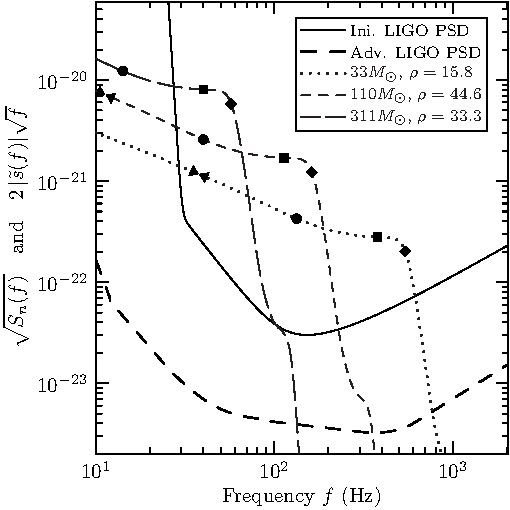
\includegraphics[width=0.55\linewidth]{figures/comparison/StildesAndInitialPSD}
  \end{center}
  \caption[Hybrid Caltech--Cornell waveform scaled to various total masses]{
  \label{fig:StildesAndInitialPSD}
    Hybrid Caltech--Cornell waveform scaled to various total
    masses, with sources optimally oriented and placed at
    \unit[100]{Mpc}, shown against the Initial- and Advanced-LIGO
    noise curves.  Markers are placed along the lines at frequencies
    corresponding to various instantaneous frequencies of the
    waveforms.  The triangles represent the beginning and end of the
    blending region; the circle represents the ISCO frequency; the
    square the light-ring; and the diamond the measured ringdown
    frequency.  See the text for discussion of the normalization.  The
    values given for $\rho$ use the Initial-LIGO noise curve, with
    sources at a distance of 100\,Mpc.}
\end{figure}%
%%%%%%%%%%%%%%%%%%%%%%%%%%%%%%%%%%%%%%%%%%%%%%%%%%%%%%%%%%%%%%%%%%%%%%
The masses are chosen so that various frequencies of interest (the
final stitching frequency, the ISCO, and the ringdown) occur at the
``seismic wall'' for Initial LIGO: \unit[40]{Hz}.  The waveforms
$\tilde{s}$ are scaled to depict the detectability of the signal,
typically quantified by the SNR introduced in
~\eqref{eq:InnerProductSNR}, which may be written as
\begin{equation}
  \label{eq:SNR}
  \rho^{2} \equiv \int_0^\infty \frac{4\, \tilde{s}(f)\,
    \tilde{s}^\ast(f)} {S_n(f)}\, d f = \int_0^\infty
  \frac{\left\lvert 2\, \tilde{s}(f)\, \sqrt{f} \right\rvert^{2}}
  {S_n(f)}\, d\ln{f}\ .
\end{equation}
In the final expression, the numerator and denominator have the same
units, and are directly comparable.  Because the square root of the
denominator is familiar, we plot that along with the square root of
the numerator.  Plotting these two quantities together gives a
graphical impression of the detectability of the waveform, and the
relative importance of each part of the waveform, by its height above
the noise curve.  In Ref.~\cite{BradyCreighton2002}, Brady and
Creighton define a slightly different quantity, the characteristic
strain $h_{\mathrm{char}} \equiv f\, \lvert \tilde{s}(f) \rvert\ .$
The relative factor of $\sqrt{f}$ they use is present so that they can
plot $h_{\mathrm{char}}$ against $\sqrt{f\, S_{n}(f)}$.  Cutler and
Thorne~\cite{Cutler2002} define still another quantity, the signal
strength $\tilde{h}_{s}(f)$, which is related to the Fourier transform
by $\tilde{h}(f) = \sqrt{5}\, \frac{T}{N}\, \tilde{h}(s)\ .$ The
factor of $\sqrt{5}$ comes from averaging over the orientation of the
binary, which we do not do.  $T/N$ is the ratio of the threshold to
the rms noise at the endpoint of signal processing.

\iffalse
\begin{figure}
  % \includegraphics[width=\linewidth]{figures/comparison/AmoebaHistogram}
  \begin{center}
    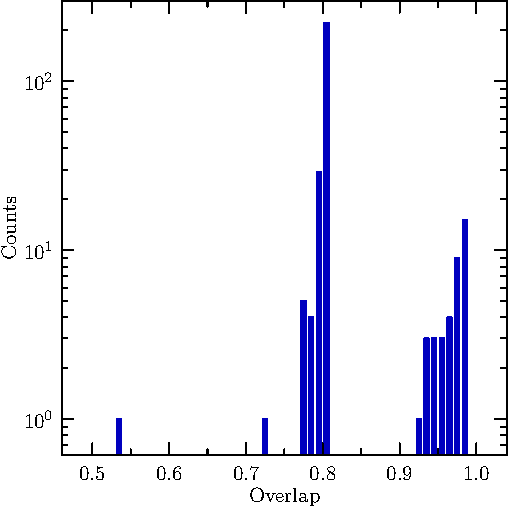
\includegraphics[width=0.55\linewidth]{figures/comparison/Histogram}
  \end{center}
  \caption{Histogram of overlaps found by 300 instances of the Amoeba
    algorithm, optimizing the overlap against a given waveform over
    $M, \eta, f_c$, with randomized initial conditions.  Note the
    logarithmic scale on the vertical axis.  The majority of instances
    produced a lower overlap than the optimum.  We interpret this as
    pointing to the existence of a broad local maximum which did not
    coincide with the global maximum.}
  \label{fig:AmoebaHistogram}
\end{figure}%
\fi

For each template family we initially optimize over signal mass $M$,
symmetric mass ratio $\eta = m_1 m_2 / (m_1 + m_2)^2$, and upper
cutoff frequency $f_c$.  The optimization is performed using a
Nelder--Mead (``amoeba'') algorithm~\cite{numrec_cpp}.  The amoeba
starts with a simplex in the parameter space and proceeds through a
series of steps, each of which will improve the value of the function
at at least one vertex.  The algorithm terminates when all vertices
have converged to the same point to within a specified tolerance.
This process is deterministic, and amounts to an enhanced
steepest-ascent algorithm.  It is therefore only guaranteed to find a
local maximum, and indeed we find that an amoeba instance started at a
random point in the parameter space is most likely to converge to a
point that does not give the highest possible overlap.  We interpret
this as being due to a large region in parameter space containing a
local maximum and a relatively smaller region containing the global
maximum.  We therefore supplement the basic amoeba by running 300
instances with random starting values, and taking the best match
obtained over all instances.  In repeated runs the same optimal
parameters were found by at least some of the amoebas, which supports
the claim that this is the true maximum.

The results of optimizing over all of $M, \eta$ and $f_c$ for selected
masses for Initial LIGO are given in
Table~\ref{tab:ThreeParamOverlapDetailInitial} and summarized in
Fig.~\ref{fig:ThreeParamOverlapSummaries}.  For Initial LIGO, in the
range covered by the current CBC low-mass search $(M < 35
\MSun)$~\cite{Abbott:2008}, the pseudo-4.0 pN \textit{TaylorF2}
waveforms achieve the highest overlaps, exceeding those obtained with
3.5 pN waveforms by $\sim 1\%$.  Above $35 \MSun$ the 3.5 pN waveforms
produce overlaps as much as 4\% greater than those obtained with
pseudo-4.0 pN waveforms over a range from $40$--$80 \MSun$. With the
Advanced-LIGO noise curve, in the CBC low-mass range, the 3.5 pN and
pseudo-4.0 pN waveforms produce overlaps within 2\% of each other,
with 3.5 pN producing higher overlaps below 20 $\MSun$ and pseudo-4.0
pN producing higher overlaps in the range $20$--$35 \MSun$.
Pseudo-4.0 pN continues to give the highest overlaps up to $60 \MSun$,
producing overlaps as much as 4\% greater than those obtained with 3.5
pN waveforms.  Above $60 \MSun$ 3.5 pN waveforms again yield the best
overlaps, by as much as 6\% around 90 $\MSun$.

% We see from Tables~\ref{tab:ThreeParamOverlapDetailInitial}
% and~\ref{tab:ThreeParamOverlapDetail} that the parameters of the
% optimal templates are often far from the parameters of the physical
% waveform, especially for high-mass systems, which emphasize portions
% of the waveform for which the pN and SPA assumptions are poor.  For
% Initial LIGO, pseudo-4.0 pN templates find $M$ to within $19\%$ of
% the true value compared to $52\%$ for 2.0 pN and $159\%$ for 3.5 pN.
% Conversely, for Advanced LIGO, 3.5 pN templates estimate the signal
% mass to within $16\%$ for masses less than $\MSun$, compared to
% $25\%$ for 2.0 pN and $20\%$ for pseudo-4.0 pN templates.

% \Note{Should we drop this paragraph?  We never systematically looked
%   at parameter estimation, and the numbers from the table don't tell
%   a compelling story regarding any of them doing better than the
%   others.}



% \addtolength{\tabcolsep}{3.25mm} \renewcommand{\arraystretch}{1.6}
\begin{table*}
  \begin{center}
    \begin{tabular}{@{}lcccc@{}}
      \hline \hline
      & $(10+10) \MSun$ & $(20+20) \MSun$ & $(30+30) \MSun$ & 
      $(50+50) \MSun$ \\
      \hline
      $\Overlap{s^{\textrm{NR-CC}} |
        h^{\textrm{SPA}_c^{\textrm{ext}}(2.0)}}$ &
      0.99 & 0.98 & 0.97 & 0.96 \\
      $M/\MSun$ &
      $23.27^{+0.13}_{-0.12}$  &
      $25.99^{+0.61}_{-0.56}$  &
      $35.22^{+1.84}_{-1.89}$  &
      $47.52^{+6.87}_{-4.73}$  \\
      $\eta$ &
      $0.199^{+0.0030}_{-0.0030}$  &
      $0.771^{+0.0490}_{-0.0420}$  &
      $1.000_{-0.1390}$  &
      $1.000_{-0.2490}$  \\
      $f_{\mathrm{cut}}$ (Hz) &
      $501.18^{+523.00}_{-153.00}$  &
      $431.35^{+358.00}_{-77.00}$  &
      $296.05^{+53.00}_{-31.00}$  &
      $190.56^{+20.00}_{-14.00}$  \\
      \hline
      $\Overlap{s^{\textrm{NR-CC}} |
        h^{\textrm{SPA}_c^{\textrm{ext}}(3.5)}}$ &
      0.98 & 0.99 & 0.99 & 0.99 \\
      $M/\MSun$ &
      $18.75^{+0.10}_{-0.10}$  &
      $31.88^{+0.77}_{-0.71}$  &
      $47.15^{+4.37}_{-3.27}$  &
      $259.89^{+0.00}_{-194.18}$  \\
      $\eta$ &
      $0.290^{+0.0040}_{-0.0040}$  &
      $0.493^{+0.0530}_{-0.0410}$  &
      $0.756^{+0.2440}_{-0.2290}$  &
      $0.954^{+0.0460}_{-0.2090}$  \\
      $f_{\mathrm{cut}}$ (Hz) &
      $506.50^{+518.00}_{-155.00}$  &
      $448.80^{+576.00}_{-83.00}$  &
      $324.74^{+145.00}_{-42.00}$  &
      $197.17^{+24.00}_{-16.00}$  \\
      \hline
      $\Overlap{s^{\textrm{NR-CC}} |
        h^{\textrm{SPA}_c^{\mathcal{Y}}(4)}}$ &
      0.99 & 0.96 & 0.95 & 0.96 \\
      $M/\MSun$ &
      $23.64^{+0.13}_{-0.12}$  &
      $47.90^{+1.28}_{-1.13}$  &
      $61.81^{+8.68}_{-6.19}$  &
      $89.93^{+20.44}_{-16.60}$  \\
      $\eta$ &
      $0.182^{+0.0030}_{-0.0030}$  &
      $0.181^{+0.0160}_{-0.0140}$  &
      $0.523^{+0.4260}_{-0.1820}$  &
      $0.529^{+0.4720}_{-0.3100}$  \\
      $f_{\mathrm{cut}}$ (Hz) &
      $509.47^{+654.00}_{-145.00}$  &
      $352.44^{+73.00}_{-61.00}$  &
      $309.53^{+72.00}_{-47.00}$  &
      $195.63^{+21.00}_{-15.00}$  \\
      \hline \hline
    \end{tabular}
  \end{center}
  \caption[Overlaps between Caltech--Cornell hybrid waveforms and pN
waveforms in initial LIGO]{
  \label{tab:ThreeParamOverlapDetailInitial}
    Maximum overlaps between Caltech--Cornell hybrid waveforms
    and restricted stationary-phase pN templates using the
    Initial-LIGO noise curve.  The first number in each block is the
    overlap; subsequent numbers are the template parameters that
    achieve this overlap.  Parameter values within the specified
    ranges keep the overlap within 1\% of the maximum by varying that
    parameter, while leaving others fixed.  We restrict the search to
    $0 \leq \eta \leq 1.000$, so the upper error bounds when $\eta\sim
    1.000$ may be artificially small.}
\end{table*}
% \addtolength{\tabcolsep}{-3.25mm} \renewcommand{\arraystretch}{1}

%
% Advanced LIGO results
%

% \addtolength{\tabcolsep}{3.25mm} \renewcommand{\arraystretch}{1.6}
\begin{table*}
  \begin{tabular}{@{}lcccc@{}}
    \hline \hline
    & $(10+10) \MSun$ & $(20+20) \MSun$ & $(30+30) \MSun$ & 
    $(50+50) \MSun$ \\
    \hline
    $\Overlap{s^{\textrm{NR-CC}} |
      h^{\textrm{SPA}_c^{\textrm{ext}}(2.0)}}$ &
    0.98 & 0.92 & 0.91 & 0.94 \\
    $M/\MSun$ &
    $25.15^{+0.02}_{-0.02}$ &
    $47.73^{+0.12}_{-0.11}$ &
    $54.39^{+0.51}_{-0.43}$ &
    $60.19^{+1.55}_{-1.29}$ \\
    $\eta$ &
    $0.170^{+0.0010}_{-0.0010}$ &
    $0.188^{+0.0010}_{-0.0010}$ &
    $0.335^{+0.0080}_{-0.0070}$ &
    $0.891^{+0.0660}_{-0.0490}$ \\
    $f_{\mathrm{cut}}$  (Hz) &
    $444.77^{+132.00}_{-115.00}$ &
    $267.64^{+48.00}_{-50.00}$ &
    $262.44^{+34.00}_{-36.00}$ &
    $182.41^{+24.00}_{-18.00}$ \\
    \hline
    $\Overlap{s^{\textrm{NR-CC}} |
      h^{\textrm{SPA}_c^{\textrm{ext}}(3.5)}}$ &
    0.97 & 0.92 & 0.92 & 0.96 \\
    $M/\MSun$ &
    $20.27^{+0.02}_{-0.02}$ &
    $38.11^{+0.11}_{-0.09}$ &
    $50.09^{+0.49}_{-0.42}$ &
    $78.10^{+1.89}_{-1.50}$ \\
    $\eta$ &
    $0.245^{+0.0010}_{-0.0010}$ &
    $0.277^{+0.0020}_{-0.0020}$ &
    $0.386^{+0.0130}_{-0.0100}$ &
    $0.494^{+0.0760}_{-0.0330}$ \\
    $f_{\mathrm{cut}}$   (Hz) &
    $355.85^{+97.00}_{-88.00}$ &
    $262.83^{+47.00}_{-48.00}$ &
    $281.34^{+41.00}_{-37.00}$ &
    $186.31^{+30.00}_{-19.00}$ \\
    \hline
    $\Overlap{s^{\textrm{NR-CC}} |
      h^{\textrm{SPA}_c^{\mathcal{Y}}(4)}}$ &
    0.97 & 0.96 & 0.94 & 0.90 \\
    $M/\MSun$ &
    $22.24^{+0.02}_{-0.02}$ &
    $46.57^{+0.11}_{-0.11}$ &
    $72.06^{+0.35}_{-0.35}$ &
    $118.50^{+1.99}_{-1.63}$ \\
    $\eta$ &
    $0.208^{+0.0010}_{-0.0010}$ &
    $0.190^{+0.0010}_{-0.0010}$ &
    $0.177^{+0.0020}_{-0.0030}$ &
    $0.186^{+0.0100}_{-0.0070}$ \\
    $f_{\mathrm{cut}}$  (Hz) &
    $473.49^{+551.00}_{-136.00}$ &
    $353.18^{+73.00}_{-69.00}$ &
    $242.43^{+37.00}_{-36.00}$ &
    $152.16^{+19.00}_{-19.00}$ \\
    \hline \hline
  \end{tabular}
  \caption[Overlaps between Caltech--Cornell hybrid waveforms and pN
waveforms in advanced LIGO]{
  \label{tab:ThreeParamOverlapDetail}
    Maximum overlaps between Caltech--Cornell hybrid waveforms
    and restricted stationary-phase pN templates using the
    Advanced-LIGO noise curve.  The first number in each block is the
    overlap; subsequent numbers are the template parameters that
    achieve this overlap.  Parameter values within the specified
    ranges keep the overlap within 1\% of the maximum by varying that
    parameter, while leaving others fixed.  We restrict the search to
    $0 \leq \eta \leq 1.000$, so the upper error bounds when $\eta\sim
    1.000$ may be artificially small.}
\end{table*}
% \addtolength{\tabcolsep}{-3.25mm} \renewcommand{\arraystretch}{1}


A significant feature of
Tables~\ref{tab:ThreeParamOverlapDetailInitial}
and~\ref{tab:ThreeParamOverlapDetail} is the size of the error bars on
the cutoff frequencies.  For $M=20 \MSun$ the cutoff frequency can
vary as much as 128\% above and 28\% below the optimal value while
losing no more than 1\% of overlap. This leads us to consider the
range of possible template parameters which may give high overlaps.
In the next section we consider the reduction in overlap as the
parameters $f_{c}$ and $\eta$ are independently varied from the
optimal value.

\begin{figure}
  % \includegraphics[width=\linewidth]{figures/comparison/ThreeParamOverlapSummary}
  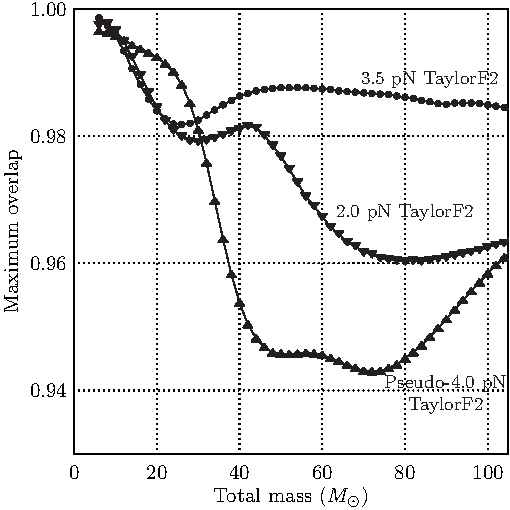
\includegraphics[width=0.5\linewidth]{figures/comparison/ThreeParamOverlapSummaryInitial}
  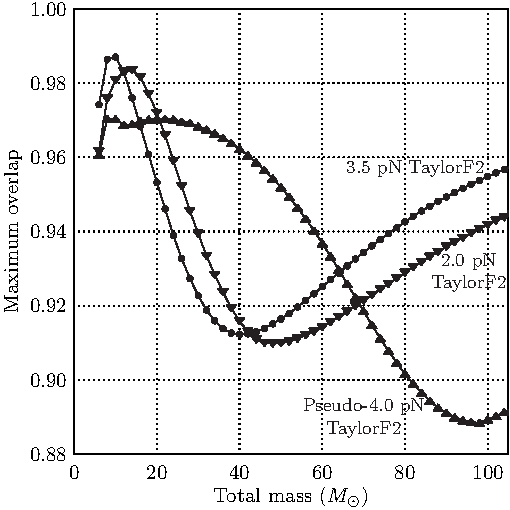
\includegraphics[width=0.5\linewidth]{figures/comparison/ThreeParamOverlapSummaryAdvanced}
  \caption[Overlaps between Caltech--Cornell hybrid waveforms and pN waveforms]{
  \label{fig:ThreeParamOverlapSummaries}
    Left: Overlaps between Caltech--Cornell hybrid waveforms,
    scaled to various masses, and restricted stationary-phase pN
    waveforms for Initial-LIGO PSD. Optimization is over $M$ and
    $\eta$, which the cutoff frequency $f_{c}$ is prescribed by the
    weighted average described below.  The mass ratio $\eta$ is
    allowed to range over unphysical values.  The best-fit values
    found for the pseudo-4.0 pN templates are always physical in this
    case.  See Sec.~\ref{sec:UnrestrictedEta}.  Right: The same, for
    the Advanced-LIGO PSD}
\end{figure}%


\subsection{Effect of upper frequency cutoff}
\label{sec:EffectOfUpperFreqCutoff}

As shown in Fig.~\ref{fig:StildesAndInitialPSD} the amplitude of the
NR waveforms drops sharply at around the lightring frequency, which
depends on the total mass of the binary.  The \textit{TaylorF2}
waveforms do not model the late inspiral, merger or ringdown and hence
will continue to evolve as $f^{-7/6}$ at all frequencies, increasingly
deviating from the NR waveform.  This suggests that the upper
frequency cutoff of the \textit{TaylorF2} waveform should be chosen to
be below the frequency at which the two diverge.  However, the effect
of the divergence is mitigated by the PSD.  The denominator of the
overlap, Eq.~\eqref{eq:OverlapDefinition}, depends on
$\InnerProduct{s|s}$ which is a constant, and $\InnerProduct{h|h}$
which would increase without limit if not for the PSD.
Fig.~\ref{fig:FilterIntegrand} shows $|\tilde{h}(f)|^2/S_n(f)$---the integrand of
$\InnerProduct{h|h}$---for the Initial-LIGO
noise curve for an example \textit{TaylorF2} waveform for an
equal-mass $10\,\MSun$ binary.  We see that above about 450 Hz there
is very little contribution to the integrand, and so extending the
cutoff frequency above this will not impact the overlap.


\begin{figure}
  % \includegraphics[width=\linewidth]{figures/comparison/FilterIntegrand}
  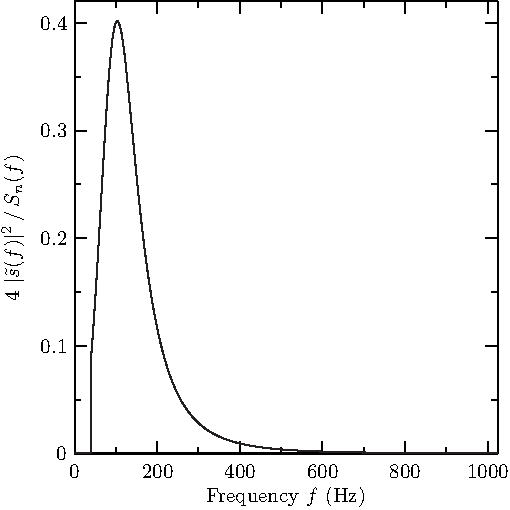
\includegraphics[width=0.50\linewidth]{figures/comparison/Integrand}
  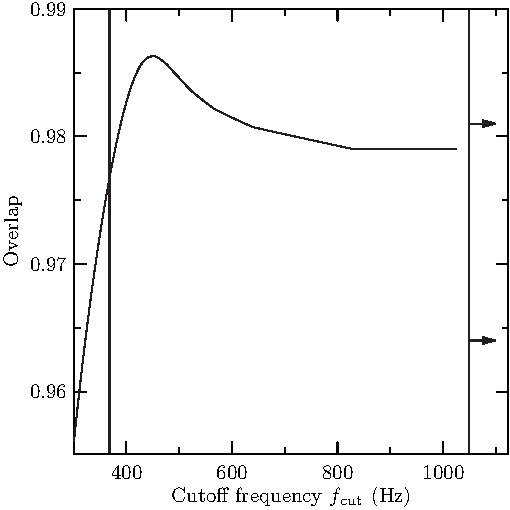
\includegraphics[width=0.50\linewidth]{figures/comparison/Errorbars}
  \caption[Effect of cutoff frequency on overlaps]{
  \label{fig:FilterIntegrand}
    Left: Integrand of Eq.~\eqref{eq:InnerProduct} for a
    \textit{TaylorF2}, 3.5 pN waveform with $M=10$ and $\eta=0.25$, at
    a distance of 100\,Mpc, using the Initial-LIGO noise curve.  Note
    that the shape of this curve does not change as we change $M$ and
    $\eta$; only the vertical scale changes.  Right: Overlap between
    Caltech--Cornell waveform scaled to $M=40\,\MSun$ and restricted
    \textit{TaylorF2}, 3.5 pN waveform using the best-match values for
    $M$ and $\eta$, as a function of the cutoff frequency $f_c$, with
    the Initial-LIGO noise curve.  The vertical bars are meant to
    delineate 1\% loss.  Note that the upper bound extends to higher
    frequencies indefinitely.  }
\end{figure}%


The numerator of the overlap, $\InnerProduct{s|h}$, can only increase
as the cutoff frequency is raised, however frequencies above the
lightring where the waveforms have diverged will contribute very
little.  The effect of including higher frequencies on the overlap is
therefore determined by the $\InnerProduct{h|h}$ term in the
denominator.  For systems with ringdown frequencies well above the
peak of the integrand in Fig.~\ref{fig:FilterIntegrand}, this term
will not significantly reduce the overlap.  For example, binaries of
total mass roughly $40\,\MSun$ have ringdown frequencies at roughly
450\,Hz.  Only a small fraction of the SNR comes from higher
frequencies.  Thus, we expect that systems with lower masses should
not suffer great loss in overlap if the cutoff frequency is higher
than ringdown.  However for higher-mass systems the overlap can be
significantly reduced if the upper frequency cutoff is too large.
This is indeed what we find, as shown by a representative example on
the right in Fig.~\ref{fig:FilterIntegrand}.  For this $40\,\MSun$
system, using the Initial-LIGO noise curve, the optimal cutoff
frequency is around 450\,Hz---roughly the ringdown frequency.
Decreasing the cutoff quickly decreases the overlap.  The cutoff may
be increased almost indefinitely, however, with only 0.5\% loss in
overlap.  This, of course, changes when using the Advanced-LIGO noise
curve.  We revisit this issue in Sec.~\ref{sec:Recommendations}.


\subsection{Unrestricted $\eta$}
\label{sec:UnrestrictedEta}

The physical symmetric mass ratio is restricted to the range $0 < \eta
\leq 0.25$, values above this imply complex-valued masses.  However
the pN waveforms are well-behaved for $0 < \eta < 1.0$, and as seen
from Tables~\ref{tab:ThreeParamOverlapDetailInitial}
and~\ref{tab:ThreeParamOverlapDetail}, the highest overlaps are often
obtained at unphysical values of $\eta$.  In
Fig.~\ref{fig:PhysicalEta} we show the effect of limiting the
optimization to physical $\eta$.  At high masses, the limitation
reduces the optimal overlap by up to 12\%.  \textit{TaylorF2}
waveforms with $\eta \leq 1/4$ would not be expected to accurately
model the late-inspiral and merger part of the waveform, as
non-Newtonian effects are increasingly significant in this region.  We
find that allowing unphysical $\eta$ broadens the space of waveforms
covered by the \textit{TaylorF2} approximation sufficiently to capture
more of the late-inspiral and merger.

\begin{figure}
  % \includegraphics[width=\linewidth]{figures/comparison/PhysicalEta}
  \begin{center}
    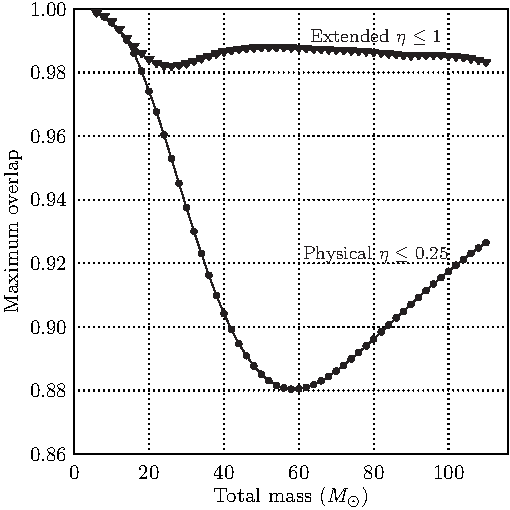
\includegraphics[width=0.55\linewidth]{figures/comparison/PhysicalAndUnphysicalEta}
  \end{center}
  \caption[Maximum overlaps obtained by allowing $\eta$ to range over unphysical values]{
  \label{fig:PhysicalEta}
    Maximum overlaps obtained by allowing $\eta$ to range over
    unphysical values, compared to those obtained by restricting the
    range of $\eta$.  These overlaps are generated using 3.5 pN
    TaylorF2 templates, searching over values of the total mass and
    mass ratio.  Extending to unphysical values of $\eta$ improves the
    match by up to 11\%.}
\end{figure}%


%%%%%%%%%%%%%%%%%%%%%%%%%%%%%%%%%%%%%%%%%%%%%%%%%%%%%%%%%%%%%%%%%%%%%%
%%%%%%%%%%%%%%%%%%%%%%%%%%%%%%%%%%%%%%%%%%%%%%%%%%%%%%%%%%%%%%%%%%%%%%
\section{Recommendations for improvements}
\label{sec:Recommendations} %

Based on the analysis of the previous sections we propose a series of
adjustments to searches using \textit{TaylorF2} template waveforms to
enhance the efficiency of those searches.  First, as seen in
Fig.~\ref{fig:ThreeParamOverlapSummaries} for Initial LIGO, adding
terms up to 3.5 pN order produces overlaps as large or larger than the
current 2.0 pN templates over most of the mass range, while the
pseudo-4.0 pN templates recommended in Ref.~\cite{Pan2007} produce
slightly larger overlaps at masses near $20\,\MSun$.  Thus, we
recommend pseudo-4.0 pN templates for the low mass range, $M < 35
\MSun$, and 3.5 pN templates for higher masses.  The improvement due
to 3.5 pN templates over 2.0 pN generally holds for Advanced LIGO as
well.  The 3.5 pN templates produce larger overlaps than 2.0 pN
templates above $50\,\MSun$ without a significant loss (within 1\%) at
lower masses.  However, there is a large region for which the
pseudo-4.0 pN term does significantly better.  When using an
Advanced-LIGO noise curve, we recommend 3.5 pN templates generally,
2.0 pN templates in the range $12$--$21\,\MSun$ and pseudo-4.0 pN
templates for masses in the range $21$--$65\,\MSun$.

As a second improvement, we note from Fig.~\ref{fig:PhysicalEta} that
allowing $\eta$ to range over unphysical values significantly improves
matches with 3.5 pN templates above $30\,\MSun$. In preliminary
studies we have found that extending to $\eta \leq 1$ roughly doubles
the size of the template bank, and the advantages must therefore be
weighed against the increase in false alarm rate.

\begin{figure}
  % \includegraphics[width=\linewidth]{figures/comparison/FcRecommendationInit}
  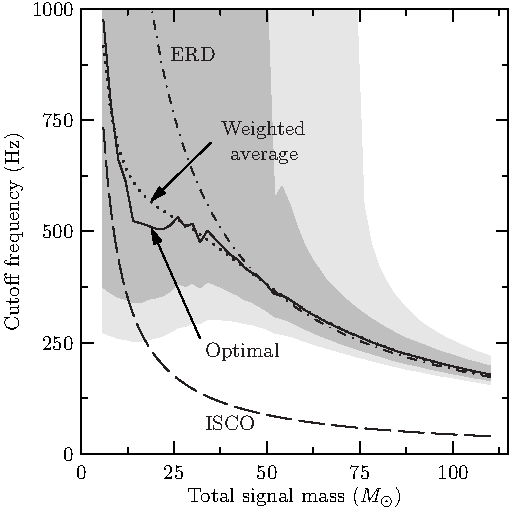
\includegraphics[width=0.5\linewidth]{figures/comparison/FcRecommendationInitial}
  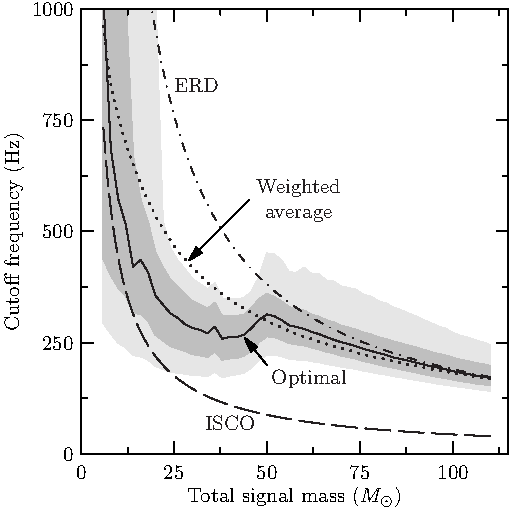
\includegraphics[width=0.5\linewidth]{figures/comparison/FcRecommendationAdvanced}
  \caption[Recommended cutoff frequencies]{
  \label{fig:FcRecomendations}
    Left: Candidate $f_c$ values for 3.5 pN templates with
    Initial LIGO.  The dark gray band contains cutoff frequencies with
    matches within 1\% of the value at which the best overlap was
    obtained.  The light gray band contains frequencies with matches
    within 3\%.  Right: Candidate $f_c$ values for 3.5 pN templates
    with Advanced LIGO.  The dark gray band contains cutoff
    frequencies with matches within 1\% of the value at which the best
    overlap was obtained.  The light gray band contains frequencies
    with matches within 3\%.  Note that the weighted-average cutoff
    extends past the 1\% error bars for $12 < M/\MSun < 40$.  However,
    in that same region, the 3.5 pN templates do poorly overall, and
    we recommend pseudo-4.0 pN templates.  The optimal cutoff
    frequency for pseudo-4.0 pN templates is much closer to the
    weighted-average cutoff in this mass range.}
\end{figure}%

Our third recommendation involves the cutoff frequency used for the
template waveform.  Optimization over the cutoff frequency is too
computationally intensive to be done in searches.  Currently, the
cutoff frequency is typically taken to be the Schwarzschild ISCO
frequency.  To examine the effect of this choice we vary $f_c$ while
keeping the mass and $\eta$ at their optimal values, for each of the
signal masses in our range.  The result of one such variation is shown
in Fig.~\ref{fig:FilterIntegrand} (right).
Figs.~\ref{fig:FcRecomendations} shows the variations for all masses,
highlighting the regions within which the overlap drops by less than
1\% (dark gray) and 3\% (light gray) of the optimal value.  This
figure also shows the ISCO and ERD frequencies, neither of which stays
within the 1\% band for both Initial and Advanced LIGO.  In
particular, the ISCO is a poor choice for both Initial and Advanced
LIGO except at very low masses, where the precise value of the cutoff
is almost irrelevant.

The ISCO is often pointed to---somewhat arbitrarily---as a good
estimate of the breakdown of post-Newtonian
approximations~\cite{Blanchet2006}.  So, for instance, if we were to
match a pN template to a physical waveform, beginning at some point in
the distant past, we might expect them to separate quite badly near
the ISCO.  Of course, for realistic black-hole binaries, the
gravitational waves will only enter the LIGO band late in the
inspiral---just before the ISCO for low-mass systems, or after the
ISCO for high-mass systems.  We can see from
Fig.~\ref{fig:StildesAndInitialPSD} that, for masses below about
$30\,\MSun$, the ISCO is high enough that lower-frequency parts of the
waveform contribute the most to the SNR.  For very high masses,
however, this basically cuts the waveform down to nothing.  In Initial
LIGO, the ISCO is completely buried in seismic noise for masses above
about $100\,\MSun$.  Thus, we must move the cutoff frequency up.  We
cannot push the cutoff far above ringdown, because the physical
waveform simply ceases to exist (see
Fig.~\ref{fig:StildesAndInitialPSD}).  It has been suggested that an
``effective ringdown'' (ERD) frequency $f_{\mathrm{ERD}} \equiv 1.07\,
f_{\mathrm{Ringdown}}$ is a useful upper limit~\cite{Pan2007}.  For
intermediate masses, we would like to interpolate somehow between
these two extremes of ISCO and ERD.  We suggest setting the cutoff
frequency to a weighted average of the two, where the weights are the
contributions to the SNR below the given frequency.  If we assume
coherent phasing between the template and the physical waveform, we
can simply take the amplitudes of the two waveforms.  Also, note that
the restricted SPA approximation for the amplitude is reasonable.
Thus, define
\begin{eqnarray}
  \label{eq:rhoISCO}
  \rho_{\mathrm{ISCO}}^{2} &\equiv & \int_{0}^{f_{\mathrm{ISCO}}}\,
  \frac{f^{-7/3}}{S_{n}(f)}\, d f\ , \\
  \label{eq:rhoERD}
  \rho_{\mathrm{ERD}}^{2} &\equiv & \int_{f_{\mathrm{ISCO}}}^{f_{\mathrm{ERD}}}\,
  \frac{f^{-7/3}}{S_{n}(f)}\, d f\ , \\
  \label{eq:rhoTOT}
  \rho_{\mathrm{tot}}^{2} &\equiv & \int_{0}^{f_{\mathrm{ERD}}}\,
  \frac{f^{-7/3}}{S_{n}(f)}\, d f\ , \\
  \label{eq:fCut}
  f_{\mathrm{cut}} &\equiv & \frac{f_{\mathrm{ISCO}}\ \rho_{\mathrm{ISCO}} +
    f_{\mathrm{ERD}}\ \rho_{\mathrm{ERD}}} {\rho_{\mathrm{tot}}}\ .
\end{eqnarray}
We have already dropped constant factors in the expressions for $\rho$
that will cancel out.

Note that these expressions only depend on the total mass by way of
the limits of integrations---which are very simple, known functions of
the mass---so these integrals could be done just once for a given
noise curve, storing the intermediate values.  When the cutoff needs
to be calculated, the cumulative integral could be evaluated at the
given ISCO and ringdown frequencies.  Hence, this would be a fast way
of calculating the cutoff, with no need to do the integrals each time
the cutoff is needed.

We can test this recommended frequency by comparing it to the optimal
cutoff frequency found by the amoeba search described in
Sec.~\ref{sec:Efficiency}.  For 3.5 pN templates in Initial LIGO, we
find that it is an excellent match to the optimal frequency.
Fig.~\ref{fig:FcRecomendations} shows these two values, along with
dark and light bands showing the regions in which changing $f_{c}$
results in a loss of overlap of 1\% and 3\%, respectively.  Of course,
the same figure shows that using the ERD recommendation would stay
within the 1\% error bounds.  Nonetheless, the close match between
this recommendation and the true optimum suggests that it is sound.
Thus, our final recommendation is to use the weighted-average
frequency cutoff throughout the entire mass range.  While our analysis
has been restricted to equal-mass systems, the cutoff frequency we
have defined here could be applied to unequal-mass systems as well.
It will be interesting to see how this cutoff fares in those
situations.

Similar results hold for Advanced LIGO, when using our recommended
template for each mass.  That is, in regions where 3.5 pN templates do
poorly (see Fig.~\ref{fig:ThreeParamOverlapSummaries}), the weighted
average is a poor predictor of the optimal cutoff frequency using
those templates, as shown in Fig.~\ref{fig:FcRecomendations}.
However, in those same regions---where pseudo-4.0 pN templates do
well---the weighted average is a good predictor of the optimal cutoff
frequency for 4.0 pN templates.  Thus, again, we recommend using the
weighted-average frequency cutoff throughout the entire mass range
with Advanced LIGO.

By prescribing a cutoff frequency, the search does not need to extend
over that parameter.  Similarly, by prescribing a post-Newtonian
order, we need use only one template for a given total mass.  On the
other hand, if these recommendations decrease the overlap found by too
much when using them compared to the overlap found by an unconstrained
search, it may be better to search the larger parameter space.  We can
evaluate the loss in overlap by comparing the results found using our
recommendations to the results found when searching over the set of
all three template families, and all masses, mass ratios, and cutoff
frequencies.  We have determined that this loss in overlap when using
our recommendations is always less than 0.0025 for Initial LIGO, and
less than 0.007 for Advanced LIGO.

\iffalse
\begin{figure}
  \begin{center}
    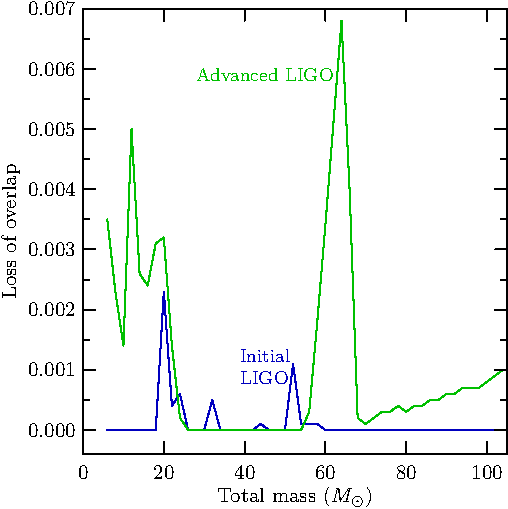
\includegraphics[width=0.55\linewidth]{figures/comparison/WeightedAverageLoss}
  \end{center}
  \caption{Loss in overlap when using our recommendations, compared to
    results searching over all template families, masses, mass ratios,
    and cutoff frequencies.  Our recommendations prescribe the
    template family for a given total mass and the cutoff frequency to
    be used.  In that case, the search is performed for the optimal
    mass and mass ratio of the template.  For Initial LIGO, the loss
    in overlap when using our recommendations is always less than
    0.0025; for Advanced LIGO the loss is always less than 0.007.}
  \label{fig:WeightedAverageLoss}
\end{figure}%
\fi

\section{Conclusions}
\label{sec:Conclusions} %

We have compared high-accuracy NR waveforms for equal-mass binary
black holes from the Caltech--Cornell group to stationary phase
post-Newtonian waveforms.  We examined a number of factors that
influence the matches between the two, with the goal of optimizing the
matches and hence improving the efficiency of templated searches in
Initial and Advanced LIGO.  We first considered the effect of the
post-Newtonian order to which the phase evolution is taken, and found
that adding terms up to 3.5 pN or pseudo-4.0 pN to the currently-used
2.0 pN templates significantly improves the matches over a large range
of masses, as shown in Fig.~\ref{fig:ThreeParamOverlapSummaries}.  We
then studied the effect of varying the upper cutoff frequency of the
templates.  The frequency that achieves the optimal match is a
function of mass, and we find this function is well-approximated by an
average between ISCO and ERD, weighted by contribution to the SNR, as
shown in Fig.~\ref{fig:FcRecomendations}.  Finally, we allow the
symmetric mass ratio $\eta$ to range over unphysical values up to
$1.0$, and find that this dramatically improves matches, as shown in
Fig.~\ref{fig:PhysicalEta}.  Based on the results we recommend
adjusting the searches using \textit{TaylorF2} template waveforms by
going up to 3.5 pN or 4.0 pN over most of the mass range, integrating
up to our recommended cutoff, and allowing allowing $\eta$ to extend
up to 1.  For Initial LIGO, the overlaps obtained using these
parameters is always within 0.0025 of overlaps achievable by
optimizing over all three parameters.

In future work we plan to extend this analysis to unequal-mass and
spinning black-hole systems.  We have found that allowing unphysical
values of $\eta$ roughly doubles the size of the template bank, and we
also plan to study the impact of this on the false alarm rate.




\Chapter{The First NINJA Project}
\label{ch:ninja1}
\newcommand\T{\rule{0pt}{2.6ex}}
\newcommand\B{\rule[-1.2ex]{0pt}{0pt}}
\newcommand\TT{\rule{0pt}{4.2ex}}
\newcommand\BB{\rule[-2.4ex]{0pt}{0pt}}
\newcommand\TTT{\rule{0pt}{3.8ex}}
\newcommand{\Ytwo}{{{}^{-2}Y}}



Thus far, most searches for gravitational waves from BBH mergers have
relied on post-Newtonian results, which are valid when the black holes
are sufficiently far apart.  Within its range of validity,
post-Newtonian theory provides a convenient analytic description of
the expected signals produced by binary systems.  The numerical
relativity results, on the other hand, have not yet been synthesised
into an analytic model for the merger phase covering a broad range of
parameters, i.e., a wide range of mass ratios, spins and if necessary,
eccentricity; there has however been significant progress for the
non-spinning
case~\cite{Buonanno:2006ui,Berti:2007fi,Ajith:2007kx,Pan:2007nw,%
Buonanno:2007pf,Boyle:2007ft,%
Ajith:2007qp,Damour:2007yf,Damour:2007vq,Damour:2008te,Boyle:2008ge,Boyle:2009dg}.
Similarly, despite significant progress, there is not yet a complete
detailed description over the full parameter space of how
post-Newtonian and numerical simulations are to be matched with each
other.  On the data analysis side, many pipelines, especially ones
that rely on a detailed model for the signal waveform, have made a
number of choices based on post-Newtonian results, and it is important
to verify that these choices are sufficiently robust.  More generally,
it is necessary to quantify the performance of these data analysis
pipelines for both detection and parameter estimation.  This is
critical for setting astrophysical upper limits in case no detection
has been made, for following up interesting detection candidates, and
of course for interpreting direct detections. Work on this to date has
primarily used post-Newtonian waveforms. Numerical relativity now
provides an important avenue for extending this to the merger phase.  

There are significant challenges to be overcome before numerical
relativity results can be fully exploited in data-analysis pipelines.
The Numerical INJection Analysis (NINJA) project was started in the
spring of 2008 with the aim of addressing these challenges and
fostering close collaboration between numerical relativists and data
analysts. Participation in NINJA is open to all scientists interested
in numerical simulations and gravitational-wave data analysis.  NINJA
is the first project of its kind that attempts to form a close working
collaboration between the numerical relativity and data analysis
communities.  Several decisions were made that restrict the scope of
the results reported here: we consider only BBH simulations and have
not used results from supernova simulations or simulations containing
neutron stars; the waveform data comes purely from numerical
simulations and we do not attempt to extend numerical data using
post-Newtonian waveforms; the NINJA data set is constructed using
Gaussian noise to model the response of the Initial LIGO and Virgo
detectors -- no attempt has been made to include non-Gaussian noise
transients found in real detector data.  The comparisons and
conclusions reported here are thus necessarily limited, and in many
cases are only the first steps towards fully understanding the
sensitivity of data-analysis pipelines to black hole signals.  Further
studies are needed regarding the accuracy and comparison of numerical
waveforms, and of how systematic errors in these waveforms can affect
parameter estimation.  Some analyses of numerical waveforms with
regard to gravitational-wave detection have already been
performed~\cite{Baumgarte:2006en,Vaishnav:2007nm,Pan:2007nw,Boyle:2009dg},
accuracy standards have been developed for use of numerical waveforms
in data analysis~\cite{Lindblom:2008cm} and a detailed comparison of
some of the waveforms used in the NINJA project was performed in the
related Samurai project~\cite{Hannam:2009hh}.  We expect that
subsequent NINJA analyses will build on these results to address these
issues.  

Despite the limited scope of the first NINJA project, we are able to
draw the following broad conclusions from this work.  Our first
conclusion is that the current data analysis pipelines used to search
LIGO, Virgo and GEO600 data for black hole coalescence are able to
detect numerical waveforms injected into the NINJA data set at the
expected sensitivities. Indeed, several of these pipelines are able to
detect signals that lie outside the parameter space that they target.
This is a non-trivial statement since most detectability estimates to
date for these sources have relied on post-Newtonian waveforms, which
are valid only when the black holes are sufficiently far apart. For
many of these pipelines, this is the first time they have been tested
against numerical waveforms. It should be noted, however, that the
NINJA data set does not contain non-stationary noise transients so
more work is needed to understand how detection performance is
affected by the noise artifacts seen in real gravitational-wave
detector data. Our second conclusion is that significant work is
required to understand and improve the measurement of signal
parameters.  For instance, among the pipelines used in this first
NINJA analysis only the Markov-chain Monte-Carlo algorithm attempted
to estimate the spins of the individual black holes, and the
estimation of the component masses by the detection pipelines is poor
in most cases.  Improvement in this area will be crucial for bridging
the gap between gravitational wave observations and astrophysics.
NINJA has proven to be extremely valuable at framing the questions
that need to be answered.

% end introduction.tex

\section{Numerical Waveforms}
\label{sec:ninja1_nrwaveforms}
%begin nrwaveforms.tex

The NINJA project has studied BBH coalescence waveforms submitted by
ten individuals and teams.  Participation in NINJA was open to anyone
and the only restrictions were that each contribution: (i) was a
numerical solution of the full Einstein equations, (ii) consisted of
only two waveforms, or up to five waveforms if they were part of a
one-parameter family.

No restrictions were placed on the accuracy of each waveform. All
contributions followed the format specified in~\cite{Brown:2007jx}.
The waveforms are plotted in Figures~\ref{fig:NR-Reh22} and
\ref{fig:NR-SumAllModes}.
%
The contributed waveforms cover a variety of physical and numerical
parameters. Most simulations model low-eccentricity inspiral, the mass
ratio $q = m_1/m_2$ ranges from 1 to 4, and the simulations cover a
range of spin configurations.  The initial angular frequency of the
$\ell=m=2$ mode ranges from $0.033/M$ to $0.203/M$ (where $M$ denotes
the sum of the initial black-hole masses). This initial angular
frequency marks where contributors consider the waveform sufficiently
clean to represent the physical system (e.g. this will be chosen after
initial unphysical radiation content, often referred to as ``junk
radiation'' in numerical relativity, is radiated away).   The length
of the waveforms varies between a few 100M to over 4000M.  The
contributions naturally differ in accuracy, both regarding how well
they capture the black-hole dynamics and in the extraction of the
gravitational-wave signal. 

Table~\ref{tab:allwaveforms} lists a few key parameters that
distinguish the waveforms, and introduces the following tags for the
different contributions and codes:
%
% XXX This is the paragraph that people should copy to get the NINJA NR refs
%
BAM~HHB~\cite{Brugmann:2008zz,Husa:2007hp,Hannam:2007ik,Hannam:2007wf,Bruegmann:2003aw} 
and BAM~FAU~\cite{Brugmann:2008zz,Husa:2007hp,Tichy:2008du,Bruegmann:2003aw}
are contributions using the {\tt BAM} code,
{\tt CCATIE} is the AEI/LSU code~\cite{Alcubierre:2000xu,Alcubierre:2002kk,Koppitz:2007ev,Pollney:2007ss,Rezzolla:2007xa},
{\tt Hahndol} is the Goddard Space Flight Center's code~\cite{Imbiriba:2004tp,vanMeter:2006vi}, 
{\tt LazEv} is the RIT code~\cite{Zlochower:2005bj,Campanelli:2005dd,Dain:2008ck}, 
{\tt Lean} is Ulrich Sperhake's code~\cite{Sperhake:2006cy,Sperhake:2007gu,Sperhake:2008ga}, 
{\tt MayaKranc} is the Georgia Tech/Penn State code~\cite{Vaishnav:2007nm,Hinder:2007qu}, 
PU stands for the Princeton University code~\cite{Pretorius:2004jg,Pretorius:2005gq,Buonanno:2006ui,Pretorius:2007jn},
{\tt SpEC} for the Cornell/Caltech collaboration 
code~\cite{Scheel:2006gg,Pfeiffer:2007yz,Boyle:2007ft,Scheel:2008rj},
and
{\tt UIUC} stands for the University of Illinois at
Urbana-Champaign team~\cite{Etienne:2007hr}.

The codes listed above use different formulations of the Einstein
equations, gauge conditions, mesh structures, initial data and wave
extraction methods; we will attempt to give a unified presentation of
common features first, and then list further details of the approaches
separately for each contribution. Full details of each code are given
in the references.
%More detailed descriptions of each contribution are posted on the
%NINJA project web pages [REF], and full details of each code are
%given in the references. {\bf Currently the write-ups are not
%accessible to non-Ninjas.}

The numerical codes follow either of two approaches to solving the
Einstein equations: (1) the generalised harmonic formulation, which
was the basis of Pretorius' initial breakthrough simulation of
coalescing black holes \cite{Pretorius:2005gq}, or (2) the
moving-puncture approach, following
\cite{Campanelli:2005dd,Baker:2005vv}.  Both approaches result in
canonical choices for the construction of initial data, the evolution
system for the Einstein equations, and the treatment of the
singularity inside the black-hole horizons.

\begin{table}
\begin{center}
\begin{tabular}{|l|l|l|l|l|l|c|c|}\hline
Code & Run & $q$ & $\vec S_i/m_i^2$ & $e$ & $\omega_{22}\, M$ & $D/M$ &
eccentricity
\\ 
\hfill Ref.     &     &   &                        &   &          &       &
     removal \\ \hline

BAM~FAU      & \cite{Tichy:2008du}       & 1 & 
%$\vec\chi_1^{\rm FAU}$,  $\vec\chi_2^{\rm FAU}$  
see caption
& qc  & 0.06 & $9.58\,\hat y$ & T-PN \cite{Marronetti:2007ya,Marronetti:2007wz} \\
\hfill\cite{Brugmann:2008zz,Husa:2007hp}              &        &   &
&    &      & &   \\[1em]

BAM~HHB      & S00 \cite{Hannam:2007ik}   & 1 & $0$       & $< 0.002$   &
0.045 & $12\,\hat y$ & TR-PN \cite{Husa:2007rh} \\ 
\hfill\cite{Brugmann:2008zz,Husa:2007hp}              & S25 \cite{Hannam:2007wf}   & 1 & $0.25\,\hat z$    & $\approx 0.006$  &
              0.045 & $12\,\hat y$ & T-PN \cite{Brugmann:2007zj} \\
              & S50 \cite{Hannam:2007wf}   & 1 & $0.50\,\hat z$    & $\approx 0.006$  &
              0.052 & $11\,\hat y$ & -- '' -- \\ %T-PN \cite{Brugmann:2007zj} \\
              & S75 \cite{Hannam:2007wf}   & 1 & $0.75\,\hat z$    & $\approx 0.006$ &
              0.06 &  $10\,\hat y$ & -- '' -- \\ %T-PN \cite{Brugmann:2007zj} \\
              & S85 \cite{Hannam:2007wf}   & 1 & $0.85\,\hat z$    & $\approx 0.006$  &
              0.06 &  $10\,\hat y$ & -- '' -- \\[1em] %T-PN
                                %\cite{Brugmann:2007zj} \\


{\tt CCATIE}
              & r0~\cite{Pollney:2007ss}    & 1 & $0.6\,\hat z$, $-0.6\,\hat z$  & qc &
              0.079 & $8\,\hat x$ & TR-PN \cite{Husa:2007rh} \\
\hfill\cite{Alcubierre:2000xu,Alcubierre:2002kk,Koppitz:2007ev,Pollney:2007ss}
	      & r2~\cite{Pollney:2007ss}     & 1 & $0.6\,\hat z$, $-0.3\,\hat z$    & qc  &
              0.078 & $8\,\hat x$ & -- '' -- \\ %TR-PN \cite{Husa:2007rh} \\
              & r4~\cite{Pollney:2007ss}     & 1 & $0.6\,\hat z$, $0$       & qc  &
              0.076 & $8\,\hat x$ & -- '' -- \\ %TR-PN \cite{Husa:2007rh} \\
              & r6~\cite{Pollney:2007ss}     & 1 & $0.6\,\hat z$, $0.3\,\hat z$    & qc  &
              0.075 & $8\,\hat x$ & -- '' -- \\%TR-PN \cite{Husa:2007rh} \\
              & s6~\cite{Rezzolla:2007xa}     & 1 & $0.6\,\hat z$     & qc  &
              0.074 & $8\,\hat x$ & -- '' -- \\[1em] %TR-PN \cite{Husa:2007rh} \\ 

{\tt Hahndol}      & kick   & 3 & $0.2\,\hat x$, $0.022\,\hat x$ & qc  &0.078 &  $8.007\,\hat{y}$ & T-PN \cite{Kidder:1995zr}\\ 
\hfill\cite{Imbiriba:2004tp,vanMeter:2006vi}            & non    & 4 & $0$     & qc
              &0.070 & $8.470\,\hat{y}$ & -- '' -- \\ %T-PN \cite{Kidder:1995zr} \\

{\tt LazEv}$\,$\cite{Zlochower:2005bj,Campanelli:2005dd}$\!$    & MH~\cite{Dain:2008ck} & 1 & $0.92\,\hat z$   & qc  &
0.07  & $8.16\,\hat x$ & T-PN \cite{Kidder:1995zr,Blanchet:1999pm} \\[1em]

{\tt Lean}\hfill\cite{Sperhake:2006cy}      &  c     & 4 & $0$       & qc  &
0.05  & $10.93\,\hat x$ & T-PN \cite{Brugmann:2008zz} \\ 
             &  2     & 1 & $0.926\,\hat z$   & qc  &
              0.11  & $6.02\,\hat x$ & T-PN \cite{Kidder:1995zr} \\[1em]

{\tt MayaKranc}     & e0  \cite{Hinder:2007qu}   & 1 & $0$       &  qc &
0.05 & $12\,\hat x$ & TR-PN \cite{Husa:2007rh} \\
  \hfill\cite{Vaishnav:2007nm}            & e02 \cite{Hinder:2007qu}   & 1 & $0$       & 0.2&
              0.05 & $15.26\,\hat x$ & n/a \\[1em]

PU\hfill\cite{Pretorius:2004jg,Pretorius:2005gq}  & CP \cite{Buonanno:2006ui}    & 1 & $0.063\,\hat z$      & qc  &
0.07  & $9.5\,\hat x$ & T-ID \cite{Cook:2004kt} \\
              & T52W \cite{Pretorius:2007jn}  & 1 & $0$       & $\ge
              0.5$ & 0.07 & & n/a \\[1em]

{\tt SpEC}\hfill  \cite{Scheel:2006gg}        & q=1 \cite{Boyle:2007ft,Scheel:2008rj}       & 1 & $0$       & $5\times 10^{-5}$  &
0.033 & $15\,\hat x$ & TR-it \cite{Pfeiffer:2007yz} \\[1em]

UIUC \hfill\cite{Etienne:2007hr}          & cp \cite{Etienne:2007hr}     & 1 & $0$       & qc  &
0.194 & $4.790\,\hat x$ & T-ID \cite{Cook:2004kt} \\ 
             & punc \cite{Etienne:2007hr}   & 1 & $0$     & qc  &
              0.203 & $4.369\,\hat y$ & T-ID \cite{Tichy:2003qi} \\  \hline
\end{tabular}
\end{center}
\caption{{\bf Initial conditions for numerical waveforms.}
The columns list, in order from left
to right, the name of the contribution or code, the name of the run
where appropriate, 
the mass ratio $q=m_1/m_2$ where $m_1\ge m_2$, the
spins of the black holes in vector form (if only one spin is given, both spins are equal), an estimate of the initial
eccentricity of the orbit (the entry qc denotes cases where quasi-circular inspiral, i.e.~zero eccentricity
is modelled, but a value of the eccentricity has not been reported), the initial frequency of the $(\ell,m)=(2,2)$
mode (rounded to three digits), the initial coordinate separation
of either the black-hole punctures or the excision surfaces, and where
appropriate the method of eccentricity removal.  All binaries start
out in the $xy$-plane with initial momenta tangent to the $xy$-plane.  See text for the
identification of each contribution, and a description of the notation
in the last column. 
The dimensionless spins of the BAM~FAU run are $(-0.634,-0.223, 0.333)$ and 
$(-0.517,-0.542,0.034)$.}
\label{tab:allwaveforms}
\end{table}



\begin{table}
\begin{center}
\begin{tabular}{|l|l|c||c|c|c|}\hline
Code & Run & q % & $\vec S_i/m_i^2$ & e & $\omega_{22}\, M$ 
& $\Delta T_{\rm 100}$ [s] & $f_{i,\rm 100}$ [Hz] & $M_{30 Hz} [M_\odot]$ \\ %& ${\cal M}_{30 Hz} [M_\odot]$
 \hline

BAM~HHB    & S00  & 1 % & $0$                   & $< 0.002$ & 0.045 
& 1.03 & 15 & 48  \\ %& 21 \\ 
            & S25  & 1 % & $0.25\hat z$  & $\approx 0.006$  & 0.045 
& 1.15 & 15 & 48  \\ %& 21 \\
            & S50  & 1 % & $0.50\hat z$  & $\approx 0.006$  & 0.052 
& 1.03 & 17 & 56  \\ %& 24 \\
            & S75  & 1 % & $0.75\hat z$  & $\approx 0.006$  & 0.06  
& 0.81 & 19 & 65  \\ %& 28 \\
            & S85  & 1 % & $0.85\hat z$  & $\approx 0.006$  & 0.06  
& 0.87 & 19 & 65  \\ %& 28 \\

BAM~FAU    &      & 1 % & see caption                   & qc & 0.06  
& 0.54 & 19 & 65  \\ %& 28 \\ 

{\tt CCATIE}& r0   & 1 % & $0.6\hat z$, $-0.6\hat z$ & qc & 0.079 
& 0.34 & 26 & 85  \\ %& 37\\
            & r2   & 1 % & $0.6\hat z$, $-0.3\hat z$ & qc & 0.078 
& 0.37 & 25 & 84  \\ %& 37 \\
            & r4   & 1 % & $0.6\hat z$, $0$            & qc & 0.076 
& 0.40 & 25 & 82  \\ %& 36 \\
            & r6   & 1 % & $0.6\hat z$, $0.3\hat z$  & qc & 0.075 
& 0.45 & 24 & 81  \\ %& 35 \\
            & s6   & 1 % & $0.6\hat z$                 & qc & 0.074 
& 0.59 & 24 & 80  \\ %& 35 \\

{\tt Hahndol}&kick & 3 % & $0.2\hat x$, $0.022\hat x$& qc & 0.078 
& 0.25 & 25 & 84  \\ %& 31 \\
            & non  & 4 % & $0$                           & qc & 0.070 
& 0.32 & 23 & 75  \\ %& 25 \\

{\tt LazEv} & MH   & 1 % & $0.92\hat z$                & qc & 0.07  
& 0.43 & 23 & 75  \\ %& 33 \\

{\tt Lean}  &  c   & 4 % & $0$                           & qc & 0.05  
& 0.92 & 16 & 54  \\ %& 18 \\
            &  2   & 1 % & $0.926\hat z$               & qc & 0.11  
& 0.20 & 36 & 118\,\,\,  \\ %& 52 \\

{\tt MayaKranc}& e0& 1 % & $0$                           & qc & 0.05  
& 1.23 & 16 & 54  \\ %& 23 \\
            & e02  & 1 % & $0$                          & 0.2 & 0.05  
& 0.74 & 16 & 54  \\ %& 23 \\

PU          & CP   & 1 % & $0.063\hat z$               & qc & 0.07  
& 0.29 & 23 & 75  \\ %& 33 \\
            & T52W & 1 % & $0$                   & $\ge  0.5$ & 0.07  
& 0.16 & 23 & 75  \\ %& 33 \\

{\tt SpEC}  & q=1  & 1 % & $0$                   & $<10^{-5}$  & 0.033 
& 1.96 & 11 & 36  \\ %& 15 \\

UIUC        & cp   & 1 % & $0$                           & qc & 0.194 
& 0.10 & 63 & 209\,\,\,  \\ %& 91 \\
            & punc & 1 % & $0$                           & qc & 0.203 
& 0.10 & 66 & 219\,\,\,  \\ %& 95 \\

 \hline
\end{tabular}
\end{center}
\caption{\label{tab:allwaveforms-SI}%
{\bf Characteristic duration, mass and frequencies} of
the waveforms summarised in table~\ref{tab:allwaveforms}.
The columns $\Delta T_{\rm 100}$ and $f_{i, 100}$ give the duration and initial
frequency of the waveform when scaled to total mass $M=100M_{\odot}$.
$M_{30Hz}$ is the total mass of the waveform when it is scaled so that
the initial frequency is 30Hz (this sets the lowest mass at which each waveform  can be injected into the NINJA data).  }
\end{table}



%%%%%%%%%%%%%%%%%%%%%%%%%%%%%%%%%%%%%%%%%%%%%%%%%%%%%%%%%%%%%%%%

\begin{figure}
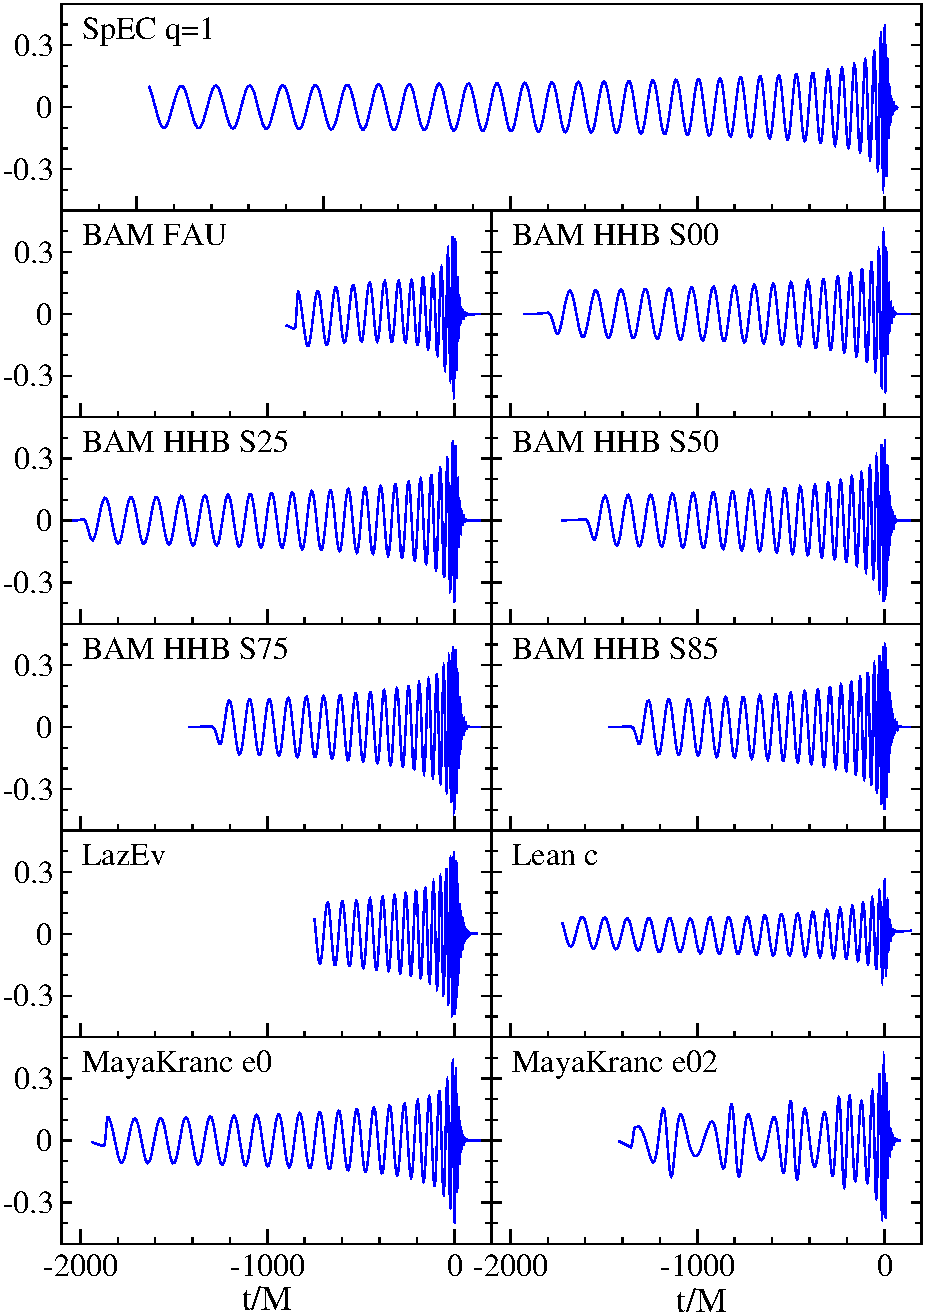
\includegraphics[width=0.49\textwidth]{figures/ninja1/Prune_Re_h22-A}
$\;$
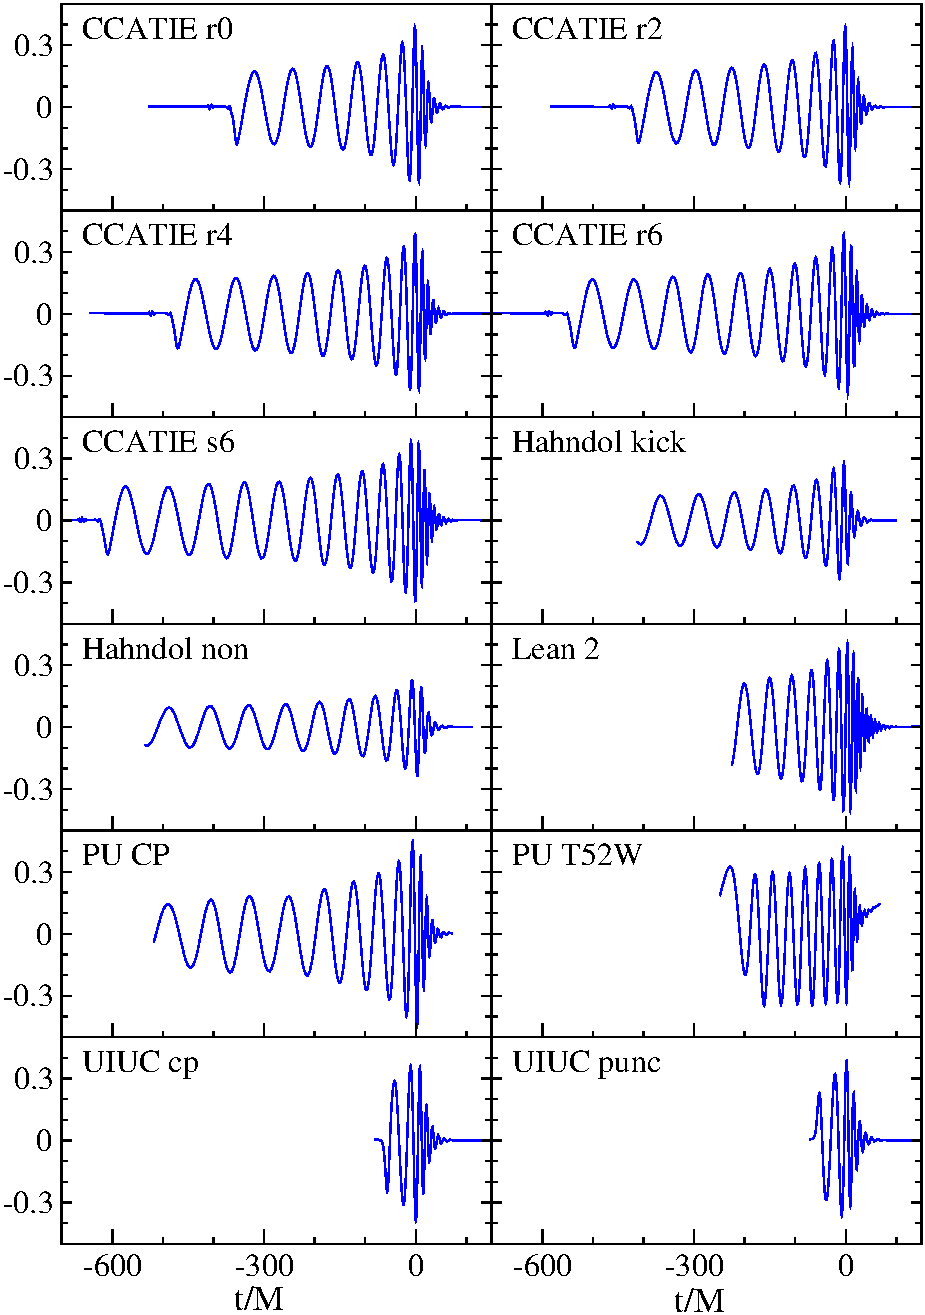
\includegraphics[width=0.49\textwidth]{figures/ninja1/Prune_Re_h22-B}\\[-.25em]

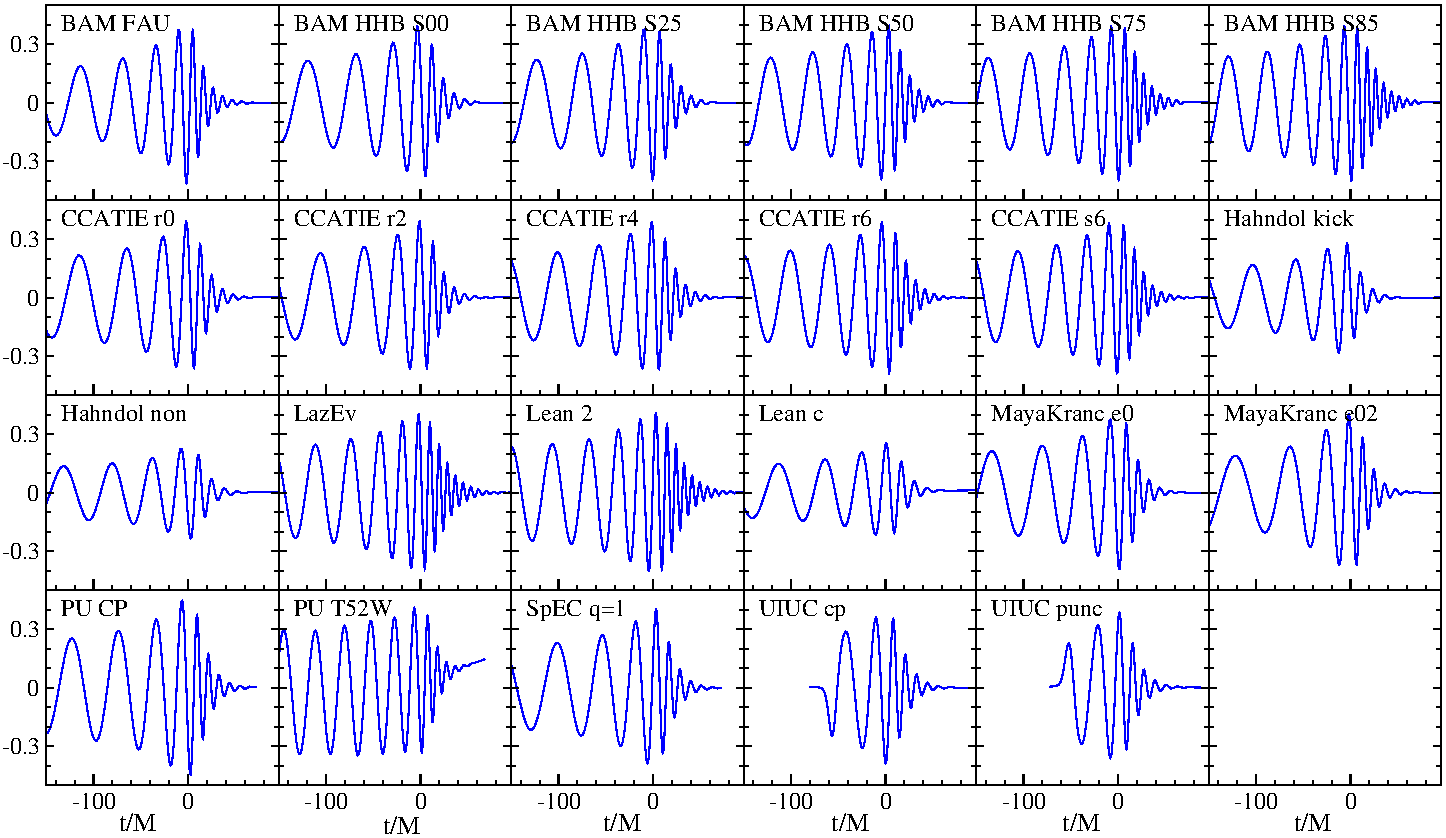
\includegraphics[width=\textwidth]{figures/ninja1/Prune_Re_h22-Merger}

\caption[Summary of waveforms contributed to NINJA1]]{
\label{fig:NR-Reh22} Summary of all submitted numerical waveforms: \boldmath$r/M\,\mbox{Re}(h_{22})$ 
The $x$-axis shows time in units of $M$ and the $y$-axis shows the 
real part of the $(\ell,m)=(2,2)$
  component of the dimensionless wave strain $r h = r h_+ - i r
  h_\times$.
  The top panels show the complete
  waveforms: the top-left panel includes waveforms that last more
  than about $700M$, and the top-right panel includes waveforms
  shorter than about $700M$. The bottom panel shows an enlargement of
  the merger phase for all waveforms.}
\end{figure}


\begin{figure}
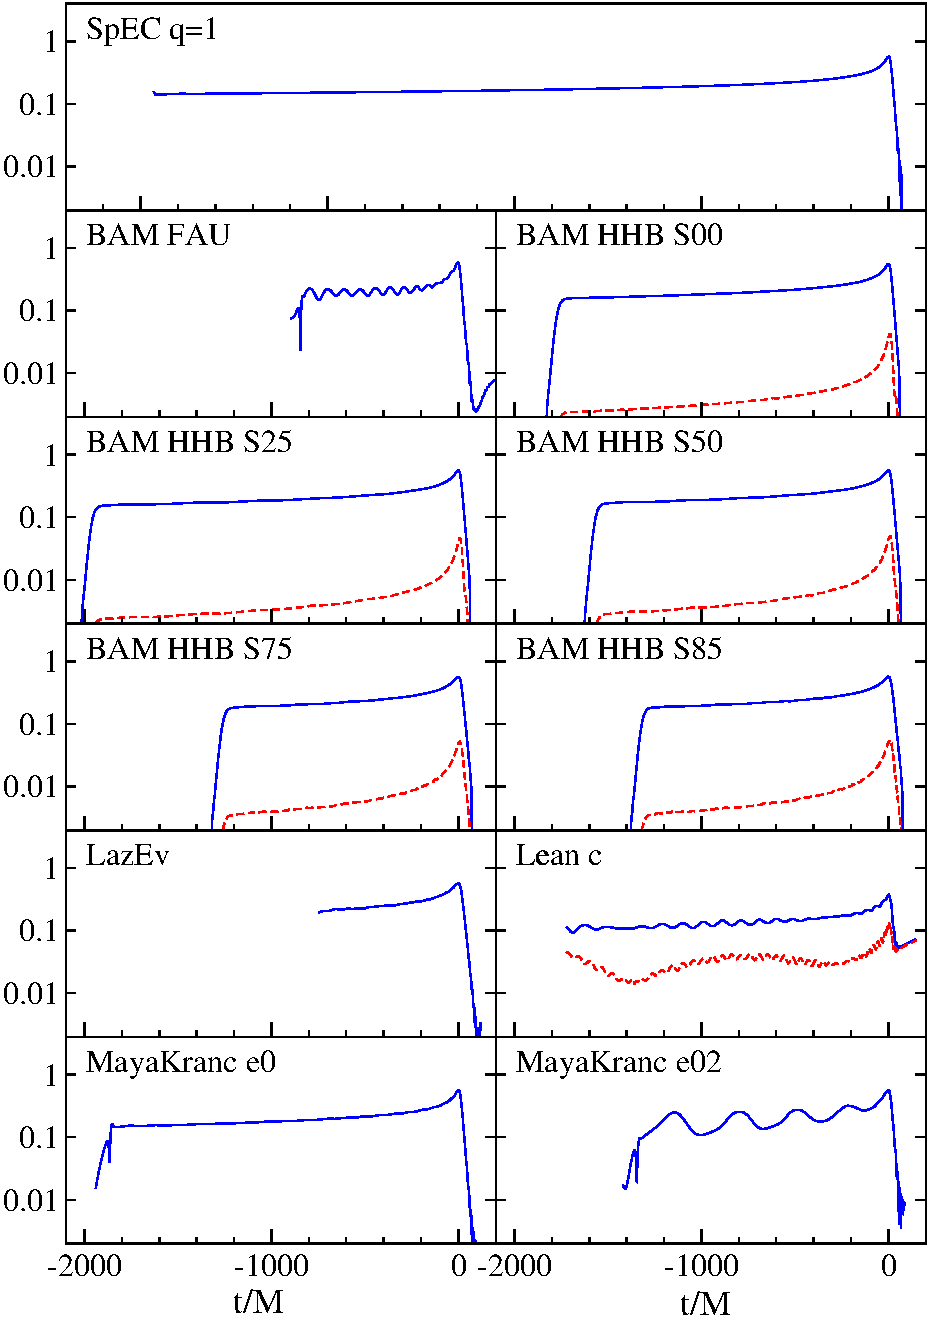
\includegraphics[width=0.49\textwidth]{figures/ninja1/Prune_SumAllModes-A}
$\;$
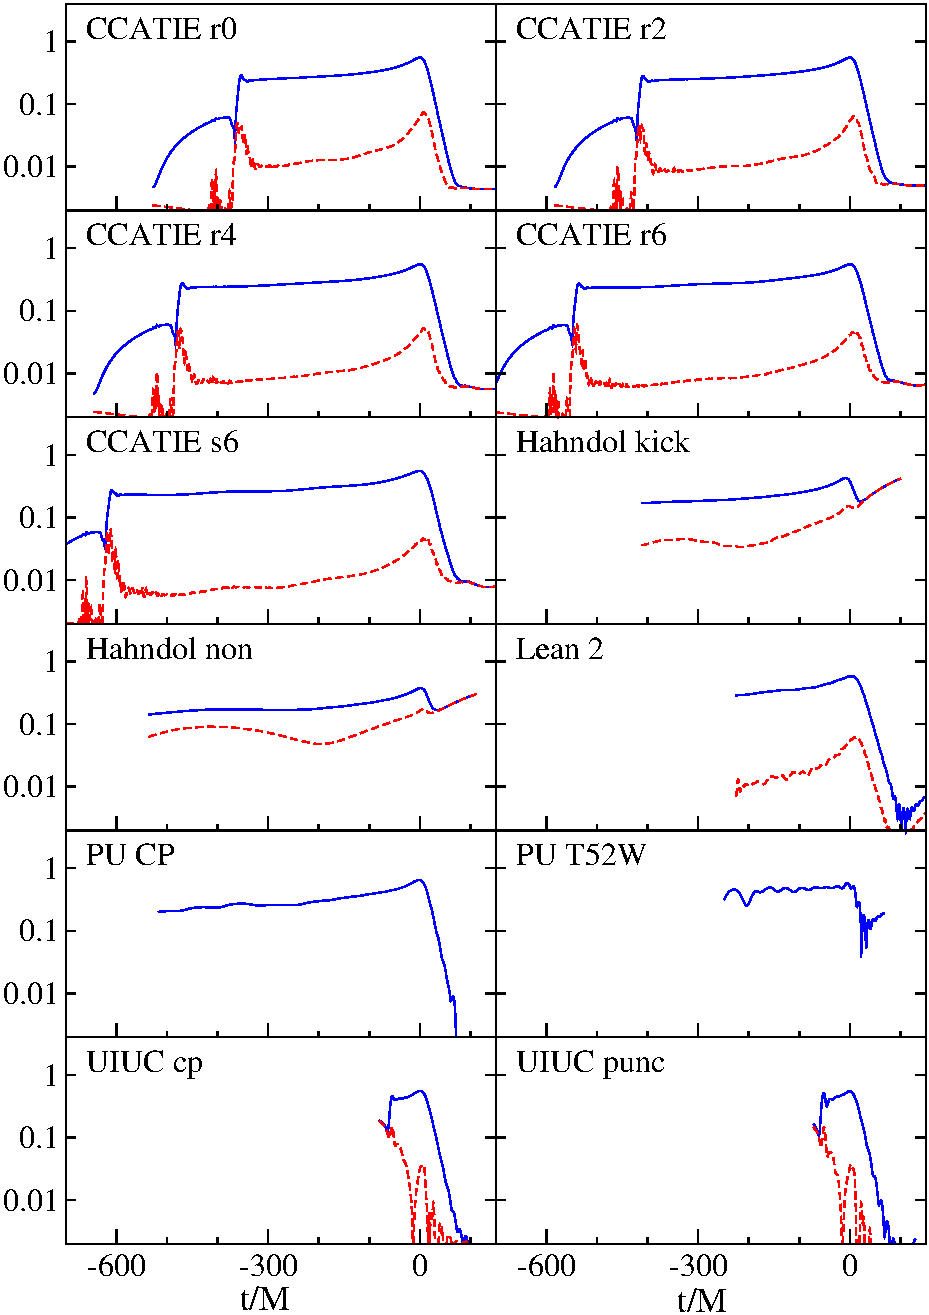
\includegraphics[width=0.49\textwidth]{figures/ninja1/Prune_SumAllModes-B}\\[-0.25em]

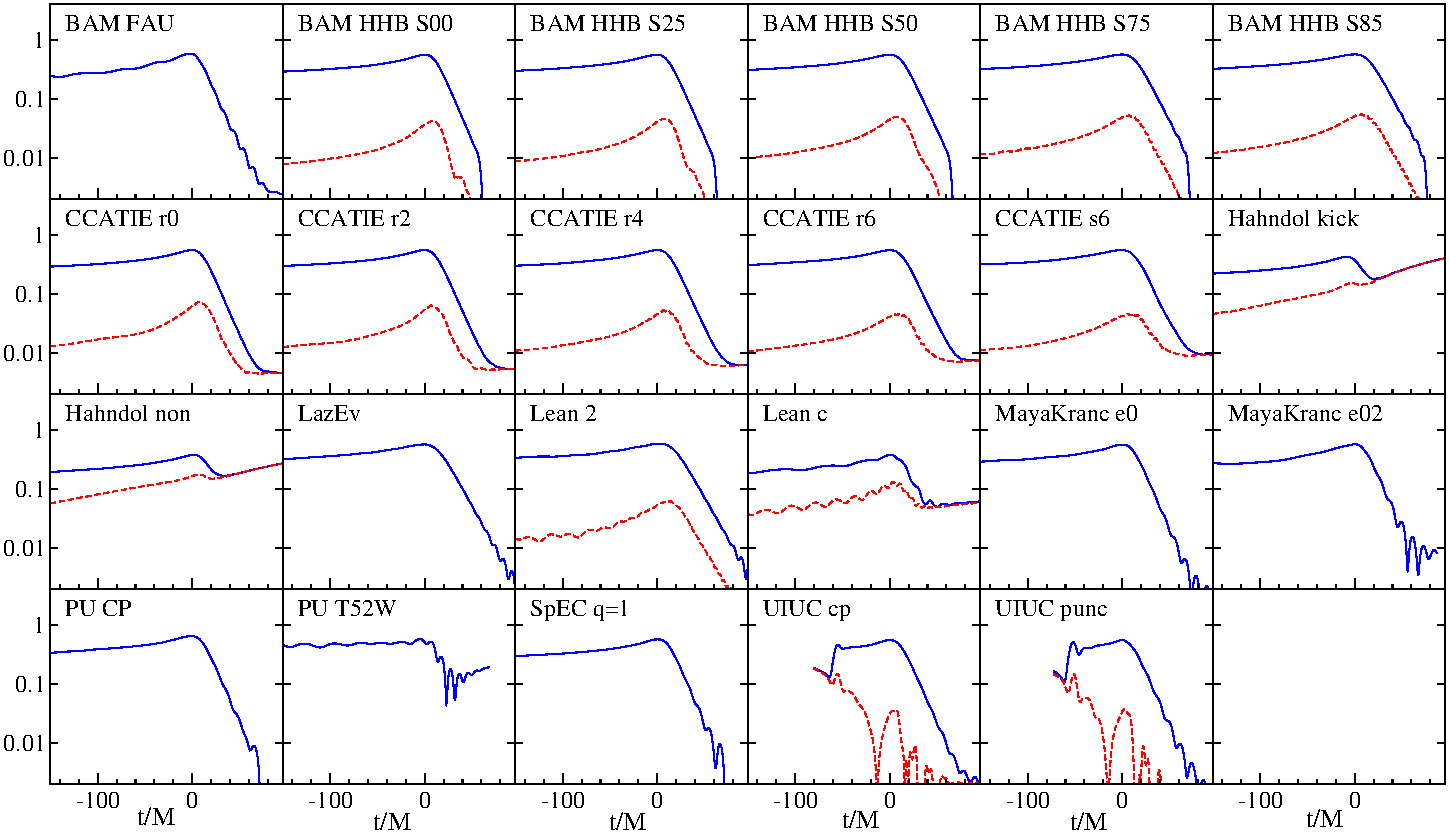
\includegraphics[width=\textwidth]{figures/ninja1/Prune_SumAllModes-Merger}

\caption[Distribution of power into different spherical harmonics]{
\label{fig:NR-SumAllModes}
Distribution of power into different spherical harmonics.  The blue line shows
  $\left(\Sigma_{\ell,m}|h_{\ell m}\,r/M|^2\right)^{1/2}$.  A dashed red line, if
  present, shows the same sum, but {\em excluding} the $(\ell,m)=(2,\pm
  2)$ modes. 
  The separation between the two lines gives the relative importance
  of non $(2,\pm 2)$ modes.  If no red line is present for a certain
  run, then only the $(2,\pm 2)$ modes were supplied.  The layout is
  as in Fig.~\ref{fig:NR-Reh22}: The top panels show the complete
  waveforms, whereas the bottom panel shows an enlargement of the
  merger phase. The $x$-axis shows time in units of $M$.
}
\end{figure}


%%%%%%%%%%%%%%%%%%%%%%%%%%%%%%%%%%%%%%%%%%%%%%%%%%%%%%%%%%%%%%%%%%%%%%%


%%%%%%%%%%%%%%%%%%%%%%%%%%%%%%%%%%%%%%%%%%%%%%%%%%%%%%%%%%%%%%%%%%%%%%%
\subsection{Summary of the simulation algorithms}
\label{ssec:sumalg}

%%%%%%%%%%%%%%%%%%%%%%%%%%%%%%%%%%%%%%%%%%%%%%%%%%%%%%%%%%%%%%%%%%%%%%%
\subsubsection{Initial Data}
\label{ssec:id}

Due to the presence of constraint equations, specifying initial data
in numerical relativity is far from trivial, for a general overview
see e.g.~\cite{Cook:2000vr}.  All of the results presented here make
the simplifying assumption of conformal flatness for the spatial
metric of the initial slice, which leads to some spurious
gravitational radiation in the initial data.  All contributions
attempt to model non-eccentric inspiral, except for the two data sets
PU--T52W and {\tt MayaKranc}--e02.  However, the degree of
``quasi-circularity'' varies, and in general one should bear in mind
that the definition of eccentricity for fully general-relativistic
orbits is not unique (see for
example~\cite{Sperhake:2007gu,Hinder:2007qu}).   The data set PU--T52W
is notable for the fact that the BBH was constructed via scalar field
collapse. Specifically, the initial data consists of two, compact,
dense distributions of scalar field energy, separated by some distance
and Lorentz boosted in opposite directions orthogonal to the line
between them. Upon subsequent evolution, each scalar field pulse
quickly collapses to form a black hole, with all remnant scalar field
energy radiating away from the domain on the order of the
light-crossing time of the orbit. This is the same time scale on which
spurious gravitational radiation present in all current initial-data
sets leaves the domain of the inspiral, and hence for practical
purposes this can be considered a vacuum merger.  All other runs start
from vacuum initial data. 

Most codes ({\tt BAM}, {\tt CCATIE}, {\tt Hahndol}, {\tt LazEv}, {\tt
Lean}, {\tt MayaKranc} and the UIUC code) adopt the ``moving
puncture'' approach, following \cite{Campanelli:2005dd,Baker:2005vv}.
These codes use puncture initial data
\cite{Bowen:1980yu,Beig:1993gt,Brandt:1997tf} to model black holes,
resulting in initial data that contain a separate asymptotically flat
end within each black hole.  Constructing such initial data is
mathematically well understood~\cite{Beig:1993gt,Dain:2001ry}. 
% I think the next sentence is misleading, if you really want to have
% it in, contact me please - Sascha.  and for simple cases the
% evolution of such initial data has been shown to be equivalent to
% that of excised black holes~\cite{Thornburg:2007hu}.
The codes {\tt CCATIE}, {\tt LazEv}, {\tt Lean} and {\tt MayaKranc}
all use the same pseudo-spectral solver for the Einstein constraint
equations~\cite{Ansorg:2004ds}, and {\tt BAM} uses a variant
thereof~\cite{Husa:2007hp}.  {\tt UIUC-punc} initial data is generated
via the \textsc{Lorene} \cite{Lorene} multi-domain spectral libraries.
The {\tt Hahndol} code uses the second-order-accurate multi-grid
solver \textsc{amrmg} \cite{Brown:2004ma}, which is however tuned to
give truncation errors typically much smaller than those produced by
the evolution code.

The generalised harmonic codes use conformal thin sandwich initial
data~\cite{York:1998hy}.  PU-CP and {\tt SpEC} use quasi-equilibrium
excision initial data  where the interior of the black-hole horizons
has been excised from the numerical grid. The presence of black holes
with desired linear momenta and spins is enforced through the boundary
conditions on the excision surfaces and the numerical outer boundary
during the solution of the initial-value equations
\cite{Cook:2001wi,Cook:2004kt,Caudill:2006hw,Pfeiffer:2007yz}. This
``excision technique'' is based on the defining property of black
holes --- the horizons act as causal membranes and information cannot
escape from the inside.  The {\tt UIUC-cp} simulation uses the same
excised initial data, but fills the BH interior with ``smooth junk'',
as described in~\cite{Etienne:2007hr}, before evolving with the moving
puncture technique.   
% This is a repeat of the material above:
%PU--T52W uses initial data in which black holes are formed by scalar
%field collapse. 

All codes take input parameters that ultimately determine the
individual black-hole masses $m_i$, spins $\vec{S}_i$, momenta
$\vec{P}_i$ and coordinate separation $D$ of the black holes (one
should however be aware that in the strong field regime of general
relativity various subtleties are associated with the definition of
all of these quantities). In addition, the black-hole masses and
dimensionless spins slowly change during the inspiral, which requires
additional caution regarding the definition and accuracy of the values
of mass, spin, etc.  There are two common methods to estimate the
instantaneous individual black-hole masses. One is to calculate the
\emph{apparent-horizon mass}, computed from the irreducible mass
(given by the area of each hole's horizon) and the spin according to
Christodoulou's \cite{Christodoulou:1970wf} relation $m_i^2 =
m_{i{\rm,irr}}^2 + S_i^2/(4 m_{i,{\rm irr}}^2)$. The other, applicable
only to puncture data, is to compute the Arnowitt-Deser-Misner (ADM)
mass~\cite{Arnowitt1962} at each puncture, which corresponds to
spatial infinity in a space that contains only that black
hole~\cite{Brandt:1997tf}. We generally use the total black-hole mass
$M=m_1+m_2$ to scale dimensionful quantities, although sometimes the
total conserved energy ($M_\mathrm{ADM}$) is used for this purpose. 
%
% There are essentially two different approaches to quoting
% mass-related parameters of the black holes. One approach (e.g.\
% Goddard) is to assume that all the Bowen-York spin is ultimately
% absorbed by its puncture (this usually takes $\sim 30 M$ to happen).
% From these horizon masses, we calculate the symmetric mass ratio
% $\eta \equiv m_1 m_2/(m_1+m_2)^2$.  This gives the most precise
% specification of the actual mass ratio attained in our simulations.
% Another (used e.g.\ for the BAM~HHB contribution) is to take these
% parameters from the post-Newtonian initial parameters that are used
% to initialize a simulation. 
%
Without loss of generality all codes chose the rest frame where $\vec
P_1 = -\vec P_2$ and, thus, the net linear momentum vanishes
initially.     
%
% Note that we will not make a systematic distinction of whether
% quoted masses are directly determined from the horizon, or by some
% other method, e.g., through an identification with a post-Newtonian
% configuration, as these differences are usually found to be rather
% small, and the present work does not aim at the estimation of
% parameters with high precision. 

Those simulations that attempt to model non-eccentric inspiral use
initial parameters calculated by a number of different methods. Ideal
initial parameters would produce tangential motion consistent with
circular orbits, and radial motion consistent with slow inspiral. The
various methods to choose initial parameters can be broadly
characterised as those that attempt to provide only tangential motion
(so that initially the black holes have no radial momenta), denoted by
``T'' in the last column of Tab.~\ref{tab:allwaveforms}, and those
that provide both tangential and radial motion (denoted by ``TR'').
The procedures to estimate these parameters are based on properties of
the initial-data set (``ID''), post-Newtonian methods (``PN''), or an
iterative procedure following the results of several trial simulations
(``it''). In Tab.~\ref{tab:allwaveforms} we indicate which of these
variants was used, and provide a reference to the specific algorithm;
for the post-Newtonian methods in particular there are several
variants.  Note that the estimates of the resulting eccentricity range
from $e\sim 5\times 10^{-5}$ (for the {\tt SpEC} contribution) up to
$e \sim 0.02$. 

The two data sets from the UIUC contribution actually compare two {\em
alternative} sets of non-spinning, equal-mass, quasi-circular initial
data, with initial orbital frequency $M\Omega=0.0824$: (i) Puncture
initial data with coordinate separation $D/M=4.369$ and initial linear
momentum of each BH set according to \cite{Tichy:2003qi}, and (ii)
Cook-Pfeiffer initial data with coordinate separation $D/M=4.790$
\cite{Pfeiffer_data,Cook:2004kt} (measured from the centroids of the
apparent horizons), filling the BH interior with data that smoothly
connect to the exterior as described in \cite{Etienne:2007hr}.  Both
data sets yield the same final spin $\vert\vec S_{BH}\vert/M_{BH}^2 =
0.68$, but differ at the level of a few percent in radiated energy and
angular momentum. 
%\begin{table}[h]\label{tab:uiuc} \begin{center}
%\begin{tabular}{c|ccc} \hline & $\Delta E/M$ & $\Delta J/J$ &
%$J_{BH}/M_{BH}^2$ \\ \hline Puncture      & 0.028 & 0.21 & 0.68 \\
%Cook-Pfeiffer & 0.030 & 0.22 & 0.68 \\ \hline \end{tabular} \caption{
%radiated energy and angular momentum, and final spin for the two
%cases.} \end{center} \end{table}

For the eccentric {\tt MayaKranc} simulation (data set e02), the
conservative, third-post-Newtonian-order (3PN) expressions in
Ref.~\cite{Konigsdorffer:2006zt} have been used to specify initial
data.  These expressions require the specification of the eccentricity
$e$ and the mean motion $n = 2\pi/T_r$, where $T_r$ is the radial
(pericenter to pericenter) orbital period.  There are three PN
eccentricities, which are the same to 1PN order, and we choose $e_t$,
which appears in the PN Kepler equation, following
Ref.~\cite{Konigsdorffer:2006zt}.  The quantity $n$ has been chosen as
$n = 0.01625/M$ ($T_r \sim 387 M$) and $e=0.2$.  The binary
separation, $D/M=15.264$, was determined from equation~(23) in
Ref.~\cite{Konigsdorffer:2006zt}, and the tangential linear momentum,
$P/M$=0.0498, of each black hole at apocenter was obtained from $J = P
D$, where $J$ is the total angular momentum computed as a
post-Newtonian expansion in $n$ and $e$ (equation~(21) in
Ref.~\cite{Konigsdorffer:2006zt}).

%Please note that the eccentricity we are quoting can be taken only as
%a guide to the eccentricity in the initial data, as the post-Newtonian
%expressions used do not include radiation reaction, and the
%post-Newtonian parameters are in a different coordinate system to the
%puncture initial data.



%%%%%%%%%%%%%%%%%%%%%%%%%%%%%%%%%%%%%%%%%%%%%%%%%%%%%%%%%%%%%%%%%%%%%%%
\subsubsection{Evolution systems}
\label{ssec:ev}

There is a long history of casting the Einstein equations into systems
of partial differential equations, and in 
particular into the form of a well-posed initial value problem. The
process of writing the covariant Einstein equations 
in the form of three-dimensional tensor quantities that evolve in time
is commonly referred to as a 3+1 split. The fundamental idea
is to choose coordinates $\{x^{i},t\}$ $(i=1,2,3)$ such 
that the spacetime metric can be written in the form
\begin{equation}
\label{3+1_split}
ds^2 = -(\alpha^{2}-\gamma_{ij}\beta^{i}\beta^{j})dt^{2}
   + 2 \gamma_{ij}\beta^{j}dt\,dx^{i}
   + \gamma_{ij}dx^{i}\,dx^{j}, 
\end{equation}
where $\gamma_{ij}$ is a positive-definite metric on the slices of
constant time $t$, and the scalar function $\alpha$ and  
vector field $\beta^i$ are commonly used to encode the freedom of
coordinate choice. They may in principle be freely specified, but in
practice they are judiciously prescribed, usually through further evolution equations.

%%%%%%%%%%%%%%%%%%%%%%%%%%%%%%%
\begin{table}
\begin{center}
\begin{tabular}{|c|c|c|c|c|c|c|c|}\hline
Code        & $\!$System$\!$ & $\!$Technique$\!$   & shift   &  $M \eta$ & $r_{max}/M$ & $r_{ext}/M$ & \TTT \BB $\displaystyle\frac{h_{min}}{0.001M}$   
\\\hline

BAM~HHB   & BSSN  &  FD--6         & 000 & 2         &  $773$      & $90$        & 56, 19 \\ %\{$3\times M/53.3$, \\ 
%&            &            &         &           &            &             & $2\times M/106.7$\} \\

BAM~FAU   & BSSN &  FD--6         & 000 & 2         &  $436$      &  $50$        & $16$\\ %$M/64$        \\ 

{\tt CCATIE}   & BSSN   &  FD--4         & 000 & 1         &  $819$    & $160$   & 20      \\

{\tt Hahndol} & BSSN    &  FD--$4,6$         & 000 &  2        &  $> 1000$   & $45$        & 19, 13 \\% $M/160$ to        \\
%&            &            &         &           &            &             & $3M/224$   \\

{\tt LazEv}   & BSSN &  FD--4         & ttt & 6         &  1281      & $40$            &   3.1 \\ % $M/320$      \\ 

{\tt Lean}   & BSSN     &  FD--$4,6$ & 000 &  1.25,1     &  $153.6$, $256$   & $60$, $61$         & 19, 13 \\ %\{1/52, 1/80\}        \\

{\tt MayaKranc} & BSSN  &  FD--4         & 000 & 2         &  $317.4$     & $70$            & 16, 19 \\ %\{$M/64.5$, $M/51.6$\}         \\    

PU          &  GH &  FD--2         & n/a     &  n/a      &   $\infty$ & $50$           &         \\

{\tt SpEC}     & GH   &  Spectral       & n/a     &  n/a      & $\!450\to 230\!$           & $\!75-225\!$&       $\sim 3$ \\
%&            &            &         &           &            & extrapolated  \cite{Boyle:2007ft}  &          \\

UIUC       & BSSN  &  FD--4         & 000 & 0.25      &  $409.6$    & $70$            & 25 \\ %M/40      \\ 

\hline
\end{tabular}
\end{center}
\caption{{\bf Some properties of the NR evolution codes.}  The columns
  list, for each contribution, the employed evolution system, the
  numerical technique (FD-k stands for finite differences using k-th
  order stencils in the bulk), the time derivative and $\eta$ choices
  for the $\tilde{\Gamma}$-driver shift, the approximate location of
  the outer boundary, the radii used for wave extraction, and the
  finest grid--spacing.  If two numbers are given they correspond to
the two runs of the respective code listed in table~\ref{tab:allwaveforms} (for BAM\_HBB, $h_{\rm min}=0.019M$ applies to all runs with spin).
For the {\tt SpEC} run, $r_{\rm max}$ decreases during the run and
the waveform is extrapolated to $r_{\rm ext}=\infty$ based
on extraction at radii in the given interval~\cite{Boyle:2007ft,Scheel:2008rj}. }
\label{tab:numparameters}
\end{table}
%%%%%%%%%%%%%%%%%%%%%%%%%%%%%%%

The waveforms contributed to NINJA use versions of either of the two
formulations for which successful multi-orbit evolutions of black-hole 
binaries have been published so far: the generalised harmonic and the
BSSN/moving-puncture formulation of the Einstein equations. For
overviews of writing the covariant Einstein equations as a time
evolution problem, see e.g.\ \cite{York1979,Wald84,Friedrich:2000qv}.

The generalised harmonic formulation (see e.g.\
\cite{Friedrich:2000qv}) writes the evolution equations in
manifestly hyperbolic form as a set of coupled wave equations for the
space--time metric $g_{\mu\nu}$. The {\tt SpEC} code uses this
formulation in first order form \cite{Lindblom:2005qh}, while the PU
contribution is based on a second order version of the equations.
Gauge conditions are enforced by specification of gauge-source
functions $H^\mu$, either as a specified function of time, or through
evolution equations
\cite{Pretorius:2005gq,Pretorius:2006tp,Boyle:2007ft,Scheel:2008rj}. 

All other codes use the first-order-in-time, second-order-in-space
BSSN formulation of the Einstein evolution equations
\cite{Nakamura:1987zz,Shibata:1995we,Baumgarte:1998te} in combination
with hyperbolic evolution equations for the lapse and shift. The BSSN
formulation consists of making a conformal decomposition of the
spatial metric, $\gamma_{ij} = \psi^4 \tilde{\gamma}_{ij}$, and all
other variables, and the introduction of $\tilde{\Gamma}^i =
\partial_j \tilde{\gamma}^{ij}$, which is treated as an independent
variable. The moving-puncture treatment of the BSSN system involves
evolving not the conformal factor $\psi$ but either $\phi = \ln\psi$
({\tt CCATIE}), $W = \psi^{-2}$ (BAM FAU, {\tt
Hahndol}~\cite{Marronetti:2007wz,Baker:2008mj}), or $\chi = \psi^{-4}$
(used by all other BSSN codes); it also consists of the gauge choices
that we will summarise next.

All BSSN-based contributions evolve the lapse according to the 1+log
slicing condition \cite{Bona:1997hp}, \begin{equation}
(\partial_t - \beta^i \partial_i) \alpha = -2 \alpha
K\,. \label{oplwithshift} 
\end{equation}  
The shift vector field $\beta^i$ is evolved according to some variant of the
$\tilde\Gamma$-driver condition 
\cite{Alcubierre:2002kk,vanMeter:2006vi}). 
% These gauge
% conditions have been shown to lead
% to a 
% well-posed initial value problem for the BSSN system \cite{Gundlach:2006tw}.
During the evolution these gauge conditions change the geometry of the
``puncture singularity'' and soften the singularity as discussed in
\cite{Hannam:2006vv,Hannam:2006xw,Brown:2007tb,Hannam:2008sg}. 

The original $\tilde\Gamma$-driver condition introduced in
\cite{Alcubierre:2002kk} is  
\begin{equation}
\label{Gfreezing0}
  \partial_t \beta^i = \frac{3}{4} B^i, \quad
  \partial_t B^i     = \partial_t \tilde \Gamma^i - \eta B^i.
\end{equation} 
The factor of $3/4$ is chosen such that at large distances the
propagation speed of the hyperbolic equation (\ref{Gfreezing0}) equals
the coordinate speed of light~\cite{Alcubierre:2002kk}, and the quantity
$\eta$ is a parameter with the dimensions of the inverse of a mass and
affects coordinate drifts: larger values of
$\eta$ lead to a stronger initial growth of the apparent horizon, and
thus to a magnification effect for the black
holes~\cite{Brugmann:2008zz}.
% The values used are  $\eta=0.25/M$ (UIUC), $\eta=1/M$ ({\tt CCATIE}),
% $\eta=2/M$ ({\tt BAM}, ?), and $\eta=6$ (RIT).
Variants of this condition
\cite{Campanelli:2005dd,Baker:2005vv,Baker:2006yw,vanMeter:2006vi,Gundlach:2006tw} 
consist of replacing some or all of the $\partial_t$ derivatives with
$\partial_0 = \partial_t - \beta^i \partial_i$. We will label these options
with reference to each of the three time derivatives in
(\ref{Gfreezing0}): ``ttt'' denotes that $\partial_t$ is used for all three
derivatives, ``000'' denotes usage of $\partial_0$. The properties of
the different choices are studied in
\cite{Gundlach:2006tw,vanMeter:2006vi}, and in
\cite{Gundlach:2006tw} it is proven that the combination of the BSSN
equations with the ``1+log'' slicing condition (\ref{oplwithshift})
and the ``000'' shift choice yields a well-posed initial-value problem. 
% The BAM, {\tt CCATIE}, Goddard, {\tt MayaKranc}, {\tt Lean} and UIUC
%codes choose ``000'', i.e., make the replacement $\partial_t \rightarrow
%\partial_0$ everywhere, while the RIT contribution choses  ``ttt''.

Small differences in the evolutions also originate in the choice of
initial lapse (all BSSN codes initialise the shift 
quantities $\beta^i$ and $B^i$ to zero). We first define a
Brill-Lindquist-like conformal factor, $\psi_{BL} = 1 + m_{1,p}/2 r_1 +
m_{2,p}/2 r_2$, where $r_A$ is the distance to the $A$th
puncture, and $m_{1,p}$ and $m_{2,p}$ parametrise the masses of the black
holes, although they are not in general equal to $m_1$ and $m_2$. 
The RIT contributions choose $\alpha(t=0) = 2/(1+\psi_{BL}^{4})$,
as does the {\tt Hahndol}--non contribution, while the {\tt Hahndol}--kick
contribution uses an approximate $\alpha(t=0)$ derived from the
late-time ``1+log'' Schwarzschild slicing~\cite{Hannam:2006xw}.
BAM~HHB, {\tt MayaKranc} and the UIUC group use $\alpha(t=0) =
\psi_{BL}^{-2}$, and 
BAM~FAU choose $\alpha(t=0) = \left[ (\psi_{BL} - 1)/2 + 1
  \right]^{-4}$. 

The generalised harmonic codes (PU and {\tt SpEC}) employ black-hole
excision, i.e., they excise from the computational grid a region around
the singularities inside each black hole.  

%%%%%%%%%%%%%%%%%%%%%%%%%%%%%%%%%%%%%%%%%%%%%%%%%%%%%%%%%%%%%%%%%%%%%%%
\subsubsection{Radiation Extraction}
\label{ssec:rad}

All groups use one of two popular methods to estimate the
gravitational-wave signal at a finite distance from the source: The {\tt
  SpEC} and {\tt CCATIE} contributions use the Zerilli-Moncrief/Sarbach-Tiglio
perturbative formalism~\cite{Moncrief:1974am,Nagar:2005ea,Sarbach:2001qq} (with
{\tt SpEC} following a version restricted to a Minkowski background in standard coordinates~\cite{Rinne:2008vn}), all other contributions use the
Newman-Penrose curvature scalar $\psi_4$. Both methods are implemented
in the {\tt CCATIE} code, and have been shown to give similar 
results~\cite{Koppitz:2007ev,Pollney:2007ss}). Summaries and details on
the implementations within particular codes can be found, for instance
in the references listed in Table~\ref{tab:allwaveforms}. 
%refs.~\cite{Baker:2001sf,Sperhake:2006cy,Pollney:2007ss,Brugmann:2008zz}
%[MORE REFS].  
Since the gravitational-wave signal can only be defined
unambiguously at null infinity, one typically considers several
extraction radii and performs some form of convergence test, although for
the present purpose most groups only report results for a single
extraction radius.  At finite radius both methods depend on the
coordinate gauge, and the Newman-Penrose method additionally requires the
choice of a tetrad, which is obtained by Gram-Schmidt orthonormalisation
of a tetrad of coordinate vectors.

For this work, all waveforms have been contributed as spherical harmonic
modes of spin-weight $-2$ of the strain, according to the specification
in \cite{Brown:2007jx}.  Computation of the strain from the
Zerilli-Moncrief odd- and even-parity
multipoles of the metric perturbation requires one time
integration~\cite{Nagar:2005ea,Pollney:2007ss}, 
in the Sarbach-Tiglio formalism the strain is algebraically related to 
the invariants at leading order in the inverse 
radius~\cite{Ruiz:2007yx,Nagar:2005ea}, and computation of
the strain from the Newman-Penrose curvature scalar $\psi_4$ requires two
time integrations. Time integration requires the proper choice of integration 
constants, and may require further ``cleaning procedures'' to get rid
of artifacts resulting from the finite extraction radii. For example, for
the BAM~HHB contribution unphysical linear drifts were removed by a
variant of the method described in \cite{Damour:2008te}, where higher
order than linear polynomials were used to remove unphysical drifts from
higher modes to further improve the properties of the derived strain. In
the RIT contribution, the strain was computed by taking the Fourier
transform of $\psi_4$, removing modes in a small region around $\omega =
0$, then dividing by $- \omega^2$ and taking the inverse Fourier
transform.

%%%%%%%%%%%%%%%%%%%%%%%%%%%%%%%%%%%%%%%%%%%%%%%%%%%%%%%%%%%%%%%%%%%%%%%
\subsubsection{Numerical Methods and Computational Infrastructure}
\label{ssec:num}

There are large overlaps regarding the numerical methods in the
present waveform contributions. With the exception of the {\tt SpEC} code,
which uses a multi-domain pseudo-spectral method, all codes use
finite-difference methods to discretise the equations. With the
exception of 
the PU contribution, which uses a second-order-accurate implicit
evolution scheme, all other codes use an explicit algorithm based on
method of lines: Usually standard fourth-order-accurate Runge-Kutta time stepping,
except for the {\tt SpEC} code which uses a fifth order Cash--Karp time-stepper with adaptive step--size.

The moving-puncture/BSSN-based codes use standard centred finite
differencing stencils; however the terms corresponding to the
Lie-derivative with respect to the shift vector are off-centred
(up-winded) by one grid-point. The {\tt CCATIE}, {\tt MayaKranc}, {\tt LazEv} and UIUC codes use
fourth-order-accurate stencils, the \texttt{BAM} 
code uses sixth-order stencils, the {\tt Hahndol} code uses 
sixth-order stencils combined with fifth-order up-winded stencils \cite{Baker:2005xe},
and the \texttt{Lean} code uses fourth-order for equal-mass and
sixth-order for unequal-mass data sets. All of these codes add standard
fifth-order Kreiss-Oliger dissipation~\cite{Kreiss73,Gustafsson95} to the
right-hand-sides of the evolution equations. The finite-difference orders
described here apply to the bulk of the computational domain. There are
contributions at other orders in different parts of the codes, which we
will describe below. However, the finite-difference order in the bulk
plays the dominant role in defining the accuracy of the present
simulations (and indeed the spatial finite-differencing order seems to
dominate over the order of time integration when sufficiently small
time steps are used), and for that reason we list in 
Tab.~\ref{tab:numparameters} the bulk spatial finite-difference order.

All codes except the {\tt SpEC} code use variants of Berger-Oliger mesh-refinement.
The PU and {\tt Hahndol} codes employ full adaptive mesh refinement, while
the other codes use a hierarchy of fixed refinement boxes which follow
the motion of the black holes. Several of the codes are based on the
\texttt{Cactus} computational toolkit~\cite{Goodale02a,cactus}  
and the \texttt{Carpet} mesh-refinement
code~\cite{Schnetter:2003rb,carpet} 
({\tt CCATIE}, {\tt Lean}, {\tt MayaKranc}, {\tt LazEv}, UIUC). The BAM~HHB and BAM~FAU
contributions both use the {\tt BAM} mesh refinement code. The
{\tt Hahndol} code  
uses the \texttt{PARAMESH} infrastructure~\cite{MacNeice00} with 
a uniform time step; all other mesh refinement
codes use a time step
that depends on the grid spacing, and for these codes time interpolation
at mesh-refinement boundaries introduces second-order errors. 

For interpolation between meshes of different spacing, the groups that
used fourth- or higher-order methods all use fifth-order-accurate ({\tt CCATIE},
UIUC, {\tt LazEv}, {\tt Lean}, {\tt MayaKranc} and {\tt Hahndol}'s 4:1 ``non'' data)
or sixth-order-accurate ({\tt BAM} and {\tt Hahndol}'s 3:1 ``kick'' data)
polynomial interpolation in space between different refinement levels so
that all spatial operations of the AMR method (i.e., restriction and
prolongation) are sixth-order accurate and the second derivatives of
interpolated values are at least fourth-order accurate.

A proper numerical treatment of gravitational waves in asymptotically
flat spacetimes would include null infinity and not require
boundary conditions at some finite distance from the source.  Most codes
circumvent this problem in essentially heuristic ways. The PU code
uses spatial compactification combined with numerical dissipation, all
BSSN codes use heuristic outgoing wave boundary conditions (which will
in general violate constraint preservation and potentially
well-posedness and will result in reflections of the outgoing
radiation).  The {\tt SpEC} code, in contrast, uses
constraint-preserving outer boundary conditions which are nearly
transparent to outgoing gravitational radiation and gauge
modes~\cite{Rinne:2007ui}. 

Note that several of the groups use the same apparent horizon finder 
code (\textsc{AHFinderDirect})
\cite{Thornburg:1995cp,Thornburg:2003sf}
({\tt Hahndol}, UIUC, {\tt CCATIE}, {\tt LazEv}, {\tt MayaKranc}, {\tt Lean}). 

%Goddard:
%The numerical grid has multiple refinement levels, determined
%adaptively near the black holes, but fixed in regions farther away
%(typically, $|x|>30M$) where the waves are extracted; all grid
%refinement is handled within the framework of the software package
%\textsc{paramesh} \cite{MacNeice00}.  The adaptive mesh refinement
%criterion near the black holes is designed to keep the scale of the
%square root of an invariantly defined curvature component, known as
%the Coulomb scalar \cite{Beetle:2004wu,Burko:2005fa}, roughly constant
%with respect to the grid spacing.  Interpolation in guard-cells
%between refinement regions is fifth-order-accurate, coupling with
%differencing stencils to yield at least fourth-order accuracy in the
%bulk.

%%%%%%%%%%%%%%%%%%%%%%%%%%%%%%%%%%%%%%%%%%%%%%%%%%%%%%%%%%%%%%%%%%%%%%%
\subsection{Accuracy}
\label{ssec:accuracy}


Estimates on accuracy are reported for the BAM~HHB and {\tt SpEC}
contributions.  For the BAM~HHB simulations reasonably clean
sixth-order convergence was observed, as reported in
\cite{Hannam:2007ik,Hannam:2007wf}. In the waveform $r\Psi_4$,
extracted at $R_{ex} = 90M$, the uncertainty due to numerical errors
and the use of finite extraction radii is estimated as 0.25 radians in
the phase and less than 3\% in the amplitude of the $l=2,m=2$ mode.
Modes up to $l = 8$ were calculated; the {\it relative} phase
uncertainty is the same for all of them (the {\it absolute} phase
uncertainty is proportional to $m$), but we estimate that the
amplitude uncertainty increases to as much as $10\%$ for the highest
modes. 
%
The {\tt SpEC} contribution is the only one that extrapolates the
gravitational wave signal to infinite extraction radius (using
third-order polynomial extrapolation~\cite{Boyle:2007ft}). Various
convergence tests indicate that the resulting extrapolated waveform is
accurate to $0.02$ radians in phase and $0.5$ percent in
amplitude~\cite{Boyle:2007ft}.
%

%end nr_waveforms.tex

\section{Construction of the NINJA data set}
\label{sec:ninja1_ninja_data}
% begin ninjadata

The data provided by the numerical relativity groups follows the
format outlined in~\cite{Brown:2007jx}, which is based on the
mode decomposition of the gravitational radiation field at large
distances from the source. If we specify a gravitational
waveform $h_{\mu\nu}$ in the Transverse-Traceless (TT) gauge, we only
need the spatial components $h_{ij}$. We assume that we are
sufficiently far away from the source so that the $1/r$ piece dominates:
\begin{equation}
  h_{ij} = A_{ij}\frac{M}{r} + \mathcal{O}\left(r^{-2}\right)\,,
\end{equation}
where $M$ is the total mass of the system, $r$ is the distance from
the source, and $A_{ij}$ is a time-dependent TT tensor.  In the TT
gauge, $h_{ij}$ has two independent polarisations denoted $h_+$ and
$h_\times$ and the complex function
$h_+-ih_\times$ can be decomposed into modes using spin-weighted spherical
harmonics $\Ytwo_{lm}$ of weight -2:
%
\begin{equation}
\label{eq:mode-decomposition}
  h_+ - ih_\times = \frac{M}{r}\sum_{\ell=2}^{\infty}\sum_{m=-\ell}^\ell H_{\ell m}(t)\,
  \Ytwo_{\ell m}(\iota,\phi)\,.
\end{equation}
%
The expansion parameters $H_{lm}$ are complex functions of the
retarded time $t-r$, however if we fix $r$ to be the radius of the sphere
at which we extract waves then $H_{lm}$ are functions of $t$
only. The angles $\iota$ and $\phi$ are respectively the polar and
azimuthal angles in a suitable coordinate system centred on the
source. This decomposition is directly applicable to non-precessing
binaries. Otherwise, a comparison of the waveforms requires a careful
treatment of mode-mixing effects due to rotations of the frame;
see for instance \cite{Gualtieri:2008ux}.
The numerical data contributed to NINJA is given in the form of an
ASCII data file for each mode $(\ell,m)$, with accompanying meta-data describing the simulation~\cite{Brown:2007jx}. Only modes that contribute appreciably
to the final waveform are included, at the discretion of the contributing
group.  Each data file consists of three columns: time
in units of the total mass, and the real and imaginary parts of the
mode coefficients $H_{\ell m}$ as a function of time. Note that the
total mass $M$ scales both the time and the amplitude; thus the
BBH waveforms for each simulation can be scaled to an
arbitrary value of the mass.  (This is not true in the case of simulations which
include matter fields, but we do not consider such waveforms here.)

To model the signal seen by a gravitational-wave detector, we need to
calculate the detector strain $h(t)$ from the above mode decomposition. To do
this, we must choose particular values of the total mass, orientation and
distance from the detector.  Given the $H_{\ell m}$, the total
mass, the distance to the source, and the angles $(\iota,\phi)$, we
calculate $h_{+,\times}$ using Equation.~(\ref{eq:mode-decomposition}), and
use the detector response functions $F_{+,\times}$ (see, for example, Ref.~\cite{thorne.k:1987}) to calculate the observed
strain
\begin{equation}
  h(t) = h_+(t) F_+(\alpha,\delta,\psi) + h_\times(t) F_\times(\alpha,\delta,\psi)\,.
\end{equation}
Here $(\alpha,\delta)$ are sky-angles in the detector frame, $\psi$ is
the polarisation angle and the time $t$ is measured in seconds. In this
analysis, we wish to simulate signals that might be observed by the Initial
LIGO and Virgo detectors. There are three LIGO detectors: a 4~km detector and
a 2~km detector at the LIGO Hanford Observatory (called H1 and H2,
respectively) and a 4~km detector at the
LIGO Livingston Observatory (called L1). The Virgo detector is a 3~km detector in Cascina,
Italy (called V1). We used the same two-letter codes for the simulated NINJA detectors.
Since the location and alignment of the three observatories 
differ, we must use the appropriate detector response and arrival time to compute
the strain waveform $h(t)$ seen at each observatory. This ensures that the
waveforms are coherent between the detectors and simulate a true signal.

To model the detector noise, we generated independent Gaussian noise time
series $n(t)$, sampled at $4096$~Hz, for each detector. This sample rate was
chosen to mimic that used in LSC-Virgo searches and assures a tolerable loss
in signal-to-noise ratio due to the discrete time steps. Stationary white noise time series
are generated and coloured by a number of time-domain filters designed to mimic  the design response of each of the LIGO and Virgo
detectors. Figure~\ref{fig:ninjapsd} shows the one-sided amplitude spectral 
density $\sqrt{S_n(f)}$ of each time detector's time series, where $S_n(f)$ is 
defined by
\begin{equation}
\left\langle \tilde{n}(f) \tilde{n}(f') \right\rangle = \frac{1}{2} S_n(|f|)
\delta(f-f').
\end{equation}
$\tilde{n}(f)$ denotes the Fourier transform of $n(t)$ and angle brackets
denote averaging over many realisations of the noise.
\begin{figure}
  \begin{center}
  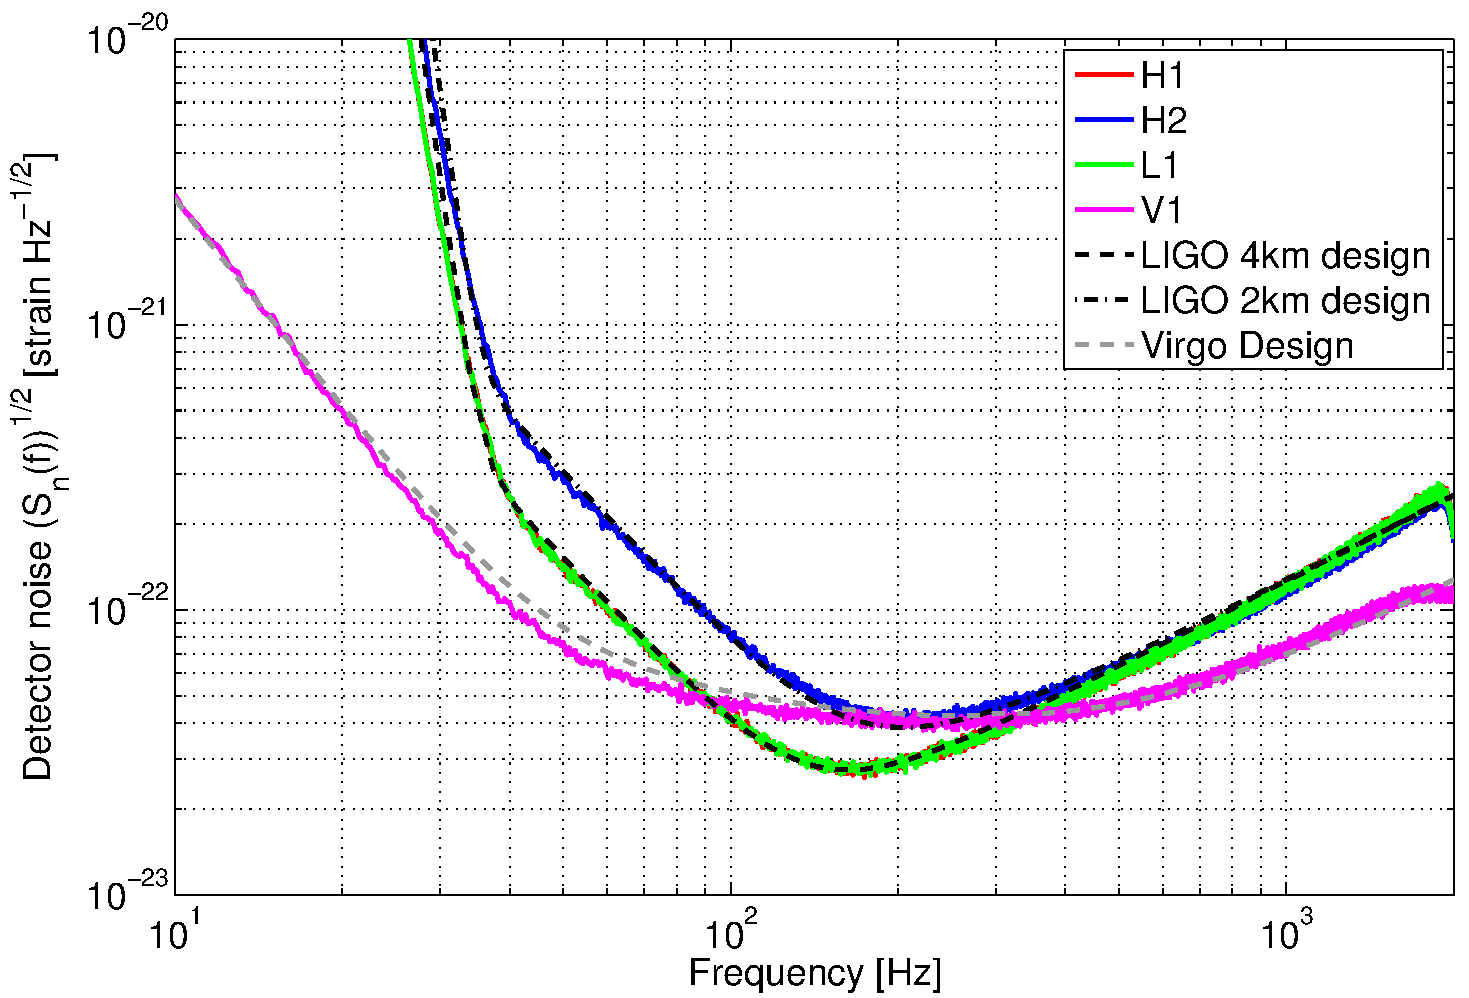
\includegraphics[width=\textwidth]{figures/ninja1/ninja_psd}
  \end{center}
  \caption[NINJA noise curves]{The NINJA data noise curves and the design spectra of the
    first generation LIGO and Virgo detectors.}
  \label{fig:ninjapsd}
\end{figure}
We see from Figure~\ref{fig:ninjapsd} that the noise power spectrum of 
the NINJA data set
closely approximates the Initial LIGO design sensitivity in the frequency
range of interest ($30$-$10^3\,$~Hz).
%The LIGO and Virgo data were
%generated using different techniques and software, and we note
There is a
slight discrepancy with the Virgo design curve at low frequencies
(between approximately $20$ and $150\,$Hz), which is an
artefact of the Virgo noise generation procedure. Narrow-band
features such as the violin and mirror modes were removed from the detector
response used to compute the NINJA data, but were included in the calculation of
the Virgo design curve~\cite{SIESTA}. The $1/f$ tails of
these narrow-band features are responsible for the small discrepancy. 

Having generated the simulated detector data, we then generated a population of
simulated signals using the numerical relativity data.  This population was
constructed to cover a broad range of masses and signal amplitudes.  We
required that the starting frequency of the dominant $\ell=m=2$ mode of the
signal was not more than $30\,$Hz, an appropriate threshold given the
sensitivity curve of the Initial LIGO and Virgo detectors.  This sets a
minimum mass at which each waveform can be injected, which is given in Table
\ref{tab:allwaveforms-SI}. The minimum possible injection mass is therefore
$36 M_{\odot}$. The maximum mass was chosen as $350 M_{\odot}$.  To
get a good sample of long injected waveforms, we systematically chose a lower
range of masses for the longer waveforms. No restrictions were placed on the
other simulation parameters, i.e., the spins, mass-ratios and eccentricities. 
We ensured that waveforms from all the participating groups were equitably
represented by generating approximately 12 signals from the waveforms supplied
by each group. The time interval between adjacent injected signals was chosen
to be a random number in the range $700\pm 100\,$~s. 

Given these constraints, we generated the parameters of the signal population.
The logarithm of the distance to the binary was drawn from a uniform
distribution ranging from $50\,$Mpc to $500\,$Mpc, and the source 
locations and orientations were drawn from an isotropic distribution of angles. 
We then computed
waveforms corresponding to this population and at the appropriate sampling
rate. We required that the optimal matched filter signal-to-noise ratio of any
injection be greater than five in at least one of the four simulated detectors.
Any waveform that did not satisfy this constraint was discarded from the
population.  Subject to this condition, the distances of injected signals varied
from $52\,$Mpc to $480\,$Mpc (median at $145\,$Mpc), the injected total mass
range was $36M_\odot \le M \le346M_\odot$ (median at $155 M_\odot$), with
individual component masses in the range $11 M_\odot \le m_i \le193M_\odot$.  

Finally, the waveforms $h(t)$ were added to the simulated detector noise
$n(t)$ to generate the NINJA data set $s(t) = n(t) + h(t)$. As described
above, care was taken to ensure that signals were coherently injected in the
data streams from the four detectors.  The software for carrying out this
procedure is freely available as part of the LSC Algorithm Library
(LAL)~\cite{lal}.

The data set used in this analysis consisted of a total of 126 signals
injected in a total of 106 contiguous segments of noise each $1024\,$ s
long, thus spanning a duration of a little over $30\,$hours.
Figure~\ref{fig:distvsmass} shows the mass, spin and distance of the waveforms
contained in the NINJA data set.
\begin{figure}
  \begin{center}
  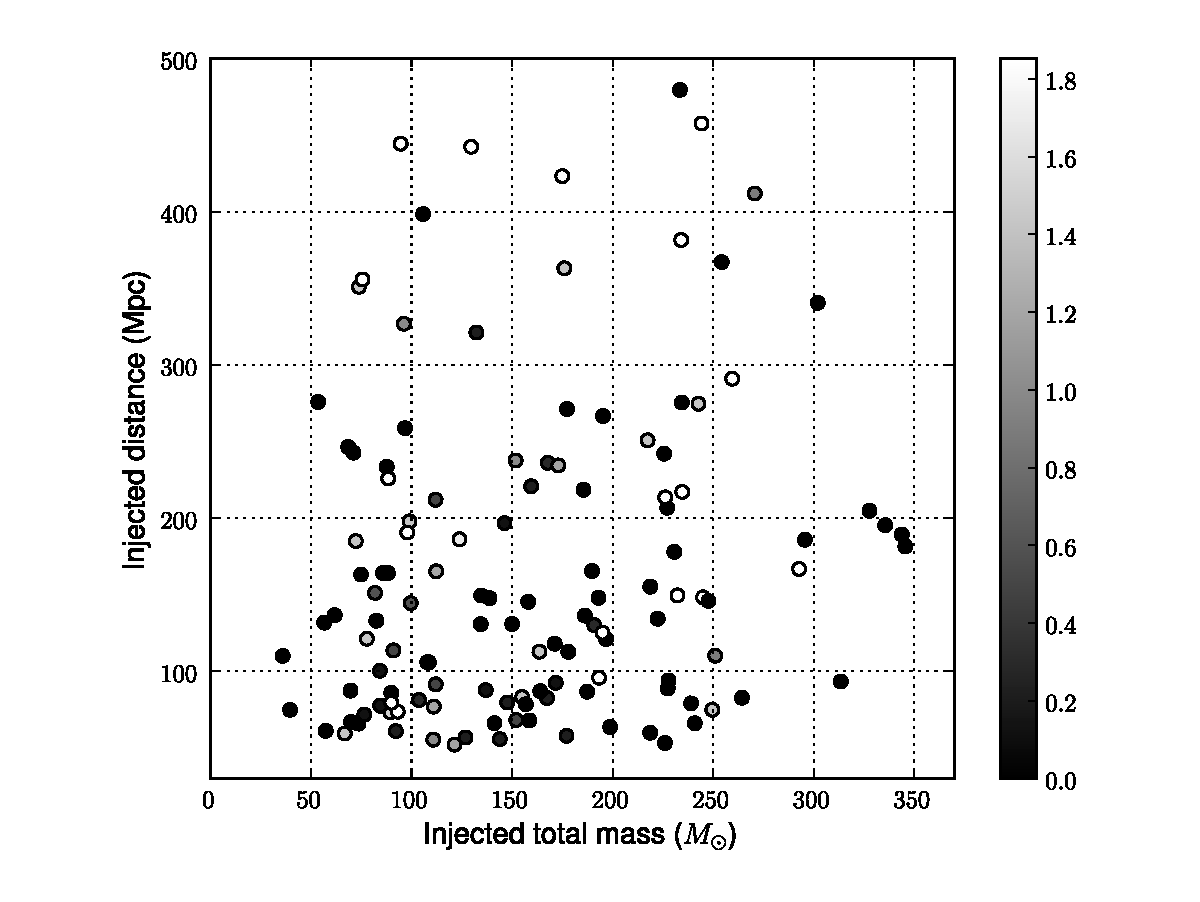
\includegraphics[width=0.9\textwidth]{figures/ninja1/DistanceVsMass_injected_withSpins}
  \end{center}
  \caption[Distribution of NINJA1 injections]{The total mass and distance of the 126 NINJA injections. The
    grey scale encodes the sum of the dimensionless spins of the black holes, 
$|\vec{S_1}/m_1^2 + \vec{S_2}/m_2^2|$.}
  \label{fig:distvsmass}
\end{figure}


\section{Data Analysis Results}
\label{sec:ninja1_da}

\subsubsection{Stationary Phase Inspiral Templates}
\label{sssec:ninja1_insp} 

% begin inspiral_templates.tex
The workhorse template of the LSC-Virgo search pipeline is based on the
stationary-phase approximation to the Fourier transform of the
non-spinning post-Newtonian inspiral~\cite{Droz:1999qx,Allen:2005fk}.
This waveform (referred to as SPA or TaylorF2) has been used in the
search for binary neutron
stars~\cite{Abbott:2003pj,Abbott:2005pe,Abbott:2007xi,Abbott:2009tt}, 
sub-solar mass black holes~\cite{Abbott:2005pf,Abbott:2007xi,Abbott:2009tt}
and stellar mass black holes~\cite{Abbott:2009tt}. The TaylorF2 waveform
is parametrised by the binary's component masses $m_1$ and $m_2$ (or
equivalently the total mass $M = m_1 + m_2$ and the symmetric mass ratio
$\eta = m_1 m_2 / M^2$) and an upper frequency cutoff $f_\mathrm{c}$.
Amplitude evolution is modelled to leading order and phase evolution is
modelled to a specified post-Newtonian order. In this section we investigate
the performance of TaylorF2-based searches on the three simulated LIGO
detectors. Results which include the simulated Virgo detector are described in
the next section.  Several analyses were performed 
which test the ability of TaylorF2 waveforms to detect numerical relativity
signals. The analyses differed in the way the TaylorF2 waveforms or the
template bank were constructed.  The results of these searches are summarised
in Table~\ref{tab:inspiral_results}, each column giving the results from a
different search with a summary of the chosen parameters.  We first describe
the parameters varied between these analyses and then present a more detailed
discussion of the results.

All TaylorF2 NINJA analyses used restricted templates (i.e.~the amplitude is
calculated to leading order), however the phase was calculated to various
different post-Newtonian orders~\cite{Blanchet:2002av}. Phases were computed to
either two~\cite{Blanchet:1996pi,Blanchet:1995ez} or three point five
post-Newtonian order~\cite{Blanchet:2001ax,PhysRevD.71.129902,Blanchet:2004ek}
since these are, respectively, the order currently used in LSC-Virgo
searches~\cite{Abbott:2009tt} and the highest order at which post-Newtonian
corrections are known. After choosing a post-Newtonian order, one chooses a
region of mass-parameter space to cover with the template bank.
Figure~\ref{f:ninjaBanks} shows the boundaries of the template banks used in
the analyses. One search used the range used by the LSC-Virgo ``low-mass''
search \cite{Abbott:2009tt} ($m_1,m_2 \ge  1 M_\odot, M \le 35 M_{\odot}$) and
all other searches used templates with total masses in the range $20 M_\odot
\le M \le 90 M_\odot$.  These boundaries were chosen since there were no
signals in the NINJA data with mass smaller than $36 M_\odot$ and there is
little, if any, inspiral power in the sensitive band of the NINJA data for
signals with $M \gtrsim 100 M_\odot$.  The standard LSC-Virgo template bank
generation code~\cite{Babak:2006ty} restricts template generation to signals
with $\eta \le 0.25$, since it is not possible to invert $M$ and $\eta$ to
obtain real-valued component masses for $\eta > 0.25$. All but one of the
searches enforced this constraint, with the $0.03 \le \eta \le 0.25$ for the
low-mass CBC search and $0.1 \le \eta \le 0.25$ for the other
``physical-$\eta$'' searches. It is, however, possible to generate TaylorF2
waveforms with ``unphysical'' values of $\eta > 0.25$.  In two separate studies
using Goddard and Pretorius waveforms~\cite{Pan:2007nw}, and Caltech-Cornell
waveforms~\cite{Boyle:2009dg} it was observed that match between numerical
signals and TaylorF2 templates could be increased by relaxing the condition
$\eta \le 0.25$. One NINJA contribution uses a template bank with $0.1 \le \eta
\le 1.0$ to explore this.

Finally, it is necessary to specify a cutoff frequency at which to terminate the
TaylorF2 waveform. In the LSC-Virgo analyses, this is chosen to be the
innermost stable circular orbit (ISCO) frequency for a test mass in a
Schwarzschild spacetime 
%
\begin{equation}
\label{f_ISCO}
f_\mathrm{ISCO} = \frac{c^3}{6\sqrt{6}\pi GM}.
\end{equation}
%
This cutoff was chosen as the point beyond which the TaylorF2 waveforms
diverge significantly from the true evolution of the
binary~\cite{Blanchet:2002av}.  More recently, comparisons with numerical
relativity waveforms have shown that extending the waveforms up to higher
frequencies improves the sensitivity of TaylorF2 templates to higher mass
signals~\cite{Pan:2007nw,Boyle:2009dg}. The NINJA TaylorF2 analyses use
templates terminated at the ISCO frequency and two additional cut-off
frequencies: the effective ringdown (ERD) frequency and a weighted
ringdown ending (WRD) frequency. The ERD frequency was obtained by comparing
post-Newtonian models to the Pretorius and Goddard
waveforms~\cite{Pan:2007nw}. The ERD almost coincides with the fundamental
quasi-normal mode frequency of the black hole formed by the merger of an
equal-mass non-spinning black-hole binary. The weighted ringdown ending (WRD)
frequency lies between ISCO and ERD, and was obtained by comparing
TaylorF2 waveforms to the Caltech-Cornell numerical
signals~\cite{Boyle:2009dg}.

\begin{table}
\begin{tabular}{| l || c | c | c | c | c | c | c |}
\hline
\bf{Analysis} \T \B & $(1)$ & $(2)$ & $(3)$ & $(4)$ & $(5)$ & $(6)$ \\ \hline
\bf{Freq. Cutoff} \T \B & ISCO & ISCO & ERD & ERD &  WRD & WRD  \\ 
\hline
\bf{PN Order} & 2 PN & 2 PN & 2 PN & 3.5 PN &  3.5 PN& 3.5 PN  \\
\hline
%\parbox{2.8cm}{
%\bf{Component\\ Mass $M_{\odot}$}} & 1--34 & 10--60 & 10--60 & 10--60 & 10--60 & 10--60 \\ 
%\hline
\bf{Total Mass $M_{\odot}$} \T \B & 2--35 & 20--90 & 20--90 & 20--90 & 20--90 & 20--90  \\ 
\hline
\bf{$\eta$ range} \T \B & 0.03--0.25 & 0.10--0.25 & 0.10--0.25 & 0.10--0.25 & 0.10--0.25 & 0.10--1  \\ 
\hline
\parbox{2.3cm}{
\bf{Found Single\\ (H1, H2, L1)}}\TT \BB  & 69, 66, 75 & 72, 43, 66 & 83, 51, 81 & 91, 56, 87 & 90, 55, 88 & 90, 56, 88 \\ 
\hline
\parbox{2.3cm}{
\bf{Found \\Coincidence }} \TT \BB & 49 & 59 & 79 & 82 &  82 & 84 \\ 
\hline
\parbox{2.5cm}{
\bf{Found Second\\Coincidence}} \TT \BB & 48 & 59 & 77 & 81 &  81 & 81 \\ 
\hline 
\end{tabular}
\caption{{\bf Results of inspiral searches using TaylorF2 templates.}  There were 126
injections performed into the data.  The table above shows the number of
injections which were recovered from the three simulated LIGO detectors (H1, H2 and L1) using various different waveform families,
termination frequencies $f_\mathrm{ISCO}$, $f_\mathrm{ERD}$ and $f_\mathrm{WRD}$ 
(as described in the text), and post-Newtonian orders.} 
\label {tab:inspiral_results}
\end{table}


\begin{figure}
  \begin{center}
  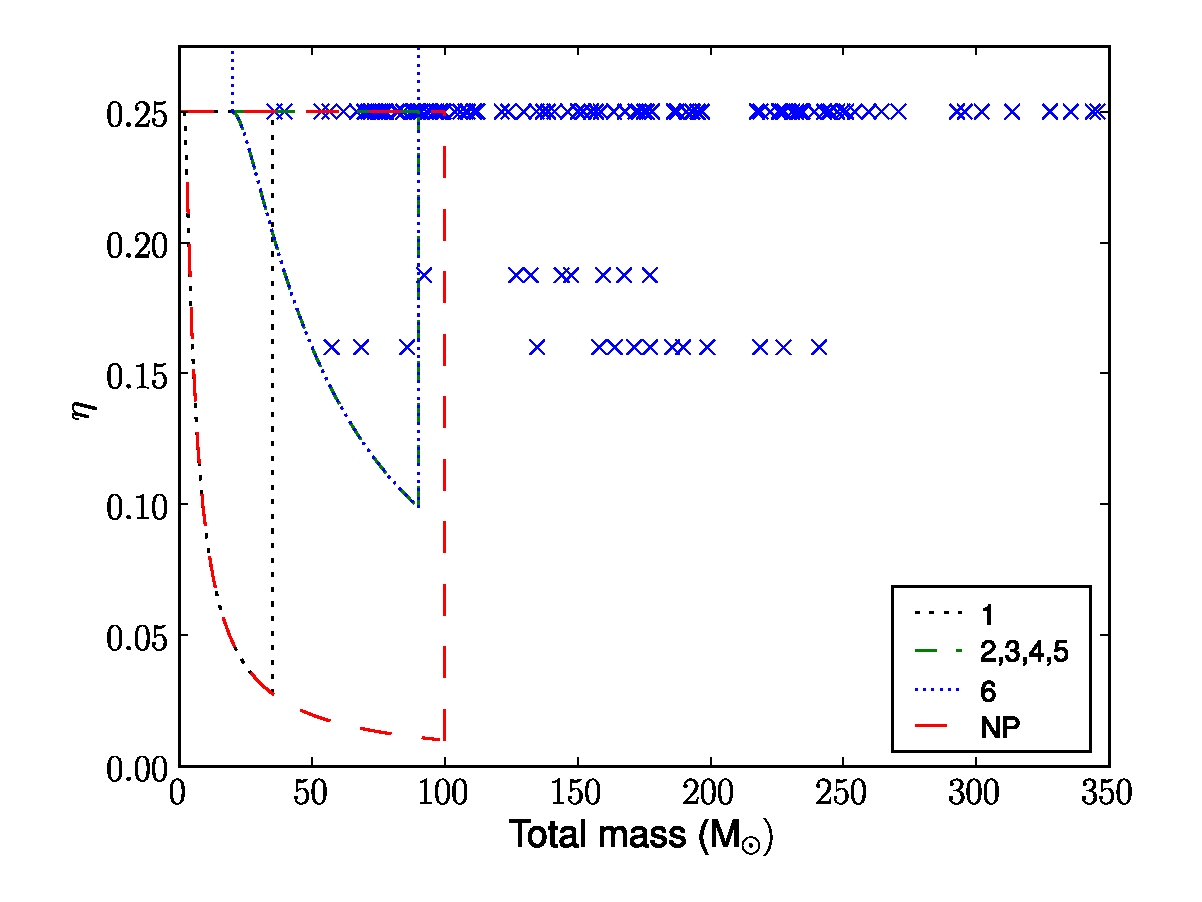
\includegraphics[width=0.8\textwidth]{figures/ninja1/ninja_banks}
  \end{center}
  \caption[Boundaries of template banks in NINJA1 inspiral searches]{
Boundaries of the template banks used in inspiral searches as a
  function of total mass $M$ and symmetric mass ratio $\eta$. The crosses show
  the location of the injections in the NINJA data set. The numbers in the
  legend correspond to entries in table~\ref{tab:inspiral_results}. Bank 6
  extends in a rectangle up to $\eta = 1.00$, as indicated by the arrows. NP
  is the bank used in the Neyman-Pearson analysis described in 
  Section~\ref{sssec:neyman}.}
  \label{f:ninjaBanks}
\end{figure}

The results of these searches are reported in
Table~\ref{tab:inspiral_results}.  The principal result is the number
of injected signals detected by the search.  For simplicity, we define
a detected signal as one for which there is a candidate
gravitational-wave signal observed within $50$~ms of the coalescence
time of the injection, determined by the maximum gravitational-wave
strain of the injected signal.  We do not impose any additional
threshold on the measured SNR or effective SNR of the candidate.  For
a single detector, this will lead to a small number of falsely
identified injections, but for coincidence results the false alarm
rate is so low that we can be confident that the triggers are
associated with the injection. We now describe these results in the
order that they appear in Table~\ref{tab:inspiral_results}.

Search~$(1)$ used second order post-Newtonian templates terminated at
$f_\mathrm{ISCO}$ with a maximum mass of $M \le 35 M_{\odot}$.
Despite the fact that no NINJA injections had a mass within the range
of this search, a significant number of signals were still recovered
in coincidence both before and after signal consistency tests.
Although the templates are not a particularly good match to the
injected signals, they are still similar enough to produce triggers at
the time of the injections.  Search~$(2)$ changed the boundary of the
template bank to $20 M_\odot \le M \le 90 M_{\odot}$, but left all
other parameters unchanged.  The number of detected signals increases
significantly as more signals now lie within the mass range searched. 

Search~$(3)$ extended the upper cutoff frequency of the waveforms to
$f_\mathrm{ERD}$. The number of signals detected increased from 59 to
77, as expected since these waveforms can detect some of the power
contained in the late inspiral or early merger part of the
signal~\cite{Pan:2007nw,Boyle:2009dg}. Search~$(4)$ extends the
post-Newtonian order to 3.5~PN, slightly increasing the number of
detected signals to 81.  With the limited number of simulations
performed in this first NINJA analysis, it is difficult to draw a
strong conclusion, although there does seem to be evidence that the
higher post-Newtonian order waveforms perform better, consistent with
previous comparisons of post-Newtonian and numerical relativity
waveforms
\cite{Pan:2007nw,Baker:2006ha,Hannam:2007ik,Boyle:2008ge,Boyle:2009dg}.
Search~$(5)$ uses an upper-frequency cutoff of $f_\mathrm{WRD}$ for
the templates. The number of injections found in coincidence for this
search is the same as the search using $3.5$ order templates with a
cutoff of $f_\mathrm{ERD}$, although there are slight differences in
the number of found injections at the single detector level.

Search~$(6)$ extends the template bank of search~$(5)$ to unphysical
values of the symmetric mass ratio. Extending the bank to $\eta\le 1$
increases the number of templates in the bank by a factor of $\sim 2$.
The original and modified template banks are shown in
Figure~\ref{f:templateBanks}. With the extended template bank the
number of injections found in coincidence remains the same as
search~$(5)$ after signal-based vetoes are applied.  However, many of
the injections are recovered at a higher SNR, particular the low-mass
signals, as shown in Figure~\ref{f:templateBanks}.  Some injections
show a reduction in SNR; more work is needed to understand this
effect.

\begin{figure}
  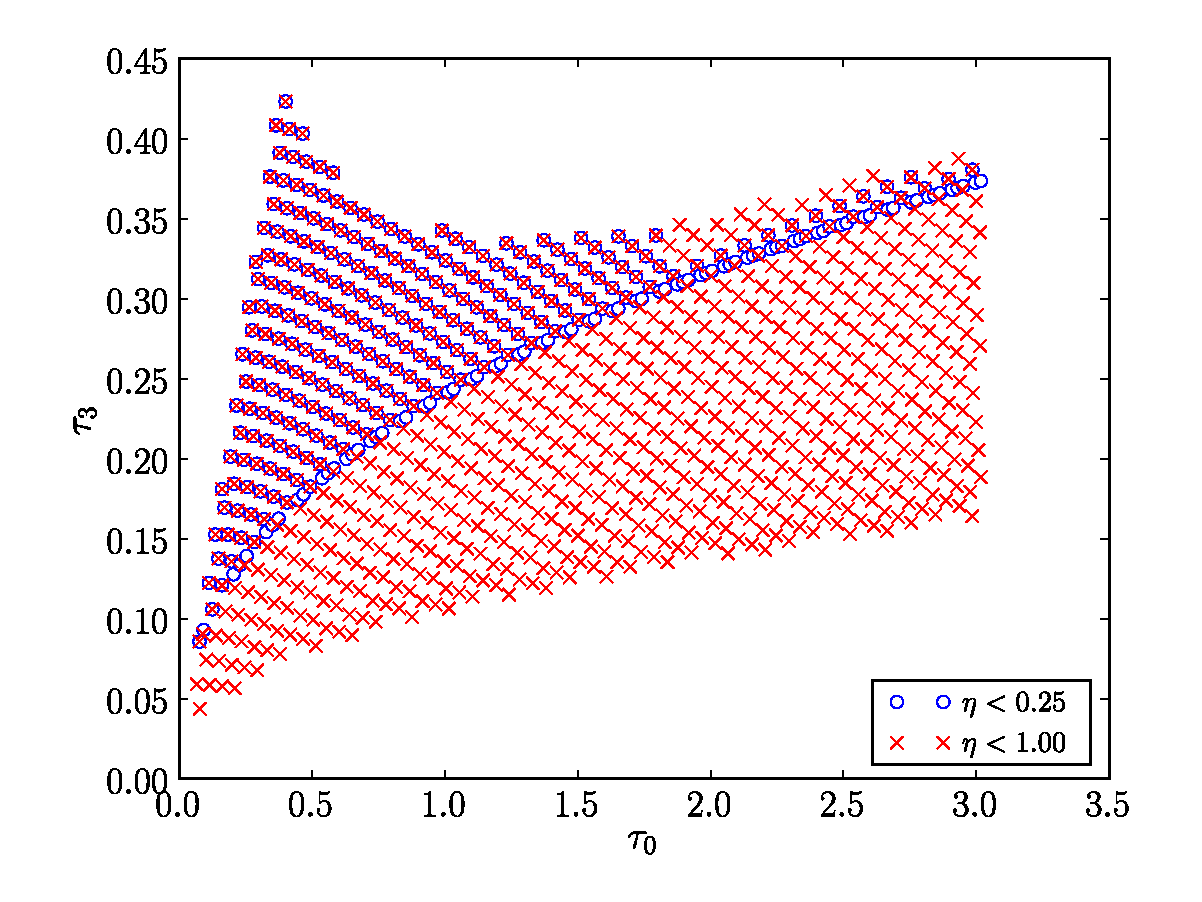
\includegraphics[width=0.50\textwidth]{figures/ninja1/BankBoth}
  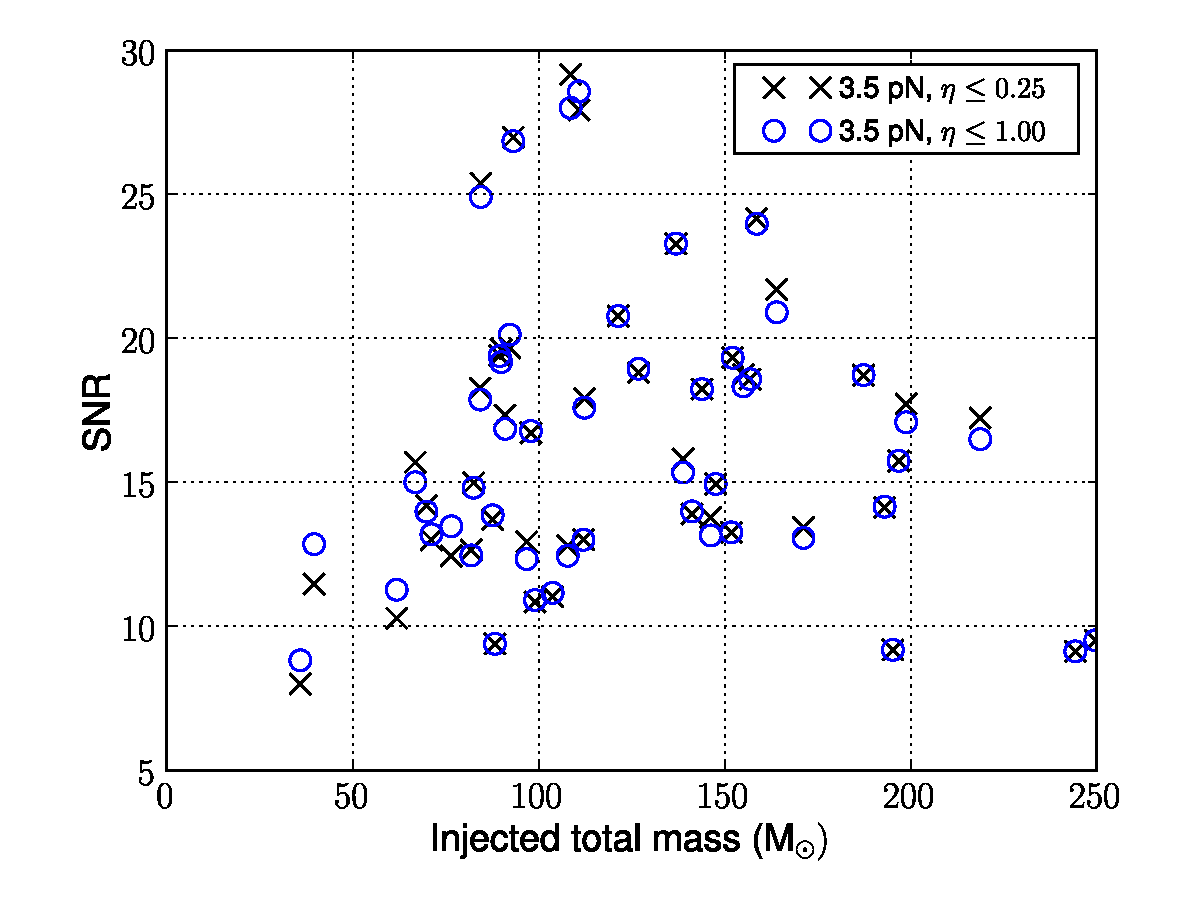
\includegraphics[width=0.50\textwidth]{figures/ninja1/HanfordSNR}
  \caption[NINJA1 results from the extended template bank]{
  {\bf Left:} The template bank generated by the LSC-Virgo
  search pipeline (circles) and the bank obtained by extending to
  $\eta \leq 1.00$ (crosses). In this figure the bank is parametrised
  by $\tau_0$ and $\tau_3$ which are related to the binary masses by
  $\tau_0 = 5M/(256\eta v_0^8)$ and $\tau_3 = \pi M/(8\eta v_0^5)$,
  where $v_0 = (\pi M f_0)^{1/3}$ is a fiducial velocity parameter
  corresponding to a fiducial frequency $f_0 = 40.0 Hz$.
  {\bf Right:} The
  signal-to-noise (SNR) ratio at which NINJA injections were recovered using
  the $\eta \le 0.25$ bank (squares) and the $\eta \le 1$ extended bank
  (circles) in the Hanford detectors, given by $\rho =
  (\rho_\mathrm{H1}^2 + \rho_\mathrm{H2}^2)^{1/2}$. The SNR of the signal
  recovered using the extended bank shows with significant ($> 10\%$) 
  increases over the standard bank for certain injections.}
  \label{f:templateBanks}
\end{figure}

Finally, we note that the majority of signals passed the $\chi^2$
signal-based veto with the thresholds used in the LSC-Virgo pipeline.  The
last two lines of Table~\ref{tab:inspiral_results} show the number of
recovered signals before and after these signal-based vetoes are
performed. The post-Newtonian templates and numerical relativity signals are
similar enough that virtually all of the injected signals survive the signal
based vetoes. 

To illustrate the results of these analyses in more detail, 
Figure~\ref{fig:3_5pn_found_missed} shows which signals were detected and which were
missed by the 3.5 order post-Newtonian TaylorF2 templates terminated at
$f_\mathrm{ERD}$, as a function of injected
total mass and effective distance of the binary (a measure of the
amplitude of the signal in the detector), defined by~\cite{Allen:2005fk}
\begin{equation}
D_\mathrm{eff} = d \left/ \sqrt{F_+^2 (1 + \cos^2 \iota)^2/4 + F_\times^2 \cos^2 \iota}\right.,
\label{eq:effdist}
\end{equation}
where $d$ is the luminosity distance of the binary.

One signal, with total mass of $110 M_{\odot}$ and effective distance $\sim
200$ Mpc, was missed while others with similar parameters were found.  This
signal was one of the Princeton waveforms (labelled \verb|PU-e0.5| in
Figure \ref{fig:NR-Reh22}) for which the maximum amplitude occurs at the start
of the waveform rather than at coalescence\footnote{That the maximum 
occurs at the start of the waveform is in part an ``artifact'' of the 
double-time integration from the Newman-Penrose scalar $\psi_4$ to the 
metric perturbation $h$, and in part a coordinate artifact.
The two integration constants were chosen to remove a 
constant and linear-in-time piece for $h$, however, there is still 
a non-negligible quadratic component; we {\em suspect} this is purely gauge, 
though lacking a better understanding of this it was not removed from the 
waveform.}, rendering our simple coincidence
test invalid.  The injection finding algorithm compares the peak time to the
trigger time and, even though triggers are found at the time of the simulation,
there are no triggers within the $50$~ms window used to locate detected
signals.

\begin{figure}
\begin{center}
  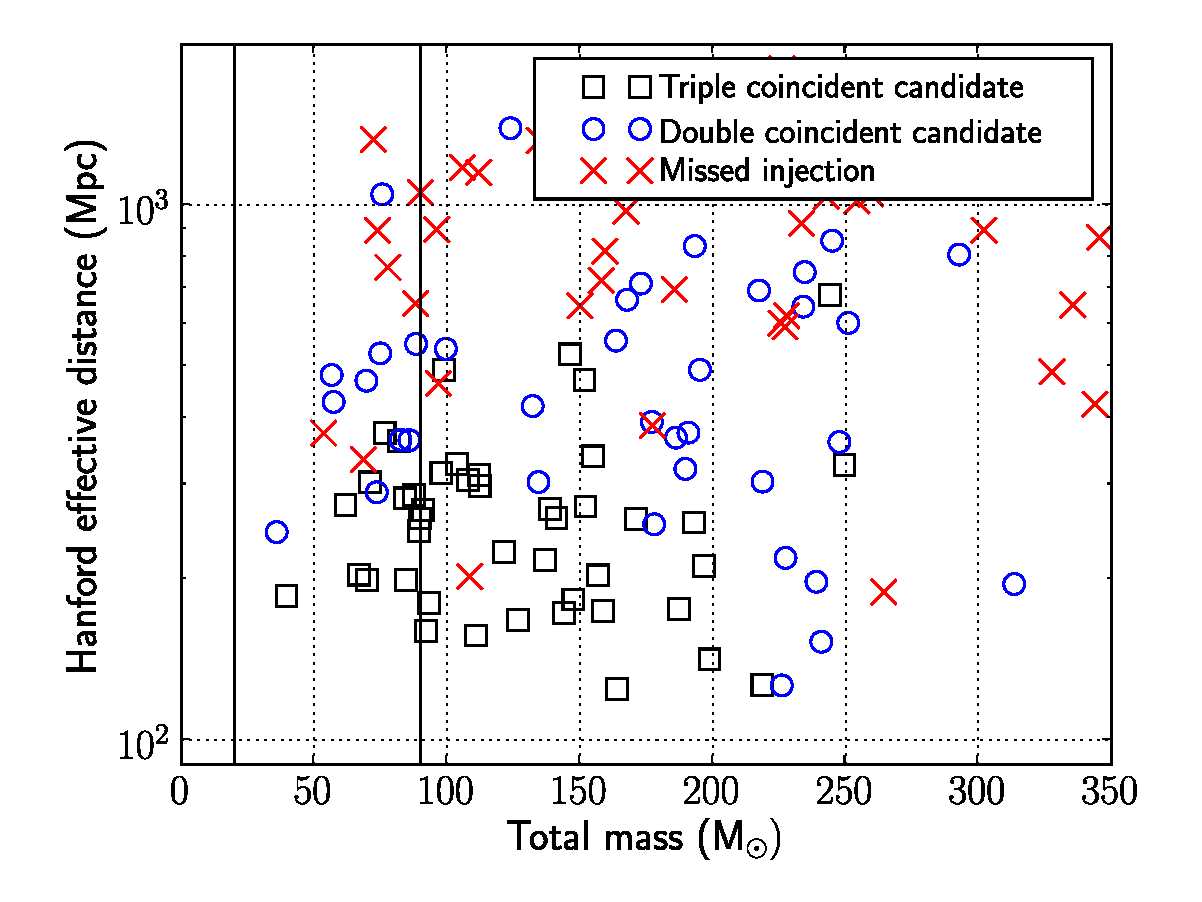
\includegraphics[width=0.49\textwidth]{figures/ninja1/spa_erd_3_5pn_found_missed_mchirp}
  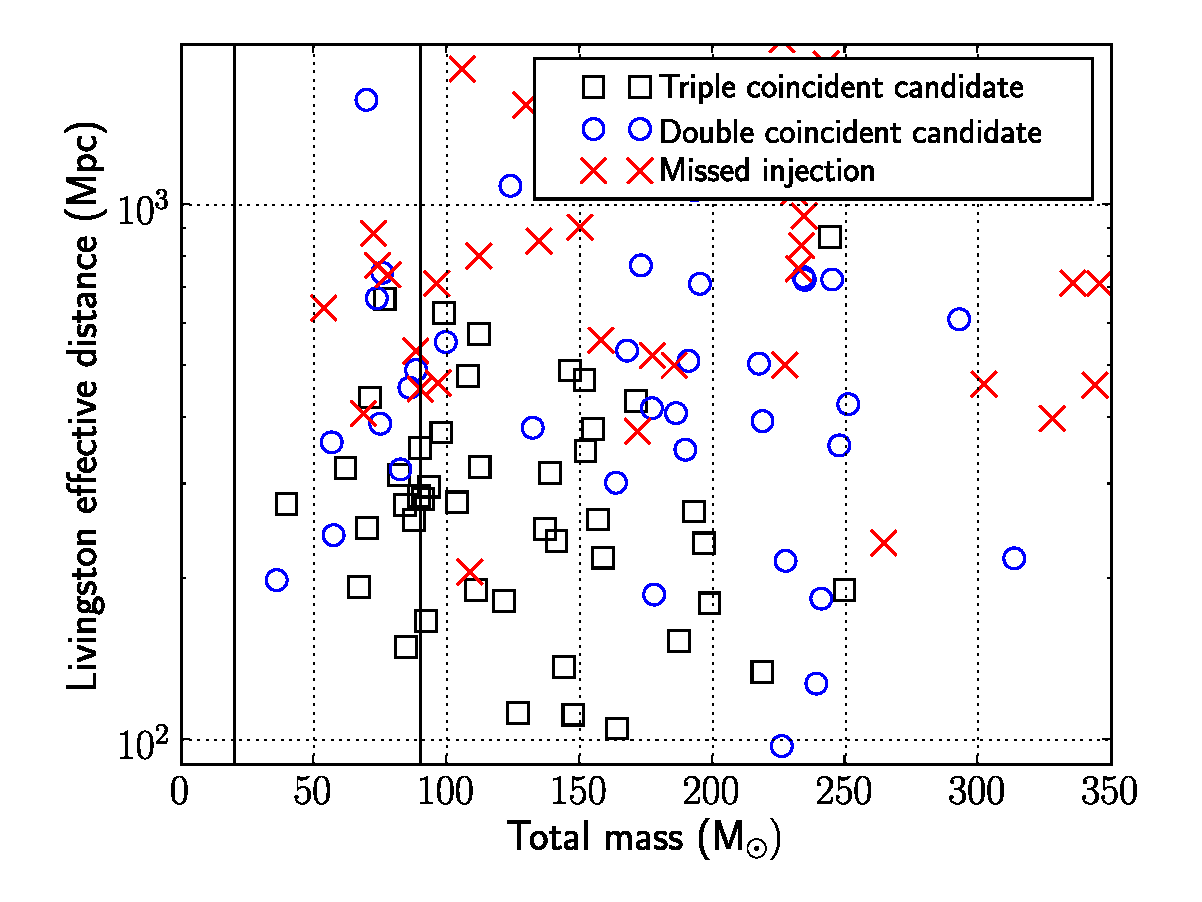
\includegraphics[width=0.49\textwidth]{figures/ninja1/spa_erd_3_5pn_found_missed_mchirp_l}
\end{center}
\caption[NINJA1 injections found/missed by an inspiral search with
$f_c=$ ERD.]{
\label{fig:3_5pn_found_missed}
Found and missed injections using TaylorF2 templates
terminated at ERD, plotted as a function of the injected effective
distance in Hanford (left) and Livingston (right) and the total mass
of the injection. Since the LIGO Observatories are not exactly
aligned, the effective distance of a signal can differ, depending on
the sky location of the signal.  The vertical bars mark the limits of
the template bank used in the search.  For the lower masses, we see
that the majority of the closer injections are found in coincidence in
all three of the detectors.  There is then a band of injections which
are found only in two detectors -- H1 and L1 and not the less
sensitive H2 detector.  For higher masses, the results are less
meaningful as the template bank was only taken to a total mass of $90
M_{\odot}$.}
\end{figure}

Figure~\ref{fig:3_5pn_params} shows the accuracy with which the total mass and
coalescence time of the binary are recovered when using the 3.5 post-Newtonian
order Taylor F2 templates. The total mass fraction difference is computed as
$(M_\mathrm{injected} - M_\mathrm{detected})/ M_\mathrm{injected}$. For lower
mass signals, the end time is recovered reasonably accurately, with accuracy
decreasing for the high mass systems. The total mass recovery is poor for the
majority of signals, with good parameter estimation for only a few of the
lowest mass simulations.

\begin{figure}
    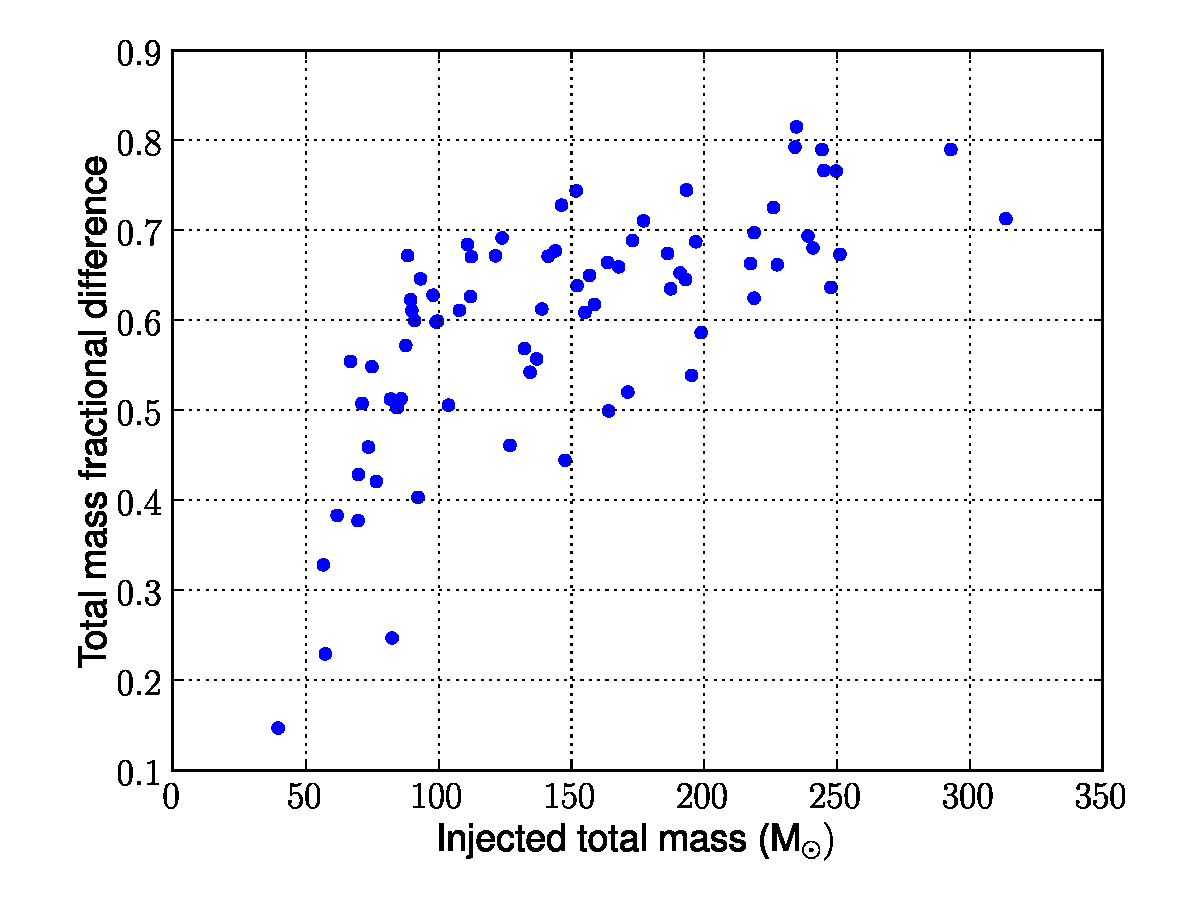
\includegraphics[width=0.50\textwidth]{figures/ninja1/spa_erd_3_5pn_mass_estimate}
    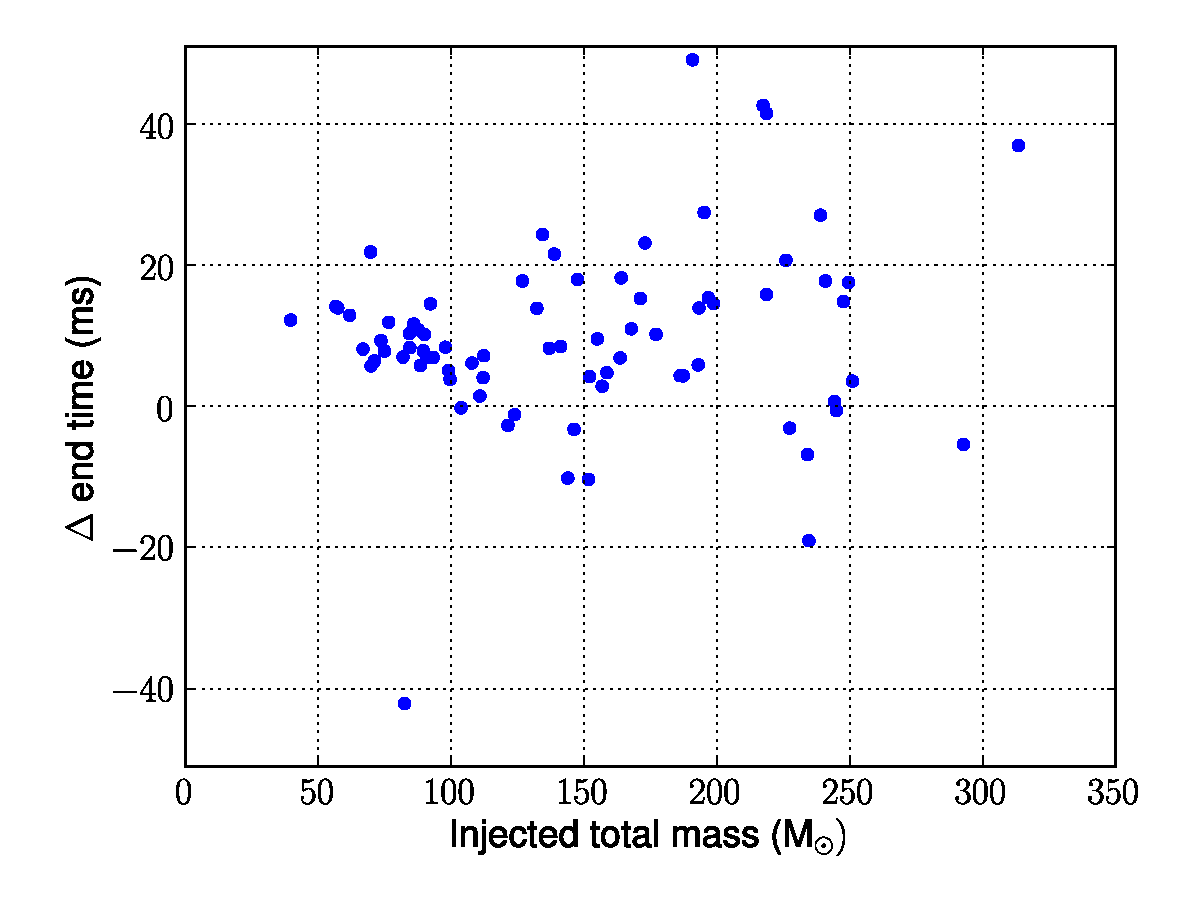
\includegraphics[width=0.50\textwidth]{figures/ninja1/spa_erd_3_5pn_time_estimate_vs_mt}
\caption[Parameter accuracy using TaylorF2 templates terminated at ERD]{
\label{fig:3_5pn_params}
Parameter accuracy using TaylorF2 templates terminated at
ERD.\textbf{Left:} Accuracy with which the total mass is recovered. The
template bank covers the region $20 M_\odot \le M \le 90 M_\odot$, hence
the mass of injections with $M > 90 M_\odot$ are always underestimated.
Even within the region covered by the bank, the TaylorF2 templates
systematically underestimate the mass of the injected signals and the total
mass is recovered accurately only for a few injections.  The vast majority of
recoverd signals have an error of $40\%$ or greater. \textbf{Right:} Accuracy
of determining the coalescence time of the injections.  The end time is not
recovered accurately, the timing error can become as large as $50
\mathrm{ms}$, the limits of the injection window.  }
\end{figure}

% end inspiral_templates.tex







\Chapter{Waveform Analysis for the Second NINJA project}
\label{ch:ninja2}
The NINJA-1 project was a huge success in bringing the numerical
relativity and gravitational-wave astronomy communities together.  The
project also resulted in several intriguing qualitative results.
However, it only began the process of testing detection and parameter
estimation pipelines against realistic signals.  The follow-up
project, NINJA-2, is ongoing as of the time of writing.  NINJA-2 aims
to remove some of the shortcomings of NINJA-1 and allow quantitative
studies of the behaviors of pipelines in varying regions of signal
parameter space.  Specifically, NINJA-2 addresses issues with both the
waveform submissions and the noise used to construct the data sets.

This chapter describes the contributed waveforms, the studies that
have been done to verify them, and the construction of the first round
of data sets.  The next chapter will present preliminary results from
running the CBC pipelines on the longest and most carefully
constructed of these data sets.

\section{Contributed waveforms}

NINJA-1 had an open policy towards waveforms submission in order to
encourage wide participation.  This meant there were no requirements
on either waveform quality or length.  The lack of quality
requirements allowed for the possibility of unphysical features in the
waveforms.  There were also no requirements to perform the kind of
convergence testing reported in section~\ref{sec:PNNRHybridWaveform},
although such validation is typically done by numerical
relativistists.  The loose requirements limited the conclusions that
could be drawn, for example it makes it difficult to say whether an
injection was missed due to the parameters of the signal or an
unintended feature of the waveform.

The lack of length requirement limited the available mass range to $M
< 36 \msun$ for reasons that can be seen in
figure~\ref{fig:StildesAndInitialPSD}.   Had the waveform in that plot
not had a post-Newtonian component, the NR component to the right of
the triangles would have had to be placed below 40 Hz in order to
prevent turning on in-band.  This mass range limited the tests that
could be done, for example it entirely excludes the standard CBC
low-mass pipeline.

To address these issues NINJA-2 specifies the following minimal
requirements~\cite{ninja2-wiki}.  The raw numerical simulation should
include at least five orbits of usable data before merger (i.e., not
counting bursts of junk radiation or other significant noise).  Given
the computation cost of extending the NR waveforms, we instead require
stitching to a post-Newtonian inspiral approximant, which should be
performed at a GW frequency of $M\omega ≤ 0.075$, where $M\omega$ is
the frequency of the $(l = 2, m = \pm 2)$ harmonic. The full waveform
should be long enough to be entirely within the sensitivity bands of
LIGO and Virgo down to $10 \msun$ with a lower cutoff frequency of 10
Hz, which corresponds to a starting GW frequency of $M\omega = 0.003$.
The numerical-waveform (before any hybridization) amplitude should be
accurate to within 5\%, and the phase (as a function of GW frequency)
should have an accumulated uncertainty over the entire inspiral,
merger and ringdown, of no more than 0.5 radian. The PN approximants
used for hybridization should ideally use the highest PN orders
available, both in phase and amplitude.  

These minimal accuracy requirements are motivated by the results of
the Samurai project~\cite{Hannam:2009hh}, and studies performed in
preparation for the NR-AR collaboration project~\cite{ninja-wiki}.
The question of how many NR cycles are needed in order to produce a
robust waveform is an area of current research. \Note{cite Ilana}.

The NINJA-2 project encourages although does not require the addition
of higher-order modes.  We chose to restrict attention to non-spinning
waveforms and waveforms with spins aligned or anti-aligned with the
orbital angular momentum.  There are sufficient open questions
regarding these restricted cases to make this analysis interesting,
without adding the additional complications on both the NR and data
analysis sides associated with precession. 

A total of 60 waveforms from 8 groups were contributed, these are
summarized in tables ~\ref{tab:ninja2_bam}, \ref{tab:ninja2_fau},
\ref{tab:ninja2_gatech}, \ref{tab:ninja2_lean},
\ref{tab:ninja2_llama}, \ref{tab:ninja2_rit}, \ref{tab:ninja2_spec},
\ref{tab:ninja2_uiuc} and a map of the parameter values is shown in
figure~\ref{f:ninja2_param_map}.

\begin{table}
\begin{center}
\begin{tabular}{|l|r|r|r|l|c|}
\hline
Run & $q$ & Spin1${}_z$ & Spin2${}_z$ & pN Approx. & Refs \\
\hline
BAM\_D10spp85\_80.T4.hyb.n2 & 1 & 0.85 & 0.85 & TaylorT4 & \cite{Hannam:2007wf,Brugmann:2008zz} \\
BAM\_D10spp85\_80.T1.hyb.n2 & 1 & 0.85 & 0.85 & TaylorT1 & \cite{Hannam:2007wf,Brugmann:2008zz} \\
BAM\_D125smm50Nep\_80.T1.hyb.n2 & 1 & -0.50 & -0.50 & TaylorT1 & \cite{Hannam:2007wf,Brugmann:2008zz} \\
BAM\_D125smm50Nep\_80.T4.hyb.n2 & 1 & -0.50 & -0.50 & TaylorT4 & \cite{Hannam:2007wf,Brugmann:2008zz} \\
BAM\_D13smm75Nep\_96.T4.hyb.n2 & 1 & -0.75 & -0.75 & TaylorT4 & \cite{Hannam:2007wf,Brugmann:2008zz} \\
BAM\_D13smm75Nep\_96.T1.hyb.n2 & 1 & -0.75 & -0.75 & TaylorT1 & \cite{Hannam:2007wf,Brugmann:2008zz} \\
BAM\_D13smm85Nep\_88.T4.hyb.n2 & 1 & -0.85 & -0.85 & TaylorT4 & \cite{Hannam:2007wf,Brugmann:2008zz} \\
BAM\_D13smm85Nep\_88.T1.hyb.n2 & 1 & -0.85 & -0.85 & TaylorT1 & \cite{Hannam:2007wf,Brugmann:2008zz} \\
BAM\_D11spp50\_96.T4.hyb.n2 & 1 & 0.50 & 0.50 & TaylorT4 & \cite{Hannam:2007wf,Brugmann:2008zz} \\
BAM\_D11spp50\_96.T1.hyb.n2 & 1 & 0.50 & 0.50 & TaylorT1 & \cite{Hannam:2007wf,Brugmann:2008zz} \\
BAM\_D10spp75\_80.T1.hyb.n2 & 1 & 0.75 & 0.75 & TaylorT1 & \cite{Hannam:2007wf,Brugmann:2008zz} \\
BAM\_D10spp75\_80.T4.hyb.n2 & 1 & 0.75 & 0.75 & TaylorT4 & \cite{Hannam:2007wf,Brugmann:2008zz} \\
BAM\_D12smm25Nep\_80.T4.hyb.n2 & 1 & -0.25 & -0.25 & TaylorT4 & \cite{Hannam:2007wf,Brugmann:2008zz} \\
BAM\_D12smm25Nep\_80.T1.hyb.n2 & 1 & -0.25 & -0.25 & TaylorT1 & \cite{Hannam:2007wf,Brugmann:2008zz} \\
BAM\_EP\_um4\_D10-n96.T4.hyb.n2 & 4 & 0.00 & 0.00 & TaylorT4 & \cite{Hannam:2007wf,Brugmann:2008zz} \\
BAM\_EP\_um4\_D10-n96.T1.hyb.n2 & 4 & 0.00 & 0.00 & TaylorT1 & \cite{Hannam:2007wf,Brugmann:2008zz} \\
BAM\_um3\_88.T4.hyb.n2 & 3 & 0.00 & 0.00 & TaylorT4 & \cite{Hannam:2007wf,Brugmann:2008zz} \\
BAM\_um3\_88.T1.hyb.n2 & 3 & 0.00 & 0.00 & TaylorT1 & \cite{Hannam:2007wf,Brugmann:2008zz} \\
BAM\_um2\_88.T1.hyb.n2 & 2 & 0.00 & 0.00 & TaylorT1 & \cite{Hannam:2007wf,Brugmann:2008zz} \\
BAM\_um2\_88.T4.hyb.n2 & 2 & 0.00 & 0.00 & TaylorT4 & \cite{Hannam:2007wf,Brugmann:2008zz} \\
BAM\_R6\_PN\_80.T1.hyb.n2 & 1 & 0.00 & 0.00 & TaylorT1 & \cite{Hannam:2007wf,Brugmann:2008zz} \\
BAM\_R6\_PN\_80.T4.hyb.n2 & 1 & 0.00 & 0.00 & TaylorT4 & \cite{Hannam:2007wf,Brugmann:2008zz} \\
BAM\_D12spp25\_96.T4.hyb.n2 & 1 & 0.25 & 0.25 & TaylorT4 & \cite{Hannam:2007wf,Brugmann:2008zz} \\
BAM\_D12spp25\_96.T1.hyb.n2 & 1 & 0.25 & 0.25 & TaylorT1 & \cite{Hannam:2007wf,Brugmann:2008zz} \\
BAM\_q2a0a025\_T\_96\_344.T1.hyb.n2.bbh & 2 & 0.25 & 0.00 & {} & \cite{,Brugmann:2008zz} \\
BAM\_q2a0a025\_T\_96\_344.T4.hyb.n2.bbh & 2 & 0.25 & 0.00 & {} & \cite{,Brugmann:2008zz} \\
\hline
\end{tabular}
\end{center}
\caption[BAM submissions to NINJA-2]{
\label{tab:ninja2_bam}
BAM submissions to NINJA-2}
\end{table}

\begin{table}
\begin{center}
\begin{tabular}{|l|r|r|r|l|c|}
\hline
Run & $q$ & Spin1${}_z$ & Spin2${}_z$ & pN Approx. & Refs \\
\hline
BAM\_hybrid\_om0.025etmq3S0.4- & 3 & 0.40 & 0.60 & TaylorT4 & \cite{none,???} \\
0\_0\_S0.6\_0\_0\_72 &  &  &  &  &  \\
\hline
\end{tabular}
\end{center}
\caption[FAU submissions to NINJA-2]{
\label{tab:ninja2_fau}
FAU submissions to NINJA-2}
\end{table}

\begin{table}
\begin{center}
\begin{tabular}{|l|r|r|r|l|c|}
\hline
Run & $q$ & Spin1${}_z$ & Spin2${}_z$ & pN Approx. & Refs \\
\hline
MayaKranc\_D12\_a0.00\_m129\_nj & 1 & 0.00 & 0.00 & TaylorT4 & \cite{,} \\
MayaKranc\_D10\_a0.90\_m129\_nj & 1 & 0.90 & 0.90 & TaylorT4 & \cite{,} \\
MayaKranc\_D10\_a0.20\_m77\_nj & 1 & 0.20 & 0.20 & TaylorT4 & \cite{,} \\
MayaKranc\_D10\_a0.60\_m77\_nj & 1 & 0.60 & 0.60 & TaylorT4 & \cite{,} \\
MayaKranc\_D12\_a0.60\_m103\_nj & 1 & 0.60 & 0.60 & TaylorT4 & \cite{,} \\
MayaKranc\_Sp02py0935th90\_gr & 1 & 0.80 & 0.00 & TaylorT4 & \cite{,} \\
MayaKranc\_D12\_a0.80\_m103\_nj & 1 & 0.80 & 0.80 & TaylorT4 & \cite{,} \\
MayaKranc\_D12\_a0.00\_q2\_m90\_nj & 2 & 0.00 & 0.00 & TaylorT4 & \cite{,} \\
MayaKranc\_D11\_a0.20\_q2\_m90\_nj & 2 & 0.02 & 0.09 & TaylorT4 & \cite{,} \\
MayaKranc\_D10\_a0.40\_m90\_nj & 1 & 0.40 & 0.40 & TaylorT4 & \cite{,} \\
MayaKranc\_D10\_a0.80\_m90\_nj & 1 & 0.80 & 0.80 & TaylorT4 & \cite{,} \\
MayaKranc\_D12\_a0.40\_m103\_nj & 1 & 0.40 & 0.40 & TaylorT4 & \cite{,} \\
MayaKranc\_D12\_a0.20\_m103\_nj & 1 & 0.20 & 0.20 & TaylorT4 & \cite{,} \\
\hline
\end{tabular}
\end{center}
\caption[GATech submissions to NINJA-2]{
\label{tab:ninja2_gatech}
GATech submissions to NINJA-2}
\end{table}

\begin{table}
\begin{center}
\begin{tabular}{|l|r|r|r|l|c|}
\hline
Run & $q$ & Spin1${}_z$ & Spin2${}_z$ & pN Approx. & Refs \\
\hline
dq4 & 4 & 0.00 & 0.00 & TaylorT1 & \cite{,Sperhake:2006cy} \\
\hline
\end{tabular}
\end{center}
\caption[LEAN submissions to NINJA-2]{
\label{tab:ninja2_lean}
LEAN submissions to NINJA-2}
\end{table}

\begin{table}
\begin{center}
\begin{tabular}{|l|r|r|r|l|c|}
\hline
Run & $q$ & Spin1${}_z$ & Spin2${}_z$ & pN Approx. & Refs \\
\hline
Llama\_d550-h64-Hybrid & 1 & 0.00 & 0.00 & 3.5pNTaylorF2 & \cite{Reisswig:2009rx,Reisswig:2009rx} \\
Llama\_d4d4-q1--D10-h64-r250.T4.hybrid & 1 & -0.40 & -0.40 & TaylorT4 & \cite{Pollney:2010hs,Pollney:2009yz,} \\
Llama\_d4d4-q1--D10-h64-r250.T1.hybrid & 1 & -0.40 & -0.40 & TaylorT1 & \cite{Pollney:2010hs,Pollney:2009yz,} \\
Llama\_u4u4-q1--D8-h64-r250.T1.hybrid & 1 & 0.40 & 0.40 & TaylorT1 & \cite{Pollney:2010hs,Pollney:2009yz,} \\
Llama\_u4u4-q1--D8-h64-r250.T4.hybrid & 1 & 0.40 & 0.40 & TaylorT4 & \cite{Pollney:2010hs,Pollney:2009yz,} \\
Llama\_d5q2-h016-Hybrid & 2 & 0.00 & 0.00 & 3.5pNTaylorF2 & \cite{,Reisswig:2009rx} \\
Llama\_u2u2-q1--D8-h64-r250.T1.hybrid & 1 & 0.20 & 0.20 & TaylorT1 & \cite{Pollney:2010hs,Pollney:2009yz,} \\
Llama\_u2u2-q1--D8-h64-r250.T4.hybrid & 1 & 0.20 & 0.20 & TaylorT4 & \cite{Pollney:2010hs,Pollney:2009yz,} \\
Llama\_d2d2-q1--D10-h64-r250.T1.hybrid & 1 & -0.20 & -0.20 & TaylorT1 & \cite{Pollney:2010hs,Pollney:2009yz,} \\
Llama\_d2d2-q1--D10-h64-r250.T4.hybrid & 1 & -0.20 & -0.20 & TaylorT4 & \cite{Pollney:2010hs,Pollney:2009yz,} \\
\hline
\end{tabular}
\end{center}
\caption[Llama submissions to NINJA-2]{
\label{tab:ninja2_llama}
Llama submissions to NINJA-2}
\end{table}

\begin{table}
\begin{center}
\begin{tabular}{|l|r|r|r|l|c|}
\hline
Run & $q$ & Spin1${}_z$ & Spin2${}_z$ & pN Approx. & Refs \\
\hline
LazEV\_D8.4\_10to1\_nj\_hybrid & 10 & 0.00 & 0.00 & TaylorT4 & \cite{Campanelli:2005dd} \\
\hline
\end{tabular}
\end{center}
\caption[RIT submissions to NINJA-2]{
\label{tab:ninja2_rit}
RIT submissions to NINJA-2}
\end{table}

\begin{table}
\begin{center}
\begin{tabular}{|l|r|r|r|l|c|}
\hline
Run & $q$ & Spin1${}_z$ & Spin2${}_z$ & pN Approx. & Refs \\
\hline
SpEC\_q6s0 & 6 & 0.00 & 0.00 & TaylorT1 & \cite{SpECWebsite} \\
SpEC\_q4s0 & 4 & 0.00 & 0.00 & TaylorT2 & \cite{SpECWebsite} \\
SpEC\_EqualMassAntiAlignedSpins & 1 & -0.44 & -0.44 & NA & \cite{chu-2009,SpECWebsite} \\
SpEC\_q1s-0.95 & 1 & -0.95 & -0.95 & TaylorT1 & \cite{SpECWebsite} \\
SpEC\_q2s0 & 2 & 0.00 & 0.00 & TaylorT2 & \cite{SpECWebsite} \\
SpEC\_EqualMassAlignedSpins & 1 & 0.44 & 0.44 & NA & \cite{chu-2009,SpECWebsite} \\
SpEC\_q3s0 & 3 & 0.00 & 0.00 & TaylorT2 & \cite{SpECWebsite} \\
SpEC\_EqualMassNonspinning & 1 & 0.00 & 0.00 & TaylorT4 & \cite{Scheel:2008rj,SpECWebsite} \\
\hline
\end{tabular}
\end{center}
\caption[SpEC submissions to NINJA-2]{
\label{tab:ninja2_spec}
SpEC submissions to NINJA-2}
\end{table}

\begin{table}
\begin{center}
\begin{tabular}{|l|r|r|r|l|c|}
\hline
Run & $q$ & Spin1${}_z$ & Spin2${}_z$ & pN Approx. & Refs \\
\hline
UIUC\_spin\_-0.25\_om0.0528\_22-HYBRID & 1 & -0.25 & -0.25 & NA & \cite{none} \\
UIUC\_spin\_0.85\_om0.0536\_22-HYBRID & 1 & 0.85 & 0.85 & NA & \cite{none} \\
\hline
\end{tabular}
\end{center}
\caption[UIUC submissions to NINJA-2]{
\label{tab:ninja2_uiuc}
UIUC submissions to NINJA-2}
\end{table}


\begin{figure}
  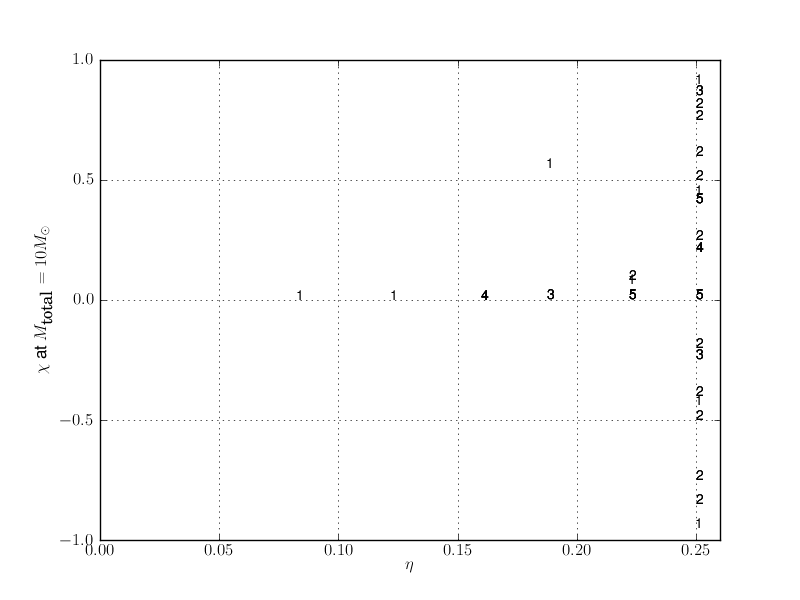
\includegraphics[width=\linewidth]{figures/ninja2/ninja2_cat.png}
  \caption[Parameters of the NINJA-2 submissions]{
  \label{f:ninja2_param_map}
Parameters of the NINJA-2 hybrid waveform submissions showing the
symmetric mass ratio $\eta=m_1 m_2 /(m_1+m_2)^2$ and dimensionless
spin parameter $\chi=(S_1/m_1 + S_2/m_2)/(m_1+m_2)$ after scaling the
waveforms to a total mass of 10 $\msun$.  The numbers indicate how
many distinct waveforms with the specified parameters were submitted.}
\end{figure}%

\section{Verifying the hybrid waveforms}

Each NR group verified that their waveforms met the minimum NINJA-2
requirements before submission.  Once submitted, a series of checks
were performed in order to validate the waveforms against each other.

In the first stage the post-Newtonian expressions and codes were
compared against each other and the literature.  This required several
iterations, but resulted in a set of codes in various languages that
produce waveforms that all agree in both phase and amplitude. 

\subsection{Time-domain and frequency-domain checks}

In the second stage the complete hybrid waveforms were examined.
We first plotted the last 40 cycles of each waveform -- enough to
include the full NR portion, the hybridization region, and some of the
pN portion -- and looked for any anomalies such as those present in
some of the NINJA-1 waveforms in figure~\ref{fig:NR-Reh22}.  A few such
features were indeed visible, spotting them in this way allowed them
to be corrected.  One example is shown in figure (\Note{show the dq4
waveform before and after, note this was due to a problem integrating
psi4, and discuss this stage a little in the NR section of chapter
3}).

The amplitude of the Fourier transform of the complete waveforms were
also plotted.  This analysis also revealed unphysical features, 
primarily due to hybridization.  An example is shown in
figure~\ref{f:ninja2_freq_hybrids}, which shows a visible ``kink'' in
the waveform at the hybridization frequency, which vanishes after the
waveform was reconstructed.

\begin{figure}
  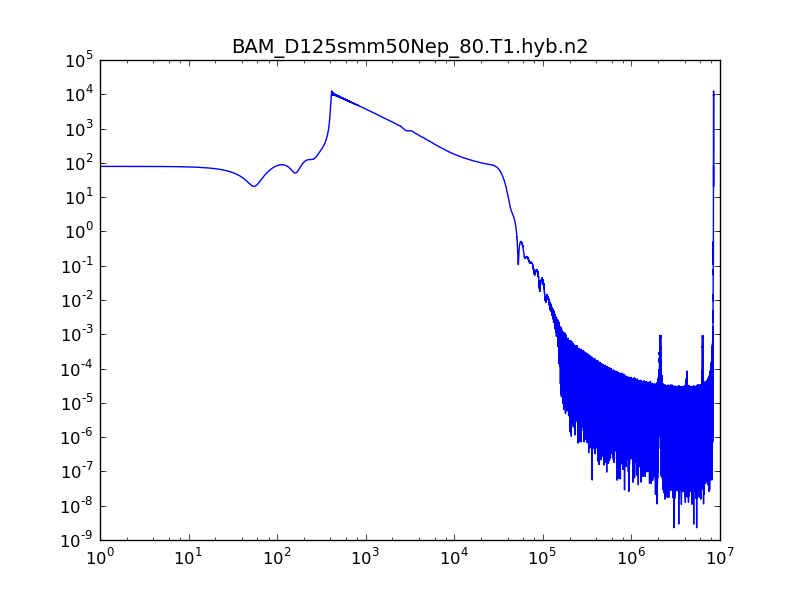
\includegraphics[width=0.5\linewidth]{figures/ninja2/bam_d125smm50nep_80_t1_hyb_n2_amp.png}
  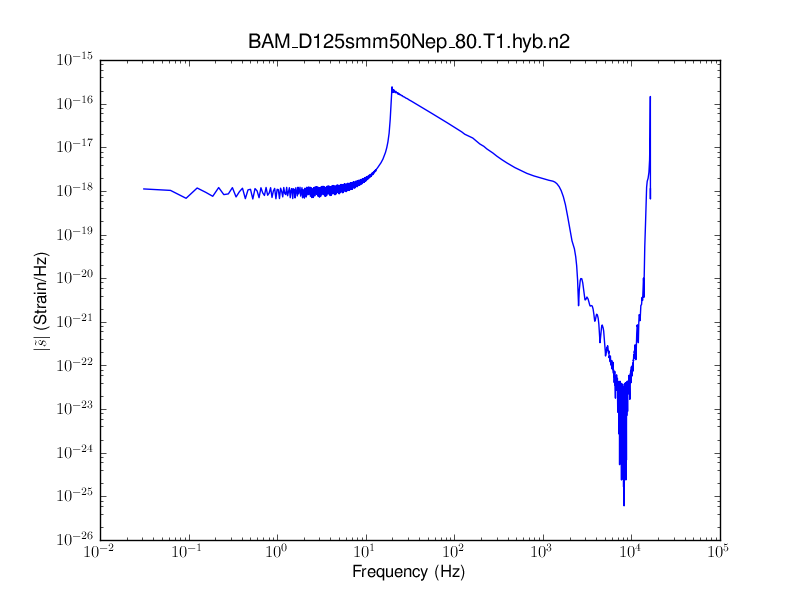
\includegraphics[width=0.5\linewidth]{figures/ninja2/bam_d125smm50nep_80_t1_hyb_n2_amp_v2.png}
  \caption[Frequency-domain hybrid NINJA-2 waveforms]{
  \label{f:ninja2_freq_hybrids}
Fourier amplitude of the (2,2) mode of a sample NINJA-2 hybrid
waveform from the BAM/AEI group.  The waveform has been scaled to 10
$\msun$ and placed 1 Mpc from the detector to give it physical units.
\Note{I need to dig up the old version of the waveform and remake it
with the new code} The waveform on the left is the version
initially submitted, note there is a visible ``kink'' in the waveform
at the hybridization frequency.  The waveform on the right has been
re-hybridized and there is no longer a visible kink.  This feature did
not show up in the time domain view of the waveform.}
\end{figure}%


\subsection{Overlap comparisons}

In tis check the waveforms were compared against each other using
standard data-analysis techniques, in particular the overlap defined
in section~\ref{sec:search_matchfilter}. 

\begin{figure}
  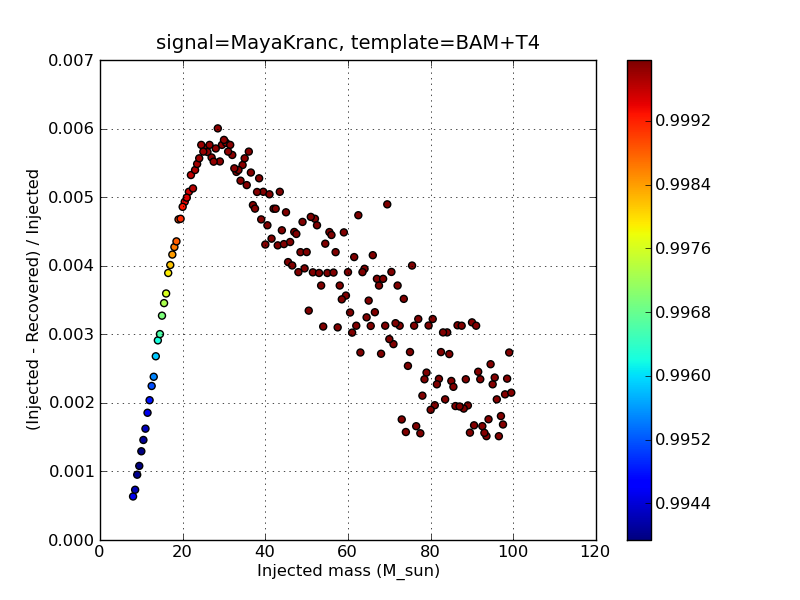
\includegraphics[width=0.5\linewidth]{figures/ninja2/maya_bamt4_max_over_m}
  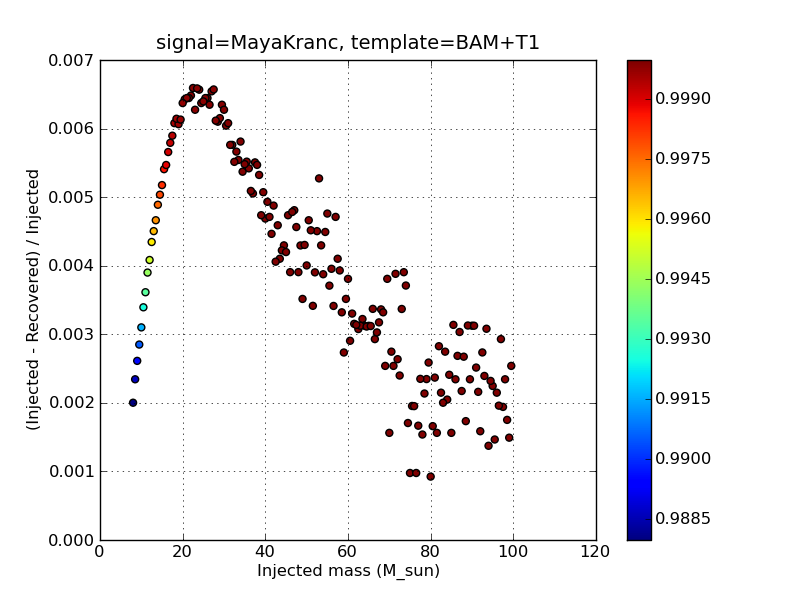
\includegraphics[width=0.5\linewidth]{figures/ninja2/maya_bamt1_max_over_m}
  \caption[Overlaps between NINJA-2 submissions maximized over mass]{
  \label{f:ninja2_max_over_mass_bam}
Overlaps between the equal-mass, non-spinning MayaKranc waveform taken
as the signal, and the equal-mass, non-spinning BAM waveform
hybridized with TaylorT4 (left) and TaylorT1 (right) taken as
templates.  Maximization is done over mass, as well as time and phase.
Note the lower overall overlaps and mass bias at the low-mass end,
where the two pN waveforms dominate the overlap.}
\end{figure}%


\section{Construction of the NINJA-2 data set}

\begin{figure}
  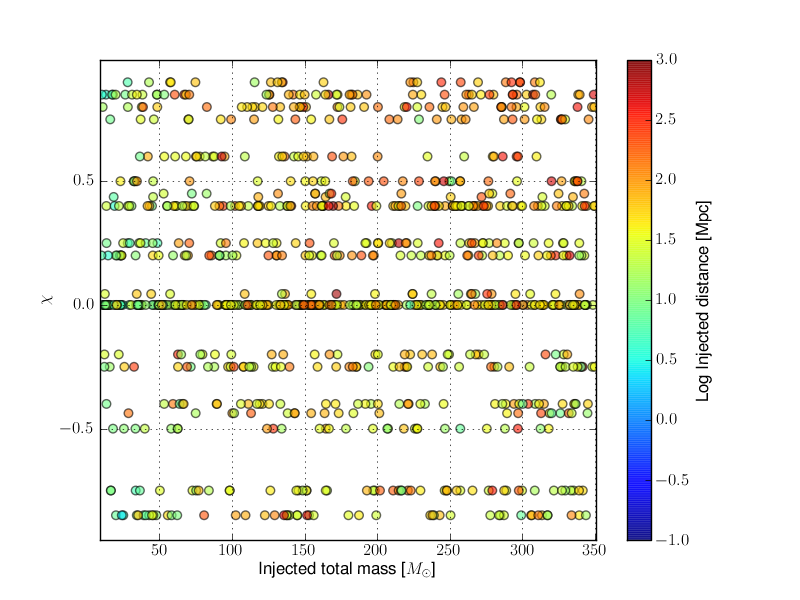
\includegraphics[width=\linewidth]{figures/ninja2/ninja2_dataset.png}
  \caption[Parameters of the NINJA-2 two-month data set]{
  \label{f:ninja2_dataset}
Distribution of mass, spin and distance parameters in the two-month,
Gaussian-noise data set.
}
\end{figure}%



% TODO:
% make tables of submissions
% plot of paramater space in eta, chi scaled to 10 M
% plot of injection set (use chi instead of sum of magnitudes)
% text
% results
% explain move to 16384 (plot showing aliasing)



\Chapter{Preliminary CBC Results from the Second NINJA project}
\label{ch:ninja2_results}
In the previous chapter we discussed the hybrid pN/NR waveforms
contributed to the NINJA-2 project, along with the studies performed
to validate them.  We now turn to the data analysis portion of
NINJA-2, including the data sets and some preliminary results.

\section{Construction of the NINJA-2 data set}

In broad terms the plans for the NINJA-2 data sets follow those for
NINJA-1 (ch.~\ref{ch:ninja1}).  Simulated Gaussian noise was generated
to model the initial LIGO and Virgo noise curves, the spectra are
identical to those in figure~\ref{f:ninjapsd}.  Injection parameters,
including choice of waveform, were then selected randomly.  The
injections were then added to the Gaussian noise and distributed to
data analysis groups.  However, several key changes were made in the
details of this process in order to correct shortcomings in NINJA-1.  

The NINJA-2 data was sampled at 16384 Hz rather than the 4096 Hz used
by NINJA-1.  This was done because investigations showed that there is
power above 4096 Hz in the waveforms, which would get aliased down to 
lower frequencies if the sample rate is too low.  This problem is
illustrated in figure~\ref{f:ninja2_aliasing}.

\begin{figure}
  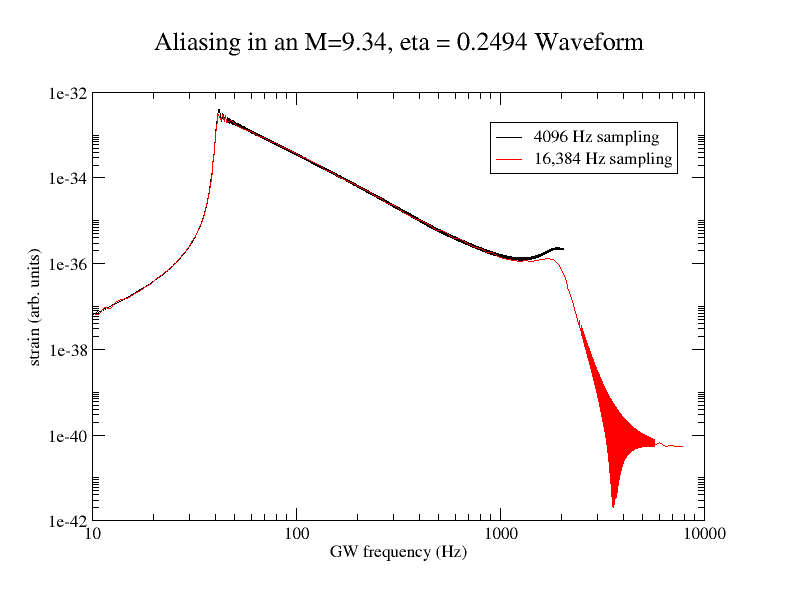
\includegraphics[width=\linewidth]{figures/ninja2_results/ninja2_aliasing}
  \caption[Aliasing of waveform power]{
  \label{f:ninja2_aliasing}
Frequency-domain amplitudes of a NINJA-2 waveform at different
sampling rates.  At a sample rate of 4096 Hz the late portion of the
waveform are distorted due to aliasing of power to lower frequencies.
}
\end{figure}%

Note that this is a different issue from the one that motivated
performing the waveform overlaps at 32768 Hz, discussed in
section~\ref{ssec:ninja2_overlap_comparisons}.  The issue there was
that undersampling could miss the maximum of the overlap function.
The issue here is that undersampling can distort the end of the
waveform.

NINJA-1 consisted of only 127 injections in one day of data, which
severely limited the ability to draw statistical conclusions on the
behavior of the pipelines.  To correct this in NINJA-2 we extended the
duration to eight weeks.  The density of injections was varied over
this span:  weeks 1-3 had one injection on average every 2000 seconds,
week 4-6 had one injection on average every 14,400 seconds, and the
final two weeks had one injection every on average every 216,000
seconds.  The intent is that data analysts can tune and test their
pipelines on the dense weeks, and then optionally perform a
self-blinded test on the final two weeks.

In NINJA-1 the SNR was not chosen a priori but was determined by the
other parameters.  For NINJA-2 we draw the network SNR ($\sqrt{\sum_i
\rho_i^2}$ where $i$ ranges over the IFOs) from a distribution and
then scale the distance of the injection in order to achieve that SNR.
For the first three weeks the distribution is linear from 6 to 130 in
order to allow pipelines to test and tune out to large SNRs on the
densest set of injections.  For the remaining weeks the distribution
falls as the reciprocal of the network SNR (uniform in
$\log(\mathrm{SNR})$) in order to better model the expected
astrophysical distribution.

The mass and waveform selection were also done slightly differently in
NINJA-2.  For each injection a mass was first selected uniformly over
the specified range; for the full 2-month run this range is from
$10-350 \msun$.  Then waveforms were selected at random until one was
found that could be injected at the chosen mass such that the waveform
turns on below 35 Hz.  In practice this condition never caused any
waveform to be rejected, as all submitted waveforms were long enough
to be injected down to the lowest mass in the range.  The mass ratio
and spins are intrinsic to the waveforms, so choosing a submission
amounts to a choice of these parameters as well. 

As in NINJA-1 the sky location and inclination were chosen uniformly
at random.

Four NINJA-2 data sets were released:

\begin{itemize}
\item A test set consisting of one week of data was released on May 13, 2010.  This
included three separate sets spanning different mass regions;
low-mass ($10\msun - 40 \msun$), high-mass ($35 \msun - 100 \msun$)
and a burst/ringdown set ($80 \msun - 350 \msun$).  This purpose of
this run was to shake out bugs in the injection code and waveforms,
several of which were found.

\item A second test set consisting of one week of data for each of the
three mass bins was released on May 31, 2010.  This was meant to test
the fixes implemented after the first test set, and to do more
careful sanity checks.  Some results from this run are discussed in
section~\ref{sec:ninja2_test_week}.

\item Based on positive results from analyses of the second test week,
full two-month data sets for all three mass bins were released on June
9, 2010.  Unfortunately shortly after release a remaining major bug in
the injection software was discovered.  Data is stored in frame files
spanning 4096 seconds.  When an injection crossed frame boundaries
this bug would cause the portion contained in the earlier frame to be
omitted.  This happened in enough cases to invalidate the entire data
set.

\item There was then a lengthy pause, in large part due to the
LIGO-Virgo ``blind injection challenge'' (see
section~\ref{sec:applications_dog}).  However, it was during this time
that the validations discussed in the previous chapter were performed.
It was also in this gap that studies discovered the need to move to
16Hz sampling.   This quadrupled the size of the data and made the
release of 3 separate mass ranges unfeasable.  Therefore a single set
spanning two months and containing injections from $10 \msun - 350
\msun$ was released on June 13, 2011.  Analysis on this set has begun
and some preliminary results will be discussed in
section~\ref{sec:ninjna2_two_months}
\end{itemize}


There are two motivations for constructing and distributing the data
sets as NINJA-1 and NINJA-2 thus far have done.  The first is to
ensure that every group is looking at the same set of injections so
that results can be compared.  The second is due to the terms of the
NINJA agreement, which restricted distribution of the raw NR
waveforms.  However, distribution of such static sets limits the
ability of individual groups to tune their pipelines in optimal ways,
and conceptually distributing a set of parameters would be sufficient
to compare results across pipelines.  In addition the size of the data
sets makes distribution slow and complex.  The NR groups within NINJA
have therefore relaxed the conditions on their use of their waveforms.
Consequently, subsequent NINJA-2 data sets will be distributed as sets
of parameters, and data analysis groups will use the available code to
either create data sets locally, or perform the injections ``on the
fly'' as the analysis is performed.  This will also allow groups to do
special-purpose tuning runs or analyses by injecting specialized 
sets of injections into noise.  The results of these studies may be
published as short-author papers subject to the conditions of the
NINJA agreement.

So far we have focused on simulated Gaussian noise, however as we will
see in the next chapter this is not a good model for the real
detectors.  Real detector data contains many ``glitches'' caused by
both environmental factors and transient behavior of the instruments.
These glitches produce a population of background triggers.  In
testing pipelines a critical issue is the ability to distinguish such
background triggers from signals.  If NINJA is to be able to to make
definitive statements about the behavior of pipelines it is therefore
imperative to use real detector noise.  A memorandum of understanding
has been signed between the NINJA collaboration and the LIGO and Virgo
collaborations allowing the use of real noise from the 5th LIGO and
first Virgo science runs.  There are a number of technical issues to
be resolved before this can be done, however the key results from
NINJA-2 will come from on-the-fly injections into real noise.

\section{CBC Results from the second one-week data set}
\label{sec:ninja2_test_week}

As noted above, two one-week data sets were produced for testing the
injection code and performing sanity checks on the results.  Here we
present the results of running the standard low-mass CBC pipeline on
the low-mass data set from the second of these runs.  As this was
largely a testing and debugging exercise no effort was made to draw
conclusions about the pipelines.  In particular, no runs were
performed with a bank extended to unphysical $\eta$ or the other
pipeline modifications suggested by the studies in
chapter~\ref{ch:comparison} and tested in NINJA-1.

The injection parameters were chosen as described above, the selected
masses, spins and distances are shown in
figure~\ref{f:ninja2_test_dataset}.

\begin{figure}
  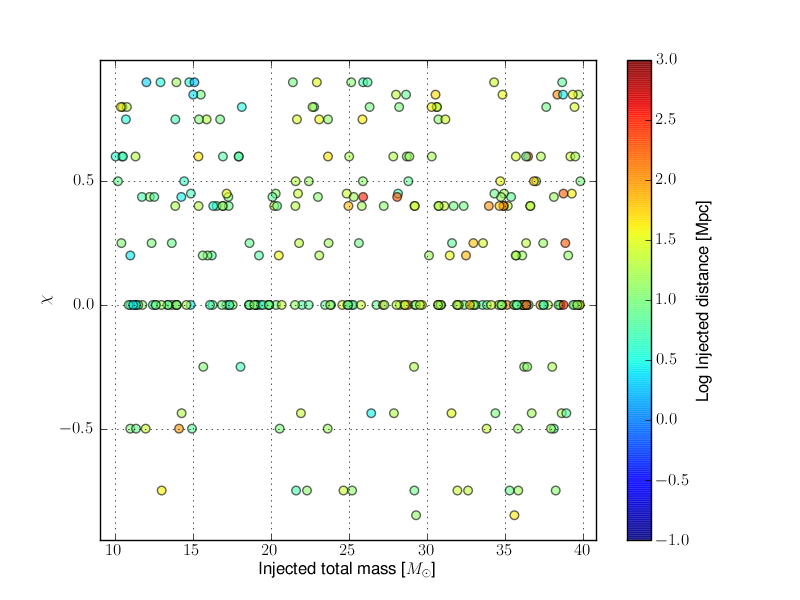
\includegraphics[width=\linewidth]{figures/ninja2_results/ninja2_test_dataset.png}
  \caption[Parameters of the NINJA-2 test one-week data set]{
  \label{f:ninja2_test_dataset}
Distribution of mass, spin and distance parameters in the one-week,
Gaussian-noise test data set.
}
\end{figure}%


The S6 version of the standard CBC low-mass pipeline was run over this
data set.  This version of the pipeline uses Taylor F2
stationary-phase templates taken to 3.5 pN order in phase evolution.
The first result of interest is the found/missed plots at the first
stage, before the $\chisq$ test or coincidence between detectors has
been applied.  The result for the H1 detector is shown in
figure~\ref{f:first_stage}.  This can give some indication of how well
the waveforms and the bank capture the signals.  However, it can also
be misleading.  The pipeline considers an injection to be ``found'' if
there is a trigger within 100 ms of the injection time.  No parameter
matching is required.  This means a quiet trigger resulting from the
noise can be mistaken for finding the injection.  To see how often
this can happen we also ran the analysis on frames containing only the
noise, without any injected signals.  This is also shown in
figure~\ref{f:first_stage}, and indeed many of the reportedly found
injections can be seen to be coming from the noise.  Both $\chisq$ and
coincidence will cut down the number of false reports, in
figure~\ref{f:test_found_missed} we show the found/missed plots for
all three detectors after the coincidence test, and many of the
triggers coming from the background have been removed.  At the second
stage the results are sensible, the ability of the pipeline to recover
the injections falls off as the effective distance increases.  There
are however a few close missed injections that would warrant follow up
study in a full search.


\begin{figure}
  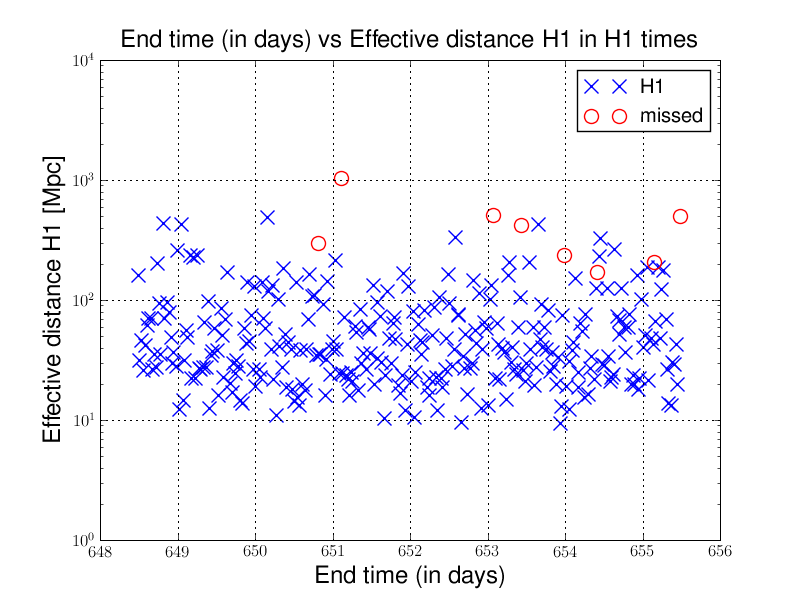
\includegraphics[width=0.5\linewidth]{figures/ninja2_results/h1-plotinspmissed_full_data_time-eff_dist-log-h1-871147524-606064.png}
  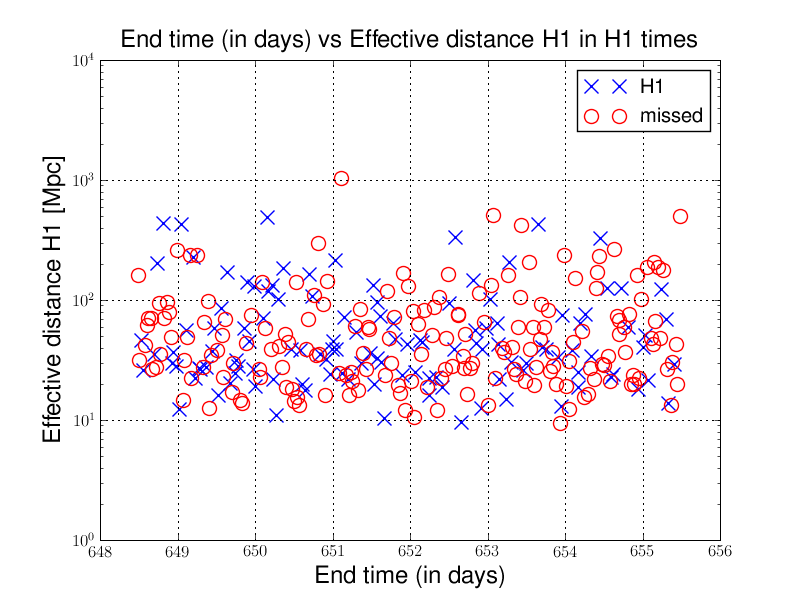
\includegraphics[width=0.5\linewidth]{figures/ninja2_results/h1-plotinspmissed_full_data_time-eff_dist-log-h1-871147524-606064_noiseonly.png} \\
  \caption[First-stage found/missed from the test data set]{
  \label{f:first_stage}
First-stage found/missed plots from the test data set.  On the left,
the results from the data set containing the injections, on the right
the results from running on the noise-only data.  Many signals appear
in both, indicating that they are not really found, but only that
there is a random background trigger within the time window.
}
\end{figure}%



\begin{figure}
  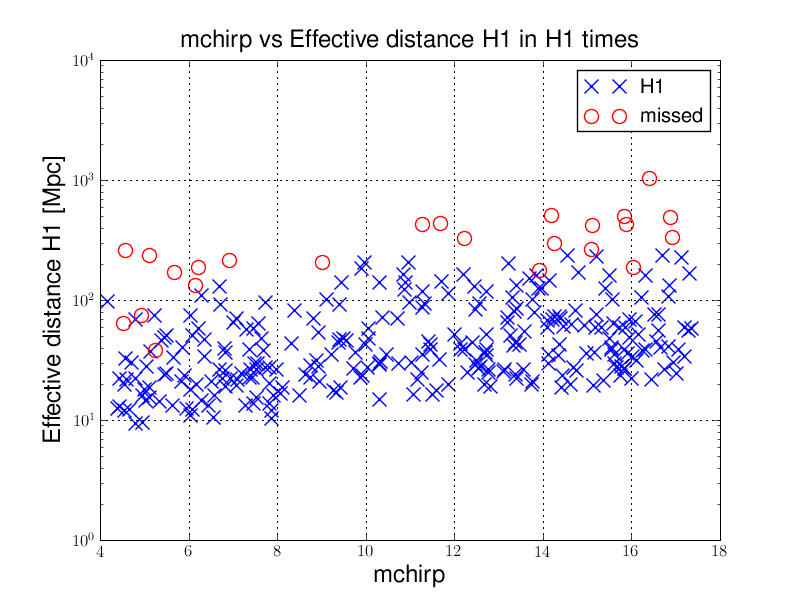
\includegraphics[width=0.5\linewidth]{figures/ninja2_results/h1-plotinspmissed_full_data_mchirp-eff_dist-log-h1-871147524-606064_second}
  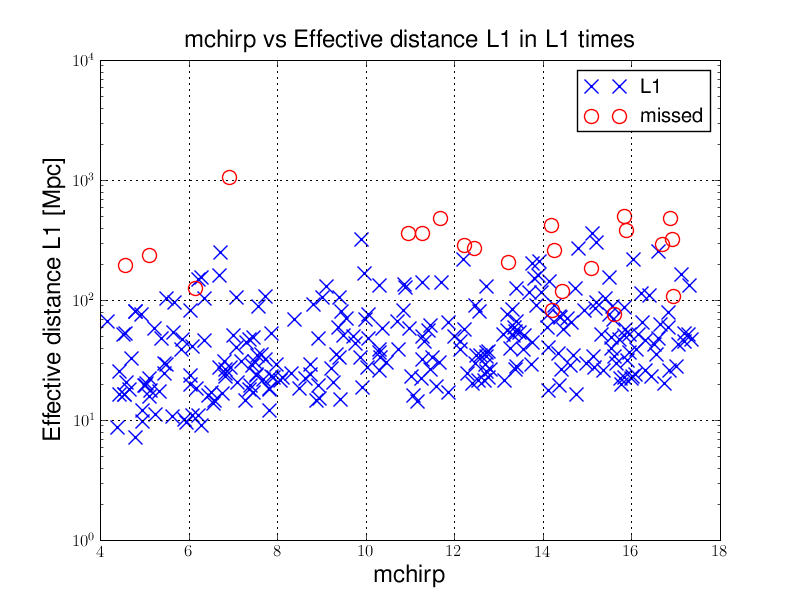
\includegraphics[width=0.5\linewidth]{figures/ninja2_results/l1-plotinspmissed_full_data_mchirp-eff_dist-log-l1-871147524-606064_second} \\
  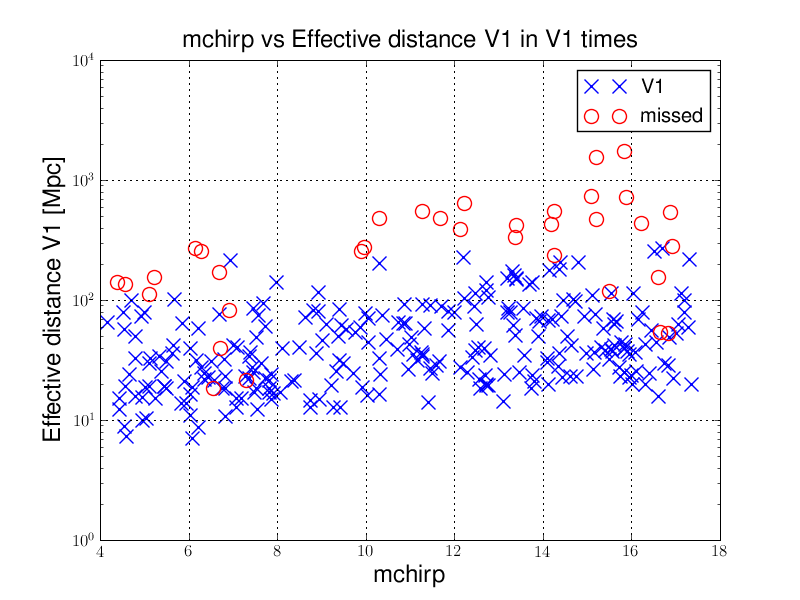
\includegraphics[width=0.5\linewidth]{figures/ninja2_results/v1-plotinspmissed_full_data_mchirp-eff_dist-log-v1-871147524-606064_second}
  \caption[Second-stage found-missed plots for the test data set]{
  \label{f:test_found_missed}
Second-stage found/missed plots for the test data set, for all three
detectors.  Each plot shows signals that were reovered in that
detector and at least one other.  Requiring coincidence removes the
background triggers seen in figure~\ref{f:first_stage}.  The results
are sensible: closer injections are more likely to be found than
distant ones.
}
\end{figure}%


In figure~\ref{f:test_recovered_snr} we plot the SNR recovered by the
pipeline versus the injected value.  There is a distinct pattern
exhibited, for low-mass signals the injected and recovered SNR match,
but the recovered SNR drops off with increasing mass.  This occurs
because the injected SNR value is calculated using the entire
waveform, taking the upper limit of the match filter to the Nyquist
frequency.  By contrast the recovered value terminates the integration
at the ISCO frequency.  For higher-mass systems this means the
integration cuts off in or before the sensitive band, while there is
still power in the signal, and consequently the SNR is underestimated.
While we can not hope to capture the full merger and ringdown with
inspiral-only templates, this again confirms the results of
chapter~\ref{ch:comparison} and NINJA-1, which show that extending the
templates to high frequencies can increase the SNR.

\begin{figure}
  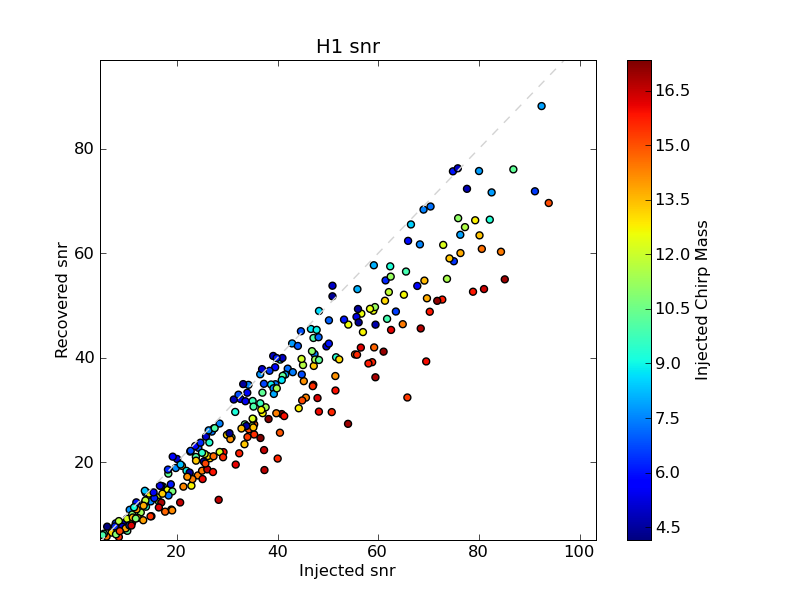
\includegraphics[width=0.5\linewidth]{figures/ninja2_results/h1_snrs_second}
  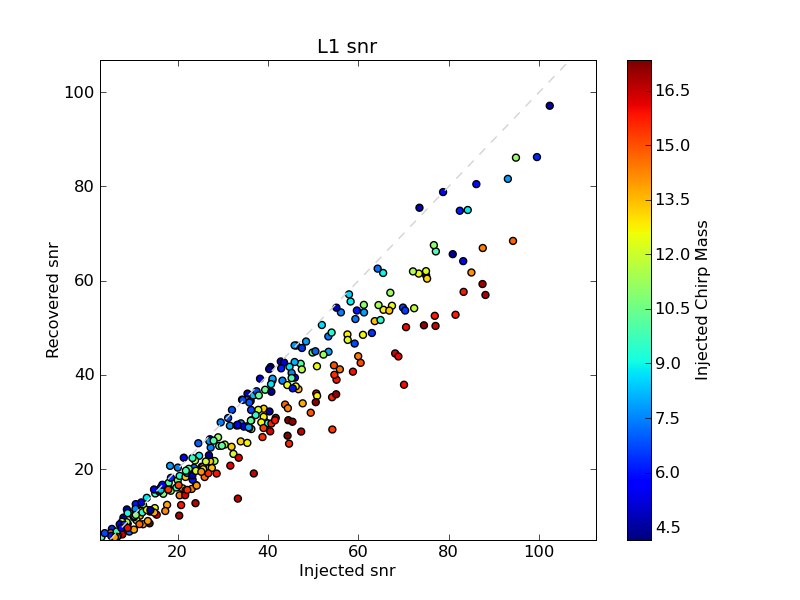
\includegraphics[width=0.5\linewidth]{figures/ninja2_results/l1_snrs_second} \\
  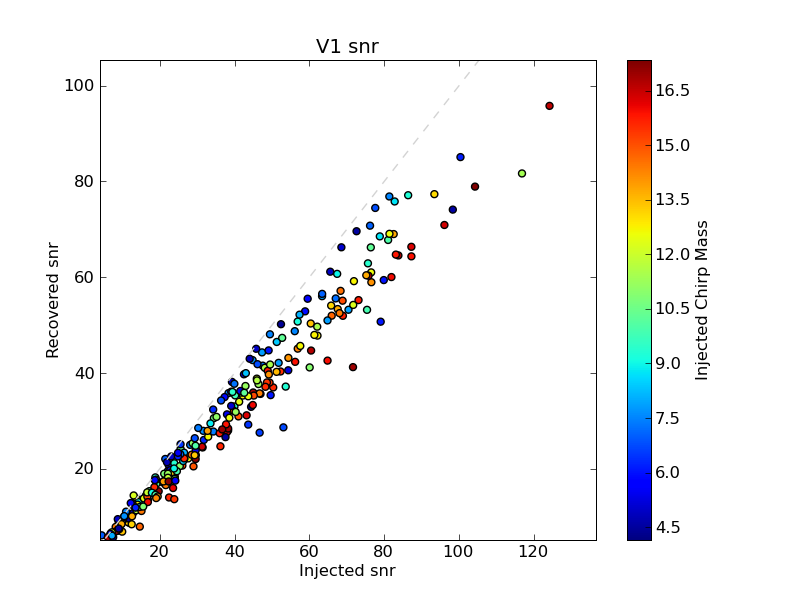
\includegraphics[width=0.5\linewidth]{figures/ninja2_results/v1_snrs_second}
  \caption[SNR recovery for the test data set]{
  \label{f:test_recovered_snr}
SNR recovery for the test data set in all three detectors.  The
injected SNR is calculated from the entire waveform, the recovered SNR
is calculated only from the inspiral up to the ISCO frequency.  At
higher masses this loses SNR as the late inspiral, merger, and
ringdown pass through the detector sensitive bands.  Note that V1,
which has lower noise at low frequencies, recovers somewhat more SNR
for the high-mass systems.
}
\end{figure}%


\iffalse
Can add if desired.
\begin{figure}
  \includegraphics[width=0.5\linewidth]{figures/ninja2_results/h1_masses_second}
  \includegraphics[width=0.5\linewidth]{figures/ninja2_results/l1_masses_second} \\
  \includegraphics[width=0.5\linewidth]{figures/ninja2_results/v1_masses_second}
  \caption[Mass recovery for the test data set]{
  \label{f:test_recovered_snr}
}
\end{figure}%
\fi

At the level of investigation performed the results from this data set
appear reasonable.  Although conversely this means that the waveform
truncation issue discussed above was not caught by this investigation.
However, this and other analyses did indicate that there were no other
more serious bugs in the injection software, which enabled us to move
to the full two-month set.

\section{CBC Results from the two-month data set}
\label{sec:ninjna2_two_months}

We now turn to the second two-month data set in Gaussian noise.  This
is the latest set constructed, and includes many corrections and
changes from earlier sets:

\begin{itemize}
\item The data is now sampled at 16,384 Hz.
\item There is now only one set spanning the full mass range from $10
\msun - 350 \msun$.
\item The waveforms have been updated, in particular many of the
hybridizations were redone.
\end{itemize}


Apart from the change in mass range the injection parameters were
chosen as described above.  The masses, spins, and distances chosen
are shown in figure~\ref{f:ninja2_dataset}.

\begin{figure}
  \includegraphics[width=\linewidth]{figures/ninja2_results/ninja2_dataset}
  \caption[Parameters of the NINJA-2 two-month data set]{
  \label{f:ninja2_dataset}
Distribution of mass, spin and distance parameters in the two-month,
Gaussian-noise data set.
}
\end{figure}%


\iffalse
Real detector data is far from Gaussian, and real data analysis is
concerned not only with foreground triggers from signals but also
background triggers from noise.  In order to comprehensively test the
ability of pipelines to detect signals and recover their parameters it
is necessary to perform injections into real detector noise.  As of
this writing a memorandum of understanding (MoU) between the NINJA
collaboration, the LIGO collaboration and the Virgo collaboration has
been signed which will allow subsequent NINJA-2 data sets to use data
from the previous (S5/VSR1) science run as noise.  A key feature of
this agreement is that NINJA is not a gravitational wave search.  We
will therefore use data from disjoint periods in each instrument.
Details of this plan, such as which times to use, have yet to be
decided.  However it is clear we will need a custom segment database
(see chapter~\ref{ch:detchar}) to mark times where the instruments
were glitching. However, injection times will not use this
information, as it is entirely possible that real signals will land on
or near a glitch, and the ability to detect such signals is an
important test.
\fi


This data set was analyzed with the standard CBC low-mass and
high-mass pipelines.  The parameters were exactly as in the S6/VSR2,3
runs, no changes were made to the configurations except for those
relating to the names of the data files.  The low-mass search uses
Taylor F2 templates to 3.5 pN order in phase evolution
(section~\ref{sec:PNWaveforms}) in a mass region defined by minimum
component masses of $1 \msun$ and maximum total mass of $25 \msun$.
The high mass search uses EOBNR templates (section~\ref{ssec:EOB}) in
a region defined by minimum component masses of $1 \msun$, minimum
total mass of $25 \msun$, and maximum total mass of $100 \msun$.


Figure~\ref{f:ninja2_cbc_results_high_first} shows the found/missed plots
after the first stage in the high-mass search.  As expected, distant
signals are less likely to be found than close ones.  As discussed
above the loose coincidence test between injections and triggers means
that many of these injections may not really be found.  We therefore
look at the second-stage results in
figure~\ref{f:ninja2_cbc_results_high_second}, and as in
figure~\ref{f:first_stage} there are many fewer found injections.  


\begin{figure}
  \includegraphics[width=0.5\linewidth]{figures/ninja2_results/H1-plotinspmissed_HIGH_FULL_DATA_mchirp-eff_dist-log-H1-871147552-5209912_first} 
  \includegraphics[width=0.5\linewidth]{figures/ninja2_results/L1-plotinspmissed_HIGH_FULL_DATA_mchirp-eff_dist-log-L1-871147552-5209912_first} \\
  \includegraphics[width=0.5\linewidth]{figures/ninja2_results/V1-plotinspmissed_HIGH_FULL_DATA_mchirp-eff_dist-log-V1-871147552-5209912_first} \\
  \caption[First stage found/missed plots from the high-mass search]{
  \label{f:ninja2_cbc_results_high_first}
Preliminary first stage found/missed plots from the high-mass search.
The behavior is as expected: distant signals are more likely to be
missed than close ones.
}
\end{figure}%

\begin{figure}
  \includegraphics[width=0.5\linewidth]{figures/ninja2_results/H1-plotinspmissed_HIGH_FULL_DATA_mchirp-eff_dist-log-H1-871147552-5209912_first} 
  \includegraphics[width=0.5\linewidth]{figures/ninja2_results/L1-plotinspmissed_HIGH_FULL_DATA_mchirp-eff_dist-log-L1-871147552-5209912_first} \\
  \includegraphics[width=0.5\linewidth]{figures/ninja2_results/V1-plotinspmissed_HIGH_FULL_DATA_mchirp-eff_dist-log-V1-871147552-5209912_first} \\
  \caption[Second stage found/missed plots from the high-mass search]{
  \label{f:ninja2_cbc_results_high_second}
Preliminary second stage (after coincidence and $\chisq$) found/missed plots from
the high-mass search.  As expected, many of the signals reported as
``found'' after the first stage were due to background triggers within
100 ms of the injection.  More signals are missed at higher masses
because the high-mass bank only extends to $100 \msun$ but there are
injections up to $350 \msun$.  There is an anomaly in the Virgo
results, see the text for discussion.
}
\end{figure}%

The fraction of injections found decreases with increasing mass.  The
bank of the high-mass search extends only to $100 \msun$, but the
injections extend up to $350 \msun$, so this result is not surprising.
We can quantify the effect by plotting the efficiency, defined as this
fraction, as a function of mass.  These plots are shown in
figure~\ref{f:high_mass_efficiencies}.  While these plots show the
general trend, they are quite jagged, indicating that we do not have
enough injections to draw statistical conclusions.  Follow up work
will remedy this by performing many thousands of ``on the fly''
injections.

There is an unexpected feature in the V1 plot, which shows that at
high mass more close injections are missed than distant ones.  We
will return to this issue below.


\begin{figure}
  \includegraphics[width=0.5\linewidth]{figures/ninja2_results/H_second_mass_high_efficiency}
  \includegraphics[width=0.5\linewidth]{figures/ninja2_results/L_second_mass_high_efficiency} \\
  \includegraphics[width=0.5\linewidth]{figures/ninja2_results/V_second_mass_high_efficiency}
  \caption[Efficiency of the high-mass pipeline as a function of mass]{
  \label{f:high_mass_efficiencies}
Efficiencies of the high-mass pipeline as a function of mass.  As
can be seen in figure ~\ref{f:ninja2_cbc_results_high_second} the
efficiencies decrease as mass increases.  However, the jaggedness in
these plots indicates that there are not enough injections to draw
definitive conclusions.
}
\end{figure}%

The standard CBC low-mass and high-mass searches both use non-spinning
templates, and an important question is the ability of these pipelines
to detect spinning signals.  NINJA-2 is uniquely positioned to help
answer this question, and we begin by plotting the recovery efficiency
of the high-mass pipeline as a function of the spin parameter $\chi$
in figure~\ref{f:high_spin_efficiencies}.  There is a general trend
suggesting that the efficiency increases with $\chi$, and in
particular that the search performs worse on anti-aligned systems than
aligned systems.  Again, the jaggedness of the plots makes it
impossible to draw definitive conclusions, but this will be remedied in
follow up studies with more injections.



\begin{figure}
  \includegraphics[width=0.5\linewidth]{figures/ninja2_results/H_second_spin_high_efficiency}
  \includegraphics[width=0.5\linewidth]{figures/ninja2_results/L_second_spin_high_efficiency} \\
  \includegraphics[width=0.5\linewidth]{figures/ninja2_results/V_second_spin_high_efficiency}
  \caption[Efficiency of the high-mass pipeline as a function of mass]{
  \label{f:high_spin_efficiencies}
Efficiencies of the high-mass pipeline as a function of the spin
parameter $\chi$.  There is a general trend suggesting the pipeline
is more efficient at detecting aligned spins, but more injections are
needed to verify and quantify this.
}
\end{figure}%


We now consider the parallel analysis performed with the low-mass
search.  Figure~\ref{f:ninja2_cbc_results_low_first} shows the
found/missed plots after the first stage.  Again, distant signals are
more likely to be missed than close ones.  The low-mass template bank
extends to a total mass of $25\msun$, and correspondingly the
efficiency decreases notably above a chirp mass of $\approx 80 \msun$.

The anomalous behavior in Virgo is more pronounced here than in the
high-mass search, with most injections above a chirp mass of $100
\msun$ and closer than $100$ Mpc being missed.  We return to this
issue in section~\ref{ssec:virgo_anomaly}.

Figure~\ref{f:ninja2_cbc_results_low_second} shows the found/missed
plots after the second stage.  Again, many of the injections reported
as found in the first stage are now reported as missed.  The remaining
found injections are clustered towards the low end of the mass range,
as expected.  However, in all IFOs at this stage the remaining found
injections at higher masses tend to be at further distances, contrary
to the expected behavior.  In addition, the injections found in V1 are
mostly confined to the region $M_{chirp} < 20 \msun$, whereas those in
H1 and L1 extend up to $\approx 60 \msun$.  This indicates that most
of triggers above $20 \msun$ are found in coincidence between H1 and
L1.  In turn this implies that signals above this point are either not
really found in V1 at the first stage, or are seen with very different 
parameters that fail the coincident test with the H1 and L1 triggers.
Again we defer further discussion to section~\ref{ssec:virgo_anomaly}.


\begin{figure}
  \includegraphics[width=0.5\linewidth]{figures/ninja2_results/H1-plotinspmissed_LOW_FULL_DATA_mchirp-eff_dist-log-H1-871147552-5209912_first} 
  \includegraphics[width=0.5\linewidth]{figures/ninja2_results/L1-plotinspmissed_LOW_FULL_DATA_mchirp-eff_dist-log-L1-871147552-5209912_first} \\
  \includegraphics[width=0.5\linewidth]{figures/ninja2_results/V1-plotinspmissed_LOW_FULL_DATA_mchirp-eff_dist-log-V1-871147552-5209912_first} \\
  \caption[First stage found/missed plots from the low-mass search]{
  \label{f:ninja2_cbc_results_low_first}
Preliminary first stage found/missed plots from the low-mass search.
The behavior is as expected: distant signals are more likely to be
missed than close ones.
}
\end{figure}%

\begin{figure}
  \includegraphics[width=0.5\linewidth]{figures/ninja2_results/H1-plotinspmissed_LOW_FULL_DATA_mchirp-eff_dist-log-H1-871147552-5209912_first} 
  \includegraphics[width=0.5\linewidth]{figures/ninja2_results/L1-plotinspmissed_LOW_FULL_DATA_mchirp-eff_dist-log-L1-871147552-5209912_first} \\
  \includegraphics[width=0.5\linewidth]{figures/ninja2_results/V1-plotinspmissed_LOW_FULL_DATA_mchirp-eff_dist-log-V1-871147552-5209912_first} \\
  \caption[Second stage found/missed plots from the low-mass search]{
  \label{f:ninja2_cbc_results_low_second}
Preliminary second stage found/missed plots from
the low-mass search.  Virgo appears to only find injections below a
chirp mass of $20 \msun$, all found injections above this point come
from coincidences between H1 and L1.  In all IFOs injections found at
higher masses have larger effective distances.  Further studies are
needed to understand this behavior, see
section~\ref{ssec:virgo_anomaly}.
}
\end{figure}%

The efficiencies of the pipeline as a function of mass is shown in
figure~\ref{f:low_mass_efficiencies}, and as a function of spin in
figure~\ref{f:low_spin_efficiencies}.  The mass plots present the
same information found in figure~\ref{f:ninja2_cbc_results_low_second}
in an alternate way, and as in the corresponding high-mass plots
indicate that more injections are needed in order to refine the
results.  The spin plots show the same general trend in the high-mass
plots, again indicating that the search is more efficient at detecting
systems with aligned spins than anti-aligned.

\begin{figure}
  \includegraphics[width=0.5\linewidth]{figures/ninja2_results/H_second_mass_low_efficiency}
  \includegraphics[width=0.5\linewidth]{figures/ninja2_results/L_second_mass_low_efficiency} \\
  \includegraphics[width=0.5\linewidth]{figures/ninja2_results/V_second_mass_low_efficiency}
  \caption[Efficiency of the low-mass pipeline as a function of mass]{
  \label{f:low_mass_efficiencies}
Efficiencies of the low-mass pipeline as a function of mass.  As
can be seen in figure~\ref{f:ninja2_cbc_results_low_second} the
efficiencies decrease as mass increases.  However, the jaggedness in
these plots indicates that there are not enough injections to draw
definitive conclusions.
}
\end{figure}%

\begin{figure}
  \includegraphics[width=0.5\linewidth]{figures/ninja2_results/H_second_spin_low_efficiency}
  \includegraphics[width=0.5\linewidth]{figures/ninja2_results/L_second_spin_low_efficiency} \\
  \includegraphics[width=0.5\linewidth]{figures/ninja2_results/V_second_spin_low_efficiency}
  \caption[Efficiency of the low-mass pipeline as a function of spin]{
  \label{f:low_spin_efficiencies}
Efficiencies of the low-mass pipeline as a function of the spin
parameter $\chi$.  There is a general trend suggesting the pipeline
is more efficient at detecting aligned spins, but more injections are
needed to verify and quantify this.
}
\end{figure}%


\subsection{Anomalous Virgo results}
\label{ssec:virgo_anomaly}

In both the high-mass and low-mass searches we find that at higher
chirp masses closer injections are missed while further injections are
found.  This problem is evident in all three interferometers, but it
is most extreme in Virgo and affects even the first-stage results.  At
the time of writing no explanation for this behavior has yet been
found, however some possibilities have been ruled out.  As the problem
is most notable in Virgo we focus attention there.

First, we consider the possibility that the effective distance is
simply being misreported.  We check this by plotting the injections on
the same axes as the found/missed plots, color-coding by injected SNR.
This is shown in figure~\ref{f:anomaly_snrs}, which shows that the SNR
and effective distance, which are calculated by different portions of
the code, correlate.  This rules out this possibility.

\begin{figure}
  \includegraphics[width=\linewidth]{figures/ninja2_results/anomaly_snrs}
  \caption[Injections color-coded by SNR]{
  \label{f:anomaly_snrs}
Injections plotted as in the found/missed plots, color-coded by SNR.
If high SNRs corresponded to points found in Virgo it would indicate
that the effective distances were being miscalculated.  However, this
is not the case.
}
\end{figure}%

We next consider the possibility of a correlation between effective
distance and total mass.  These values are chosen randomly and
independently, but if there were some correlation such that high
effective distances corresponded to lower total masses it would
explain the results by indicating that more distant injections
happened to be more likely to fall within the range of the bank.
We again plot the injections as in the found/missed plots, now
color-coding by total mass, in figure~\ref{f:anomaly_masses}.  Again,
no correlations are seen.


\begin{figure}
  \includegraphics[width=\linewidth]{figures/ninja2_results/anomaly_snrs}
  \caption[Injections color-coded by total mass]{
  \label{f:anomaly_masses}
Injections plotted as in the found/missed plots, color-coded by total
mass.  If lower masses corresponded to points found in Virgo it would 
indicate a correlation between effective distance and mass.  However, this
is not the case.
}
\end{figure}%

Finally, we examine in detail one of the injections with chirp mass
above $100 \msun$ that is found in Virgo at the first stage beyond 100
Mpc, looking for any indication that the time series are badly
behaved.  Figure~\ref{f:anomaly_time_series} shows the injection, the
filtered data, and the SNR time series arranged so that they all cover
the same two-second interval.  All three line up as expected, at the
level of this test this injection seems to be found legitimately.

\begin{figure}
  \includegraphics[width=0.5\linewidth]{figures/ninja2_results/signal}
  \includegraphics[width=0.5\linewidth]{figures/ninja2_results/filtered}
  \includegraphics[width=\linewidth]{figures/ninja2_results/snr}
  \caption[Time series of an distant injection found in V1]{
  \label{f:anomaly_time_series}
Time series plots of an injection found in Virgo,  chirp mass $135
\msun$ at 157 Mpc.  Top left shows the scaled waveform.  Top right
shows the data segment passed to the matched filter,
after bandpassing to reduce low-frequency noise.  Bottom shows the SNR
time series.  All plots line up as expected.
}
\end{figure}%


\section{Open Questions for NINJA-2}

Beyond resolving the unexplained behavior in the searches we intend to
use NINJA-2 to address several important open question.  We briefly
note these here.

\weakheader{Further tests of the pipeline modifications}

We intend to rerun these analyses using a bank extended to unphysical
$\eta$ and terminating the waveforms at the WRD frequency, as in
NINJA-1.  The goal is to determine how this affects the efficiency of
the search at lower masses than could be tested in NINJA-1, as well as
on a wider range of parameter space.  We will also repeat the analysis
in real detector noise.  A critical question is how the extended bank
will affect the rate of background triggers.  NINJA-1 indicates we can
recover higher SNRs by making this change, but if this comes with an
elevated background, making signals stand out less strongly, then this
change will not be useful.

\weakheader{Transition between the low-mass and high-mass searches}

The dividing line between the low- and high-mass searches is somewhat
arbitrary at present.  We hope to use efficiency plots such as those
presented in this chapter, populated with many more injections, to
determine the point at which the efficiencies cross.  In particular,
as will be discussed in the next chapter, much of the background in
the low-mass search comes from the higher-mass end of the template
bank.  If we can reduce the upper limit of the low-mass search we can
hope to clean up the background and make quiet signals more
significant.

\weakheader{Effects of spin}

Using efficiency plots such as those presented in this chapter we hope
to determine the regions of parameter space that are not well-covered
by the existing non-spinning searches.  Such regions could then be
supplemented by spinning searches currently in development.
Conversely, by identifying regions where the current search performs
adequately we can limit the range, and hence the background, over
which spinning searches need to run.

\weakheader{Effects of template placement}

As discussed in section~\ref{sec:bank_metric}, the current searches
use a bank laid out according to a metric calculated from the Taylor
F2 stationary-phase waveform taken to 2.0 pN order in phase.  Current
searches use 3.5 pN waveforms, and the template placement is therefore
incorrect.  The extent to which it is incorrect, and the implications
for the search, can be tested by running \emph{bank simulations}.  In
such a simulation a bank is constructed and the maximum overlap
between a signal and every template in the bank is found.  By
comparing this maximum against the maximum found by varying the
parameters continuously (as in chapter~\ref{ch:comparison}) we can
determine the loss in SNR due to discretizing  the bank.  We plan to
run such analyses using the NINJA-2 signals with both 2.0 pN templates
and 3.5 pN templates in order to determine the extent to which the
incorrect metric decreases the efficiency of the search.

\section{Conclusions}

In this chapter we discussed the NINJA-2 data sets and presented
results from a one-week test run on a data set containing only low
mass signals, and a two-month set containing signals up to $350
\msun$.  The test week shows no anomalies, however when the mass range
is extended the low-mass pipeline shows unexpected behavior.  We
consider a few possibilities to explain this, but as of this writing
no explanation has been found.  It seems more likely to be a bug in
the data set generation than in the analysis, as the latter has been
much more extensively reviewed.  In either case, more study is needed.




\Chapter{A Database for Instrumental Data Quality}
\label{ch:segdb}

\subsection{Data Quality Flags}

The state of the instrument at any time is summarized by a set of
\emph{flags}.  Flags are identified by a triple of (ifo id, flag name,
version number), where \emph{ifo id} identifies the instrument,
\emph{flag name} is a unique identifier, and \emph{version number} is
an integer starting from 1.  The version number allows information to
be updated without losing information that may be needed to
reconstruct the results of earlier searches.  The full set of flags is
stored in a database designed at Syracuse and hosted at Caltech.

Flags are stored as a set of \emph{segments}, half-open intervals
aligned on GPS integer second boundaries.  Each flag triple has an
associated set of segments indicating the times during which it is
\emph{defined}.  Such triples also have a set of segments indicating
times during which they are \emph{active}.  The set of active segments
must be a subset of defined segments.  Times during which a flag is
defined and not active are considered \emph{inactive}.

Flags may be entered manually through a web interface.  This can be
used to indicate nonstandard operating conditions, such as heavy
equipment being operated on site.  However, most flags are generated
automatically.

The first line of defense against noise triggers is on-site as the
instrument is running.  At all such times the control room is staffed
by an operator who is an expert in running the instrument employed by
LIGO labs, and a science monitor (``SciMon'') who is a member of the
LIGO Scientific Collaboration.  The two jointly decide when to enable
\emph{science mode}, which marks the data as suitable for analysis.
This declaration is not specific to the CBC group, but extends to all
searches in the collaboration.  Science time is indicated by the flag
\texttt{DMT\_SCIENCE}.

In addition to the readout channel (\texttt{DARM\_ERR}, section
\ref{sec:inst_readout} many other data channels are recorded, falling
into two broad categories.  Physical environmental monitor (``PEM'')
channels record information about the environment such as seismic
activity at the base and end stations, microphones and magnetometers
placed throughout the site, etc.  Instrumental (``INST'') channels
record data from numerous subsystems such as servos for each mirror
and the output of photodiodes at points throughout the light path.
Software running at the sites called the data monitoring tool
(``DMT'') creates data quality flags based on these channels.  For
example, when a channel's value or standard deviation over time
exceeds a given threshold.  The DMT is also responsible for recording
the state of the science mode flag.  Other flags are set by programs
that run analyses on these auxiliary channels, for examples see
(\checkme{UPV refs}).


\subsection{The Veto Definer}

Problems in the data may have differing levels of severity, and
consequently we define several \emph{veto categories} to characterize
them.  The categories used by daily ihope differ slightly from those
used by the full analysis.

Category 1 vetoes indicates time that should not have been marked as
science mode.  Typically attempting to analyze this time will
adversely affect the entire 2048-second analysis chunk, for example by
biasing the PSD (section \ref{sec:ihope_psd}).  Note that it is
possible to correct science time by creating a new version of the
\texttt{DMT\_SCIENCE} flag with an incremental version number.
However, doing so is a more complicated process than creating a veto
flag, and removing time by denoting it CAT1 carries additional
information about the reason for the veto.  Note that category 1
vetoes are undesirable, as they may remove time outside the range of
the problem.  For example, a 4080-second span of science-mode data
with a one-second CAT1 veto at 2040 seconds will be completely
unanalyzable by the CBC group, as excising the bad data will leave no
contiguous 2048-second block.

Category 2 vetoes indicates time during which there was a problem,
instrumental or environmental, with well-understood coupling into
\texttt{DARM\_ERR}.  Such time can be analyzed without problem, but
triggers from such time will be discarded. 

Category 3 vetoes remove hardware injections (section
\ref{sec:ihope_hardware_injections}).  In the full analysis hardware
injectiob vetos do not have a category number and is denoted
``hardware injections removed.''

Category 4 is for time that appears to be ill-behaved according to 
data quality studies, but where there is no clearly-understood 
cause.  In the full analysis this is denoted category 3.

Finally, a map is needed between data quality flags and veto
categories.  This is achieved through the use of a search-specific
\emph{veto definer file} which associates a flag with a veto level.
Intervals within the range during which that version of the flag are
active will be marked with the corresponding veto level.  The
\texttt{ligolw\_segments\_from\_cats} program (see below) merges the
information in this file with the set of active flag segments to produce
\emph{veto segments} at each veto level.  Analysis is performed on
times marked as science with no CAT1 vetoes.  Triggers from times
marked as CAT2, CAT3 and CAT4 are discarded from both foreground and
background.

Sometimes the threshold on a DQ flag is such that the data is
unsuitable for analysis close to, but outside, the range of the flag.
The veto definer file therefore allows for \emph{padding}, offsets 
which effectively extend the flags.


\subsection{Technical details}

The flag segments are stored in a high-performance relational
database, exposed as a web service which provides secure access to all
members of the collaboration.  Several utilities to interact with the
segment database were written, many of which could run in many modes.
The names of all these utilities start with ligolw, short for ``LIGO
lightweight,'' an XML-based format used throughout the collaboration
in which the output was generated.

Except where noted all programs accept a common subset of arguments
\begin{itemize}
\item \texttt{--gps-start-time} and \texttt{--gps-end-time}: Integer
GPS times specifying the time range over which to run.
\item \texttt{--include-segments}: Takes a comma-separated list of
segment specifiers of the form ifo:flag\_name:version or
ifo:flag\_name and restricts the query to matching flags.  In the
latter case, report on the latest version of the flag defined at each
time within the time range.
\item \texttt{--exclude-segments}: Takes a comma-separated list of
segment specifiers in the same format as \texttt{--include-segments}.
Runs a second query on the excluded segments and returns the set of
segments in included segments - (included segments $\cap$ excluded
segments).
\item \texttt{--database}, \texttt{--segment-url},
\texttt{--dmt-files}: Specifies the data source (segment database or
XML files with segment information).
\end{itemize}


The programs used during S6 were:

\textbf{ligolw\_dq\_query}.  This program reports on the state of
flags at one or more GPS times given on the command line.  This
program does not support \\
\texttt{--gps-start-time} or \texttt{--gps-end-time}.   The available modes are

\begin{itemize}
\item \texttt{--report}:  Returns the active/inactive status of all DQ flags at the
given times.  For active flags reports the start and end times of the
segment within which the given time is contained.  For inactive flags
reports the end time of the nearest preceding segment and the start
time of the nearest subsequent segment.  This mode is used in the
daily ihope ``loudest glitches'' page, see below.
\item \texttt{--defined}: Returns a list of flags defined at the
given times.
\item \texttt{--active}: Returns a list of the flags that were active
at the given times.
\item \texttt{--start-pad}, \texttt{--end-pad}: Extends the
\texttt{--defined} and \texttt{--active} modes to report on the status
of flags within a small range of time.
\end{itemize}


\textbf{ligolw\_segment\_query}.  This program reports on the state of a
set of flags over a span of times.  The available modes are

\begin{itemize}
\item \texttt{--show-types}: Reports the sets of flags that exist over
the time span.
\item \texttt{--query-types}: Reports the segments during which the
flags were defined.
\item \texttt{--query-segments}: Reports the segments during which the
flags were active.
\end{itemize}

Every CBC analysis begins by determining the science mode times with a
call of the form

\vspace*{5mm}
\texttt{ligolw\_segment\_query} \\
\hspace*{0.5in}\texttt{--query-segments --include-segments H1:DMT-SCIENCE:3 ...}
\vspace*{5mm}

\textbf{ligolw\_segments\_from\_cats}.  Given a veto definer file,
report on segments to be vetoed. 

\textbf{ligolw\_dq\_active\_cats}.  Given a veto definer file and GPS
time, report on the active/inactive status and veto category for all
flags defined at the time.

\textbf{ligolw\_segment\_insert}.  Adds new segments to the database,
enforcing various policy decisions:
\begin{itemize}
\item New segments for an existing flag/version number pair must not overlap 
with existing segments.  To update information a new version number must be used.
\item New version numbers must be one greater than the largest
existing version number.
\item New segments must not extend into the future, past the GPS time
at which the program is run.
\end{itemize}


% https://www.lsc-group.phys.uwm.edu/daswg/wiki/content_of_segment_publication_and_discovery

\Note{Following taken from T0900005 -- Needs to be integrated!}


%%%%%%%%%%%%%%%%%%%%%%%%%%%%%%%%%
\section{Introduction}

This document describes the infrastructure used to manage data quality
and veto information in the LIGO S6 Science Run. Data quality
information is generated by a combination of automated Data Monitoring
Tool (DMT) software and scientist investigation. This information must
be stored for archiving and retrieval. A suite of tools should be
provided for users to update and query the stored data. In S6, the
segment database is the central location all DQ data is written in to. 

Two parallel solutions are being pursued:
\begin{enumerate}
\item A database-based solution will allow users to store and query segment
information. This will be based on the infrastrure used in S5, updated with
the lessons learned from the science run.
\item Tools will be provided to allow users/programs to query the online DQ
data files generated by the DMT. This will allow users to perform small
low-latency queries relevant to online searches in the most direct manner
possible.
\end{enumerate}

\section{Implementation plan}
\begin{figure}[h]
  \begin{center}
    \includegraphics[width=0.9\linewidth]{figures/segdb/T0900005_fig1}
  \end{center}
  \caption{Data flow for S6 data quality segment information. Online data
  quality segments and science segment information is generated by the DMT.
  This can be directly queried for low-latency online analysis or inserted
  into a segment database for off-line or higher-latency analyses. Command
  line and web GUI  tools can be used to query and update the segment
  database.} 
\end{figure}

\begin{enumerate}
\item \textbf{DMT trigger manager:} The DMT trigger manager will handle the
creation of all science segments and online data quality segments in S6. Every
60 seconds, the DMT trigger manager writes segment information in XML format
to disk at the Observatories. The DMT calls the \verb|dmtdq_seg_insert|
program to insert the XML data into the segment database.

To prevent confusion with cases sensitivity in processing tools, all DQ flag
names must be in upper case case. Additionally, a 3-letter prefix will be
added to each DQ flag to better identify the source where data comes from. For
example: the S5 DQ flag known as \verb|Wind_Over_30MPH| should be writted
into the XML file as \verb|DMT-WIND_OVER_30MPH| in S6. All DQ flags generated online by the DMT should have version
number 1.

\item \textbf{Archival of DMT segment data:} The 60 second XML files generated
by the DMT will be archived every 3600 seconds onto the LDAS
\verb|/archive/dataprods| filesystem for replication to Caltech and Teir 2
computing centers. Files will be compressed using the gzip algorithm.

\item \textbf Software will be developed to take the XML files from DMT disk
and together with a data quality categorization file managed by the search
groups (e.g. H1-ONLINEALLSKYBURSTCATS-815155200-63072000.xml) will produce XML
files containing the segments for a given DQ category for a given search once
per minute or so. In addition ligolw\_print can be used to convert these XML
files to ASCII format for search groups that want ASCII segment lists. The same
software will be made available for interfacing with the segment database for
offline searches and detector characterization. 

\item \textbf{Expected Latencies:} as described in the implementation plan
diagram, expected latencies are:
\begin{itemize}
\item DMT generates h(t) file: 60 seconds
\item From DMT to raw DMT segment disk: 60 seconds
\item From raw DMT segment disk to segment database: 10 seconds
\item From ligolw\_segment\_insert to segment database: 30 seconds
\end{itemize}
\end{enumerate}



%%%%%%%%%%%%%%%%%%%%%%%%%%%%%%%%%%%%%%%%%%%%%%%%
\section{S6 segment database design}

The S6 segment database schema (and hence the XML files) have been
substantially simplified for S6.  The five tables to be used for S6 are shown
in figure~\ref{f:schema}. All uncessary tables have been eliminated and the
remaining table set simplified. The \verb|process|, \verb|process_params| and
\verb|segment_definer| tables are unchanges from S5, with the exception that
the \verb|domain| column in the \verb|process| table is used to store the
distingished name of the user inserting the data.  In S5, segments were either
stored as on or off allowing users to distinguish between a segment being off
or undefined, due to data not being analyzed. It was foung that the
off/undefined query was used substantially less than the on query, and so in
S6 this column is eliminated from the \verb|segment| table.  To ensure that
off/undefined information is still available, the a \verb|segment_summary| is
introduced in S6 to store time intervals when quality flags are defined. This
further simplified the query ``What versions were defined at what time?''
allowing better use of version information in S6.

\begin{figure}[h]
  \begin{center}
    \includegraphics[width=0.9\linewidth]{figures/segdb/T0900005_fig3}
  \end{center}
  \label{f:schema}
  \caption{S6 Segment Database Schema}
\end{figure}





%%%%%%%%%%%%%%%%%%%%%%%%%%%%%%%%%%%%%%%%%%%%%%%%
\section{Data Replication Between Observatories and Tier 2 Centers}

In S6, Caltech segment database is the official data repository. In
addition to being written into the database, all data inserted in to
the Caltech segment database will be output as xml files to a central
location. These xml files will then be replicated to tier 2 sites at
ldas.ligo-wa.caltech.edu, ldas.ligo-la.caltech.edu. A rsync script
will be implemented at Caltech to periodically replicate xml files
from Caltech to tier 2 sites. At the sites, a publishing script will
be implemented to publish the xml files to the local segment database.

In addition to database replication, the archived DMT segment files will be
replicated between sites using rsync, according to the DASWG
\verb|/archive/dataprods| prototcol.


%%%%%%%%%%%%%%%%%%%%%%%%%%%%%%%%%%%%%%%%%%%%%%%%%
\section{User Interface}

\subsection{GUI Segment Query Tools}

In S6, we will no longer support plain ASCII dumps of the segment database.
Use of segwizard will be depricated in favor of a web-based GUI, similar to
the web GUI used by the Virgo segment database.  Users will be able to
manipulate graphical tools in the web browser interface to retrieve desired
results directly from the segment database. 

A GUI will also be provided for the DetChar chair (and designated people) to
modify segment information stored in the database.

\subsection{Command Line Tools}

\subsubsection{ligolw\_segment\_query}

The glue program \verb|ligolw_segment_query| replaces LSCsegFind as the
command line interface to query for data quality and science segments.
\verb|ligolw_segment_query| can query either the segment database or
directories containing XML segment files generated by the DMT.
\verb|ligolw_segment_query| only provides read access to the segment database.
\verb|ligolw_segment_query| primarily intended for human interaction with the
segment database. Automated generation of DQ files for online searches should
use the program \verb|ligolw\_veto\_segments|.

Below are the questions that ligolw\_segment\_query can answer:
\begin{itemize}
\item What DQ flags exist in the database? ligolw\_segment\_query --show-types
\item When was a given flag inserted? ligolw\_segment\_query --query-types
\item When was a given DQ flag defined? ligolw\_segment\_query --query-types
\item When was a given flag active? ligolw\_segment\_query --query-segments 
\end{itemize}


DESCRIPTION:
{\small
\begin{verbatim}
  --version             show program's version number and exit
  -h, --help            show this help message and exit
  -p, --ping            Ping the target server
  -y, --show-types      Returns a xml table containing segment type
                        information: ifos, name, version,
                        segment_definer.comment, segment_summary.start_time,
                        segment_summary.end_time, segment_summary.comment
  -u, --query-types     Returns a ligolw document whose segment_definer table
                        includes all segment types defined in the given period
                        and included by include-segments and whose
                        segment_summary table indicates the times for which
                        those segments are defined.
  -q, --query-segments  Returns a ligolw document whose segment table contains
                        the times included by the include-segments flag and
                        excluded by exclude-segments
  -s gps_start_time, --gps-start-time=gps_start_time
                        Start of GPS time range
  -e gps_end_time, --gps-end-time=gps_end_time
                        End of GPS time range
  -t segment_url, --segment-url=segment_url
                        Segment URL. Users have to specify either 'https://'
                        for a secure connection or 'http://' for an insecure
                        connection in the segment database url. For example,
                        '--segment-url=https://segdb.ligo.caltech.edu'. No
                        need to specify port number.
  -d, --database        use database specified by environment variable
                        S6_SEGMENT_SERVER. For example,
                        'S6_SEGMENT_SERVER=https://segdb.ligo.caltech.edu'
  -f, --dmt-files       use files in directory specified by environment
                        variable ONLINEDQ, for example,
                        'ONLINEDQ=file:///path_to_dmt'. 'file://' is the
                        prefix, the acutal directory to DMT xml files starts
                        with '/'.
  -a include_segments, --include-segments=include_segments
                        This option expects a comma separated list of a colon
                        separated sublist of interferometer, segment type, and
                        version. The union of segments from all types and
                        versions specified is returned. Use --show-types to
                        see what types are available.   For example:
                        --include-segment-types H1:DMT-SCIENCE:1,H1:DMT-
                        INJECTION:2 will return the segments for which H1 is
                        in either SCIENCE version 1 or INJECTION version 2
                        mode. If version information is not provided, the
                        union of the segments of the latest version of
                        requested segment type(s) will be returned.
  -b exclude_segments, --exclude-segments=exclude_segments
                        This option has to be used in conjunction with
                        --include-segment-types --exclude-segment-types
                        subtracts the union of unwanted segments from the
                        specified types from the results of --include-segment-
                        types. If version information is not provided,
                        --exclude-segment-types subtracts the union of
                        segments from the latest version of the specified
                        segment types. For example, --include-segment-types H1
                        :DMT-SCIENCE:1,H1:DMT-INJECTION:2 --exclude-segment-
                        types H1:DMT-WIND:1,H1:DMT-NOT_LOCKED:2,H2:DMT-
                        NOT_LOCKED:2 will subtract the union of segments which
                        H1 is in version 1 WIND and H1,H2 is version 2
                        NOT_LOCKED from the result of --include-segment-types
                        H1:DMT-SCIENCE:1,H1:DMT-INJECTION:2
  -S, --strict-off      The default behavior is to truncate segments so that
                        returned segments are entirely in the interval [gps-
                        start-time, gps-end-time).  However if this option is
                        given, the entire non-truncated segment is returned if
                        any part of it overlaps the interval.
  -o output_file, --output-file=output_file
                        File to which output should be written.  Defaults to
                        stdout.
\end{verbatim}
}

\subsubsection{ligolw\_dq\_query}
ligolw\_dq\_query can query either the segment database or directories containing XML segment files generated by the DMT. ligolw\_dq\_query only provides read access to the segment database. 

Below are the questions that ligolw\_dq\_query can answer:
\begin{itemize}
\item is a given flag active at a given time? ligolw\_dq\_query --active
\item is a given flag defined at a given time? ligolw\_dq\_query --defined
\item what is the status of all flags at a given time? ligolw\_dq\_query --report
\end{itemize}


DESCRIPTION:
{\small
\begin{verbatim}
  --version             show program's version number and exit
  -h, --help            show this help message and exit
  -p, --ping            Ping the target server
  -y, --defined         Returns a segment summary table containing segments
                        defined at the given time(s).
  -u, --active          Returns a segment table containing segments active at
                        the given time(s).
  -q, --report          Prints which flags are defined/undefined at the given
                        time(s). For the flags which were defined, it
                        determines if the flag was active or inactive at that
                        time. For an active flag, it prints the start and end
                        time of the segment to which the active. For an
                        inactive flag, it prints the end time of the previous
                        adjacent active segment and the start time of the next
                        adjacent active segment
  -s start_pad, --start-pad=start_pad
                        Seconds before given time(s) to include in query
  -e end_pad, --end-pad=end_pad
                        Seconds after given time(s) to include in query
  -t segment_url, --segment-url=segment_url
                        Segment URL
  -d, --database        use database specified by environment variable
                        S6_SEGMENT_SERVER
  -f, --dmt-files       use files in directory specified by environment
                        variable ONLINEDQ
  -a include_segments, --include-segments=include_segments
                        This option expects a comma separated list of a colon
                        separated sublist of interferometer, segment type, and
                        version. The union of segments from all types and
                        versions specified is returned. Use --show-types to
                        see what types are available.   For example:
                        --include-segment-types H1:SCIENCE:1,H1:INJECTION:2
                        will return the segments for which H1 is in either
                        SCIENCE version 1 or INJECTION version 2 mode. If
                        version information is not provided, the union of the
                        segments of the latest version of requested segment
                        type(s) will be returned.
  -o output_file, --output-file=output_file
                        File to which output should be written.  Defaults to
                        stdout.
  -i, --in-segments-only
                        If set, report will only return segments that given
                        times were within
\end{verbatim}
}



\subsubsection{ligolw\_segments\_from\_cats}
ligolw\_segments\_from\_cats reads one or more segment files and a veto file and generates files of veto segments.

DESCRIPTION:
\begin{verbatim}
  --version             show program's version number and exit
  -h, --help            show this help message and exit
  -v veto_file, --veto-file=veto_file
                        veto XML file (required).
  -o output_dir, --output-dir=output_dir
                        Directory to write output (default=cwd).
  -k, --keep-db         Keep sqlite database.
  -t segment_url, --segment-url=segment_url
                        Segment URL
  -d, --database        use database specified by environment variable
                        S6_SEGMENT_SERVER
  -f, --dmt-file        use files in directory specified by environment
                        variable ONLINEDQ
  -c, --cumulative-categories
                        If set the category N files will contain all segments
                        in categories <= N
  -p, --separate-categories
                        If set the category N files will contain only category
                        N
  -s gps_start_time, --gps-start-time=gps_start_time
                        Start of GPS time range
  -e gps_end_time, --gps-end-time=gps_end_time
                        End of GPS time range
\end{verbatim}


For example:
\begin{verbatim}
ligolw\_segments\_from\_cats --gps-start-time 930960015 --gps-end-time 931564887 --segment-url https://segdb.ligo.caltech.edu:30015 --cumulative-categories --veto-file http://www.lsc-group.phys.uwm.edu/ligovirgo/cbc/public/segments/S6/H1L1V1-S6\_CBC\_LOWMASS\_ONLINE-928271454-0.xml
\end{verbatim}




\subsubsection{ligolw\_segment\_insert}
ligolw\_segment\_insert is the replacement of LSCdqInsert. ligolw\_segment\_insert handles two tasks:
\begin{itemize}
\item Insert segments and/or segment types into the segment database.
\item Append segments to the existing segment types.
\end{itemize}
ligolw\_segment\_insert follows the underlying methods of LSCdqInsert to insert segments, but there are several changes made in ligolw\_segment\_insert which includes:
\begin{itemize}
\item - -interval option is removed. In LSCdqInert, - -interval is used to read in a single segment. With ligolw\_segment\_insert, user has to specify a plain text file containing the segment(s), even if there is only one segment in the text file.
\item - -run option is removed.
\item Users have to provide segment file which contains the active segments of a given segment type of the whole run and summary file which contains the validity intervals of this given segment type of the whole run which activ segments belong.
\end{itemize}

DESCRIPTION:
\begin{verbatim}
  -h, --help            show this help message and exit
  -p, --ping            Ping the target server
  -t URL, --segment-url=URL
                        Users have to specify protocol 'https://' for a secure
                        connection in the segment database url. For example,
                        '--segment-url=https://segdb.ligo.caltech.edu'. No
                        need to specify port number'.
  -o FILE, --output=FILE
                        Write segments to FILE rather than the segment
                        database
  -j IDENTITY, --identity=IDENTITY
                        Set the subject line of the server's service
                        certificate to IDENTITY
  -I, --insert          Insert segments to the segment database
  -A, --append          Append segments to an existing segment type
  -i IFOS, --ifos=IFOS  Set the segment interferometer to IFOS (e.g. H1)
  -n NAME, --name=NAME  Set the name of the segment to NAME (e.g. DMT-
                        BADMONTH)
  -v VERSION, --version=VERSION
                        Set the numeric version of the segment to VERSION
                        (e.g. 1)
  -e EXPLAIN, --explain=EXPLAIN
                        Set the segment_definer:comment to COMMENT. This
                        should explaining WHAT this flag mean (e.g. "Light dip
                        10%"). Required when --Insert/-I is specified.
  -c COMMENT, --comment=COMMENT
                        Set the segment_summary:comment to COMMENT. This
                        should explaining WHY these segments were inserted
                        (e.g. "Created from hveto results")
  -S FILE, --summary-file=FILE
                        Read the segment_summary rows from FILE. This should
                        be a file containing the gps start and end times that
                        the flag was defined, deliminated by comma (i.e. the union of on and off)
  -G FILE, --segment-file=FILE
                        Read the segment rows from FILE. This should containin
                        the gps start and end times when the flag was active deliminated by comma
\end{verbatim}

To insert segments of new segment type, the command would look like:
\begin{verbatim}
ligolw\_segment\_insert --segment-url https://segdb.ligo.caltech.edu --ifos 'H1' --name 'DCH-TEST' --version 1 --comment 'testing if insert works' --explain 'test insert' --segment-file segment.txt --summary-file summary.txt --insert
\end{verbatim}

To append segments to an existing segment, the command would look like:
\begin{verbatim}
ligolw\_segment\_insert --segment-url https://segdb.ligo.caltech.edu --ifos 'H1' --name 'DCH-TEST' --version 1 --comment 'testing if append works' --segment-file append_segment.txt --summary-file append_summary.txt --append
\end{verbatim}
%%%%%%%%%%%%%%%%%%%%%%%%%%%%%%%%%%%%%%%%%%%%%%%%%%
\section{Functionality Supported in S6}
With the above described web browser and command line user interface, users will be able to find out:
\begin{itemize}
\item When was a given flag defined?
\item Was a given flag defined at this time?
\item When was a given flag active?
\item What is the dead time for a given flag? 
\item At a given point of time, is the given flag active? If yes, find out the start and end time of the segment to which the specified point of time belongs.
\item At a given point of time, is the given flag active? If no, find out the end time of the previous adjacent active segment and the start time of the next adjacent active segment.
\item Provide the same supports described above for a set of flags.
\item What flags were active at this time, near this time ($\pm 1$~s interval or specified by user)?
\item What is the efficiency for a flag for burst and inspiral and plot it.
\item Export answer to ascii or xml file
\item Handle padding windows for deadtime queries
\item Export config files, start, end times
\end{itemize}


%%%%%%%%%%%%%%%%%%%%%%%%%%%%%%%%%%%%%%%%%%%%%%%%%
\section{Authentication}
In S6, data insertion requires authentication. Retrieving from on-site requires no authentication. Retrieving from off-site requires authentication. 

\section{Exchange of data with Virgo}

\section{Example Veto Configuration File}

The veto configuration file should contain a \verb|process| table describing
how it was created and a \verb|veto_definer| table describing the flags to be
applied at different levels. The comment column of the process table should
contain the version of the file. The columns in the \verb|veto_definer| table
are as follows: \verb|ifo|, \verb|name| and \verb|version| uniquely define a
particular DQ/veto flag. \verb|category| described which veto category it
should be applied at (i.e. $0, 1, 2, 3, \ldots$), \verb|start_time| and
\verb|end_time| denote the GPS time interval for which the DQ/veto flag should
be applied (Note: if \verb|end_time| is zero, then the current GPS time is
assumed). \verb|start_pad| and \verb|end_pad| are the padding time (in
seconds) applied to the start and end of the veto segments. Note that these
are signed: if you want time vetoed to start time to be \emph{earlier} than
the start time listed in the database, then the emph \verb|start_pad| should
be \emph{negative}. Similarly, if the time vetoed should extend \emph{after}
the end time stored in the database, then the value in \verb|end_pad| should
be \emph{positive}. The \verb|comment| column can be used to store an optional
human-readable comment.

{\tiny
\begin{verbatim}
<?xml version='1.0' encoding='utf-8' ?>
<!DOCTYPE LIGO_LW SYSTEM "http://ldas-sw.ligo.caltech.edu/doc/ligolwAPI/html/ligolw_dtd.txt">
<LIGO_LW>
   <Table Name="process:table">
      <Column Name="process:process_id" Type="ilwd:char"/>
      <Column Name="process:program" Type="lstring"/>
      <Column Name="process:version" Type="lstring"/>
      <Column Name="process:cvs_repository" Type="lstring"/>
      <Column Name="process:cvs_entry_time" Type="int_4s"/>
      <Column Name="process:node" Type="lstring"/>
      <Column Name="process:username" Type="lstring"/>
      <Column Name="process:unix_procid" Type="int_4s"/>
      <Column Name="process:start_time" Type="int_4s"/>
      <Column Name="process:end_time" Type="int_4s"/>
      <Column Name="process:ifos" Type="lstring"/>
      <Column Name="process:comment" Type="lstring"/>
      <Stream Name="process:table" Type="Local" Delimiter=",">
      "process:process_id:0","ligolw_veto_file","1.1",
      "/usr/local/cvs/lscsoft/glue/bin/ligolw_veto_file,v",822908378,
      "ldas-grid.ligo.caltech.edu","jrsmith",16830,822879594,822879594,
      "H1","Example file by Josh"
      </Stream>
   </Table>
   <Table Name="veto_definer:table">
      <Column Name="veto_definer:process_id" Type="ilwd:char"/>
      <Column Name="veto_definer:ifo" Type="lstring"/>
      <Column Name="veto_definer:name" Type="lstring"/>
      <Column Name="veto_definer:version" Type="int_4s"/>
      <Column Name="veto_definer:category" Type="int_4s"/>
      <Column Name="veto_definer:start_time" Type="int_4s"/>
      <Column Name="veto_definer:end_time" Type="int_4s"/>
      <Column Name="veto_definer:start_pad" Type="int_4s"/>
      <Column Name="veto_definer:end_pad" Type="int_4s"/>
      <Column Name="veto_definer:comment" Type="lstring"/>
      <Stream Name="veto_definer:table" Type="Local" Delimiter=",">
      "process:process_id:0","H1","OUT_OF_LOCK",0,1,917985615,0,0,0,"",
      "process:process_id:0","H1","BADGAMMA",1,1,917985615,0,0,0,"",
      "process:process_id:0","H1","ASC_Overflow",0,2,917985615,0,-8,8,"ASC saturations are cat2",
      "process:process_id:0","H1","PD_Overflow",0,2,917985615,0,-8,8,"PD saturations are cat2",
      "process:process_id:0","H1","SEVERE_LSC_OVERFLOW",0,2,917985615,0,-8,8,"LSC saturations are cat2",
      "process:process_id:0","H1","INJECTION",1,2,917985615,0,-16,64,"Remove HW injections at cat1",
      "process:process_id:0","H1","ASC_Overflow",0,3,917985615,0,-8,25,"ASC saturations are cat3 with larger pad",
      "process:process_id:0","H1","SEVERE_LSC_OVERFLOW",0,3,917985615,0,-8,25,"LSC saturations are cat3 with larger pad",
      "process:process_id:0","H1","PD_Overflow",0,3,917985615,0,-8,25,"PD saturations are cat3 with larger pad",
      "process:process_id:0","H1","Wind_over_30MPH",0,3,917985615,0,-8,8,"Windy",
      "process:process_id:0","H1","LIGHTDIP_1_PERCENT",0,3,917985615,0,-2,2,"Exclude all lightdip segments",
      "process:process_id:0","H1","PRE_LOCKLOSS_10_SEC",0,3,917985615,0,0,0,"",
      "process:process_id:0","H1","PRE_LOCKLOSS_30_SEC",0,3,917985615,0,0,0,"",
      "process:process_id:0","H1","PRE_LOCKLOSS_60_SEC",0,3,917985615,0,0,0,"",
      "process:process_id:0","H1","PRE_LOCKLOSS_120_SEC",0,3,917985615,0,0,0,"",
      "process:process_id:0","H1","ASI_CORR_OVERFLOW",0,4,917985615,0,-8,25,"Does this make sense for DC readout",
      "process:process_id:0","H1","LSC_OVERFLOW",0,4,917985615,0,-8,25,"LSC saturations",
      "process:process_id:0","H1","PRE_LOCKLOSS_600_SEC",0,4,917985615,0,0,0,"",
      "process:process_id:0","H1","PRE_LOCKLOSS_1800_SEC",0,4,917985615,0,0,0,""
      </Stream>
   </Table>
</LIGO_LW>
\end{verbatim}
}

\section{Segment Data File}

To be ingested into the segment database, segment data to be must be in the
format described in this section. Data should be in a valid LIGO LW XML file
with \verb|process|, \verb|segment_definer|, \verb|segment_summary| and
\verb|segment| tables. An optional \verb|process_params| table can be used to
store extra metadata about segment generation.

The \verb|process| table should contain the columns given in the XML file
below which describe the name, version, cvs repository and revision of the
program used generate the data. The comment column can be used to add
additional human-readable data. The node, username, unix\_procid, start\_time
and end\_time columns should store metadata describing who ran the process and
where it ran. The ifos column should contain an alphabetical list of all ifo
data using as input to the process. The process\_id column is used to link the
defined process to other rows in the file created by that process.

The \verb|segment_definer| table should contain a definition of the segments
included in the file. The ifos, name and version column should contain the
name and version of the segment. The name should be upper case for all
segments. DMT-derived segments should be prefixed with the string \verb|DMT-|,
KleineWelle derived veto segments should be prefixed with the string
\verb|KWV-|, data derived from the detector state vector channels should be
prefixed with \verb|IFO-|, segments created by the detchar group should be
prefixes with \verb|DCH-| and segments from the Virgo database should be
prefixed with \verb|VDB-|.  The comment column can be used to add a
human-readable description of the segment. The segment\_definer columm is used
to link this type of segment to the intervals in the \verb|segment| and
\verb|segment_summary| tables.

The \verb|segment| table should contain the GPS start and end time when the
segment described in the \verb|segment_definer| table was \emph{active}. The 
\verb|segment_summary| table should contain the GPS start time and end time of
the interval for which the segment is \emph{defined}. This will allow users to
distinguish between the cases where a DQ segment is undefined for a particular
time or simply inactive (i.e. it is \emph{not} windy, as opposed to the wind
monitor being down).

{\tiny
\begin{verbatim}
<?xml version="1.0"?>
<!DOCTYPE LIGO_LW SYSTEM "http://ldas-sw.ligo.caltech.edu/doc/ligolwAPI/html/ligolw_dtd.txt">
<LIGO_LW>
  <Table Name="processgroup:process:table">
    <Column Name="processgroup:process:program" Type="lstring"/>
    <Column Name="processgroup:process:version" Type="lstring"/>
    <Column Name="processgroup:process:cvs_repository" Type="lstring"/>
    <Column Name="processgroup:process:cvs_entry_time" Type="int_4s"/>
    <Column Name="processgroup:process:comment" Type="lstring"/>
    <Column Name="processgroup:process:node" Type="lstring"/>
    <Column Name="processgroup:process:username" Type="lstring"/>
    <Column Name="processgroup:process:unix_procid" Type="int_4s"/>
    <Column Name="processgroup:process:start_time" Type="int_4s"/>
    <Column Name="processgroup:process:end_time" Type="int_4s"/>
    <Column Name="processgroup:process:process_id" Type="ilwd:char"/>
    <Column Name="processgroup:process:ifos" Type="lstring"/>
    <Stream Name="processgroup:process:table" Type="Local" Delimiter=",">
      "SegGener","1.17",
      "/ldcg_server/common/repository_gds/gds/Monitors/SegGener/SegGener.cc\,v",
      865755895,"Segment generation from an OSC condition","granite","jzweizig",718,
      918756928,918836992,"process:process_id:0","H0H1H2"
    </Stream>
  </Table>
  <Table Name="segment_definergroup:segment_definer:table">
    <Column Name="segment_definergroup:segment_definer:process_id" Type="ilwd:char"/>
    <Column Name="segment_definergroup:segment_definer:segment_def_id" Type="ilwd:char"/>
    <Column Name="segment_definergroup:segment_definer:ifos" Type="lstring"/>
    <Column Name="segment_definergroup:segment_definer:name" Type="lstring"/>
    <Column Name="segment_definergroup:segment_definer:version" Type="int_4s"/>
    <Column Name="segment_definergroup:segment_definer:comment" Type="lstring"/>
    <Stream Name="segment_definergroup:segment_definer:table" Type="Local" Delimiter=",">
      "process:process_id:0","segment_definer:segment_def_id:35","H2","DMT-LIGHT",1,
      "H2 Light in arms from h(t) DQ flags",
      "process:process_id:0","segment_definer:segment_def_id:36","H2","DMT-SCIENCE",1,
      "H2 Science mode from h(t) DQ flags",
      "process:process_id:0","segment_definer:segment_def_id:37","H2","DMT-INJECTION",1,
      "H2 Injection mode from h(t) DQ flags",
      "process:process_id:0","segment_definer:segment_def_id:38","H2","DMT-UP",1,
      "H2 calibration OK in from h(t) DQ flags",
      "process:process_id:0","segment_definer:segment_def_id:39","H2","DMT-CALIBRATED",1,
      "H2 Calibration OK from h(t) DQ flags",
      "process:process_id:0","segment_definer:segment_def_id:40","H2","DMT-BADGAMMA",1,
      "H2 Bad gamma in h(t) DQ flags"
    </Stream>
  </Table>
  <Table Name="segmentgroup:segment:table">
    <Column Name="segmentgroup:segment:segment_id" Type="ilwd:char"/>
    <Column Name="segmentgroup:segment:start_time" Type="int_4s"/>
    <Column Name="segmentgroup:segment:end_time" Type="int_4s"/>
    <Column Name="segmentgroup:segment:segment_def_id" Type="ilwd:char"/>
    <Column Name="segmentgroup:segment:process_id" Type="ilwd:char"/>
    <Stream Name="segmentgroup:segment:table" Type="Local" Delimiter=",">
      "segment:segment_id:15",918836961,918836977,"segment_definer:segment_def_id:35",
      "process:process_id:0",
      "segment:segment_id:16",918836976,918836992,"segment_definer:segment_def_id:37",
      "process:process_id:0"
    </Stream>
  </Table>
  <Table Name="segment_summarygroup:segment_summary:table">
    <Column Name="segment_summarygroup:segment_summary:segment_sum_id" Type="ilwd:char"/>
    <Column Name="segment_summarygroup:segment_summary:start_time" Type="int_4s"/>
    <Column Name="segment_summarygroup:segment_summary:end_time" Type="int_4s"/>
    <Column Name="segment_summarygroup:segment_summary:comment" Type="lstring"/>
    <Column Name="segment_summarygroup:segment_summary:segment_def_id" Type="ilwd:char"/>
    <Column Name="segment_summarygroup:segment_summary:process_id" Type="ilwd:char"/>
    <Stream Name="segment_summarygroup:segment_summary:table" Type="Local" Delimiter=",">
      "segment_summary:segment_sum_id:5",918836976,918836992,"",
      "segment_definer:segment_def_id:40","process:process_id:0",
      "segment_summary:segment_sum_id:6",918836976,918836992,"",
      "segment_definer:segment_def_id:39","process:process_id:0",
      "segment_summary:segment_sum_id:11",918836976,918836992,"",
      "segment_definer:segment_def_id:37","process:process_id:0",
      "segment_summary:segment_sum_id:12",918836976,918836992,"",
      "segment_definer:segment_def_id:35","process:process_id:0",
      "segment_summary:segment_sum_id:42",918836976,918836992,"",
      "segment_definer:segment_def_id:36","process:process_id:0",
      "segment_summary:segment_sum_id:46",918836976,918836992,"",
      "segment_definer:segment_def_id:38","process:process_id:0"
    </Stream>
  </Table>
</LIGO_LW>
\end{verbatim}
}

\section{Converting XML to plain ASCII}
ligolw\_print can be used to convert XML file to plain ASCII format. ligolw\_print prints the contents of table elements from one or more LIGO Light Weight XML files to stdout in delimited ASCII format.  In addition to regular files, the
program can read from many common URLs such as http:// and ftp://.  Any filename or URL that ends in ".gz" is assumed to be gzip-compressed, and will be decompressed on input.  If no filenames or URLs are given, then input is read from stdin.


DESCRIPTION:
\begin{verbatim}
  --version             show program's version number and exit
  -h, --help            show this help message and exit
  -i name, --input-cache=name
                        Get URLs from the LAL cache file.  Can be provided
                        multiple times to name several caches to iterate over.
  -c name, --column=name
                        Print only the contents of the given column.  Can be
                        provided multiple times to print multiple columns.
                        The default is to print all columns from each table.
  -d string, --delimiter=string
                        Delimit output with the given string.  The default is
                        ",".
  -r rowspec, --rows=rowspec
                        Print rows in the given range(s).  The format is
                        first:last[,first:last,...].  Rows are numbered from
                        0.  A single first:last pair requests rows in the
                        range [first, last).  If the first or last value of a
                        pair is omited it means 0 or infinity respectively.
                        The default is ":", or to print all rows.
  -t name, --table=name
                        Print rows from this table.  Can be provided multiple
                        times to print rows from multiple tables.  The default
                        is to print the contents of all tables.
  -a name, --array=name
                        Print the contents of this array.  Can be provided
                        multiple times to print the elements from multiple
                        arrays.  The default is to print the contents of all
                        arrays.
  -v, --verbose         Be verbose.
  --constrain-lsc-tables
                        Impose additional constraints on official LSC tables.
                        Provides format validation and allows RAM requirements
                        to be reduced.
\end{verbatim}



\Chapter{Characterization of a Gravitational Wave Detector}
\label{ch:detchar}
As discussed in section \ref{sec:ihope_far}, the CBC group measures
the significance of candidate events by comparing the combined new SNR
(sec.~\ref{sec:search_new_snr}) against the background distribution.
The background is obtained by sliding the triggers from each IFO
against each other by more than the light travel time between them.
In the limit of at most one real gravitational wave in each analysis
segment this ensures that the background is composed entirely of
triggers resulting from non- gravitational-wave sources.

Ideally, the instrumental noise would be Gaussian and the only source
of extraneous triggers would be random fluctuations.  In reality
environmental couplings to the instrument, such as electrical and
seismic, as well as glitches within the instrument will also produce
triggers.

It is in the interest of the collaboration to remove as many of these
triggers as possible so that any real events will stand out 
well above the background.  This removal must be done in
an automated way in advance of looking at the results from the
analysis.  LIGO would be justly criticized if the background were
to be adjusted after the analysis in order to make a marginal candidate
appear more significant.

There is therefore a need for a process of detector characterization
(henceforth ``detchar''), a way to remove times from the analysis that
are more likely to produce triggers from noise than from a real event.
One of the most significant features of the S6 run is that the people
working on detchar were in close contact with the people commissioning
the instrument.  This meant that, in addition to cleaning the search,
information about problematic behavior in the instrument could be used
to fix the problems at the source, in turn allowing more time to be
analyzed and the prospects for making a detection to improve.

Detchar was a major undertaking, much more information can be found in
(Smith and Lundgren in progress).  Here we focus on the \emph{segment
database}, a key piece of infrastructure, and \emph{daily ihope}, a
modification of the CBC search used for detchar.


\section{Daily ihope}


As discussed in (search chapter) the CBC group uses the \emph{ihope}
pipeline to search for gravitational waves produced by the inspiral of
binary systems consisting of neutron stars and/or black holes.  During
LIGO's 6th science run (July 7, 2009 - October 20, 2010) which
overlapped Virgo's second (July 7, 2009 - January 11, 2010), and third
(August 11, 2010 - October 20, 2010) science runs, the goal of the
group was to run the full analysis every two weeks with latencies as
small as possible.  The daily ihope runs were conceived of as a way to
characterize the detector in order to look for potential problems in
advance of the full search, particularly problems specific to the CBC
search.

It is important to stress that daily ihope was not itself a
gravitational wave search, it was a tool to help determine whether the
data in each instrument was suitable to analyze.  This goal determined
the specifics of the daily runs, but more significantly it leaves the
full search unbiased.

Recall that ihope is a templated, matched-filter search.  For the
low-mass search, which was the focus of the daily runs, the templates
are restricted, stationary-phase frequency-domain waveforms with phase
evolution taken to 3.5 PN order.  The templates are laid out in a bank
with 97\% overlap between nearest neighbors, and the mass range is
from 2 $\msun - 25 \msun$.  A $\chisq$ discriminator is constructed to
better separate signals from glitches (eqn \ref{eq:analysis_chisq} ,
and the information from this discriminator is used along with the SNR
to construct the new SNR detection statistic (eqn
\ref{eq:analysis_newsnr}).

By construction a great deal of the information provided by
the full bank search is redundant.  Further, the evaluation of each
additional template and the initial layout of the bank incurs
significant computational overhead.  Therefore a number of
simplifications were applied to the daily ihope bank.

First, a static bank was used for each IFO, based on the layout at a
quiet time in each instrument.  Second, the number of templates was
reduced.  Lower-mass systems have more cycles in the sensitive LIGO
band, there is therefore ample information to distinguish between
waveforms with close parameters.  Conversely, this means that the
low-mass end of the bank is very dense (in the sense of number of
templates per unit square in parameter space, they are still
equidistant in the sense of eq. \ref{eq:analysis_match_filter}).  Such
fine resolution is not needed when looking for glitches, therefore the
minimal match between templates in the region below a chirp mass
($\mathcal{M} = M \eta^{3/5}$) of 3.46 $M_\odot$ was set to 0.5.  At
higher masses, up to a total mass of $25 M_\odot$, the minimal match
was set to 0.95.  In addition to ensuring coverage in a mass region
which is naturally sparser this ensures that short glitches,
characteristic of many glitch mechanisms, were flagged with large
SNRs.  The resulting hybrid bank for the Hanford detector is shown in
figure \ref{f:daily_ihope_bank}.

\begin{figure}
  \includegraphics[width=\linewidth]{figures/detchar/hybrid_bank.png}
  \caption[The hybrid template bank used by daily ihope]{
  \label{f:daily_ihope_bank}
The hybrid template bank used by daily ihope for the Hanford detector,
the banks for L1 and V1 are similar.
The cut is made at constant chirp mass, which is
a curve in the total mass, $\eta$ plane.}
\end{figure}%

Daily ihope processing ran at 03:00 GMT and examined data spanning the
24 hours ending at 00:00 GMT.  Unlike full ihope, the analysis was
done on all science time, including that which would be vetoed at CAT
1 by the full analysis.  This was done so that we could see the effect
of the CAT 1 vetoes.  It is plausible, for example, that some such
vetoes would be too aggressive and we could decide based on the daily
results to include such times back into the analysis.  For consistency
science time was denoted CAT 0.  In addition CAT 3 vetoes to remove
hardware injections were not applied, so that we could see how many
injections would be lost by CAT 4 vetoes.  The daily pages therefore
displayed results for categories 0, 1, 2, and 4.

For each 2048-second chunk of contiguous data, at each IFO, the data
was run through each template in the bank and triggers selected as
described in section \ref{sec:analysis_trigger_selection}. For each
trigger $\chisq$ and new SNR were calculated and recorded.  Clustering
was then done in order to focus attention on glitches that were most
likely to cause problems in the full search.  Two sets of clustered
triggers were recorded using windows of 30 milliseconds and 16
seconds.  For each set the trigger with the largest value of new SNR
across all templates within the window length was recorded.

The triggers were also filtered.  A version of the veto definer file
designated as ``online'' was maintained and used by daily ihope to
identify times with veto categories.  These vetoed times were then
removed from the original and clustered files.  
% The pipeline is summarized in figure (xx).
The result is, for each 2048-second block in each ifo, 3 cluster
levels times 4 veto levels = 12 sets of triggers.

%do analysis
%record science triggers
%cluster 30 ms     determine cat 1
%cluster 16 sec    determine cat 1 + cat 2
%                  ...

%filter and record

\section{The Daily Ihope report pages}

Much of the utility of the daily runs was in the use of the resulting
triggers to identify data quality issues and quantify the value of
proposed vetoes.  Some of these uses will be discussed in
section~\ref{sec:applications}.  In addition to the triggers the daily
pipeline also produced a large number of plots and reports, organized
into web pages that were available to the collaboration.  Data
analysts could use these pages to spot potential problems for the full
analysis and begin more detailed followup studies.  

We now summarize the contents of the daily pages. Each report and plot
is made for each combination of the following:

\begin{itemize}
\item IFO: H1, L1 and V1
\item Cluster level: Unclustered, 30 ms clustering, 16 second
clustering
\item Veto level: Show all triggers in science time (level ``0''),
only those not removed by category 1 vetos, only those not
removed by categories 1 or 2, or only those note removed by
categories 1,2 and 4.  Hardware injections vetos (category 3) were not 
applied so that we could determine whether category 4 vetoes were 
remove them.
\end{itemize}

Each of these features could be set independently.  The top-level web
interface for a sample day is shown in figure~\ref{f:daily_ihope_top}.

\begin{figure}
  \includegraphics[width=\linewidth]{figures/detchar/daily_ihope_top}
  \caption[Top-level web interface for daily ihope]{
  \label{f:daily_ihope_top}
Top-level web interface for daily ihope.  Options can be selected with
the controls on the left hand side, when a button is clicked the
contents region is immediately replaced.  The default view is the one
shown here; the analysis time and veto efficiency at cat 1 for the
Hanford detector.}
\end{figure}%

The available reports can bee seen at the bottom of the list of
controls in figure~\ref{f:daily_ihope_top}:


1. Analysis time and veto usage.  This report shows the total time
analyzed, the vetoes applied beyond those applied at the previous
level, the \emph{efficiency} (percentage of triggers removed) and
\emph{deadtime} (percentage of time removed) by each veto.  In
addition the ratio of efficiency over deadtime is reported as a
measure of quality of the veto.  A random veto would result in an
efficiency-over-deadtime of approximately 1, a finely-tuned veto that
removes short, loud events that ring off the entire template bank
would have a much higher ratio.   An example is shown in
figure~\ref{f:daily_ihope_vetousage}.


\begin{figure}
  \includegraphics[width=\linewidth]{figures/detchar/vetousage.png}
  \caption[Sample veto usage report from Aug 19, 2010]{
  \label{f:daily_ihope_vetousage}
A sample veto usage report, see text for explanation.  Note that 62.66\% of
all triggers were contained in 14.51\% of time, and the DMT flagged this time
with elevated seismic activity from 3-10 Hz at the LVEA.}
\end{figure}%

2. Loudest triggers.  This report was only run for 16-second-clustered
triggers.  Loud glitches tend to produce families of triggers, without
clustering the loudest triggers from each day would likely result from
one underlying event.  This report considers two classes of triggers;
those where no data quality flag was active and those where at least
one flag was active.  A sample report is shown in
figure~\ref{f:daily_ihope_loudest}.  For the five triggers with
highest new SNR in each category a summary was presented along with a
link to an \emph{omega scan}.  The omega pipeline is described in
(\checkme{omega refs}).  Omega scans are a kind of time-frequency
plot.  They are especially useful as they may be run on all auxiliary
channels recorded by the instruments and therefore provide a visual
aid to detecting coupling between auxiliary channels and the
gravitational wave readout channel.  These can be used to suggest
mechanisms behind glitches, especially those that were not already
marked by a DQ flag.  In addition, over time repeated shapes in the
omega scan can pinpoint underlying problems in the instruments that
need to be addressed.  A few images from one of the glitches in
figure~\ref{f:daily_ihope_loudest} is shown in
figure~\ref{f:daily_ihope_loudest_omega}.

\begin{figure}
  \includegraphics[width=\linewidth]{figures/detchar/loudest.png}
  \caption[Sample loudest trigger report from Aug 19, 2010]{
  \label{f:daily_ihope_loudest}
A sample report on loudest triggers, see text for explanation.  Note the
rightmost column is populated by
the \texttt{ligolw\_dq\_query} program in the \texttt{--report} mode.}
\end{figure}%



\begin{figure}
  \includegraphics[width=0.5\linewidth]{figures/detchar/966222827_940673828_H1_LSC-DARM_ERR_1_00_spectrogram_whitened.png}
  \includegraphics[width=0.5\linewidth]{figures/detchar/966222827_940673828_H0_PEM-ISCT1_ACCX_1_00_spectrogram_whitened.png}
  \caption[Omega scans from the loudest H1 trigger in figure \ref{f:daily_ihope_loudest}]{
  \label{f:daily_ihope_loudest_omega}
Omega scans from the loudest H1 trigger in figure
\ref{f:daily_ihope_loudest}.
Note the trigger closely follows a loud
event in one of the accelerometers on an instrument table.}
\end{figure}%


3. Hardware injections.  This report was generated by code written by
John Veitch  at Cardiff University.  It compared the list of
injections, published as an XML file available from a web site, with
the list of analysis times and triggers.  The results were plotted to
indicate whether each injection was found, missed, or not analyzed.



4. Hardware injections.  These plots show the number of triggers as a
function of SNR and new SNR.  As noted in section
\ref{sec:ihope_match_filter}, in Gaussian noise the number of triggers
should be proportional to $\exp(-\rho^2/2)$.  These plots therefore
show the degree of ``non-Gausianity'' in the data.  A common use for
these plots was to flip between veto levels to get a sense of how well
the cumulative vetoes were cleaning the data, as shown in figure
\ref{f:daily_ihope_gaussianity}.

Similarly figure~\ref{f:daily_ihope_new_hists} shows histograms of the
triggers in new SNR.  The total number of triggers is greatly reduced
because many high-SNR triggers have new SNR values below 5, where the
plot cuts off.  While triggers with such low new SNR values are not
excluded from later stages of analysis in the full pipeline, it is
extremely unlikely that the resulting combined new SNR will be high
enough to stand above background.

In addition the lower overall number of triggers, the new SNR plot is
closer to a straight line, indicating behavior closer to that expected
in Gaussian noise.  However, detchar improves the situation still
further, as the number of triggers is reduced at veto category 4.

However, there is one trigger with new SNR of 8 that is not removed by
any veto.  Such an outlier warrants further investigation, which here
is provided by the loudest events page described in
section~\ref{ihope_loudest}.  The omega scan from the time of this
event is shown in figure~\ref{f:daily_loudest_glitch}, and it clearly
rules out a gravitational wave as the source of this trigger.  This
illustrates the important point that new SNR can be fooled, and hence
continued human participation in detchar is necessary.

\begin{figure}
  \includegraphics[width=0.5\linewidth]{figures/detchar/H1_1_UNCLUSTERED_snr_hist.png}
  \includegraphics[width=0.5\linewidth]{figures/detchar/H1_4_UNCLUSTERED_snr_hist.png}
  \caption[Trigger SNR histograms for H1]{
  \label{f:daily_ihope_gaussianity}
Sample trigger histograms by SNR.  The dashed line shows the
expected values in Gaussian noise.  The dot indicates the cumulative
number of triggers with new SNR greater than 200.  Note that at veto
category 4 (right) the histogram is closer to the expected line than
it is at category 1 (left).  This indicates the degree to which data
quality has removed non-Guassian noise.}
\end{figure}%



\begin{figure}
  \includegraphics[width=0.5\linewidth]{figures/detchar/H1_1_UNCLUSTERED_new_snr_hist.png}
  \includegraphics[width=0.5\linewidth]{figures/detchar/H1_4_UNCLUSTERED_new_snr_hist.png}
  \caption[Trigger new SNR histograms for H1]{
  \label{f:daily_ihope_gaussianity}
Sample trigger histograms by new SNR. The data is much cleaner than
the new SNR histograms, but there is still an outlier.}
\end{figure}%



\begin{figure}
  \includegraphics[width=\linewidth]{figures/detchar/966281824_963867187_H1_LSC-DARM_ERR_1_00_spectrogram_whitened}
  \caption[Omega scan of the loudest new SNR trigger]{
  \label{f:daily_loudest_glitch}
The omega scan from the outlier with new SNR=8 that survives all
automated data quality vetoes.  Many auxiliary channels showed the
same behavior at this time.  This is clearly not a gravitational wave,
but was not removed by either signal-based vetoes or data quality
vetoes.}
\end{figure}%



5. The ``glitchgram'' was an ``at-a-glance'' summary of the day,
showing every trigger color-coded by SNR.  This highlighted times of
loud triggers as well as dense regions indicating ``grumbly'' times.
A sample is shown in figure \ref{f:daily_ihope_glitchgram}.

\begin{figure}
  \includegraphics[width=\linewidth]{figures/detchar/H1_1_UNCLUSTERED_glitchgram.png}
  \caption[The Aug 19th daily ihope ``glitchgram'']{
  \label{f:daily_ihope_glitchgram}
A sample ``glitchgram.'' Blue dots have
new snr values below 8, green have values between 8 and 16,
and red have values above 16.  Template length was chosen as the Y
axis in order to capture a feature of the templates that is not
specific to gravitational wave signals, such as chirp mass.
Note the break at 4.3 seconds, corresponding to the
chirp mass at which the bank switches from an overlap of 0.95 to 0.5.
Comparing to figures 3 and 4 shows the same 
excess of triggers after 12:00.  No data is analyzed after 21:00
because ihope requires at least 2048 contiguous seconds to estimate
the PSD and all data after this time was in smaller segments.}
\end{figure}%


6. Rate vs. Time and SNR vs. Time.  These plots complimented the
glitchgram by breaking the triggers up differently.  The rate plot
(figure~\ref{f:daily_ihope_rate_v_time}) showed average number of
triggers over 1-minute intervals.  The SNR plot
(figure~\ref{f:daily_ihope_snr_v_time}) showed the SNR of every
trigger as a function of time.  These tend to be correlated, as loud
glitches ring off the entire bank and produce large numbers of
triggers.  The plots were accompanied by tables showing the times
where the rate of triggers exceeded 500 Hz for more than one second,
and exceeded 200 Hz for more than 10 seconds.

\begin{figure}
  \includegraphics[width=\linewidth]{figures/detchar/H1_0_UNCLUSTERED_rate_vs_time.png}
  \caption[Daily ihope rate plot]{
  \label{f:daily_ihope_rate_v_time}
Sample rate plot, showing rate in Hz (averaged over
1-minute intervals) as a function of time.  Note that the rates
increase after 12:00.  This was due to increased seismic noise.}
\end{figure}%

\begin{figure}
  \includegraphics[width=\linewidth]{figures/detchar/H1_0_UNCLUSTERED_snr_vs_time.png}
  \caption[Daily ihope SNR plot as a function of time]{
  \label{f:daily_ihope_snr_v_time}
Sample plot of SNR as a function of time.  The density of
triggers increases somewhat after 12:00 and there are more loud
outliers.  However the change in behavior is better seen in 
figure \ref{f:daily_ihope_rate_v_time}.}
\end{figure}%


7. Breakdown by template.  This page showed several histograms of
number of triggers as a function of the length of templates in
seconds.  Examples of the standard histograms are shown in
figure~\ref{f:daily_ihope_trig_histograms}, they show that most of the
triggers come from short templates, and templates shorter than 5
seconds produce up to six times as many triggers as shorter templates.

Figure~\ref{f:count_per_template} shows the same information as a map
of the template bank, color-coded to indicate how many triggers each
template produced.  Figure~\ref{f:daily_ihope_time_mass} breaks this
same information up by time and template mass.

Qualitatively these plots do not change much day-by-day, and so these
plots were not often used.  However, they did prompt a change to
the analysis made early in the S6 run, see
section~\ref{sec:daily_pipeline_changes}.

\begin{figure}
  \includegraphics[width=0.5\linewidth]{figures/detchar/H1_1_UNCLUSTERED_mass_hist}
  \includegraphics[width=0.5\linewidth]{figures/detchar/H1_1_UNCLUSTERED_mass_hist_norm}
  \caption[Histograms of trigger rates by template length]{
  \label{f:daily_ihope_trig_histograms}
Histograms of trigger rates by template length in daily ihope.  The
plot on the left combines all templates, the plot on the right
normalizes by plotting (number of triggers resulting from templates of
length $x$) divided by (number of templates of length $x$).
}
\end{figure}%

\begin{figure}
  \includegraphics[width=\linewidth]{figures/detchar/H1_1_UNCLUSTERED_template_counts}
  \caption[Triggers per template]{
  \label{f:count_per_template}
The daily template bank, color-coded to show how many triggers each
template produced.  Note that the template in the upper-right corner,
which is the template of shortest duration, produced approximately 1.3
times as many triggers as the next most active.
}
\end{figure}%


\begin{figure}
  \includegraphics[width=\linewidth]{figures/detchar/H1_1_UNCLUSTERED_hexmass}
  \caption[Trigger rates as a function of time and template length]{
  \label{f:daily_ihope_time_mass}
Trigger rates as a function of time and template length.  The elevated
trigger rate after 12:00 is visible here as well.  Note that
particularly loud glitches, such as that around 19:30, ring off the
entire bank.
}
\end{figure}%


8.  The $\chisq$ test.  These plots showed all triggers in with SNR
values on the $x$-axis and $\chisq / (2p-2)$ (the reduced $\chisq$) on
the $y$-axis as a way to visualize the glitchiness of the data.  These
plots are most useful when compared to a reference plot generated from
a day of simulated Gaussian noise, shown in figure
\ref{f:gaussian_snr_chisq}, and comparing the plots at different veto
levels, shown in figure \ref{f:daily_ihope_snr_chisq}.

\begin{figure}
\includegraphics[width=0.85\linewidth]{figures/detchar/GAUSSIAN_0_UNCLUSTERED_chisq.png}
\caption[SNR/reduced $\chisq$ values in Gaussian noise]{
\label{f:gaussian_snr_chisq}
The SNR/reduced $\chisq$ plane for a reference day of
Gaussian noise.  This is the product of a $\chisq$ distribution on the
$y$ axis and a Gaussian distribution on the $x$ axis.}
\end{figure}%

\begin{figure}
  \includegraphics[width=0.5\linewidth]{figures/detchar/H1_0_UNCLUSTERED_chisq.png}
  \includegraphics[width=0.5\linewidth]{figures/detchar/H1_4_UNCLUSTERED_chisq.png}
  \caption[SNR/reduced $\chisq$ plots of H1 data.]{
  \label{f:daily_ihope_snr_chisq}
SNR/reduced $\chisq$ plots of H1 data.  The expected shape
of figure \ref{f:gaussian_snr_chisq} is discernible, but there are
long tails of non-Gaussian glitches.  The sharp cutoffs arise 
from thresholds within the inspiral code, see section
\ref{sec:analysis_trigger_selection}.  There is a further
population extending to the upper right at category 0 (left) that is
removed by vetoes in category 4 (right).}
\end{figure}%


\section{Applications of daily ihope to pipeline tuning}

Early in S6 there were frequent instances where the full analysis ran
into difficulty.  This was characterized by individual programs taking
abnormally long to complete, consuming far more than the expected
amount of memory, or failing outright.  The problematic jobs tended to
be {\texttt trigbank} instances; this is the step where triggers from
the first stage are examined to determine which templates need to be
used at the second stage (see figure~\ref{f:hipe}).  Comparing the
times that caused problems to the daily pages immediately revealed a
correlation -- times over which trigscan were unable to run were those
where the rates of triggers were abnormally high.

In S5 and the early weeks of S6 triggers were clustered using a method
called {\emph trigscan}~\cite{SenguptaTrigScan:2008} which attempts to
collapse clusters of triggers that are close in time and parameters to
a single most-significant trigger.  Early versions of the daily page
did this clustering as well, and comparison between the unclustered
and trigscan-clustered triggers revealed that even after clustering
periods of high trigger rates remained~\footnote{Trigscan worked well
in S5, it is not known why it did not work as well in S6.  It is
possible that the instruments were simply more glitchy in the early
days of S6.  However, in order to group triggers together trigscan
must use the bank metric, which was correct in S5 when 2.0 pN
templates were used but incorrect in S6 when the analysis moved to 3.5
pN templates (see section~\ref{sec:bank_metric}).  Some preliminary
investigations were performed, but results were inconclusive}.  This
is illustrated in figure~\ref{f:daily_ihope_high_rates}.  There is a
short period of high trigger rate around 05:40 which remained high
after clustering.  A {\texttt trigbank} instance processing this time was
unable to complete.

The possibility of vetoing such glitchy periods was raised, and it
would have been easy to accomplish using the rate information from
daily ihope.  However, such vetoes would have needed to be category 1 to
avoid the problem, which would mean subdividing science segments and
possibly losing short segments.  Instead we replaced trigscan with
fixed 30-millisecond clustering windows, after studies of found/missed
injections determined that this change did not harm the search
efficiency. 

\begin{figure}
  \includegraphics[width=0.5\linewidth]{figures/detchar/20090806_H1_0_UNCLUSTERED_rate_vs_time}
  \includegraphics[width=0.5\linewidth]{figures/detchar/20090806_H1_0_TS_CLUSTERED_rate_vs_time}
  \caption[Problematic times identified by daily ihope]{
  \label{f:daily_ihope_high_rates}
}
\end{figure}%

At the start of S6 the range of the low-mass search extended up to $35
\msun$, as it did in S5.  However, along with times of high trigger
rates, the daily ihope pages indicated that most of the triggers were
coming from the high-mass end of the bank.  This behavior is expected,
as it is easier for short templates to match against glitches, but the
trigger histograms highlighted the extent to which this was a problem.
A sample plot of triggers per template from early S6 is shown on the
left of figure~\ref{f:el_glitcho}.  It shows that the shortest
template in the bank, with $m_1 = m_2 = 17.5 \msun$ was producing
significantly more triggers than any other template.  In part this was
due to a bug in the template bank code, that caused this template to
appear twice in some banks.  In part the abundance of triggers from
this template is due to it appearing in every bank throughout the day,
whereas other templates tend to get repositioned as the noise curve
changes.  Even taking these effects into account, most of the triggers
come from templates shorter than \Note{value}, as seen on the right of
figure~\ref{f:el_glitcho}.  

The fixed clustering window means that only the loudest trigger in a
30-millisecond window will be passed to subsequent stages of the
analysis.  Given the numbers of triggers from short templates there
was concern that a loud, short glitch could mask a quieter trigger
from a binary neutron star coalescence.  We therefore decided to limit
the low-mass search to $M < 25 \msun$ \Note{mention studies done to
vet this decision}.




\begin{figure}
  \includegraphics[width=0.5\linewidth]{figures/detchar/20090806_H1_0_UNCLUSTERED_template_counts}
  \includegraphics[width=0.5\linewidth]{figures/detchar/20090806_H1_0_UNCLUSTERED_template_counts}
  \caption[Problematic templates seen in daily ihope]{
  \label{f:daily_ihope_el_glitcho}
Problematic templates seen in daily ihope.  On the left the version 
of figure~\ref{f:count_per_template} from an earlier version of daily
ihope and an earlier version of the CBC search.  Note the excess of
triggers from the high-mass end of the bank.  On the right, a
histogram of trigger rates by template length more clearly indicating
that the high-mass is producing triggers at rates that could mask 
signals from lower-mass systems.
}
\end{figure}%



\section{Applications of daily ihope to individual vetoes}


\subsection{Category 1}

TCS

\begin{figure}
  \includegraphics[width=0.5\linewidth]{figures/detchar/20100217_H1_0_UNCLUSTERED_rate_vs_time}
  \includegraphics[width=0.5\linewidth]{figures/detchar/20100217_H1_0_UNCLUSTERED_snr_vs_time}
  \caption[TCS glitch in daily ihope]{
  \label{f:daily_ihope_snr_chisq}
}
\end{figure}%


\begin{figure}
  \includegraphics[width=0.5\linewidth]{figures/detchar/950432156_482177734_H1_LSC-DARM_ERR_4_00_spectrogram_whitened}
  \includegraphics[width=0.5\linewidth]{figures/detchar/950432156_482177734_H1_TCS-ITMY_PD_ISS_OUT_AC_4_00_spectrogram_whitened}
  \caption[TCS glitch in omega]{
  \label{f:daily_ihope_snr_chisq}
}
\end{figure}%


Grid glitches

% https://wiki.ligo.org/foswiki/bin/view/DetChar/CurrentUnvetoedGlitchClasses
% https://wiki.ligo.org/DetChar/H1GridGlitchStory

% Example: 
% tconvert 963852915
% Jul 22 2010 16:55:00 UTC

\begin{figure}
  \includegraphics[width=0.5\linewidth]{figures/detchar/20100722_H1_0_UNCLUSTERED_newsnr_vs_time}
  \includegraphics[width=0.5\linewidth]{figures/detchar/20100722_H1_0_UNCLUSTERED_rate_vs_time}
  \caption[Grid glitches in daily ihope] {
}
\end{figure}%

\begin{figure}
  \includegraphics[width=\linewidth]{figures/detchar/963853263_154296875_H1_LSC-DARM_ERR_1_00_spectrogram_whitened}
  \includegraphics[width=0.5\linewidth]{figures/detchar/963853263_154296875_H0_PEM-BSC1_MAG1X_1_00_spectrogram_whitened}
  \includegraphics[width=0.5\linewidth]{figures/detchar/963853263_154296875_H1_OMC-QPD3_SUM_IN1_DAQ_1_00_spectrogram_whitened}
  \caption[Grid glitches in omega]{
}
\end{figure}%




\subsection{Category 2}

Spikes
% https://wiki.ligo.org/foswiki/bin/view/DetChar/S6L1OMCGlitchVeto

% DCH-SPIKE_GLITCH (0,4)

% Example 947204646.611816406
% Jan 11 2010 00:23:51.611816406 UTC == SNR 8849

\begin{figure}
  \includegraphics[width=\linewidth]{figures/detchar/20100111_L1_0_UNCLUSTERED_snr_vs_time}
  \caption[A spike glitch in daily ihope]{
}
\end{figure}

\begin{figure}
  \includegraphics[width=0.5\linewidth]{figures/detchar/947204646_611816406_L1_LSC-DARM_ERR_1_00_spectrogram_whitened}
  \includegraphics[width=0.5\linewidth]{figures/detchar/947204646_611816406_L1_LSC-DARM_ERR_1_00_timeseries_raw}
  \caption{Spike glitch in omega}
\end{figure}



Slips

% "L1","DCH-OMCLSC_SLIP",3,2,937473702,952387219,0,4,"Slip in OMC-LSC communications generated by hand until 952387215."
% Example 952339113.947204646
% Mar 11 2010 10:38:18 UTC == SNR 24
% Second loudest unflagged 
% on https://ldas-jobs.ligo.caltech.edu/~cbc/ihope_daily/201003/20100311/
% Doesn't really stand out in snr time series... there are too many
% loud flagged ones!


\begin{figure}
  \includegraphics[width=\linewidth]{figures/detchar/20100311_L1_0_UNCLUSTERED_snr_vs_time}
  \caption[A slip glitch in daily ihope]{
}
\end{figure}

\begin{figure}
  \includegraphics[width=0.5\linewidth]{figures/detchar/952339113_947204646_L1_OMC-ASC_ANG_Y_IN1_DAQ_1_00_spectrogram_whitened}
  \includegraphics[width=0.5\linewidth]{figures/detchar/952339113_947204646_L1_LSC-DARM_ERR_1_00_spectrogram_whitened}
  \caption[Slip glitch in omega]{
}
\end{figure}




\subsection{Category 4}

% https://wiki.ligo.org/foswiki/bin/view/DetChar/H1LVEASEISZS6Cflag

\iffalse

UPV-IHOPE_H1_ASC_WFS2_IY_8_256_100 (in C) and more

Eg (tconvert 957092703, May 05 2010 11:04:48 UTC)

(tconvert 957191412, May 06 2010 14:29:57 UTC)
Accompanied by rate > 500 Hz for 4 seconds, slight elevation in SNR

DCH-SEISVETO_CBC
\fi

Loud SNR:

Through the S6 run the \emph{horizon distance}, the distance at which
the coalescence of an optimally-oriented binary system consisting of
two $1.4 \msun$ neutron stars would have an SNR of 8, was roughly 30
Mpc.  The SNR scales inversely with distance, hence the distance at
which we would expect to see such a system at, say, SNR 250 is 0.12
Mpc.  Assuming uniform volume distribution, this makes an SNR 250
event $6.4 \times 10^{-8}$ times less likely than an SNR 8 event.  
However, such loud glitches do occur in the data fairly often,
especially at L1 due to a glitch mechanism with a characteristic shape
but unknown cause.

Such loud glitches tend to have high $\chisq$ values which suppress
them.  However, around SNR 250 glitches tend to be accompanied by
additional triggers spanning $\pm 8$ seconds resulting from the
interaction of the filter with the inverse spectrum truncation, see
section \ref{sec:ihope_data_conditioning}.  Some of these auxiliary
triggers can, by chance, have low $\chisq$ values and hence high new
SNR values, and can potentially interfere with the search.  This
suggests a CAT 4 veto centered on times of triggers with SNRs
exceeding 250 with 8 seconds of padding in both directions.  Such a
flag must be in place before the full run, making daily ihope the
obvious choice for generating the flags.

This scheme was implemented starting on June 26, 2010, coinciding with
the portion of the run designated S6D.  An example of its
effectiveness is shown in table \ref{tab:daily_ihope_loud_flag} which
shows the efficiency and deadtime off the flag applied to triggers
from the full analysis after CAT 1, for the two weeks containing the
blind injection.  The efficiency to deadtime ratio is greater than 1,
although still relatively small.  Still, the flag was deemed useful as
it removed triggers we could not have easily claimed were due to a
gravitational wave.

\begin{table*}
\begin{center}
\begin{tabular}{lrrcrrcc}
\hline
ifo & Triggers & Vetoed & Efficiency & Time
& Vetoed & Dead-  & Ratio \\
 & (Count) & (Count) &  & (sec) & (sec) & time (sec) &  \\
\hline
L1  & 2890507 & 12578 & 0.43 & 798720 & 880 & 0.11 & 3.95 \\
H1  & 1692904 &  6452 & 0.38 & 647168 & 416 & 0.06 & 5.92 \\
\end{tabular}
  \caption[Effectiveness of the ``SNR $>$ 250'' flag]{
  \label{tab:daily_ihope_loud_flag}
Effectiveness of the ``SNR $>$ 250'' flag over the weeks
09/04/2010  to 09/17/2010.  Note that the flag was used almost twice
as often in L1 as H1, although there is only 23\% more analysis time.
This is another indication that L1 was glitchier overall.}
\end{center}
\end{table*}

\Note{Penguin discussion goes here}


\subsection{Non-vetoed time}

  https://www.lsc-group.phys.uwm.edu/ligovirgo/cbcnote/S6Vsr2Minutes20091027
    Andy: has started comparing S6a OMC slips against daily triggers,
    doesn't look like there's a problem. 

  https://www.lsc-group.phys.uwm.edu/ligovirgo/cbcnote/S6Plan/100216085311DQandVetoesS6B%20CAT1%20Flags
    Week 5,6: None of the circumstances noted in the scimon flags resulted in an excess or increased
    loudness of triggers. 

  https://www.lsc-group.phys.uwm.edu/ligovirgo/cbcnote/S6Vsr2Minutes20100614
    On week 17, use of daily to show something isn't a problem:
      Duncan B: Rates on the daily pages don't seem to be affected. Suggests
      that Ben does an investigation for next week, correlating the rate of
      daily ihope triggers with daily flow rates and site seismic. 



\section{Applications of daily ihope to the blind injection challenge}

In addition to the hardware injections discussed in section
\ref{sec:ihope_hardware_injections} it was known at the start of S6
that there would be any from zero to ``a few'' unannounced, blind
hardware injections performed in order to provide an unbiased test of
the search pipelines.  One such injection was performed on  Sep 16
2010 at 06:42 UTC, and showed up in multiple searches as a strong
gravitational wave candidate.  This candidate was followed up to the
point of writing a detection paper and submitting it to the
collaboration for publication approval.  Once approval had been
granted the fact that it had been an injection was revealed.  For more
details on the event and how it was followed up, see (the S6 low mass
paper).

Although daily ihope was not a search, the injection showed up on the
page of loudest triggers for H1 and L1, with parameters shown in table
\ref{tab:daily_ihope_dog} and omega scans shown in figure
\ref{f:daily_ihope_dog_omega}.  The injection was not visible in V1 in
daily ihope.


The daily ihope triggers were a useful resource in performing rapid
follow-up studies after the full ihope pipeline had been run and
identified the injection as a significant candidate.

\begin{landscape}
\begin{table*}
\begin{center}
\begin{tabular}{lllllllllll}
\hline
ifo & end\_time & end\_time\_ns & SNR & $\chisq$ & New SNR & Mchirp & DQ flags \\
\hline
H1  & 968654557 & 997314453 & 15 & 87 & 9.8 & 4.6 & DMT-INSPIRAL\_RANGE\_STDEV\_GT\_0P50\_MPC \\
    &           &           &    &     &    &     & \hspace*{0.5 in} [968654544 968654560) \\
    &           &           &    &     &    &     & DMT-INSPIRAL\_RANGE\_STDEV\_GT\_0P75\_MPC \\
    &           &           &    &     &    &     & \hspace*{0.5 in} [968654544 968654560) \\
    &           &           &    &     &    &     & Light,Up,Calibrated,Science \\
\hline
L1 & 968654557 & 978027343 & 9.9 & 44 & 8.7 & 4.1 & SCI-OTHER\_ELOG [967120215 977875215) \\
    &           &           &    &     &    &     & DMT-INSPIRAL\_RANGE\_STDEV\_GT\_1\_MPC \\
    &           &           &    &     &    &     & \hspace*{0.5 in} [968654544 968654560) \\
    &           &           &    &     &    &     & DMT-INSPIRAL\_RANGE\_STDEV\_GT\_0P50\_MPC \\
    &           &           &    &     &    &     & \hspace*{0.5 in} [968654544 968654560) \\
    &           &           &    &     &    &     & DMT-INSPIRAL\_RANGE\_STDEV\_GT\_0P75\_MPC \\
    &           &           &    &     &    &     & \hspace*{0.5 in} [968654544 968654560) \\
    &           &           &    &     &    &     & SCI-FLAG\_ERROR \\
    &           &           &    &     &    &     & \hspace*{0.5 in} [967137346 977875215) \\
    &           &           &    &     &    &     & Light,Up,Calibrated,Science \\
\hline
\end{tabular}
\end{center}
  \caption[Recovered blind injection parameters]{
  \label{tab:daily_ihope_dog}
The blind injection as reported by daily ihope's ``loudest triggers'' page.}
\end{table*}
\end{landscape}


\begin{figure}
  \includegraphics[width=0.5\linewidth]{figures/detchar/968654557_997314453_H1_LSC-DARM_ERR_1_00_spectrogram_whitened.png}
  \includegraphics[width=0.5\linewidth]{figures/detchar/968654557_978027343_L1_LSC-DARM_ERR_1_00_spectrogram_whitened.png}
  \caption[Omega scans of the injection]{
  \label{f:daily_ihope_dog_omega}
H1 (left) and L1 (right) Omega scans of the injection as
generated by daily ihope.  Note the ``chirp'' shape which is the
expected pattern from a compact binary inspiral.}
\end{figure}%

\subsection{False Alarm Rate Estimate}

% https://www.lsc-group.phys.uwm.edu/ligovirgo/cbcnote/DailyDogHistograms

In order to determine the significance of this candidate event it was
necessary to compare it against the background.  The first such
comparison ranked the event against background triggers from the
two-week analysis in which it occurred as part of the standard ihope
pipeline.  However, the event had a larger combined new SNR value than
all background triggers, and hence had a false alarm probability of
zero.

In order to provide a more meaningful bound it was necessary to
increase the analysis time and/or number of slides to probe the
background more deeply. This is a complex and time-consuming process,
see (s6 paper) for details.  While this was underway we could begin to
bound the significance from daily ihope results.  This was done by
plotting histograms of all triggers throughout S6 and locating the
candidate triggers in the resulting distribution.  This analysis
differs from the full ihope pipeline in several respects.  However,
the goal was not a publishable result but only a rapid estimate.

To parallel the full analysis the results were broken into mass bins.
The low mass bin spans chirp masses up to $3.48\msun$, the medium mass
bin from $3.48-7.40 \msun$.  Likewise, category 1,2 and 3 vetoes were
applied to parallel the results of the full search.  30-millisecond
clustering was chosen to parallel the clustering used in the full
search.  There are several ways of reporting the new SNR of the
injection; the largest values reported by daily ihope, the largest
single-detector values reported by the full search, and the component
values of the largest combined new SNR reported by the full search.
All of these options are included on the plot.


The results are shown in figure \ref{f:daily_histogram_low} for the
low-mass bin and \ref{f:daily_histogram_medium} for the medium-mass
bin.  The result in both bins is qualitatively the same.  The
injection is close to the loudest event in H1 for all measures of new
SNR.  The injection does not stand out as far in L1, which was known
to be glitchier over the course of S6.


\begin{figure}
  \includegraphics[width=0.5\linewidth]{figures/detchar/LM_H1_30MILLISEC_3_hist.png}
  \includegraphics[width=0.5\linewidth]{figures/detchar/LM_L1_30MILLISEC_3_hist.png}
  \caption[Significance of the injection in the low-mass bin]{
  \label{f:daily_histogram_low}
Significance of the blind injection in the low-mass bin in 
H1 (left) and L1 (right).  Note the cumulative counts levels off
around between 5 and 5.5, indicating that there are few triggers with
smaller values.}
\end{figure}%



\begin{figure}
  \includegraphics[width=0.5\linewidth]{figures/detchar/MM_H1_30MILLISEC_3_hist.png}
  \includegraphics[width=0.5\linewidth]{figures/detchar/MM_L1_30MILLISEC_3_hist.png}
  \caption[Significance of the injection in the medium-mass bin]{
  \label{f:daily_histogram_medium}
Significance of the blind injection in the medium-mass bin in 
H1 (left) and L1 (right).  Note the cumulative counts levels off
around between 5 and 5.5, indicating that there are few triggers with
smaller values.}
\end{figure}%


From these results we can attempt to estimate a false alarm rate for
the injection as follows.   Model coincident triggers as a Bernoulli
trial where ``success'' is obtaining a coincidence with combined new
SNR greater than or equal to that of the injection.  Denote the
probability of success in a single trial as $P$.  Then the probability
of obtaining the first success after $k$ trials is a geometric
distribution, $Prob(k) = P(1-P)^{k-1}$, and the expected number of
trials before success is $1/P$.  Dividing this by the estimated number
of coincident triggers in a year gives the estimated number of years
required to obtain such a trigger by chance.

The rate of coincident triggers, $R$, in the full search was estimated
by choosing a few analysis chunks and dividing the number of H1L1
triggers by the analysis time, both of which are reported after the
coincidence step.  The average rate is approximately 0.004
coincidences per second of analysis time, or $N=126,144$ per year.
This is combined across all mass bins, the result will therefore be an
upper limit for any particular bin.

% CIT:
% /archive/home/sprivite/S6/lowmass/s6d_weeks33_34/968803143-970012887/full_data
% for i in `/bin/ls | grep H1L1-COIRE_FIRST_FULL_DATA `
% do
%  grep 'amount of time analysed' $i | cut -f7 -d' '
% done | awk '{s+=$1} END {print s}'
% 135254
%
% for i in `/bin/ls | grep H1L1-COIRE_FIRST_FULL_DATA `
% do
%  grep 'reconstructed' $i | cut -f7 -d' '
% done | awk '{s+=$1} END {print s}'
%
% 523
% so 523 / 135254 = 0.00387 coinc/sec
%
%
% LHO (dog)
% /archive/home/mtwest/CBC-s6d/weeks_31-32/lowmass_run/967593543-968803287/full_data
% Gives 
% 886 / 244515 = 0.00362 coinc/sec


We estimate $P$ by assuming a probability density function in each
detector of the form

\begin{equation}
P(\rho_\textrm{new}) = \left\{
  \begin{array}{lr}
    0  & \rho < 5.5 \\
    \exp\left(-\frac{\rho^2}{2\sigma^2}\right) & \rho_\textrm{new} \geq 5.5 \\
  \end{array} \right.
\end{equation}

The lower cutoff is approximate.  We do not threshold on new SNR, and
while we do threshold on$\rho > 5.5$ it is possible for $\chisq$ to
push the resulting new SNR down.  In addition, due to clustering, the
probability of obtaining low new SNR triggers is suppressed.  The fit
to the Gaussian portion of the curves is show on  figures
\ref{f:daily_histogram_low} and \ref{f:daily_histogram_medium}, and
the obtained values are shown in table \ref{tab:daily_ihope_sigmas}.

\begin{table*}
\begin{center}
\begin{tabular}{l | l l}
   & $\sigma_H$ & $\sigma_L$ \\
\hline
Low mass bin    & 0.98 & 0.96 \\
Medium mass bin & 0.99 & 0.97 \\
\end{tabular}
\end{center}
  \caption[Fit values for SNR histograms]{
  \label{tab:daily_ihope_sigmas}
$\sigma$ values obtained by fitting Gaussians to daily
ihope trigger counts.}
\end{table*}

The joint PDF is then

\begin{equation}
P(\rho_H,\rho_L) = \frac{1}{A}
\int_{\rho_L = 5.5}^{\sqrt{\rho_i^2 - \rho_L^2}}
\int_{\rho_H = 5.5}^{\sqrt{\rho_i^2 - 5.5^2}}
\exp\left(-\frac{\rho_H^2}{2\sigma^2}\right)
\exp\left(-\frac{\rho_L^2}{2\sigma^2}\right)
\,d\rho_H
\,d\rho_L
\end{equation}

where $A$ is the normalization obtained by taking the upper limits of
both integrals to infinity.  This may be simplified by means of the
substitutions

\begin{align*}
s      &= \frac{\rho_H}{\sqrt{2}\sigma_H} \\
s_{\mathrm{low}}  &= \frac{5.5}{\sqrt{2}\sigma_H} \\
s_{\mathrm{high}} &= \frac{sqrt{\rho_i^2 - 5.5^2}}{\sqrt{2}\sigma_H} \\
t      &= \frac{\rho_L}{\sqrt{2}\sigma_L} \\
t_{\mathrm{low}}  &= \frac{5.5}{\sqrt{2}\sigma_L} \\
t_{\mathrm{high}}(s) &= \frac{\sqrt{\rho_i^2 - 2 \sigma_H^2 s^2}}{\sqrt{2}\sigma_L} \\
\end{align*}

in terms of which the normalization is

\begin{equation}
A = \frac{\pi}{2} \sigma_x \sigma_y \left[
1 - \erf(s_{\mathrm{low}}) - \erf(t_{\mathrm{low}}) + \erf(s_{\mathrm{low}})\erf(t_{\mathrm{low}})
\right]
\end{equation}

where $\erf$ is the error function.  The probability of obtaining a
trigger with combined new SNR larger then the injection is then

\begin{align*}
P &= 1 - \frac{\pi\sigma_L \sigma_H}{2 A} \bigg[
\frac{2}{\pi} \int_{s_{\mathrm{low}}}^{s_{\mathrm{high}}} e^{-s^2}
\erf(t_{\mathrm{high}}(s))\,ds \nonumber \\
&\quad - \erf(t_{\mathrm{low}}) \erf(s_{\mathrm{high}})  
+ \erf(s_{\mathrm{low}}) \erf (t_{\mathrm{low}}) \bigg] \\
\end{align*}


\iffalse
\begin{equation}
P(\rho_H,\rho_L) = 
\frac{4}{2\pi \sigma_H \sigma_L} 
\exp\left(
-\frac{\rho_H^2}{2\sigma_H^2} -\frac{\rho_L^2}{2\sigma_L^2}
\right)
\end{equation}

where the factor $4$ comes from considering only the quadrant where
both SNRs are positive.

The probability of obtaining a trigger with new SNR greater than
that of the injection, $\rho_i$, is then

\begin{align}
P = 
\frac{4}{2\pi \sigma_H \sigma_L} 
\int_{\rho_H^2 + \rho_L^2 > \rho_i^2}
\exp\left(
-\frac{\rho_H^2}{2\sigma_H^2} -\frac{\rho_L^2}{2\sigma_L^2}
\right)
\,d\rho_H\,d\rho_L
\end{equation}

Introducing a temporary variable $M = \rho_L \sigma_H/\sigma_L$, going to polar
coordinates, evaluating the integral over $r$ and simplifying gives


\begin{equation}
P(\rho_c^2 > \rho_i^2|\textrm{coincidence}) = 
\frac{1}{2\pi \sigma_H \sigma_L} 
\frac{\sigma_L}{\sigma_H}
\int_{\rho_H^2 + (\sigma_L/\sigma_H)^2 M^2 \leq \rho_i^2}
\exp\left(
-\frac{\rho_H^2}{2\sigma_H^2} -\frac{M^2}{2\sigma_H^2}
\right)
\,d\rho_H\,dM
\end{equation}



\begin{equation}
P = 
\frac{1}{2\pi \sigma_H \sigma_L} 
\frac{\sigma_L}{\sigma_H}
\int_{r^2\cos^2\theta + (\sigma_L/\sigma_H)^2 r^2\sin^2\theta \leq \rho_i^2}
\exp\left(
-\frac{r^2\cos^2\theta}{2\sigma_H^2} -\frac{r^2\sin^2\theta}{2\sigma_H^2}
\right)
r\, dr\, d\theta
\end{equation}


\begin{equation}
P = 
\frac{1}{2\pi \sigma_H \sigma_L} 
\frac{\sigma_L}{\sigma_H}
\int_{r^2\cos^2\theta + (\sigma_L/\sigma_H)^2 r^2\sin^2\theta \leq \rho_i^2}
\exp\left( -\frac{r^2}{2\sigma_H^2} \right)
r\, dr\, d\theta
\end{equation}


\begin{equation}
P = 
\frac{1}{2\pi \sigma_H \sigma_L} 
\frac{\sigma_L}{\sigma_H}
\sigma_H^2
\int_0^{2\pi}
\left( 1 - 
\exp\left(
  -\frac{1}{2\sigma_H^2} 
   \frac{\rho_i^2}
        {\cos^2\theta + (\sigma_L/\sigma_H)^2 \sin^2\theta} 
\right)
\right)
d\theta
\end{equation}

\begin{equation}
P = \frac{4}{2\pi}
\int_0^{\pi/2}
\exp\left(
  -\frac{1}{2} 
   \frac{\rho_i^2}
        {\sigma_H^2 \cos^2\theta + \sigma_L^2 \sin^2\theta} 
\right)
d\theta
\end{equation}

\fi

This integral can be evaluated numerically.  Henceforth we focus on
the medium mass bin, as that was the bin with the most significant
trigger with a combined new SNR $\rho_i = 12.5$.  The result is
$P = 1.4 \times 10^{-20}$, which gives a false alarm rate of
1 event in 

\begin{equation}
\frac{1.0}{1.4 \times 10^{-26}} \times \frac{1}{126,144}
= 8.6\times 10^{24}\quad\textrm{years}
\end{equation}

This grossly underestimates the FAR calculated using time slides based
on the full analysis, which gives 1 in 7,000 years.  There is no
simple factor that explains this discrepancy; the two analyses are
significantly different, and in particular the real search uses a
two-stage pipeline that makes it difficult to reason about the results
based on the output of single-stage single-ifo triggers.  However,
this does suggest an alternative method to estimate FARs for a
single-stage pipeline which is currently in development.

\subsection{Front-end code verification}

% http://www.gravity.phy.syr.edu/dokuwiki/doku.php?id=larne:frontendcode
% https://dcc.ligo.org/cgi-bin/private/DocDB/ShowDocument?docid=39122
% https://dcc.ligo.org/cgi-bin/private/DocDB/ListBy?authorid=272

Before the collaboration could claim a detection it was necessary to
perform extensive checks to remove, or at least reduce, the
possibility that the trigger was due to any source other than a
gravitational wave.  Consequently many components of the
interferometer were subject to scrutiny.  One such component was the
\emph{front-end control code}, which is responsible for \checkme{FILL
IN DETAILS}.  This code is updated occasionally as new systems are
added or bugs are found and fixed.   To verify that the most recent
change preceding the event did not significantly change the behavior
of the instruments we compared histograms of triggers from daily ihope
before and after these changes.

Two weeks prior to and following the most recent code changes at each
site were selected.  SNR histograms are shown in figure \ref{f:code_changes}.
There is a slight variation in H1, somewhat larger in L1.  More
rigorous testing could have been done, one possibility would be to
determine rates from several two-week periods before the code change
in order to estimate the standard deviation in each SNR bin, and then
checking whether the rates after the change fall within one sigma.
However, the detection committee did not feel this level of analysis
was necessary, and based on the plots in figure \ref{f:code_changes}
concluded:


\begin{figure}
  \includegraphics[width=0.5\linewidth]{figures/detchar/frontendtest_h1_log_2.png}
  \includegraphics[width=0.5\linewidth]{figures/detchar/frontendtest_l1_log_2.png}
  \caption[SNR histograms before and after code changes.] {
  \label{f:code_changes}
SNR histograms comparing periods before and after 
front-end code changes at H1 (left) and L1 (right).}
\end{figure}%


\begin{quote}
  Thus, to the extent allowed by the methods we adopted, there is no
  evidence for any malfunction in the front-end code of the
  interferometers. (cite https://dcc.ligo.org/cgi-bin/private/DocDB/ShowDocument?docid=39122)
\end{quote}

\subsection{Loud-SNR veto}


% tot_time, tot_count
% veto_time, veto_count

% $ ./check_flags.py L1
% 798720 2890507
%    880   12578
% $ ./check_flags.py H1
% 647168 1692904
%    416    6452




\Chapter{Conclusions}
\label{ch:conclusions}
%%%%%%%%%%%%%%%%%%%%%%%%%%%%%%%%%%%%%%%%%%%%%%%%%%%%%%%%%%%%%%%%%%%%%%%%%%%%%%%
%%% Describe the wondrous conclusions of the thesis.
%%%%%%%%%%%%%%%%%%%%%%%%%%%%%%%%%%%%%%%%%%%%%%%%%%%%%%%%%%%%%%%%%%%%%%%%%%%%%%%

With the advent of Advanced LIGO and Advanced Virgo detectors, 
gravitational wave searches are expected to be able to see up to $10$
times further out in the universe, leading to a thousandfold increase in 
the volume of the accessible universe. Assuming a uniformly 
distributed population of compact object binaries in co-moving volume, 
we expect to see up to a three orders of magnitude increase in the detection 
rate. Gravitational wave searches make use of theoretical knowledge of
binary dynamics and employ modeled waveforms as filter templates.
With the increase in sensitivity, the resolution of the detectors 
for small errors in modeled waveforms also increases. In this dissertation,
we primarily focus on selecting and developing optimal waveform filters
for Advanced LIGO searches, as well as validating modeled search algorithms
using accurate simulated signals embedded in emulated detector noise.

For binaries with masses $m_1,m_2\leq 25M_\odot$, we compare the 
conventionally used post-Newtonian waveforms with the more recently 
developed Effective-One-Body (EOB) ones. As the EOB model is calibrated
against high-accuracy numerical simulations of non-spinning binary 
black holes, it is demonstrably an accurate model for {\it comparable}
mass-ratio binaries. However, it is computationally more expensive
than the post-Newtonian approximants. 
We investigate the region of the parameter
space of non-spinnning binaries where the accuracy of post-Newtonian
approximants is sufficient and we can win with computational cost, as
well as the region where EOB waveforms would be required. We also
study the impact of ignoring sub-dominant waveform multipoles in 
searches, and find that doing so decreases our ability to detect binaries
which have their orbital angular momentum highly inclined to the 
line of sight connecting them to terrestrial detectors.

More recently, very high accuracy fully numerical simulations of 
binary black holes have been performed, solving Einstein field equations
in full generality. While the methodology for performing such simulations
is being advanced at an accelerated pace, they are still expensive to 
perform for long durations of the coalescence process. However, hybrid
waveforms can be constructed where post-Newtonian approximants model the 
weak-field slow-motion portion and numerical relativity simulations 
model the strong-field fast-motion portion. We demonstrate that, within the 
limits of current numerical relativity technology, 
it is possible to use hybrid waveforms
in gravitational wave searches. Moreover, we show that this is possible in 
the entire region of the non-spinning binary parameter space where
post-Newtonian approximants are insufficient for Advanced LIGO searches.

Apart from having applications in enhancing the accuracy of theoretical 
and phenomenological waveform models, numerical simulations can also be used
to validate the gravitational wave search methods. We do precisely this within
the purview of the NINJA-2 project. Several numerical relativity groups contributed
post-Newtonian-hybridized simulations to the project. These were subsequently
injected in emulated advanced detector noise. We demonstrate the ability of
existing search algorithms to successfully {\it detect} these simulations
embedded within emulated noise. This is different from the NINJA-1 project
on a few counts, one of them being the nature of the emulated noise. In the 
NINJA-2 project, initial LIGO data with its non-Gaussian transient noise was
recolored to the expected sensitivity of the Advanced LIGO-Virgo detectors, as
opposed to colored Gaussian noise that was used in NINJA-1. 
Therefore this project provided a more robust test of our search methods, and 
provided a benchmark against which future search developments could be compared.


While the above concerns primarily comparable mass-ratio binaries, we 
also develop waveform models for intermediate mass-ratio ones with 
$m_1/m_2 \in [10, 100]$. First-order conservative self-force corrections 
have been derived for a test-particle moving in the background of a 
supermassive Schwarzschild black hole. Using the form of these calculations,
we develop a model to capture the inspiral dynamics of binaries with 
intermediate to extreme mass-ratios. Using this model, we are also able to 
estimate the orbital frequency at the inner-most stable circular orbit, 
for mass-ratios ranging from the comparable case to the test-particle limit.

Intermediate mass-ratio systems, containing intermediate mass and stellar
mass black holes will also be relatively more massive than stellar mass binaries.
This would shift the frequency of the emitted gravitational radiation to 
lower values, and their late-inspiral and merger would occur in the most
sensitive frequency band of Advanced detectors. This makes the modeling 
of the later portion of their waveforms crucial to their detection. 
We first reformulate the prescription to model the early and late inspiral
of such binaries. Then, using the implicit rotation source picture,
due to Baker et al~\cite{}, we develop a model for the plunge and merger
where the smaller object is no longer moving in quasi-circular orbits
and is very close to its partner. We then complete the description 
by stitching the quasi-normal ringdown waveform emitted by the black hole formed from 
the merger of the two initial holes. Therefore, we complete a model that
captures the entire coalescence process for intermediate mass-ratios.

To summarize, for {\it comparable} mass ratio binaries, we show that a combination
of post-Newtonian and post-Newtonian--Numerical-Relativity hybrid waveforms
would be sufficient for gravitational wave searches. This is true for the 
entire non-spinning binary black hole parameter space, up to arbitrarily high
masses. We also successfully validate gravitational wave search algorithms 
that have been used in the most recent LIGO-Virgo searches, using accurate 
numerical simulations injected in emulated detector noise. 
For {\it intermediate} mass ratios, we develop an accurate waveform 
model that captures the binary dynamics from the weak-field slow-motion
regime to the strong-field regime up to the merger of both compact objects. 
Therefore the work presented in this dissertation is an effort towards
arriving at optimal search filters for non-spinning binary black holes 
which are prospective sources detectable by the second-generation terrestrial
gravitational wave detectors; as well as towards validating existing search 
algorithms using an improved testing methodology.














\appendix
\Chapter{Post-Newtonian Waveforms}
\label{ch:pn_waveforms}
\newcommand{\xhat}{\vec{e}_x}
\newcommand{\yhat}{\vec{e}_y}
\newcommand{\zhat}{\vec{e}_z}
\newcommand{\ihat}{\vec{e}_i}
\newcommand{\jhat}{\vec{e}_j}
\newcommand{\rhat}{\vec{e}_{r}}
\newcommand{\iotahat}{\vec{e}_{\iota}}
\newcommand{\phihat}{\vec{e}_{\phi}}
\newcommand{\eplus}{\tens{e}_+}
\newcommand{\ecross}{\tens{e}_\times}
\newcommand{\Sl}{S_\ell}
\newcommand{\Sigmal}{\Sigma_\ell}
\newcommand{\Flux}{\mathcal{F}}
\newcommand{\coloneq}{\mathrel{\mathop:}=}
\newcommand{\define}{\coloneq}

\section{Post-Newtonian waveforms in the adiabatic approximation}
\renewcommand{\theequation}{A.\arabic{equation}}

There are two basic elements to obtaining a post-Newtonian waveform:
(1) finding the orbital phase of the binary, and (2) using that phase
to find the so-called ``amplitude'' of the waveform.  Previous
references have been incomplete, or predate recent errata involving
spin terms \cite{Blanchet:2006gy,Arun:2009}.  Here, we gather together the most complete and current
formulas for phase and amplitude when spins are \emph{non-precessing}
 (i.e. spins aligned or anti-aligned with the
  orbital angular momentum), using consistent
notation.

\subsection{Phasing}
The orbital phase evolution $\Phi(t)$ of the binary can be computed by
considering energy conservation.  The energy of the full system is
accounted for in three parts, each computed as a function of the
post-Newtonian expansion parameter
\begin{equation}
  \label{eq:DefinevParameter}
  v \define \left( M \frac{d\Phi}{dt} \right)^{1/3}~.
\end{equation}
The first part is the kinetic and gravitational binding energy of the
binary---the orbital energy $E(v)$.  As the system evolves, it gives
off energy to infinity in the form of gravitational waves accounted
for as the flux $\Flux(v)$ leaving the system.  Finally, we must also
account for the tide raised on each black hole by the other, and the
flow of energy into the black holes due to the motion of these tides,
given as a rate of change in the mass of the black holes $\dot{M}(v)$.
Using this threefold accounting for the energy, we can express the
conservation of energy as
\begin{equation}
  \label{eq:EnergyConservation}
  \frac{dE}{dt} + \Flux + \dot{M} = 0~.
\end{equation}
Now, because the expression for the orbital energy is written in terms
of $v$, we can straightforwardly differentiate to find $E'(v)$.  With
the chain rule, $dE/dt = E'(v)\, dv/dt$, we can rearrange this into a
differential equation for $v$:
\begin{equation}
  \label{eq:BalanceEquation}
  \frac{dv}{dt} = - \frac{\Flux(v) + \dot{M}(v)} {E'(v)}~.
\end{equation}
Given the expressions for $\Flux(v)$, $\dot{M}(v)$, and $E'(v)$, this
equation can be integrated to find $v(t)$.  Then, using the definition
of $v$, we see that
\begin{equation}
  \label{eq:PhaseFormula}
  \frac{d\Phi}{dt} = \frac{v^{3}}{M}~,
\end{equation}
which can be integrated in turn to find $\Phi(t)$.  We now exhibit the
formulas for $\Flux(v)$, $\dot{M}(v)$, and $E'(v)$, and discuss
various methods for integrating the balance
Eqn.~\eqref{eq:BalanceEquation}.

Given the masses $M_1$ and $M_2$ and spin vectors $\mathbf{S}_1$ and
$\mathbf{S}_2$, we define the following parameters:
\begin{align}
  \label{eq:SSigma}
  M &\define M_1 + M_2~, \\
  \eta  &\define M_1 \, M_2 / M^2~, \\
  \delta  &\define (M_1 - M_2) / M~,\\
  % \mathbf{S} &\define \mathbf{S}_1 + \mathbf{S}_2~,\\
  % \bm{\Sigma} &\define M \left[\frac{\mathbf{S}_2}{M_2} -
  %   \frac{\mathbf{S}_1}{M_1}\right]~,\\
  \bm{\chi}_i &\define \mathbf{S}_i/M_i^2~, \\
  \bm{\chi}_s &\define (\bm{\chi}_1 + \bm{\chi}_2)/2~, \\
  \bm{\chi}_a &\define (\bm{\chi}_1 - \bm{\chi}_2)/2~.
\end{align}
We also define the quantities $\chi_s$ and $\chi_a$ to be the
components of the spin vectors perpendicular to the orbital plane,
namely $\chi_s\define \bm{\chi}_s \cdot \bm{\ell}$ and $\chi_a \define
\bm{\chi}_a \cdot \bm{\ell}$, where $\bm{\ell}$ is the unit vector
along the Newtonian angular momentum.

The orbital energy function can be written in terms of the PN
expansion parameter $v$ defined above as~\cite{Blanchet:2002,
  Blanchet:2005a, Blanchet:2005b, Arun:2009, Blanchet:2006gy,
  Blanchet:2007, Blanchet:2010}\footnote{The 1.5PN and 2.5PN spin
  terms were taken from Eq.~(7.9) of \cite{Blanchet:2006gy}. The 2PN
  spin term and all nonspinning terms were taken from Eq.~(C4) of
  \cite{Arun:2009}.  Note that Eq.~(C5) in the original published
  version of \cite{Arun:2009} is erroneous.}
\begin{equation}\label{eq:Energy}
  \begin{split}
    E(v) & = -\frac{M \eta v^2}{2}\, \left\{1 + v^2\left( -
\frac{3}{4}
        - \frac{\eta}{12} \right) + v^{3} \left[\frac{8 \, \delta
          \chi_a}{3}+\left(\frac{8}{3}
          -\frac{4 \eta }{3}\right) \chi_s \right] \right. \\
    &\qquad\qquad\quad + v^{4} \left[-2 \delta \chi_a
      \chi_s-\frac{\eta ^2}{24}
      +(4 \eta -1) \chi_a^2+\frac{19 \eta }{8}-\chi_s^2-\frac{27}{8}\right] \\
    &\qquad\qquad\quad + v^{5} \left[\chi_a \left(8 \, \delta
        -\frac{31 \delta \eta }{9}\right)
      +\left(\frac{2 \eta^2}{9}-\frac{121 \eta }{9}+8\right) \chi_s \right] \\
    &\qquad\qquad\quad \left. + v^{6} \left[-\frac{35 \eta
          ^3}{5184}-\frac{155 \eta ^2}{96}
        +\left(\frac{34445}{576}-\frac{205 \pi^2}{96}\right) \eta
        -\frac{675}{64} \right] \right\}.
  \end{split}
\end{equation}
We simply take the derivative of this formula with respect to $v$ to
find the energy function appearing in the phasing formula:
\begin{equation}\label{eq:dEnergy}
  \begin{split}
    E'(v) & = -M \eta v\, \left\{ 1 + v^2\left( - \frac{3}{2} -
        \frac{\eta}{6} \right) + v^{3} \left[ \frac{20 \delta
          \chi_a}{3}+\left(\frac{20}{3}
          -\frac{10 \eta }{3}\right) \chi_s \right] \right. \\
    & \hphantom{\quad -\eta v\, \Bigg\{} + v^{4} \left[ -6 \, \delta
      \chi_a \chi_s-\frac{\eta ^2}{8}
      +(12 \eta -3) \chi_a^2+\frac{57 \eta }{8}-3 \chi_s^2-\frac{81}{8} \right]\\
    & \hphantom{\quad -\eta v\, \Bigg\{} + v^{5} \left[ \chi_a
      \left(28 \delta -\frac{217 \delta \eta }{18}\right)
      +\left(\frac{7 \eta^2}{9}-\frac{847 \eta }{18}+28\right) \chi_s \right] \\
    & \hphantom{\quad -\eta v\, \Bigg\{} \left. + v^{6} \left[
        -\frac{35 \eta ^3}{1296}-\frac{155 \eta ^2}{24}
        +\left(\frac{34445}{144}-\frac{205 \pi^2}{24}\right) \eta
        -\frac{675}{16} \right] \right\}~.
  \end{split}
\end{equation}
Similarly, the flux function can be written as~\cite{Blanchet:2002,
  Blanchet:2005a, Blanchet:2005b, Arun:2009, Blanchet:2006gy,
  Blanchet:2007, Blanchet:2010}\footnote{The 1.5PN and 2.5PN spin
  terms were taken from Eq.~(7.11) of \cite{Blanchet:2006gy}. The 2PN
  spin term and all nonspinning terms were taken from Eq.~(C10) of
  \cite{Arun:2009}, except that the term $\eta
  \left\{-\frac{103}{48}(\bm{\chi}_s^2 - \bm{\chi}_a^2) +
    \frac{289}{48} [(\bm{\chi}_{s} \cdot \bm{\ell})^{2} -
    (\bm{\chi}_{a} \cdot \bm{\ell})^{2}] \right\}$ is omitted.  (The
  authors of \cite{Arun:2009} have confirmed that this term should not
  be present.)  Also note that Eq.~(C11) in the original published
  version of \cite{Arun:2009} is erroneous.}
{\footnotesize
\begin{equation}\label{fluxx}
  \begin{split}
    \Flux(v) & = \frac{32}{5}\, v^{10}\, \eta^2 \left\{ 1 + v^2 \left(
        - \frac{1247}{336} - \frac{35}{12} \eta \right) + v^3
      \left[-\frac{11 \delta \chi_a}{4}+\left(3 \eta
          -\frac{11}{4}\right)
        \chi_s+4 \pi \right] \right.\\
    %
    &\qquad\qquad\qquad + v^4 \left[\frac{33 \delta \chi_a
        \chi_s}{8}+\frac{65 \eta^2}{18} +\left(\frac{33}{16}-8 \eta
      \right) \chi_a^2+\left(\frac{33}{16} -\frac{\eta }{4}\right)
      \chi_s^2
      +\frac{9271 \eta}{504}-\frac{44711}{9072} \right] \\
    %
    &\qquad\qquad\qquad + v^5 \left[\left(\frac{701 \delta \eta }{36}
        -\frac{59 \delta }{16}\right) \chi_a +\left(-\frac{157 \eta
          ^2}{9} +\frac{227 \eta }{9}-\frac{59}{16}\right) \chi_s
      -\frac{583 \pi  \eta }{24}-\frac{8191 \pi }{672} \right] \\
    %
    &\qquad\qquad\qquad + v^6 \left[-\frac{1712}{105} \ln (4
      v)-\frac{1712 \gamma }{105} -\frac{775 \eta ^3}{324}-\frac{94403
        \eta ^2}{3024}+\left(\frac{41 \pi
          ^2}{48}-\frac{134543}{7776}\right) \eta +\frac{16 \pi^2}{3}
      +\frac{6643739519}{69854400} \right] \\
    %
    &\qquad\qquad\qquad \left.  + v^7 \left[\frac{193385 \pi \eta
          ^2}{3024} +\frac{214745 \pi \eta }{1728}-\frac{16285 \pi
        }{504} \right] \right\}~,
  \end{split}
\end{equation}
}
where $\gamma$ is the Euler Gamma.

Alvi~\cite{Alvi:2001} derived an expression for the transfer of energy
from the orbit to each black hole by means of tidal heating.  The
calculation involves computing the deformation of each hole's horizon
due to the Newtonian field of the other, then using that expression in
formulas for energy absorption due to tidal deformation.  In
particular, his expression is applicable in the comparable-mass case.
By combining the rates of mass change for both black holes, we obtain
the total rate of change:
\begin{equation}
  \label{eq:MassRateOfChange}
  \begin{split}
    % \dot{M}(v) &= \frac{32}{5} v^{10} \eta^{2} \left\{
    %   -\frac{v^{5}}{4}\, \left[ \left( \frac{M_{1}}{M} \right)^{3}
    %     (1+3\chi_1^2) \frac{\mathbf{S}_{1} \cdot \bm{\ell}}{M^{2}} +
    %     \left( \frac{M_{2}}{M} \right)^{3} (1+3\chi_2^2)
    %     \frac{\mathbf{S}_{2} \cdot \bm{\ell}}{M^{2}} \right]
    % \right\}
    % \\
    % &= \frac{32}{5} v^{10} \eta^{2} \left\{ -\frac{v^{5}}{4}\,
    %   \left[ \frac{(1 - 2\eta) \Sl - \eta \delta \Sigmal}{M^{2}} +
    %     \frac{3(2 \Sl + \delta \Sigmal) \big( \Sl^{2} + \delta \Sl
    %       \Sigmal + (1-\eta)\Sigmal^{2} \big)}{M^{6}} \right]
    % \right\}
    % \\
    \dot{M}(v) &= \frac{32}{5} v^{10} \eta^{2} \left\{
      -\frac{v^{5}}{4}\, \Big[ (1 - 3\eta) \chi_{s} (1 + 3\chi_{s}^{2}
      + 9\chi_{a}^{2}) + (1 - \eta) \delta \chi_{a} (1 + 3\chi_{a}^{2}
      + 9\chi_{s}^{2}) \Big] \right\}~.
  \end{split}
\end{equation}
The coefficient above is the leading-order term in the flux, meaning
that this term is comparable to a relative 2.5PN spin effect in the
flux.  A similar calculation has been carried out in the
extreme-mass-ratio limit~\cite{Tagoshi:1997}, and agrees with this
formula in that limit.  Note that higher-order spin terms were
calculated in~\cite{Alvi:2001}, but are not included here, as they are
at relative 3.5PN order, which is higher than the relative 2.5PN order
to which other spin terms are known.  Except for its explicit presence
in the balance equation~\eqref{eq:BalanceEquation}, we always treat
the mass as a constant.  This leads to additional errors at the 3.5PN
spin level, which we ignore.


Below we will define some of the standard variants of computing
the post-Newtonian phase from the energy and flux functions,
using the naming convention of \cite{Damour:2000zb}.

\subsubsection{TaylorT1 phasing}
The TaylorT1 approximant is computed by numerically integrating the
ordinary differential equation for $v(t)$ in
Eq.~\eqref{eq:BalanceEquation}, using the expressions for orbital
energy, flux, and mass change given in Eqs.~\eqref{eq:dEnergy},
\eqref{fluxx}, and~\eqref{eq:MassRateOfChange}.  The phase is then
computed using this result for $v(t)$ in Eq.~\eqref{eq:PhaseFormula}.

\subsubsection{TaylorT4 phasing}
The TaylorT4 approximant is similar to the TaylorT1 approximant,
except that the ratio of the polynomials on the right-hand side of
Eq.~\eqref{eq:BalanceEquation} is first expanded as a Taylor series,
and truncated at consistent PN order.  Explicitly, the formula to be
integrated is
{\footnotesize
\begin{equation}\label{eq:dvByDt}
  \begin{split}
    \frac{dv}{dt} & = \frac{32}{5M} v^9 \eta \left\{1 + v^2
      \left[-\frac{11 \eta }{4}-\frac{743}{336} \right] + v^3
      \left[-\frac{113 \delta \chi_a}{12}+\left(\frac{19 \eta }{3}
          -\frac{113}{12}\right) \chi_s+4 \pi \right] \right. \\
    %
    & \qquad\qquad\quad + v^4 \left[\frac{81 \delta \chi_a
        \chi_s}{8}+\frac{59 \eta ^2}{18} +\left(\frac{81}{16}-20 \eta
      \right) \chi_a^2+\left(\frac{81}{16}-\frac{\eta }{4}\right)
      \chi_s^2+\frac{13661 \eta
      }{2016}+\frac{34103}{18144} \right] \\
    %
    & \qquad\qquad\quad + v^5 \left[-\frac{189 \pi \eta
      }{8}-\frac{4159 \pi }{672} + \left(\frac{3 \eta
        }{4}-\frac{3}{4}\right) \delta \chi_a^3 + \left(\frac{9 \eta
        }{4}-\frac{9}{4}\right) \delta \chi_a \chi_s^2
      + \left(\frac{1165 \eta }{24}-\frac{31571}{1008}\right) \delta \chi_a \right. \\
    & \qquad\qquad\qquad \qquad \left. + \left(-\frac{79 \eta ^2}{3}+
        \frac{27 \eta \chi_a^2}{4} -\frac{9 \chi_a^2}{4}+\frac{5791
          \eta }{63}-\frac{31571}{1008}\right) \chi_s
      +\left(\frac{9 \eta }{4}-\frac{3}{4}\right) \chi_s^3 \right] \\
    %
    & \qquad\qquad\quad + v^6 \left[-\frac{1712 \gamma }{105}
      -\frac{5605 \eta ^3}{2592}+\frac{541 \eta
        ^2}{896}+\left(\frac{451 \pi ^2}{48}
        -\frac{56198689}{217728}\right) \eta +\frac{16 \pi ^2}{3}
      +\frac{16447322263}{139708800} \right. \\
    & \qquad\qquad\qquad \qquad -\frac{1712 \ln (4v)}{105} +
    \left(\frac{1517 \eta ^2}{72}-\frac{23441 \eta }{288}
      +\frac{128495}{2016} \right) \chi_s^2 + \left(\frac{565 \delta
        ^2}{9}+\frac{89 \eta ^2}{3}-\frac{2435 \eta }{224}
      +\frac{215}{224} \right) \chi_a^2 \\
    & \qquad\qquad\qquad \qquad \left. + \left(\left(\frac{128495
            \delta }{1008} -\frac{12733 \delta \eta }{144}\right)
        \chi_a +\frac{40 \pi \eta }{3}
        -\frac{80 \pi }{3}\right) \chi_s -\frac{80 \pi  \delta \chi_a}{3} \right] \\
    %
    & \qquad\qquad\quad + v^7 \left[\frac{91495 \pi \eta ^2}{1512}
      +\frac{358675 \pi  \eta }{6048}-\frac{4415 \pi }{4032} \right. \\
    & \qquad\qquad\qquad \qquad \left.  + \left(-\frac{11 \eta ^2}{24}
        +\frac{979 \eta }{24}-\frac{505}{8} \right) \chi_s^3 +
      \left(\frac{\delta \eta ^2}{8}+\frac{742 \delta \eta }{3}
        -\frac{505 \delta }{8} \right) \chi_a^3 \right.\\
    & \qquad\qquad\qquad \qquad \left. + \left(\left(\frac{3 \eta
            ^2}{8}+\frac{917 \eta }{12}
          -\frac{1515}{8}\right) \delta \chi_a + 12 \pi \right) \chi_s^2 \right. \\
    & \qquad\qquad\qquad \qquad \left.  + \left( \left(-124 \delta ^2
          -\frac{3397 \eta ^2}{24}+\frac{7007 \eta}{24}
          -\frac{523}{8}\right) \chi_s -48 \pi  \eta +12 \pi \right) \chi_a^2 \right. \\
    & \qquad\qquad\qquad \qquad \left. + \left(\frac{2045 \eta
          ^3}{216} -\frac{398017 \eta ^2}{2016} +\frac{10772921
          \eta}{54432} -\frac{2529407}{27216}\right) \chi_s
      + 24 \pi  \delta  \chi_a \chi_s \right. \\
    & \qquad\qquad\qquad \qquad \left. \left. + \left(-\frac{41551
            \delta \eta ^2}{864} +\frac{845827 \delta
            \eta}{6048}-\frac{2529407 \delta }{27216}\right) \chi_a
      \right] \right\}~.
  \end{split}
\end{equation}
}%
Note that this expression does not include \emph{all} of the
spin-dependent terms at 3PN and 3.5PN, since the spin terms in the
energy and flux functions are known only up to 2PN and 2.5PN,
respectively.  However, the 3PN and 3.5PN terms shown here will still
be present in this formula when the higher-order terms are included in
the energy and flux formulas.


\subsubsection{TaylorT2 phasing}

Expanding the inverse of Eq.~\eqref{eq:BalanceEquation} allows for
the analytical integration of $t(v)$. The result reads
{\footnotesize
\begin{align} \label{eq:T2time}
\begin{split}
 t(v) &=  t_0 -  \frac{5M}{256 \eta \, v^8} \Bigg \{ 1 + v^2 \left[
\frac{11 \eta }{3}+\frac{743}{252} \right] + 
v^3 \left[ -\frac{32 \pi}{5} + \frac{226 \delta  \chi_a}{15} + \left(
 \frac{226}{15} -\frac{152 \eta}{15} \right) \chi_s
\right] \\
& \quad + v^4 \left[ 
\frac{3058673}{508032} + \frac{5429 \eta }{504} + \frac{617 \eta
^2}{72} -\frac{81}{4} \delta  \chi _a \chi _s
- \left(\frac{81}{8} - \frac{\eta}{2} \right) \chi_s^2 -
\left(\frac{81}{8} - 40 \eta \right)\chi _a^2 \right] \\
& \quad + v^5 \left[
-\frac{7729\pi }{252} - \frac{13 \pi  \eta }{3} + 
\left( \frac{147101}{756} -\frac{4906 \eta }{27}-\frac{68 \eta
^2}{3}\right) \chi_s
+ \left( \frac{147101
}{756} + \frac{26 \eta }{3} \right) \delta \chi_a \right. \\
& \qquad +  (6- 6\eta) \delta \chi_s^2 \chi_a + (6 - 18 \eta)
\chi_s \chi_a^2 + (2- 6 \eta) \chi_s^3 + (2 - 2\eta) \delta \chi_a^3 
\Bigg] \\
& \quad + v^6 \left[  \frac{6848\gamma}{105} -
\frac{10052469856691}{23471078400} +\frac{128 \pi ^2}{3}
+\left(\frac{3147553127 }{3048192} -\frac{451 \pi ^2}{12}
\right) \eta -\frac{15211 \eta ^2}{1728} + \frac{25565 \eta ^3}{1296} 
\right. \\
& \qquad  + \frac{6848 \ln (4v)}{105} - \left( \frac{584 \pi }{3} -
\frac{448 \pi  \eta }{3} \right) \chi_s -\frac{584 \pi  \delta \,
\chi_a }{3} + \left( \frac{6845}{672} -\frac{43427 \eta }{168} +
\frac{245 \eta ^2}{3} \right) \chi_s^2 \\
& \qquad + \left. \left(  \frac{6845}{672} -\frac{1541 \eta }{12} +
\frac{964 \eta ^2}{3} \right) \chi_a^2 
+ \left( \frac{6845}{336}-\frac{2077 \eta }{6} \right) \delta \,
\chi_s \chi_a
\right] \\
& \quad + v^7 \left[  -\frac{15419335 \pi }{127008} -\frac{75703 \pi 
\eta }{756} + \frac{14809 \pi  \eta ^2}{378} 
+ \left(\frac{4074790483}{1524096} +\frac{30187 \eta }{112}
-\frac{115739 \eta ^2}{216} \right) \delta \, \chi_a
\right. \\
& \qquad + \left( 
\frac{4074790483}{1524096} -\frac{869712071 \eta }{381024}
-\frac{2237903 \eta ^2}{1512} + \frac{14341 \eta ^3}{54}
\right) \chi_s + \left( 228 \pi -16 \pi  \eta \right) \chi_s^2 \\
& \qquad + \left( 228 \pi -896 \pi  \eta \right) \chi_a^2 + 456 \pi 
\delta \, \chi_s \chi_a - \left( \frac{3237}{14} - \frac{14929 \eta
}{84} +  \frac{362 \eta ^2}{3}\right) \chi_s^3 \\
& \qquad - \left( \frac{3237}{14} - \frac{87455 \eta }{84} + 34 \eta
^2 \right) \delta \chi_a^3 - \left( \frac{9711}{14} - \frac{39625 \eta
}{84} +  102 \eta ^2\right) \delta \, \chi_s^2 \chi_a \\
& \qquad \left . - \left(
\frac{9711}{14} -\frac{267527 \eta }{84} + \frac{3574 \eta
^2}{3} \right) \chi_s \chi_a^2 \right] \Bigg\}~.
\end{split}
\end{align}
}
The comment made below Eq.~\eqref{eq:dvByDt} about spin
contributions at 3PN and 3.5PN order is valid for Eq.~\eqref{eq:T2time}
and the following expansions as well.

The orbital phase $\Phi$ can be integrated similarly to the time $t$. 
Eq.~\eqref{eq:PhaseFormula} and Eq.~\eqref{eq:BalanceEquation} yield
\begin{equation}
 \frac{d\Phi}{dv} = \frac{v^{3}}{M} \, \frac{dt}{dv} = -
\frac{v^{3}}{M} \, \frac{E'(v)}{\Flux(v) + \dot{M}(v)} ~,
\end{equation}
which, after re-expanding in a Taylor series, can be integrated
analytically. The final result reads
{\footnotesize
{ \allowdisplaybreaks
\begin{align} \label{eq:T2phase}
 \Phi (v) &= \Phi_0 - \frac{1}{32 \eta \, v^5} \Bigg\{
1+ v^2 \left[ \frac{3715}{1008} + \frac{55 \eta }{12} \right] 
+ v^3 \left[ -10 \pi  + \frac{565 \delta  \chi _a}{24} + \left(
 \frac{565}{24} -\frac{95 \eta }{6} \right) \chi_s
\right] \nonumber \\
& \quad + v^4 \left[ \frac{15293365}{1016064} +\frac{27145 \eta
}{1008} + \frac{3085 \eta ^2}{144} -\frac{405 }{8} \delta \,
\chi_a \chi_s - \left( \frac{405}{16} - \frac{5 \eta }{4} \right)
\chi_s^2 - \left( \frac{405}{16} - 100 \eta \right) \chi_a^2 \right]
\nonumber \\
& \quad + v^5 \ln v \left[  \frac{38645 \pi }{672}-\frac{65 \pi  \eta
}{8} - \left( \frac{735505}{2016} - \frac{12265 \eta }{36} - \frac{85
\eta ^2}{2} \right) \chi_s - \left( \frac{735505}{2016}+\frac{65 \eta
}{4} \right) \delta \chi_a  \right. \nonumber \\
& \qquad \left. - \left( \frac{45}{4}-\frac{45 \eta }{4} \right)
\delta \chi_s^2 \chi_a - \left( \frac{45}{4}-\frac{135 \eta }{4}
\right) \chi_s \chi_a^2 - \left( \frac{15}{4}-\frac{45 \eta }{4}
\right) \chi_s^3 - \left( \frac{15}{4}-\frac{15 \eta }{4} \right)
\delta \chi_a^3 \right]  \\
& \quad + v^6 \left[ \frac{12348611926451}{18776862720}-\frac{1712
\gamma}{21}-\frac{160 \pi ^2}{3}-\left( \frac{15737765635 
}{12192768} - \frac{2255 \pi ^2}{48} \right) \eta +\frac{76055 \eta
^2}{6912}-\frac{127825 \eta ^3}{5184} \right. \nonumber \\
& \qquad -\frac{1712 \ln{(4v)}}{21} + \left(\frac{730 \pi
}{3}-\frac{560 \pi  \eta }{3} \right) \chi_s + \frac{730 \pi \delta
\chi_a }{3} -
\left( \frac{34225}{2688}-\frac{217135 \eta }{672}+\frac{1225 \eta
^2}{12} \right) \chi_s^2  \nonumber \\
& \qquad - \left. \left( \frac{34225}{2688}-\frac{7705 \eta
}{48}+\frac{1205 \eta ^2}{3} \right) \chi_a^2 - \left(
\frac{34225}{1344}-\frac{10385 \eta }{24} \right) \delta \, \chi_s
\chi_a \right] \nonumber \\
& \quad + v^7 \left[ \frac{77096675 \pi }{2032128}+\frac{378515 \pi 
\eta }{12096}-\frac{74045 \pi  \eta ^2}{6048} - \left( 
\frac{20373952415}{24385536}+\frac{150935 \eta }{1792}-\frac{578695
\eta ^2}{3456}\right) \delta \chi_a
\right. \nonumber \\
& \qquad - \left( \frac{20373952415}{24385536}-\frac{4348560355 \eta
}{6096384}-\frac{11189515 \eta ^2}{24192}+\frac{71705 \eta ^3}{864}
\right) \chi_s - \left( \frac{285 \pi }{4}-5 \pi  \eta \right)
\chi_s^2 \nonumber \\
& \qquad - \left( \frac{285 \pi }{4}-280 \pi  \eta \right) \chi_a^2 -
\frac{285 \pi }{2} \delta \, \chi_s \chi_a + \left(
\frac{16185}{224}-\frac{74645 \eta }{1344}+\frac{905 \eta ^2}{24}
\right) \chi_s^3 \nonumber \\
& \qquad + \left( \frac{16185}{224}-\frac{437275 \eta }{1344}+\frac{85
\eta ^2}{8} \right) \delta \chi_a^3 + \left(
\frac{48555}{224}-\frac{198125 \eta }{1344}+\frac{255 \eta ^2}{8}
\right) \delta \, \chi_s^2 \chi_a \nonumber \\
& \qquad + \left. \left(  \frac{48555}{224}-\frac{1337635 \eta
}{1344}+\frac{8935 \eta ^2}{24} \right) \chi_s \chi_a^2 \right]
\Bigg\}. \nonumber
\end{align}}}
Eq.~\eqref{eq:T2time} and Eq.~\eqref{eq:T2phase} together define
$\Phi(t)$ implicitly.


\subsubsection{TaylorF2 phasing}

Starting from the explicit expressions for time and orbital phase in
the TaylorT2 approximant, it is possible to analytically construct the
Fourier transform of the GW strain in the
framework of the stationary phase approximation (SPA)
\cite{Damour:2000zb,Damour:2002kr,Arun:2004hn}. Denoting the Fourier
transform of the strain by $\tilde A_{\ell m} e^{i
\psi_{\ell m}}$, the phase in the frequency domain can be approximated
by
\begin{equation}
 \psi_{\ell m}(f) = 2 \pi f \, t_f - m \Phi(t_f) - \frac{\pi}{4}. 
\end{equation}
Here, $f$ is the Fourier variable and $t_f$ corresponds to the time
when the instantaneous GW frequency coincides with $f$, i.e.,
\begin{equation}
 \frac{d (m \Phi)}{dt} (t_f) = 2 \pi f \qquad \Rightarrow \quad
v(t_f) = \left( \frac{2 \pi M f}{m} \right)^{1/3}. \label{eq:vfreq}
\end{equation}
%
The form of the Taylor series of $\psi_{\ell m}$ obviously depends on
the spherical harmonic mode's $m$. For the sake of brevity, only the
expansion
for $m=2$ is given below.
{\footnotesize
{\allowdisplaybreaks
\begin{align}
 \psi_{\ell 2} (v) &= 2 t_0 v^3 - 2\Phi_0 - \frac{\pi}{4} +
\frac{3}{128 \eta \, v^5} \Bigg\{ 1 + v^2
\left[\frac{3715}{756}+\frac{55 \eta }{9}  \right] + v^3 \left[ 
 -16 \pi +\left( \frac{113}{3}-\frac{76 \eta }{3} \right) \chi_s
+\frac{113 \delta  \chi _a}{3} \nonumber \right] \\
& \quad + v^4 \left[ \frac{15293365}{508032}+\frac{27145 \eta
}{504}+\frac{3085 \eta ^2}{72} - \left( \frac{405}{8}-\frac{5 \eta
}{2} \right) \chi_s^2 - \left( \frac{405}{8}-200 \eta \right) \chi_a^2
-\frac{405  }{4} \delta \, \chi_s \chi_a \right] \nonumber \\
& \quad + v^5 \left( 1+ 3  \ln v \right) \left[ \frac{38645
\pi }{756}-\frac{65 \pi  \eta }{9} - \left(
\frac{735505}{2268}-\frac{24530 \eta }{81}-\frac{340 \eta ^2}{9}
\right) \chi_s - \left( \frac{735505}{2268}+\frac{130 \eta }{9}
\right) \delta \chi_a \nonumber \right. \\
& \qquad - \left. (10-10 \eta) \delta \, \chi_s^2 \chi_a - (10-30
\eta) \chi_s \chi_a^2 - \left( \frac{10}{3}-10 \eta \right) \chi_s^3 -
\left( \frac{10}{3}-\frac{10 \eta }{3} \right) \delta \chi_a^3
\right] \nonumber \\
& \quad + v^6 \left[  \frac{11583231236531}{4694215680}-\frac{6848
\gamma}{21}-\frac{640 \pi ^2}{3}-\left(
\frac{15737765635}{3048192}-\frac{2255 \pi ^2}{12} \right) \eta
+ \frac{76055 \eta ^2}{1728} - \frac{127825 \eta ^3}{1296} 
\right. \nonumber \\
& \qquad -\frac{6848  \ln(4v)}{21} + \left( \frac{2920 \pi
}{3}-\frac{2240 \pi  \eta }{3} \right) \chi_s + \frac{2920 \pi 
}{3}\delta \chi_a - \left( \frac{34225}{672}-\frac{217135 \eta
}{168}+\frac{1225 \eta ^2}{3} \right) \chi_s^2 \nonumber \\
& \qquad - \left. \left( \frac{34225}{672}-\frac{7705 \eta
}{12}+\frac{4820 \eta ^2}{3} \right) \chi_a^2 
- \left( \frac{34225}{336}-\frac{10385 \eta }{6} \right) \delta \,
\chi_s \chi_a
\right] \nonumber \\
& \quad + v^7 \left[  \frac{77096675 \pi }{254016}+\frac{378515 \pi 
\eta }{1512}-\frac{74045 \pi  \eta ^2}{756} -
\left( \frac{20373952415}{3048192}+\frac{150935 \eta
}{224}-\frac{578695 \eta ^2}{432} \right) \delta \chi_a
\right. \nonumber \\
& \qquad - \left( \frac{20373952415}{3048192}-\frac{4348560355 \eta
}{762048}-\frac{11189515 \eta ^2}{3024}+\frac{71705 \eta ^3}{108} 
\right) \chi_s - (570 \pi -40 \pi  \eta) \chi_s^2 \nonumber \\
& \qquad - (570 \pi -2240 \pi  \eta) \chi_a^2 -1140 \pi  \delta \,
\chi_s \chi_a + \left( \frac{16185}{28}-\frac{74645 \eta
}{168}+\frac{905 \eta ^2}{3} \right) \chi_s^3 \nonumber \\
& \qquad + \left( \frac{16185}{28}-\frac{437275 \eta }{168}+85 \eta ^2
\right) \delta \chi_a^3 + \left( \frac{48555}{28}-\frac{198125 \eta
}{168}+255 \eta ^2 \right) \delta \, \chi_s^2 \chi_a \nonumber \\
& \qquad \left. + \left( \frac{48555}{28}-\frac{1337635 \eta
}{168}+\frac{8935 \eta ^2}{3} \right) \chi_s \chi_a^2  \right] \Bigg
\}.
\end{align}
}}%
%
According to Eq.~(\ref{eq:vfreq}), $v$ should be understood as $v =
(M \pi f)^{1/3}$ in the equation above.

\subsection{Waveform amplitudes}
\label{sec:WaveformAmplitudes}
Now, given the orbital phase $\Phi$ and the related post-Newtonian
expansion parameter $v$ defined in Eq.~\eqref{eq:DefinevParameter}, we
can obtain the waveform observed at infinity.  Currently, the most complete
expressions for the nonspinning parts of the waveform are
found in~\cite{Blanchet:2008}.  In particular, Eqs.~(9.3) and~(9.4) of
that reference give the decomposition of $h_+ - ih_\times$ into
harmonics.  Due to space
considerations and the danger of transcription errors, we do not
reproduce those equations here, but simply refer the reader to that
paper.  To these, we must add\footnote{Note that
  Refs.~\cite{Blanchet:2008} and~\cite{WillWiseman:1996} share the
  notation set forth in~\cite{Blanchet:1996}, so that we can simply
  add the relevant terms.  Also note that each of those references
  uses a different normalization for the variable $H$ compared to the
  one used here.}  the spin terms given most completely
in~\cite{WillWiseman:1996}.  There, the spin terms were not explicitly
decomposed into harmonics, however, using Eq.~(9.2)
of~\cite{Blanchet:2008}, it is a simple matter to deduce them.  Using
Eqs.~(F24) and (F25) of~\cite{WillWiseman:1996}, and noting the
overall sign error in Eq.~(F25c), we obtain the only nonzero spin
contributions to the harmonics:
\begin{align}
  \label{eq:SpinAmplitudeTerms}
  H_{2,2} &= -\frac{16}{3} \sqrt{\frac{\pi}{5}} v^5 \eta \left[2 \delta
    \chi_{a} + 2(1-\eta) \chi_{s} + 3 v \eta \left(\chi_{a}^2 -
      \chi_{s}^2 \right) \right] e^{-2 i \Phi}~, \\
  H_{2,1} &= 4 i \sqrt{\frac{\pi}{5}} v^4 \eta (\delta \chi_{s} +
  \chi_{a}) e^{-i \Phi}~, \\
  H_{3,2} &= \frac{32}{3} \sqrt{\frac{\pi}{7}} v^5 \eta^2 \chi_{s}
  e^{-2 i \Phi}~.
\end{align}
In all cases, modes with negative values of $m$ can be obtained from
\begin{equation}
  \label{eq:NegativeMModes}
  H_{\ell, -m} = (-1)^{\ell}\, \bar{H}_{\ell,m}~.
\end{equation}

The appropriate SPA amplitude in Fourier space can easily be deduced
from its time-domain description $A_{\ell m}$ by
\begin{equation}
 \tilde A_{\ell m} = A_{\ell m} \sqrt{\frac{2\pi}{m \ddot \Phi}} =
A_{\ell m} \sqrt{\frac{2 \pi M}{3m v^2 \, \dot v}}~,
\end{equation}
where $\dot v$ can be taken for instance from Eq.~(\ref{eq:dvByDt})
and all arguments should be replaced according to
Eq.~(\ref{eq:vfreq}).


%%% Local Variables: 
%%% mode: latex
%%% TeX-master: "NRDataFormat"
%%% End: 


\clearpage
\bibliographystyle{unsrt}
\bibliography{references}
\addcontentsline{toc}{chapter}{\numberline {Bibliography}}

\end{document}

